\documentclass[12pt,a4paper,onecolumn]{LancsThesis}

\interfootnotelinepenalty=10000

\hyphenation{Local Preference}


\newcommand{\fullciteinfo}[1]{ \citetitle{#1} ~ (\citeauthor{#1}, \citeyear{#1}) ~\cite{#1}}

\newcommand{\hbgp}{\(\lambda\)BGP\xspace}

\newcommand{\NH}[1]{
  {\color{Blue}NH: #1}
}

\newcommand{\NHx}[1]{
  {\color{LimeGreen}NH,resolved?: #1}
}

\newenvironment{myquote}
  % {\begin{quote}\itshape}
  % {\begin{quote}\sffamily}
  % {\end{quote}}
  {\begin{quote}\sffamily\begin{singlespace}}
  {\end{singlespace}\end{quote}}

\newlist{myitemize}{itemize}{1}
\setlist[myitemize,1]{label=-, leftmargin=*, noitemsep, topsep=5pt}

\lstset{
basicstyle=\small\ttfamily,
columns=flexible,
breaklines=true,
% captionpos=b
}
\captionsetup[lstlisting]{position=top, singlelinecheck=off, labelsep=colon, justification=raggedright, font={sf,bf,footnotesize}}


% \pdfpagewidth=\paperwidth
% \pdfpageheight=\paperheight

\titleformat{\chapter}[display]
{\normalfont\huge\bfseries}{\chaptertitlename\ \thechapter}{20pt}{\Huge}
\titlespacing*{\chapter}{0pt}{-25pt}{40pt}

\university{\href{http://www.lancaster.ac.uk/}{Lancaster University}}
\department{School of Computing and Communications}
\title{Programmable Interdomain Routing}
\subtitle{An evolutionary SDN Approach}

\documentType{Thesis}
\major{Doctor of Philosophy}
\author{Nicholas Hart}
\supervisor{Professor David Hutchison \\ Professor Nicholas Race \\ Dr Haris Rotsos \\ Dr Vasileios Giotsas}
\location{Lancaster - England}
\thesisYear{June 2025}
\logo{

\includegraphics[scale=1.5, right]{images/uni.png}
}
\graphicspath{ {images/} }
% \bibliographystyle{plain}

\addbibresource{mendeley.bib}

\begin{document}
\setlength{\parindent}{0pt}

    \frontmatter

    \maketitle
    % \doublespacing
    %\setlength{\parskip}{1em}
    \setcounter{page}{1}
    \addtotoc{Dedication}{{\centering \section*{Dedication}}

I dedicate this work to the memory of my brother, to my father, and to my mother, who cared for us all.
}
    \addtotoc{Acknowledgements}{{\centering \section*{Acknowledgements}}

I first acknowledge the support, and the belief in me, that I received from David, and from my partner.

\smallskip

My daughters supported and cared for me throughout this time, thank you!

\smallskip

I am grateful for the welcoming community in Lancaster University:
David (again), Nicholas, Matt, Arsham, Lyndon, Jamie and Jamie.

\smallskip

I am grateful for the support and guidance of my supervisors, whose patience went beyond the call of duty:
David (again), Nicholas (again), Haris and Vasileios.

\smallskip

Other colleagues, not part of the original welcoming party cannot be overlooked: Ben, Ellie, Rick, Ollie, Noor, Antonios, Mu Mu, Andreas, Steven, Utz, Paul, Andrew, Adrian, Nigel.

\smallskip

The opportunity to teach was an unexpected and rewarding aspect of my time in Lancaster.  Thank you for that.

\smallskip

I must also thank Alastair and Rick, from whom I learnt much more of BGP, and BGP implementation, than I ever could have imagined.

\smallskip

Lastly, I thank and acknowledge the wonderfully gifted and human community that created the programming language Haskell.  Without them, this work would not have been possible.

\smallskip

Oops!  Nearly forgot.  Jeremy (and Caitlin) at the Tap House, Mike and Cathy at Accidental, Nick at The Little Bear, and the community around The Snug at Carnforth helped to keep me sane(?) and grounded.  Thank you, too.}
    % \singlespacing
    \addtotoc{Abstract}{{\centering \section*{Abstract}}
Internet routing is far from optimal.  The constraints on improving it are many and varied, such that many proposals amount to:
``\emph{If I wanted to get to there, I would not start from here}."

%%% \textcolor{red}{DH: Some small edits in the following paragraphs}

At its core the problem of optimising Internet routing is a hybrid of economic and technical issues: whilst that is not so unusual in the very broad field of Computing, the difference in this case is that there is only one Internet, and, since the Internet came into being, it has only ever changed incrementally.
But, as there is only one instance of the global Internet, and it has a vast installed base, there is enormous difficulty in creating proposals for new Internet architectures which can demonstrate viable operational and economic paths to deployment.

The global challenges of Internet optimisation are replicated, in microcosm, in every large transit network,
which are the elements providing the ubiquitous connectivity that underpins the global Internet.
Therefore, new models for Internet transit networks that lack viable operational and economic paths to deployment are also extremely difficult to motivate - less so than a complete redesign of the global architecture, but piecemeal improvements at the inter-domain level must also meet the additional requirement of compatibility with legacy networks, which a global clean slate approach does not have to do, except for the tricky issue of transitioning.

It is at least plausible that the future Internet \emph{will} replace these transit networks entirely, with systems that are externally compatible, but whose internal structure is radically different.
Such work is an interesting prospect for software defined networking (SDN) based research.

However, when Google and Facebook faced similar challenges to those of the transit network operators, and had the opportunity to engineer a `clean slate' design, the approach they chose was to take existing hardware and software, and existing architectures and protocols, and to compose their ideal solution from existing components: because they could - and because it was cheaper, faster, and lower risk.

This thesis explores the topic of improving Internet routing through essentially the same lens.  The basic idea is hardly new - the difference is that today there are tools available which were not even imagined when researchers first posited \emph{The case for separating routing from routers}\cite{Feamster2004}, although today the principal goals and challenges are improvements in security and availability, rather than scalability and stability.

%%% 	[Retain, or not?] \textcolor{red}{There is no doubt this could be done - or is there? Biological evolution produced the eye and the human brain, although not the wheel.}
% NH - they say , kill your darlings, and this is certainly a darling.  But, I rtaher like it.  I think it is original, but I am not sure.

The daunting task at hand is the re-engineering of an existing global system, without any downtime, and based on a strong and credible cost-benefit argument.
This thesis aims to show how that might be achieved.
}
    \clearpage
    
%%% \NH{should diagrams should be at the front of the doc?}
\section*{BGP diagrams}
% \subsubsection*{}

In this document diagrams with BGP networks follow a simple common convention, an example is shown below (\ref{fig:diag1}).
Often, BGP network diagrams show BGP peers as elements in a `soup' of BGP AS balloons, where the diagram quickly grows cluttered; in this document, instead of showing AS systems with boundaries, colour is used, with occasional labels to disambiguate.

\begin{figure}[H]
    \centering
    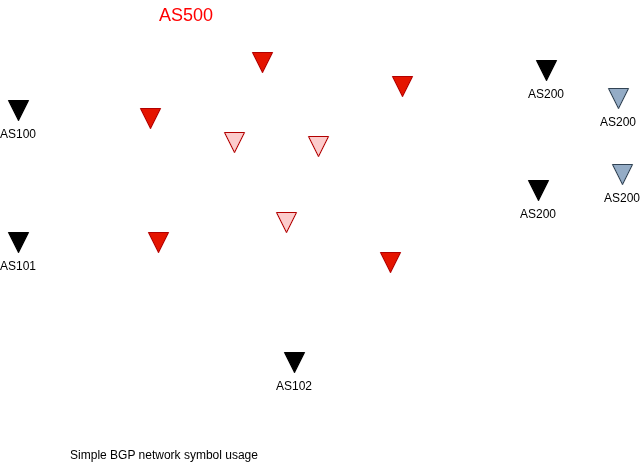
\includegraphics[width=0.7\linewidth]{bgp2.png} % https://drive.google.com/file/d/1EccfKdXZZyW0LT6cPnmi5AjUfwFKyOSz
    \caption{BGP example network}
    \label{fig:diag1}
\end{figure}

In this minimal diagram, there are only the core elements - BGP speakers. Border routers (ASBRs) are shown in strong colours, while internal IBGP-only peers are shown as pale.  Where needed, an AS number is attached to a BGP speaker, but generally colour is sufficient to distinguish AS membership.  The `missing elements' in this diagram are the peering links; a few links are added in the next diagram:\ref{fig:diag2}.  But notice that even in this quite `simple' network, showing all of the internal BGP links would be tedious and unhelpful.  So, in general, the existence of IBGP links is left implied, except in cases where it aids the argument.

\begin{figure}[H]
    \centering
    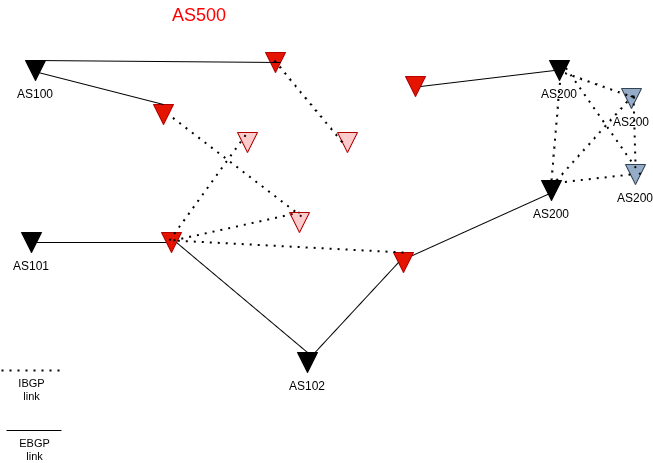
\includegraphics[width=0.7\linewidth]{bgp3.png}
    \caption{BGP example network - with some peer links}
    \label{fig:diag2}
\end{figure}

Here is a simpler, complete, network, showing the usually suppressed IBGP links:
\begin{figure}[H]
    \centering
    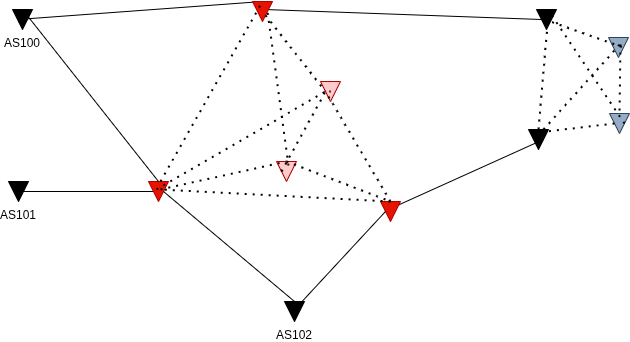
\includegraphics[width=0.7\linewidth]{bgp4.png} % https://drive.google.com/file/d/16C6qxZ84SvLd6x6U58ob4-CbPgehXUmq
    \caption{simpler BGP network, showing all peer links}
    \label{fig:diag3}
\end{figure}


\bigskip

For completeness, the more complex network of Figure \ref{fig:diag3} is presented again below, in Figure \ref{fig:diag4}, restructured using route reflection to reduce the number of BGP peering links.  Note that the difference between these networks,  Figure \ref{fig:diag3} and  Figure \ref{fig:diag4}, is only visible externally, and significant from a BGP configuration and state level - as routing systems they behave identically. `

\begin{figure}[H]
    \centering
    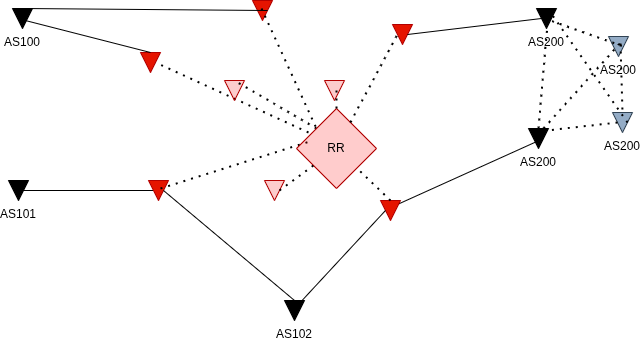
\includegraphics[width=0.7\linewidth]{bgp5.png}
    \caption{fully graphed BGP network, with Route Reflector}
    \label{fig:diag4}
\end{figure}

In all of these diagrams the network links shown represent only signalling connections, although in the case of \ref{fig:diag3} there is a one-to-one relation between  user-plane links and control-plane links, and likely even one-to-one relation to physical links.\footnote{In general, in larger AS systems, the IBGP associations are not direct, because the end-to-end paths between ASBRs are indirect.  Otherwise, there would be no need for either core routers, or even any IGP, e.g., OSPF, IS-IS, \ldots. \\
In contrast, EBGP links are almost invariably direct, both at signalling and forwarding plane level (IXP Route Servers excepted).}

But in fact the core AS in \ref{fig:diag4} will surely have L2 forwarding connections between every node, and also internal routing associations (OSPF or IS-IS) between all such connected nodes.

Note that there is no ambiguity whatsoever to these diagrams, even when no IBGP links are shown, in any cases, with or without Route Reflectors.


    \clearpage
    \singlespacing
	\tableofcontents %\clearpage
    %\addtotoc{List of tables}{\listoftables}
    %\addtotoc{List of figures}{\listoffigures}
    \mainmatter
    \doublespacing
    \chapter{Introduction}
\thispagestyle{empty} %not enumerate the first page
% \textcolor{red}{DH: some changes have been made from here, but are not marked in red.}

Modern life depends on the public Internet in myriad ways, seen and unseen.
The Internet is as important to modern life as other utilities such as power, water or transport, but it is more complex, diverse, pervasive and globally interconnected than any other utility, and arguably more vulnerable to unintentional or malicious disruption.
Whilst conventional utilities such as power, water, etc. are often provided by \emph{interconnected} large and complex organisations and systems, they can, and sometimes do, operate well enough when higher level interconnections fail, and isolated partitions are formed.
The Internet is very different - its \emph{essence} is in its complete interconnection, at national, continental or global scope.
Without constant and reliable interconnection between all component networks, much, and ultimately all, value is lost.
This sets it apart from most other utilities.
\medskip

Whilst the links that interconnect the networks forming the Internet are massive in terms of bandwidth - 100s of Gbps, growing towards Tbps - they would remain empty without \emph{inter-network control traffic}.
The direction and control of these massive network traffic flows between the networks, which collectively comprise the Internet, is called \emph{Inter Domain Routing} (IDR), and the specific mechanisms that direct end-user network traffic over viable end-to-end paths are called \emph{exterior gateway protocols} (EGPs).
In the Internet there is in fact only one EGP protocol: that protocol is the Border Gateway Protocol, or simply ‘BGP’, and it has remained largely unchanged since it was first deployed nearly a quarter of a century ago.
\medskip

The topic of this thesis is the quest to maintain and improve the performance and reliability of Internet Inter Domain Routing, and thereby also the quality of the services that rely on the Internet, through the application of ‘programmability’ to the operation of Inter Domain Routing.
\medskip

\textbf{Motivation - 1}
Organisations and individuals across the globe rely on the Internet for an ever increasing range of services, and it is increasingly the case that the dependence is total - in many cases, Internet service failure can completely disrupt the operation or delivery of an entire range of services or products, with no practical fall back.
In the earlier stages of Internet adoption it was largely commercial concerns that adopted Internet processes, which still left open alternate `legacy' channels for customers unable or unwilling to use the Internet, albeit with possibly less choice and on less favourable terms, but in more recent times the Internet has become essential for many non-commercial aspects of everyday life, including socialising and use of public services.
For most of the history of Internet evolution, large volumes of interaction remained channelled though non-Internet channels; so the dependencies were contained, because alternate servicing channels remained in use, with sufficient capacity to support at least a basic level of service.
However, the shift to Internet as a default channel for so many aspects of commerce and service access has now reached the stage at which society cannot function unaffected for long without the Internet - and were it to be permanently disabled, many organisations would surely go out of business, whilst many more would need to recruit additional staff, and (re-)open sites for providing service directly, or by telephone or postal services - with obvious ultimate impact on consumers.
One of the most obvious, devastating and immediate impacts would be to commerce and payments - there might simply be insufficient `real' money to support even offline commerce.
%\medskip
So, the potential economic and social impact from Internet failures is thus far higher than it was at the time that the structure and technology of the current Internet emerged.
Yet the security design and vulnerabilities of the global Internet interconnection system are unchanged since its inception 25 years ago.
\footnote{https://blog.apnic.net/2019/09/19/why-is-securing-bgp-just-so-damn-hard}
\medskip

\textbf{Historical Context}

It would be wrong to suggest that there has been \emph{no} positive movement towards a more reliable internet in that time, but the changes that have been made are small and incremental, and many of the fundamental vulnerabilities that existed 20 years ago are still present today, whilst the maliciously motivated challenges have certainly increased.
In consequence, Internet services are not substantially more secure or reliable than they were so long ago.
It is at least plausible to suggest that the reason for this inertia, lies, perversely, in the strength of the original architecture: in contrast, video distribution technology has seen many changes, from the VHS vs. BetaMAX tape format wars of the late 1970s, through DVD and Blu-Ray to Netflix, and at every stage the entire previous ecosystem - hardware, software, etc - was replaced from scratch; the incompatibility between generations was total.
A similar narrative applies to mobile telephony: since analogue phone service were introduced around 1983, consumers and service providers have gone through at least 5 complete upgrade cycles.
In contrast, end-user equipment compatibility on the Internet is effectively total across time as well as space - not only can any Internet endpoint of today contact any other, across the entire globe, the same holds true across all time, ever since TCP and IP were defined in 1981.
Even the service providers' network-to-network compatibility has changed once, in a backwards compatible way, since the first EGP (called `EGP'), was defined in 1982.
Furthermore, there is no serious current proposal to replace TCP/IP with something `better', and TCP/IP is as prevalent in private networks as it is in public ones.\footnote{QUIC emerged during the writing of this thesis \ldots}
Only Ethernet has as long and pervasive a history of dominance - the case might even be made that the architecture should actually be named TCP/IP/Ethernet, given how closely they are integrated and how complementary their roles.
Certainly, the architectural principle which distinguishes yet unites TCP/IP and Ethernet is an essential element of the overall `TCP/IP architecture'.
\medskip

\textbf{Motivation - 2}
The foregoing discussion of the vulnerability of society and the global economy to Internet failures is motivation enough for academic work in myriad areas of research, of which communications and networking is but one, and within just the field of network research there can be many angles of approach to this important topic, with varying degrees of immediate applicability.
But what is surely evident when simultaneously considering both this high level of vulnerability and risk, and the historical and commercial context just outlined, is a pressing need for \emph{incremental}, and thus \emph{deployable}, approaches to improving Internet resilience.
The later related work survey is remarkable in that it finds no recent prior work that directly approaches this issue in these terms - there are many contributions in the wider literature on more secure future architectures, on analyses of vulnerabilities and attacks, and on schemes for rapid and accurate detection of routing failures; and there is also applied/practical work on other, non-Internet transit, network resilience and routing enhancement (e.g. for data-centre, IXP and Internet edge), but nothing which is both practical and directly relevant.
Is this problem intractable, or just uninteresting? Or is it perhaps the case that the topic has been categorised as `engineering' rather than `research'.
(This dichotomy is discussed in more depth in a later chapter.)
\medskip

The related work may be summarised thus: in 2006 Karlin, Forrest \& Rexford published ``Pretty good BGP: Improving BGP by cautiously adopting routes" \cite{Karlin2006} - 12 years later, in 2018, Sermpezis, Kotronis, Gigis et al. published ``ARTEMIS: Neutralising BGP hijacking within a minute" \cite{Sermpezis2018}.
Both research groups followed similar paths, to arrive at the same, perhaps unsurprising, conclusion that there exist simple and effective techniques that use readily accessible data to yield quantitatively better BGP routing outcomes than can be achieved by any unaugmented network of legacy BGP routers. A literature search reveals many more papers published between these two, which converge towards the same consistent conclusion.
Collectively, they represent a rich and diverse set of strategies for improving internet routing. What is striking, however, is that even more than a decade after the first paper was published there has been no material progress towards applying these insights in the real world; nor even, it would seem, has there been any curiosity about how that might be achieved.
Indeed, the 2006 paper has a more concrete and detailed approach to the subject than almost any paper published since.
(See the related work chapter for more on this topic).
The last point to be drawn here is this compelling insight from Karlin, Forrest \& Rexford (2006) - in their words, `(the) Importance of a Collective Response':
\emph{"PGBGP can protect 97\% of ASs from malicious prefix routes and 85\% from bogus sub-prefix routes when deployed only on the 62 core ASs in our study network. If PGBGP were deployed on all ASs, both numbers would exceed 99\%"}.
This paper clearly explains why there is so little merit in optimising just a subset of transit networks - because unless the response is \emph{collective} there can be no effective response - hence the \emph{only} useful strategy is one which can be adopted by all transit service providers, not just a few.
\medskip
This is the central challenge for this thesis: to discover, if possible, a strategy which might realistically be adopted by all transit networks.
\footnote {ROA/RPKI was defined in 2012 - whilst it is in moderate use to day (see \url{https://rpki-monitor.antd.nist.gov/}) - less than 20\% of the Internet address space is even registered for protection, whilst the actual level use by network operators of the registry is harder to measure but seems unlikely to be much higher if at all than the level of use by address space owners.
	ROA has the strong advantage that it can be deployed without disruption and incrementally, and does not directly affect BGP operation in any way.
	Secure-BGP is more recent (RFC8205 in 2017, under active investigation since 2000, IETF SIDR WG since 2006), and much more intrusive.
	There are no reports that BGPsec is deployed anywhere in the Internet today, which is not surprising since no commercial router vendor supports the protocol. (see \url{https://pc.nanog.org/static/published/meetings/NANOG2019/1840/20180921\_Kosters\_Security\_Q\_A\_And\_v1.pdf})  \url{https://blog.apnic.net/2019/09/19/why-is-securing-bgp-just-so-damn-hard/ is also authoritative and relevant}}
\medskip

%\textcolor{red}{DH: edited up to here now ...}

\textbf{Programmability} The term ‘programmability’ requires clarification and justification in order to differentiate ‘Programmable Internet Routing’ (PIR) from the prevalent routing control model referred to here as ‘Static Internet Routing’.
Another important question is motivation: why is Programmable IDR 
%%% \textcolor{red}{[expand / explain (again) IDR]}
needed.
This is a broader topic and more familiar - briefly, security, reliability and Quality of Service are explicit target attributes, although arguably the objective parameter is cost of delivery, and the others are constraints, which need to be met rather than maximised.
\medskip

\textbf{Scope} In this thesis there is a strong need for definition and scope of both the problem space and solution space: the Internet is not the only network, nor even the only globally connected network, and there are arguments in support of the proposition that the current Internet cannot meet the future demands, or even all the current demands, for ‘Internet like’ services - perhaps necessitating development and deployment of an entirely new, ‘clean slate’, ‘Future Internet architecture’.
It is not the intent here (yet!) to take sides in that debate; nonetheless an important contribution to that debate is the establishment of the limits inherent in the existing technology, and such a contribution may even help shape the direction of Future Internet work.

In fact, this thesis makes the argument that the problem space (or solution space) definition question is a central issue in making sense of the complex and sometimes confusing topic of Future Internet (or \emph{new network}) evolution: but, perhaps unfortunately (at least for academics and engineers), it is economic, social and political considerations that will dictate in the broadest sense what network services will be deployed as Internet services, and how precisely they are delivered.
\medskip

\textbf{The prospectus}
The thesis makes the argument that a new \emph{evolved} architecture is possible and beneficial - an architecture which is an \emph{incremental} evolution of existing transit and ISP designs,
which need not impact on the stability and performance of existing designs, yet can improve resilience to routing failures and attacks, and also represents an intermediate step to a full ‘SDN’ network architecture.
\medskip

\textbf{The architecture}
The scope of the new architecture is the individual transit ISP.
The architecture has two aspects - monitoring and control.
Monitoring is conceptually simple - every ASBR has a monitoring link to a control point, and that monitoring link uses one of two standardised protocols - BMP or BGP/ADD-PATH.
Control links simply follow the reverse paths to the monitoring links - the control links are technically even simpler than monitoring links, using only standard BGP.
However, the detailed specification of how BGP control sessions can effect the required results, reliably, consistently and without undesirable adverse impact is more complex.
The proposed architecture is \emph{delocalised} rather than centralized.
This means that it can scale and implement resilience, while implementing a \emph{logically centralized} control model.
\medskip

\textbf{The research programme} The research addresses - \emph{Scoping, design, implementation, observation, experimentation and evaluation}

The work reported in this thesis covers:
\begin{itemize}[noitemsep,nolistsep]
	\item{analysis of internet routing traffic (‘routeviews’ MRT data)
	      }\item{MRT analysis tools, which use shared libraries from other parts of the project
	      }\item{an implementation of a full BGP speaker which implements Programmable Internet Routing - PIR: this BGP speaker is written entirely in the functional language Haskell
	      }\item{an experimental infrastructure which allows arbitrary topologies to be assembled with BGP speakers including both PIR and also widely used ‘production quality’ BGP speakers (bird, frr, openBGPd, and virtualised instances of Cisco and Juniper core routers)
	      }\item{a BGP performance and scale test system
	      }\item{a reference minimal BGP speaker which is used as a baseline system to validate the performance test tool
	      }\item{an evaluation of the performance of the PIR system alongside the other BGP speakers
	      }\item{an evaluation of the performance requirements and limits of BGP speakers in real world contexts e.g. IXP and core transit networks
	      }\item{proposal, analysis and evaluation of the architectures and performance constraints of hyperscale BGP speakers
	      }\item{an evaluation of the operation and performance of the PIR architecture proposed and implemented in this thesis}

\end{itemize}

\textbf{Motivation}
The motivation is to investigate and, for the first time, to build and demonstrate an evolved architecture, and an assessment framework that checks the `real-worldliness' of the technical system that has been developed. The work covers: requirements, design and implementation of a PIR architecture;
QoS - Internet application QoS requirements - implications for BGP interconnection;
implementation and Optimisation of BGP speakers - analysis informed by Internet measurement studies and real world code implementations of performance bottlenecks in functional and procedural implementations, including an overview of advantages and disadvantages of a FP Haskell implementation.

% \textcolor{red}{DH: I have added text to the paragraph above -- please check whether you like what I've done here (or not ...).}
% \NH{yes, thanks...}

\section{Background}
\textbf{SDN and Future Internet}
Both SDN and Future Internet (FI) represent complementary strands of research that are intended as pathfinders for the direction of network evolution - SDN is arguably a ‘bottom-up' approach, and FI a ‘top down’ approach.
(both, and their relation to this work, are examined in more detail later). Meanwhile, this thesis addresses the same issues as in FI and much of SDN, and proposes an architecture that is both a form of SDN, but also enables an evolution from conventional ‘legacy’ networks to a more conventionally conceived ‘SDN’ network.
The relevance to FI is perhaps philosophical (as is FI research in some instances) - FI aims to articulate and then address current limitations of the Internet, and future requirements, with an implied assumption that resolution of these issues requires ‘architectural’ change.
The prospectus in this thesis is at odds with FI - it aims to make the existing architecture as good as it can be, and argues that ‘Future Network’ and ‘Future Internet’ are not synonymous, but can coexist.
In doing so it may effectively undermine much FI work from an existential perspective.
However, both SDN and FI are important influences on this work - the intention is to deliver on the promise of SDN and to resolve the challenges of FI by distinguishing more clearly the services and capabilities which are (and are not) ‘Internet’ in nature, and to show the natural limitations that define the boundary between them.
\medskip

%\textcolor{red}{DH: edited up to here now ...}

\textbf{Commercial aspects}
Even once the Internet achieved ubiquitous global reach, it continued to evolve by expanding the services it could support, gradually and unevenly across the Internet, displacing other networks as it became fast enough, cheap enough and reliable enough to support the new services.
An essential aspect of this evolution has been the development of economic models and network designs that enable both network providers and service providers to remain profitable without relying on end-user charging other than essentially flat rate tariffs.
An orthogonal operational and commercial premise is the charging model for traffic between networks - the charging system referred to as 95th percentile billing - which assigns charging based on peak flows, reflecting the fact that network capacity has to be provided based on expected peaks rather than averaged flow rates.
The result of the 95th percentile transit charging model, and its combination with un-metered end-user service, is a very different model than one which would assign charges based on resource reservation. This represents a very high hurdle to acceptance for any future network architecture; it would dictate resource reservation as a means towards improved QoS for specific services.
This ‘flat-rate’ charging model fits the ‘best-effort’ service proposition - and it is hard to foresee a change from ‘best-effort’ without a corresponding change in charging and cost allocation principles.
\medskip

\textbf{Organisational Inertia}
Resistance to change - the basic principles of network operation have changed very little in decades.
The reasons for this inertia are complex and include:
\begin{itemize}[noitemsep,nolistsep]
	\item{long experience and large investment in existing technologies and architectures}
	\item{incumbent equipment vendors reluctance to facilitate or endorse technical developments that could threaten their commercial interests}
	\item{low appetite for risk or innovation within the network operator community}
	\item{an absence of commercial or even experimental alternative architectures and solutions}
	\item{resistance to solutions which rely on centralized management systems, which are seen as inherently less resilient than existing distributed architectures}
	\item{focus on other areas of technical development, e.g. MPLS and TE.}
	\medskip
\end{itemize}

\textbf{A fork in the road (evolution vs. revolution)} The foregoing arguments lead one to the conclusion that programs for Internet service improvement fall into just two, quite diverse, categories. These can loosely be classified as evolution or revolution - the essential point being that the combination of technologies and supporting commercial and organisational structures that compose the current Internet are very much entangled around the existing design. Thus, a significant change that is both end-to-end backwards compatible and also revolutionary in terms of upgraded service characteristics, seems very unlikely.
The hybrid (and in this view a more plausible) ‘Internet evolution’ road-map is arguably already in progress. This is one in which individual network service providers deliver ‘vanilla Internet’ service as an overlay service over an enhanced access network, alongside differentiated services which are more restricted in their reach - either only within the local domain, or only over interconnection with selected partners.
Enhanced services might be presented as regular IP, addressable using public IP addresses but in reality routed and terminated differently to other Internet traffic.

%\textcolor{red}{DH: edited up to here now ...}

New applications, for example those that might need to signal QoS requirements, might also be delivered through the legacy IP address space without major change to host system network stacks, while yet other services might follow the route of entirely new protocols and interfaces to the end system, running in parallel to legacy Internet service delivery.
Of course, there is nothing new in this hybrid service proposition: early consumer ADSL services did exactly this, reserving a high speed channel for delivery of locally hosted services such as VoD and telephony, and today's content providers, such as Netflix, also adopt this model, under the publicly addressed/locally terminated architecture, embedded in access network providers' infrastructure.
This may be bad news for the Future Internet architecture proponents, because it undermines their argument for re-engineering the Internet from scratch - but it also offers the possibility that parallel globally connected Internets could come into existence - some perhaps offering intrinsic security, or built-in edge computing, or limited but still multi-domain low-latency services - each with different business models than the current, default, `best-effort' and `all-you-can-eat' approach.
The common theme in all of these ideas is the continued usage wherever possible of public Internet address space, and TCP/IP as a service API.
This makes explicit a dichotomy between IP as an API and IP as an end-to-end architecture.
The end user may consume multiple ‘internet’ services, unaware of the diversity, as long as the service interface remains the same and the charging models are distinct but compatible with the commercial relationships between consumer, access provider, and end service provider.
\medskip

\textbf{Defining the problem space} Transit networks exist out of necessity: there are too many end-system networks ($\sim$ 50,000) to permit 1:1 peer links between them all.
A ‘radical’ counter proposal would be to allow every end AS to build (virtual) L2 links to every other such network - but if there were competing transit L2 providers (think: IXP!) then the problem of choosing which L2 provider reduces to exactly the BGP transit architecture with a maximal AS path length of 2.
But of course that would require ubiquitous L2 providers with complete global connectivity to all end ASes - which is infeasible - not least because small ASes do not want or need to have the commercial complexity of connecting to every ‘tier 0’ transit. Thus a hierarchy is inevitable, which leads to the problem of interconnecting the hierarchy, which eventually leads back to the BGP transit hierarchy that we sought to eliminate.
A challenge to this could be constructed from an analysis of end-ASes by classifying as ‘eyeball (access)’ and service/content provider - this reduces the scale of the interconnection matrix (from (n+i)2) to n x m, at least for the bulk of traffic - but the reduction is still not great enough to make a full mesh remotely practicable, even if this simplistic partition were valid.
But more problematic than the technical and operational complexity would be the commercial complexity - who pays who, how much? - and, finally, consider the additional signalling traffic required to manage all of these connections - which would far outweigh actual user traffic for over 99\% of all connections.
\medskip

\textbf{‘The death of transit’} It is certainly true that the relative \emph{volume} of indirect Internet traffic is reducing, driven by the rise of IXPs and CDNs, the concentration of consumer Internet activity into small number of very large content and service providers, and the increasing use of cloud based systems to host content on behalf of smaller organisations.
%%% \textcolor{red}{[Have you been consistent with the use of the `z' form?]}
%%% \NH{yes, it is fixed throughout now}

So it is wise to ask whether this means that the aggregate impact of the vulnerability to internet failures described above is actually lower than it would appear, and that perhaps the most important or widely used services are already increasingly less susceptible to the impact of interruptions rooted in the IDR system.
The answer is obvious from a qualitative perspective: embedded content and direct or IXP inter-mediated peering is already responsible for a high volume of both traffic and transactions - and possibly an important recent trend is the growth in the membership of IXPs from larger companies. Thus it is undoubtedly the case that for many consumers and businesses, under `normal' circumstances, much Internet traffic already bypasses transit networks entirely. 

%%% \textcolor{red}{[Do you think most readers will understand `transit'?]}
%%% \NH{Updated, please review...}
The question is only how long (and tall) is the fat tail of traffic which still must transit transit.
The subject of exactly which services, and for whom, will remain indefinitely vulnerable to transit traffic issues is a worthy subject for further study - as evidenced by the fact that it was hard to find a good answer to this question here.
The data from a 2019 presentation at NANOG from Nokia is perhaps a good authority as any: \url{https://pc.nanog.org/static/published/meetings/NANOG76/1972/20190610\_Labovitz\_Internet\_Traffic\_2009-2019\_v1.pdf} - this report shows continuing growth in transit traffic, albeit at lower rates than total end-user traffic levels.
(Even finding authoritative data on transit traffic volumes is difficult.)
%\medskip
So, it may be that the \emph{‘The death of transit’} is also \emph{‘The death of Future Internet’}, as single-AS-hop or zero-AS-hop paths become the norm for all significant Internet services.
Interestingly this is almost exactly the implied universal mitigation in the Artemis
%%% \textcolor{red}{[Explain what this is ...]}
%%% \NH{I made it more explict that this is a paper I review in depth...}
paper - where, for hijacked prefix owners the preferred, and, in most cases,
the only solution is seen to be \emph{`Outsourcing mitigation with MOAS announcements'}.  (The Artemis paper is reviewed in the later chapter `Related Work').
In other words, the owner of specific prefixes delegates authority \emph{to another AS} to originate their prefixes, at as many locations - in practice IXPs - as the mitigation service provider can access.
The consequence of this strategy is an even more rapid evolution towards a `two-tier' Internet, in which only the most marginally valued services are accessed via transit.
The great enabler of this evolution is of course `public cloud' services, which enable virtually any provider of Internet based services to deploy their applications or content without the need to separately implement Internet access.
It maybe that this trend will so reduce the scope for malicious actors to cause widespread damage or yield significant fraudulent gains that the level of routing attacks will diminish so that the techniques advocated in this thesis will prove ultimately unnecessary.
However, current reports show no signs of such a reduction in routing attacks yet, so it still seems worthwhile to pursue the goal that is set.

% \paragraph{Narrowing down the topic - and some historical context} \textcolor{red}{[I need you to make this more readable.]}
% {\color{blue}{I understand the grammar here is odd/needs fixing, is that the point?}}
% - i.e. academics looked at programmability several times, but always came up with solutions which are effectively big-bang - they keep BGP as a protocol and as a device level specification, but substitute the distributed routing decision system with completely centralized control.
% It illustrates the flexibility of BGP but is not viable for existing networks, and does not solve the problem of incrementally improving the quality of routing decisions.

% \subparagraph{Conclusion}
% No one has investigated how to work synergistically with an IBGP mesh,
% \textcolor{red}{[Again, you have to make this more readable, and explain what IBGP means ...]}
% \NH{[Re IBGP, it's difficult to know what to do here when I devote several pages later to what IBGP is.  Should I write a brief summary of BGP here in the Introduction, so that the meaning is clear?  I worry that if the reader doesn't know already at a basic level, then the rest of the thesis would be rather hard to take in. Is it that the Introduction would be more widely understandable?]}
% \NHx{[Regarding the substance of the paragraph, I can write more text which might be more accessible, but I hope that the form here would be understandable by a reader with the background.  I think on reflection that I should merge the text under the two headings \textbf{Narrowing down the topic - and some historical context} and \textbf{Conclusion}, but I want to clarify with you about the questions above... ]}
% possibly because without access to external routing state there is little gain - the analysis suggests that for most problems the best possible strategy is simply promoting a second best route - but that gaining reliable access to a second best route was not possible in the context of BGP networks until at least 2016, when ADD-PATH and BMP were standardised and widely implemented.

%%% \NH{original text reworded entirely, now left only in comments}
\paragraph{Conclusion}

In the past, academic researchers explored programmability as a means to enhance Internet architecture, resilience, and performance. However, the resulting proposals often necessitated "big-bang" deployments rather than incremental changes. For example, solutions like Routing Control Platforms (RCPs) \cite{Feamster2004} retained the Border Gateway Protocol (BGP) at the protocol and device level but substituted its distributed routing decision-making system with entirely centralized control. While effectively demonstrating BGP's adaptability as a protocol, this type of approach is not practical for deployment in existing networks and does not address the challenge of incrementally enhancing the quality of routing decisions.

Within an Autonomous System (AS), the specific BGP variant used is Internal BGP (IBGP). Notably, there is a scarcity of reported research investigating how to work synergistically with an existing IBGP mesh, in contrast to work done for other protocols, such as Vissicchio et al.'s 'Fibbing' approach for OSPF \cite{Vissicchio2015c}. This lack of focus on IBGP may be because improving upon the standard route selection process is challenging without complete and reliable access to external routing state information, which is only \textit{consistently} available at the border routers, but not propagated unless a border router has already selected a route as optimal. Detailed analysis suggests that for many common routing problems, the most effective strategy is often to promote the second-best available route, however, reliably accessing such second-best routes within IBGP networks was not feasible until the standardisation and subsequent commercial availability of technologies like ADD-PATH, and the BGP Monitoring Protocol (BMP), starting around 2016.
\medskip

%\textcolor{red}{DH: edited up to here now ...}

\section{Thesis organisation}
\textbf{Chapter 2 - Background}
Chapter 2 describes the context of the thesis and expands on some topics already mention elsewhere in the Introduction.
This includes multiple themes, as follows:
\begin{itemize}[noitemsep,nolistsep]
	\item{structure and organisation of the current Internet;
	      }\item{brief historical summary focusing on how the evolution of the Internet and its underlying technologies have been shaped by changing requirements.
	            This includes a mention of ‘flattening’ and the ‘death of transit’ perspective;
	      }\item{discussion of BGP - its role, and how protocol specification influences and is influenced by the application (IDR);
	      }\item{a short description of how IDR and BGP are used - what issues arise, and how BGP and the policies it enables address issues (‘how does BGP enable ‘policy’?’);
	      }\item{description of the key challenges in IDR today (QoS / security / availability / resilience / economic viability / surveillance, control, governance and ownership);
	            What are the service goals for the Internet?  Does this question even make sense?  How is the delivery of those goals enabled, or not, by the current architecture?
	      }\item{a short introduction to SDN - what is it and why is it relevant to this thesis?
	      }\item{IETF - a review of the role of the IETF and the current and historical contributions to the topic form the IETF.}

	%(the NIST document gives some good pointers!) <Note this could be considered ‘related work’.>
	\medskip
\end{itemize}

\textbf{Chapter 3 - Related work}
Some themes from chapter 2 re-emerge here - but the leading question is what problems are the earlier researchers intending to address, and what role if any does SDN play?

%%% \textcolor{red}{[This surely needs to be expanded somewhat ...]}
%%% \NH{[How many words?  Worried about duplication, worried about obscuring the point which is about organisation...]}
\medskip

\textbf{Chapter 4 - Research Context}
The academic backdrop to this thesis lies in the research fields of `SDN' and `Future Internet', which represent respectively a `bottom-up' and `top-down' prospectus for network evolution.
This chapter explores some contrasting perspectives on the fundamental issues in evolving networks and network technology for supporting the changing ways in which society uses digital technology. It also addresses the `virtuous circle' whereby technology change drives the creation of `new services' and new ways of interacting, while the changing social exploitation of the technology drives yet further technological development. An important question is ``how well does the academic prospectus align with the realities of social and technological change?".
This leads naturally to the practical themes of the thesis: what problems are presented by current technology, specifically in the field of Internet service delivery; how can these challenges be addressed by the application of pragmatic technological innovation, crafted to address the organisational and economic constraints that so challenge other academic proposals?
%- perhaps fatally, if the arguments presented in this chapter and in the preceding chapter on related work.

\textbf{Chapter 5 - On BGP}
There exist many books and publications on BGP, with a variety of aims and focus:
\begin{myitemize}
	\item BGP as a protocol - stability, performance, and simply `how it works';
	\item BGP applications - core Internet routing (IDR), data-centre applications, customer (MPLS-/L3)VPN, EVPN and layer 2 VPNs and scaling;
	\item Internet structure - peering, `flattening', security, economics, topology evolution, resilience;
	\item implementation.
\end{myitemize}

For many purposes it is possible to treat BGP routers simply as agents that exchange abstracted route objects - objects with the well known properties of AS paths, local preference, BGP communities etc., while passing over any detailed consideration of the dynamics of coordinating simultaneous high volumes of input and output messages, with multiple peers, and the necessary rules that ensure consistent and convergent behaviour.

It is also possible to study BGP systems in great depth, without understanding or considering the peculiar and different behaviour of BGP as an AS \textit{internal} protocol, its interaction with IGPs - other internal routing protocols, operating concurrently in the same AS, and the mechanisms employed within an AS to implement the essential distinctive behaviours towards `customers', `peers' and `providers'.
Another complementary domain is the internal administration of BGP routers within an AS in order to achieve desired outcomes for traffic flows \textit{with other ASes}.
All of these domains fall loosely into the category of what is sometime called `BGP policy' - but none of them relate to the challenges faced by an implementer of BGP.
Fortunately, the implementer need understand nothing of these issues and problems in order to build not only a passable BGP, but actually a BGP that is as good as, or `better' than, any existing BGP.
However, the bridge between the `eyes-down' world of the BGP implementer and the `eyes-up, looking outward' perspective of the network architect or manager is the murky `BGP policy engine' - the part of a BGP system in which every implementation differs, requiring the implementer to define some form of `programming language', or DSL. This vitally important topic is one subject of the practical work of this thesis, and is also one of just two areas that distinguish BGP implementations from each other, offering scope for innovation, differentiation and, if done wrongly, can lead to catastrophic network failures.

In this thesis, the presentation of BGP is oriented primarily towards the eyes-down implementation aspects, relevant to the work presented, and secondarily as an overview of operational principle that serves as a background to the applications developed; it also outlines ways in which the conventional `policy engine' limits the scope of control and flexibility.

\medskip

Note: The description here of core BGP is no substitute for reading the original, succinct and lucid RFC, RFC4271 \cite{rfc4271},it rather attempts to explain some of the unstated reasoning and implications of that RFC.

\medskip

The last aspect presented is an exposition of the `beautiful' way in which BGP distributes decision-making over an entire AS, enabling huge scalability and resilience, but also making any proposition of creating a single, central, point of control seemingly impossible, without losing the benefits of this distributed architecture.

\medskip

% \textbf{Chapter 6 - Design}
% `Design’ may not be adequate to describe the scope of this chapter.
% The chapter starts with a restatement and elaboration of the ‘problem statement’ already defined in the Introduction
% %%% \textcolor{red}{[Check that it is here, and also make sure you introduce IDR (again?).]}
% , which is not just the external challenges - i.e. ‘better’ IDR - but why it is difficult to make IDR better.
% Part of this chapter develops the argument that the internal BGP based architecture of transit networks is not just one of a large spectrum of design solutions but an inevitable fixed-point/singular outcome of some fundamental principles - for example the distributed decision process makes it hard to reason about received routes with full context.
% The related work gives examples that underline the difficulty of changing the architecture in a non-disruptive, evolutionary, way.
% Later parts of the design move onto the architecture of the proposed solution - the externally observable behaviour (route poisoning) - the internal implementation - what is PIR?, and what are the requirements and constraints for PIR - and what are the design choices available?
% The proposed design and mechanism are also described - with limitations and performance constraints, and also consistency, integrity, latency, and fail-safe operation.
% \medskip

% \textbf{Chapter 6 - Implementation}
% There are multiple implementation aspects.
% The first is \hbgp.
% The implementation in Haskell is motivated and described, explaining the benefits and potential pitfalls, and also the overall functional decomposition of the problem.
% 	[An appendix describes some details of the work.]

% The second aspect of implementation is the test framework.
% This implementation starts with a discussion of the test requirements for the framework - what are the aspects of \hbgp that should be evaluated?
% How can these metrics be observed? What are the challenges in making accurate and verifiable measurements?
% How does the design address these requirements?

% The third implementation aspect is the reference implementation.
% The test framework allows \hbgp to be benchmarked against commercial and open source production quality BGP speakers.
% The results are illuminating but give rise to the need to calibrate the test framework in order to gain assurance that the observed performance metrics are not artefacts of the measurement system.
% The reference implementation developed for this purpose is a simple `C’ language BGP speaker.
% As well as allowing the calibration and verification of the test framework, the implementation of a stripped down BGP speaker optimized for performance sheds light on the limitations of both \hbgp and the tested production BGP speakers.
% \medskip

% \textbf{Chapter 6 - Evaluation}
% There are two themes in the category of evaluation - the first is the evaluation of \hbgp to demonstrate its capabilities to fulfil the role required for PIR.
% This evaluation is a combination of functional and performance testing - it shows that \hbgp can be used to augment a conventional transit network to create an instance of PIR that exhibits complex and more effective routing behaviour than is possible in the conventional network alone.
% The second aspect of the evaluation is the benchmarking of \hbgp with other production grade BGP speakers and the reference BGP speaker.
% This evaluation shows that the goal of implementing BGP policy using high level language constructs is viable, and also sheds useful light on the fundamental limitations of single threaded BGP speakers and the potential for building higher performance BGP speakers using optimized distributed or concurrent processing techniques.
% \medskip

% \textbf{Chapter 7 - Conclusion}
% The Internet and its uses continue to expand and evolve, whilst its technical foundations remain in many ways unchanged.
% In the eyes of many commentators, the capacity of the Internet to accommodate change and improvement is restricted by fundamental aspects of those foundations, and BGP and its associated architecture is often seen as one of the major obstacles to evolution.
% This thesis aims to contradict such a view and to show that BGP enabled systems are capable of evolving smoothly into a more agile and flexible ecosystem without the need for radical change in protocols, architectures or infrastructure and investment.
% This final chapter discusses the role for SDN in a `Future Internet’ and proposes a more evolutionary than revolutionary approach, which still enables radical change to the Internet and Internet-based services.
% In the more immediate future there is a need for improved routing policy -- and a large amount of work already exists, showing how to derive and define better policy. However, there is an absence of mechanisms in existing networks and equipment to apply these ideas.
% %%% \textcolor{red}{[Quote Artemis, pretty good BGP and the NIST document references.]}
% %%% \NH{Artemis is the only paper I mention elsewhere which corresponds to \textbf{showing how to derive and define better policy}.  I have others in my collection which I could quote if you think worth digging them out.  If I do I should probably also add them into the main Artemis discussion.  Is this what your question means?}
% To address these concerns, a SDN-style approach is attractive, and for new entrants to the field a simple architecture can be proposed, based on a distributed route controller such as first proposed in RCP, in which BGP is used as a south-bound SDN API protocol. 
% %%% \textcolor{red}{[Expand on RCP here.]}
% %%% \NH{again happy to add text but worried about duplication....?}
% Unfortunately, existing large networks are unlikely to adopt this clean-slate approach, and there is a clear need to develop a strategy for evolution from conventional networks towards such an architecture.
% This thesis addresses this difficult and important gap, and in doing so provides two important contributions: the first is a mechanism to upgrade existing transit networks to enable Programmable Routing control, and thus improve the reliability of routing in the Internet today; and the second is the identification of a direct evolutionary path towards a SDN-enabled Future Internet architecture.

% %\textcolor{red}{DH: edited up to here now ...}

\bigskip

\textbf{Chapter 6 - Research Scope}
% `Design’ may not be adequate to describe the scope of this chapter.
This chapter starts with a restatement and elaboration of the ‘problem statement’ already defined in the Introduction,

%%% \textcolor{red}{[Check that it is here, and also make sure you introduce IDR (again?).]}
 which is to say, not just the external challenges - i.e. build a ‘better’ IDR - but why it is so difficult to make IDR better.

 Part of this chapter develops the argument that the internal BGP based architecture of transit networks is not just one of a wide spectrum of design solutions, but an inevitable fixed-point/singular outcome of some fundamental principles - for example, the distributed decision process makes it hard to reason about received routes with full context.

 The earlier chapter on related work gives examples that underline the difficulty of changing the architecture in a non-disruptive, evolutionary, way.

Later parts of the design move onto the architecture of the proposed solution - the externally observable behaviour (route poisoning) - the internal implementation - what is PIR?, and what are the requirements and constraints for PIR - and what are the design choices available?
The proposed design and mechanism are also described - with limitations and performance constraints, and also consistency, integrity, latency, and fail-safe operation.
\medskip

\textbf{Chapter 7 - Implementation}
There are multiple implementation aspects in this Thesis.

The first is \hbgp.
The implementation in Haskell is motivated and described, explaining the benefits and potential pitfalls, and also the overall functional decomposition of the problem.
	% [An appendix describes some details of the work.]

The second aspect of implementation is the test framework.
This implementation starts with a discussion of the test requirements for the framework - what are the aspects of \hbgp that should be evaluated?
How can these metrics be observed? What are the challenges in making accurate and verifiable measurements?
How does the design address these requirements?

The third implementation aspect is a performance benchmark reference BGP implementation.
The performance test framework allows \hbgp to be benchmarked against commercial and open source production quality BGP speakers.
The results are illuminating but give rise to the need to calibrate the test framework in order to gain assurance that the observed performance metrics are not artefacts of the measurement system.
The reference implementation developed for this purpose - `kakapo' - is a simple `C’ language BGP speaker.
As well as allowing the calibration and verification of the test framework, the implementation of a stripped down BGP speaker optimised for performance sheds light on the limitations of both \hbgp and the tested production BGP speakers.
\medskip

\textbf{Chapter 8 - Evaluation}
There are two themes in the category of evaluation - the first is the evaluation of \hbgp to demonstrate its capabilities to fulfil the role required for PIR.
This evaluation is a combination of functional and performance testing - it shows that \hbgp can be used to augment a conventional transit network to create an instance of PIR that exhibits complex and more effective routing behaviour than is possible in the conventional network alone.
The second aspect of the evaluation is the benchmarking of \hbgp with other production grade BGP speakers, and with the benchmark reference BGP speaker.
This evaluation shows that the goal of implementing BGP policy using high level language constructs is viable, and also sheds useful light on the fundamental limitations of single threaded BGP speakers and the potential for building higher performance BGP speakers using optimised distributed or concurrent processing techniques.
\medskip

\textbf{Chapter 9 - Conclusion}
The Internet and its uses continue to expand and evolve, whilst its technical foundations remain in many ways unchanged.
In the eyes of many commentators, the capacity of the Internet to accommodate change and improvement is restricted by fundamental aspects of those foundations, and BGP and its associated architecture is often seen as one of the major obstacles to evolution.
This thesis aims to contradict such a view, and to show that BGP enabled systems are capable of evolving smoothly into a more agile and flexible ecosystem, without the need for radical change in protocols, architectures or infrastructure and investment.
This final chapter discusses the role for SDN in a `Future Internet’ and proposes a more evolutionary than revolutionary approach, which still enables radical change to the Internet and Internet-based services.
In the more immediate future there is a need for improved routing policy -- and a large amount of work already exists, showing how to derive and define better policy. However, there is an absence of mechanisms in existing networks and equipment to apply these ideas.
%%% \textcolor{red}{[Quote Artemis, pretty good BGP and the NIST document references.]}
%%% \NH{Artemis is the only paper I mention elsewhere which corresponds to \textbf{showing how to derive and define better policy}.  I have others in my collection which I could quote if you think worth digging them out.  If I do I should probably also add them into the main Artemis discussion.  Is this what your question means?}
To address these concerns, a SDN-style approach is attractive, and for new entrants to the field a simple architecture can be proposed, based on a distributed route controller such as first proposed in RCP, in which BGP is used as a south-bound SDN API protocol.

%%% \textcolor{red}{[Expand on RCP here.]}
%%% \NH{again happy to add text but worried about duplication....?}

Unfortunately, existing large networks are unlikely to adopt this clean-slate approach, and there is a clear need to develop a strategy for evolution from conventional networks towards such an architecture.

This thesis addresses this difficult and important gap, and in doing so provides two important contributions: the first is a mechanism to upgrade existing transit networks to enable Programmable Routing control, and thus improve the reliability of routing in the Internet today; and the second is the identification of a direct evolutionary path towards a SDN-enabled Future Internet architecture.

Finally, an analysis with a wider scope examines the future of Internet architecture, examining the question of the role of classical transit ISPs in the context of the modern Internet, and proposing again an evolutionary approach, leveraging existing if more recent work in IETF and the network service and equipment vendor community. 
%\textcolor{red}{DH: edited up to here now .
    \chapter{Background}
\section{History}
At its most basic level the architecture of the Internet has not changed for 30 years.

%%% \textcolor{red}{[Surely we can extend this to 40 years, or more ..? It depends on whether you want to talk exclusively about Internet architecture from the beginning or when EGP/BGP came along ...
%%% 		]}

%%% {\color{blue}
%%% 	My meaning is that only since BGP came along has the architecture not changed - I would count the earlier period as related and relevant but not yet fully formed.
%%% 	Until this point, arguably, something different could have emerged than the AS driven structure and the BGP invariants which are the context for the thesis.
%%% 	But once BGP was stabilised the system `solidified'.
%%% 	EGP is so different and more primitive than BGP so that BGP version 1 clearly marks a new development.
%%% 	EGP did know about Autonomous Systems and 16 bit AS numbers, but had no idea about AS paths or loop prevention.

%%% 	RFC 827 mentions that it is only good for tree-like graphs:

%%% 	\textit{It is intended for  a  set of autonomous systems which are connected in a tree, with no cycles.  It does not enable the passing of sufficient information to prevent routing loops if cycles in the topology do exist}.

%%% 	\textbf{NB Perhaps I should make this text into the actual document....}

%%% }

Most of the enhancements that enabled the $\sim$ x20 scaling from 1994 to today were defined and implemented 25 years ago, and the extension of AS numbers to 32 bits, 17 years ago.
A summary of the important development stages in evolution of BGP includes:

\begin{description}
	\item [1984] EGP
	\item [1989 – 1991] BGP-1, 2 and 3
	\item [1994] BGP-4 and CIDR
	\item [1996] Route Reflection (RFC 1996)
	\item [1996] BGP communities (RFC 1997)
	\item [1998] BGP multi-protocol extensions (IPv6) (RFC 2283)
	\item [1998] BGP route flap damping (RFC 2439)
	\item [2007] BGP 32-bit AS number capability (RFC 4893)
\end{description}

In this time frame the Internet evolved from pre-http applications (email, ftp, news), to the Internet of today, in which voice and video calling is a commonplace, and pre-recorded video traffic represents the great bulk of all Internet traffic, with http/html a universal medium for presenting the semantic content of the Internet to its users.

\section{Current challenges in IDR}

Industry reports \cite{kolman2015},\cite{Robachevsky2025IntroducingMANRS} show that the Internet suffers frequent, severe disruption from both unintentional and malicious sources, bringing with it substantial cost and wider societal impact.
It need hardly be referenced to understand that Internet provision is an industry which is subject to commercial pressure, and a continuing requirement to deliver improved quality and volume of service at reducing cost.
Finally, the increasing dependency of society, both as individuals and as organisations, on the Internet is indisputable, and carries increased expectations of reliability and reach, while at the same time the acceptable minimal levels of performance continue to rise.

The nature of the challenge presented is complex, even when considered narrowly, as a technical problem which might admit of entirely new types of equipment and architectures.
However, for any large ISP, the challenges are more complex still: ISPs have large investments in network equipment, which require years of service to repay; and their network stability, and thus service quality, is highly vulnerable to technical faults - just a single, simple, misconfiguration can lead to complete network failure, with potentially catastrophic impact on reputation, profitability and, if often repeated, even survival.
Thus, for most existing large ISPs, the problem is a hard, multi-dimensional challenge - perhaps a genuinely ‘wicked’ problem in the formal, Management Science, sense \cite{Rittel1973DilemmasPlanning}.

In this context the default response of the industry, both equipment vendors and service providers, is simply to continue as before - where the continuous, incremental, improvements in performance of network equipment are balanced out by correspondingly increased traffic volumes and other performance demands, while the operational properties of networks remain static.
It seems unlikely, therefore, that these issues will be resolved anytime soon.

%\textcolor{red}{DH: edited up to here now ...}

\section{Problem statement}

In current Internet architectures, transit ISPs and multi-homed stub networks have two principal mechanisms available to them to optimise route `quality', regardless of how they define quality - one mechanism is the ability to choose which, if any, offered routes they accept for their outbound traffic; the second mechanism operates on traffic in the reverse direction -  inbound - and is the ability to tag or selectively advertise routes, with the intention of steering inbound traffic through preferred peer AS networks.  Neither of these mechanisms is complex, and for most networks, most of the time, the simple `obvious' choices and actions are the best, or at least good enough.

While this ISP route control objective was defined as `optimise quality', it could equally well have been expressed as `avoid poor routes', which immediately brings into focus the perspective of optimal routing being about responding to network impairment, as expressed in the first paragraph. This, therefore, provides a context for the following observation:

\medskip

The `four horsemen of the Internet' are:

\begin{enumerate}
	\item congestion;
	\item equipment failure (software or hardware);
	\item misconfiguration;
	\item malice.
\end{enumerate}

There is no remote cure for any of these problems when the locus is in the domain of end-systems, or at another single-point-of-failure, but - when the problem lies in intermediate networks - then better routing may \textit{in principle} afford sufficient remedy to enable `normal service' to be restored, through the magic of re-routing, as long as there is at least one uncongested network path available that avoids the fault nexus.

	{Unfortunately, conventional routing policy provides only the most basic mechanisms to address any of the depredations caused by the `four horsemen': of particular concern is that BGP cannot easily help solve the problem of re-routing around congestion, nor of responding `intelligently' to misconfiguration or malicious misinformation.
		In practice, the default defence strategy against network problems is essentially a simple hierarchy of trust. Moreover, the same ranking of `technical trust' also serves to implement commercial policy, so essentially the default strategy is simply:
		\begin{itemize}
			\item filter completely implausible routes, even from commercially favoured peers;
			\item otherwise, allow purely commercial policy to determine which unfiltered routes to select.
		\end{itemize}

		A fundamental aspect of this approach is that it is purely static, and as such is blind to any situational awareness.
		The only dynamic aspect is protection against outright path failure.
		And, as is the case in some IXP contexts, even that is not possible (this is a SDX shortcoming).}

\subsection{The Problem}

The subject of this thesis is the protection of Internet based services and service quality; in particular, addressing issues with traffic exchanged between ISPs under the control of BGP.
Under normal conditions simple, static, policy is good enough to ensure that services run smoothly. However, in the most challenging of circumstances there is likely no policy that can adequately protect service quality.

The challenge addressed in this thesis is to ensure that optimal policy is followed wherever there is a potential impact on service quality that could be avoided by appropriate routing level responses, and in particular where conventional approaches to BGP implementation are not optimal.
To implement a new approach to BGP in a network is to either advertise different routes than would otherwise be the case, or to accept and action received routes differently, or both. In most cases the scope for optimisation lies in the choice of routes - selecting a different route usually then results in advertising a different route too.
Implicit in this description is that the operational view of an ISP network is as if it is a black box, whose external behaviour is that of a single, distributed, router.

\subsection{The Challenge of Commercial Viability}

Much previous academic work in this field makes a set of over-simplifying assumptions that risk limiting the work's direct applicability, and in effect disregarding commercially significant aspects of the problem or solution.
The proposition underlying the research presented in \textit{this} thesis is that the investigation of \textit{commercially viable} solutions leads to new and significantly more difficult questions, and has high potential for impact on future network evolution.
This perspective demands that pragmatic academic research incorporate these commercial requirements, to ensure that solutions are relevant and potentially applicable for current and any realistically foreseeable networks.

\medskip

The principal additional requirements to be addressed by the research for this thesis are:

\begin{description}
	\item [performance and reliability] \textit{as good as or better than} existing classical router based networks;
	\item[cost-effectiveness] by retaining existing equipment and thus protecting existing investment is highly desirable;
	\item[capable of deployment without disrupting network service and with low risk] where low risk almost certainly entails an incremental deployment model with the capability to fall back to the original operating mode without service impact.
\end{description}

These business level requirements are essentially non-negotiable, and lead directly to the technical corollaries that form the basis of  experimentation work in  this thesis:
\begin{itemize}
	\item The solution must use existing network equipment and topology without disruption.
	\item The solution should make use of existing protocols.
	\item The solution should fall back automatically and non-disruptively to the ‘as-is’ operational mode.
\end{itemize}

\subsection{The Distributed Routing Problem}
Solutions that seek to control existing BGP networks without disrupting the normal operational model face a significant challenge for acceptance, arising from the strengths of the distributed routing model used in most networks today.
Their challenge is this: conventional BGP transit networks have a highly distributed routing process - nowhere in the system is there a single consistent global view of external network state, and neither is there a single point of control for any routing decision.
The resulting lack of a single integration point for monitoring and control creates two challenges in building an external agent to optimise network routing: 1) how to monitor external network state, and 2) how to exert control over routing.
Solving this problem is the central architectural level design challenge in this thesis, and can enable practical investigation of many types of `logically' centralised BGP policy implementations.

\section{SDN and Future Internet}

In later chapters, approaches to addressing the identified challenges in IDR will be motivated and designed.
Inevitably, that analysis and design  intersects with related areas of discourse, often classified as `SDN' and `Future Internet'.
This is more than a coincidence: the initial prospectus for this thesis was `A hybrid SDN approach for Inter Domain Routing', and the change of title is more a change of emphasis than a change of direction.
So, it is possible to cast the practical work described in this thesis as an instance of an SDN system or architecture; equally, it can be presented as a contribution to the discourse on `Future Internet'.
However, that choice is consciously avoided, and, as a consequence, it is not appropriate to address either `SDN' or `Future Internet' as `background' in this chapter.
Rather, the history, concepts and motivation of `SDN' and `Future Internet' are presented later, in a single section, alongside a comparative analysis set against the propositions of this thesis.

%\textcolor{red}{DH: edited up to here now ...}


    \chapter{Related Work}
The first objective in this chapter is to distinguish the multiple themes that have had an impact on this thesis, while the second is to try to build a coherent narrative linking the development of networking academic thought and research with the parallel developments in the wider world of industry and society.
An interesting aspect of both of these is the extent to which academic discourse has either influenced, or  has been influenced by, the wider, practical, world.
In the first objective, a particular theme is the extent to which academic research is genuinely forward-looking, or is `merely' concerned with current topics - though it is actually not difficult to make the argument that a good deal of academic effort is devoted to solving the problems of yesterday, rather than of tomorrow, or even of today.

\medskip
There is a dearth of recent academic work that closely follows the course of this thesis, but the work considered for the purpose of this chapter was selected using the following criteria:

\begin{itemize}[noitemsep,nolistsep]
	\item{transit ISP or IDR context;}
	\item{real world/practical - non-pure theoretical (but inclusive of simulation or high level outline, e.g, pgBGP);}
	\item{BGP / routing level service quality (inc. availability, security, performance).}
\end{itemize}
\medskip
Topics excluded from detailed review, which may still have an impact, include work on:

\begin{itemize}[noitemsep,nolistsep]
	\item{BGP stability and convergence;}
	\item{Internet measurement and observation;}
	\item{radical, clean-slate `Future Internet' solution.}
\end{itemize}
\smallskip
%Why is there so little recent work of a similar kind?
%Perhaps the advice of Jon Crowcroft in \cite{Crowcroft2009} may have something to do with it:

%\emph{BGP: I actually cannot think of a way to save BGP as a topic. Likewise, ATM.}

%However, Jon then went on to comment more positively on BGP, for example he foresaw the main application for BGPFlowspec (RFC5575)\cite{RFC5575}.

Another contributing factor to the dearth of relevant related work may be a particularly distinctive aspect of this thesis, which is the focus on \emph{non-disruptive} approaches to the problem space:
until recently (circa 2016) the techniques proposed here were not available in production quality network equipment.
So, in reviewing past work, it is useful to consider how the various authors' approaches might have differed had they been working with the capabilities that exist today.
Earlier researchers would surely have considered and possibly followed the path articulated here, had it been available.
%That they did not do so is no reflection on their (apparent lack of) insight. 
%but neither should it be taken as a negative reflection on the approach now proposed.

%It is interesting, however, to note the path by which innovation has been adopted - without disruption - which now enables fresh approaches to old problems.

There are other aspects impacting the problem space that have also changed since earlier work was published, some highlights of which are:
\begin{itemize}[noitemsep,nolistsep]
	\item{the major advances in processor resources deployed in network routing equipment and the changing focus of Internet usage and challenges;}
	\item{scalability and resource constrained stability are less critical -- in its place are increased concerns about security and routing failures, malicious and otherwise;}
	\item{changes in Internet level topology (flattening, IXPs, and the growth of CDNs);}
	\item{changes in ISP internal architectures (MPLS, Route Reflection, AnyCast).}
\end{itemize}

Thus the papers selected and discussed in this chapter have -- in common with this thesis -- a practical intent, both in terms of problem definition and proposed solutions, but the problems, the tools and the technical context may have changed since many of these papers were written.
Also reviewed is more recent work which is closely related, though with different objectives and applications, for example Artemis, iSDX and Google/Facebook SDN.

\section{The RCPs}
The term Routing Control Platform (hereafter RCP) was introduced by Rexford, Feamster, et al in 2004 in their seminal paper     \citetitle{Feamster2004} (\citeauthor{Feamster2004}, \citeyear{Feamster2004})~\cite{Feamster2004}.


This, the most ambitious vision for RCP, was extended in more detail in subsequent work from the same group:

\begin{itemize}
    \item \textbf{RCP2} \citetitle{Caesar2005}\\(\citeauthor{Caesar2005}, \citeyear{Caesar2005})~\cite{Caesar2005}
    \item \textbf{IRSCP1} \citetitle{VanDerMerwe2006}\\(\citeauthor{VanDerMerwe2006}, \citeyear{VanDerMerwe2006})~\cite{VanDerMerwe2006}
    \item \textbf{IRSCP2} \citetitle{Karlin2006}\\(\citeauthor{Karlin2006}, \citeyear{Karlin2006})~\cite{Karlin2006}
    \item \textbf{PGBGP} \citetitle{Verkaik2007}\\(\citeauthor{Verkaik2007}, \citeyear{Verkaik2007})~\cite{Verkaik2007}
\end{itemize}

% \begin{itemize}[noitemsep,nolistsep]
% 	\item{“Design and implementation of a routing control platform” (2005)  \cite{Caesar2005}}
% 	\item{“Dynamic connectivity management with an intelligent route service control point” (2006) \cite{VanDerMerwe2006}}
% 	\item{“Pretty good BGP: Improving BGP by cautiously adopting routes” (2006) \cite{Karlin2006}}
% 	\item{“Wresting Control from BGP : Scalable Fine-grained Route Control” (2007) \cite{Verkaik2007}}
% \end{itemize}

Note that in the later papers, the term Intelligent Route Service Control Point (IRSCP) replaces RCP: they are essentially the same thing.

\bigskip

\textbf{RCP1} \cite{Feamster2004} presents a three stage evolution of a transit ISP network, in which the final state is one in which the routers that make up the network forwarding plane are demoted to a passive role for all BGP operations, while a logically centralised RCP interacts directly with external AS peers, and also exerts direct control over all forwarding paths in every router, using IBGP.
In the final state, the possibility to replace or augment EBGP is proposed: an intermediate state is defined in which the external control plane remains conventional EBGP, albeit EBGP to the RCP rather than EBGP to Border Routers.
RCP1 makes convincing arguments for the benefit accrued at every stage of the evolution, and emphasises the importance of viable intermediate stages with immediate benefits to network operators.
In RCP1, we find that the important motivations for operators of the time were the control over instability and convergence time, rather than routing failures or malicious behaviours.

\bigskip

\textbf{RCP2} \cite{Caesar2005} complements \cite{Feamster2004}: it reports on a concrete implementation of an RCP as described on a theoretical basis in RCP1.
RCP2 details what is described in RCP1 as a `stage 1' RCP, which is a purely internally connected RCP, with correspondingly lower capability than the complete RCP1 vision.
In contrast to RCP1, RCP2 is a practical, implementation focused paper.
However, unlike RCP1, the narrow problem focus in RCP2 is one that has little relevance to today's networks - RCP2 is designed to address limitations in the then current IBGP route reflection architectures.
RCP2 describes a system that builds a complete real-time representation of both the BGP routing state and the IGP (OSPF) routing state, and uses its IGP model to drive optimal IBGP control over every router.
Although only a `stage 1' RCP, RCP2 already isolates every router from its internal neighbours, but it lacks direct external peer connectivity, and so relies on Border Routers advertising their `best' paths to provide the set of available routes for distribution within the AS.
RCP2 reports that the implemented RCP is derived from the open source BGP implementation Quagga.
CPU RAM usage and routing latency is measured, although there is insufficient detail to enable direct comparison with other work. For example, how effective is the implementation for end-to-end path changes to take effect at the overall AS level, in either control-plane or data-plane.
It is noteworthy that RCP2 represents an entirely disruptive implementation model - if the RCP fails to perform satisfactorily there is no fail-safe mechanism, and the RCP is responsible for 100\% of all routing management.
So, although existing router hardware and software is retained, network configuration and topology is radically altered.

\bigskip

\textbf{IRSCP1} \cite{VanDerMerwe2006} is authored by a group at ATT led by J. Van der Merwe, one of the authors in RCP1\&2.
The authors explain how this work extends that in RCP1\&2 and justify the change of name from RCP to IRSCP to explicitly identify the parallel with the telephony systems concept of Intelligent Networking (IN) and the IN concept of a Network Control Point (NCP).
The authors explain that IRSCP extends the work in RCP2 to `enable external information to inform the route selection process, in much the same way that the NCP did for the circuit switched network.'
RSCP1 extends the range of uses for the internally connected `stage 1' RCP described in RCP2.
The use cases described are:
\begin{myitemize}
    \item Selective DDoS Blackholing;
    \item planned Maintenance Dryout;
    \item and Network Aware Load-balancing (a form of TE).
\end{myitemize}
IRSCP1 implements each of these functions by boosting local preference of existing routes, or in the case of selective blackholing, originating new routes with high preference.
The mechanism for this is interesting: at a low level, the implementation is classical BGP router configuration used to manipulate received routes before forwarding to downstream peers. However, the implementation provides a kind of `macro' facility that allows the higher level intention to be specified with commands such as addblackhole/delblackhole or adddryout/deldryout; these commands translate directly into familiar `route-map' configurations in standard Quagga.

\bigskip

\textbf{IRSCP2} \cite{VanDerMerwe2006} barely extends the work in \cite{Caesar2005}, except to show some additional use cases for the `stage 1' RCP prototype. \cite{Verkaik2007} represents a significant further step, again articulated as a concrete, functional implementation.
IRSCP2 describes an implementation of a `stage2' RCP (although the authors do not explicitly use this taxonomy).
In IRSCP2, the `stage2' RCP (henceforth just the IRSCP2) is implemented as a mesh of connected IRSCPs. IRSCPs are connected directly to external AS peers using conventional EBGP: in the BGP plane, the slave BRs are now entirely isolated apart from one-way `command' BGP sessions from the IRSCPs.
As in previous work, the IRSCPs also snoop on IGP state in real-time, but the BRs are the only active participants in the IGP.
IRSCPs are meshed, using an extended version of BGP (much like ADD\_PATH ).
In aggregate, the IRSCPs form a logically centrally controller that holds a complete view of all externally offered routes and runs a customised selection process to determine which routes to distribute to which BRs.
The controller applies internal consistency rules to ensure that it excludes combinations of routes which have loops, blackholes or `deflections', but otherwise the route selection process is driven by an exhaustive ranking matrix that defines for BR and prefix which egress points are preferred.
The IRSCP2 architecture retains a BGP speaker RIB which is at least loosely compliant with RFC4271 route selection rules and processes; the divergence is in the admission of multiple routes to the same prefix into the final stage of route selection, where the per-peer logic is applied.
Conventionally, this stage is a simple binary filter function; IRSCP2 replaces this stage with a `ranking function' that assigns a per-peer custom selection logic listing acceptable egress peers in order.
Only routes to these peers are allowed, and the highest ranked one is disseminated to the BR.
The mechanism for routing control is the updating of these ranks.
IRSCP2 has another interesting change over previous work: it switched to a different BGP speaker, openbgpd, from Quagga.
%NO comment is made on this change!  
The IRSCP2 paper provides some performance data for the implementation, in much fuller detail than the paper RCP2.
They report that the prototype can process 4,200 received BGP Update messages per second when it has 10 downstream peers.

\bigskip

\textbf{PGBGP} \cite{Karlin2006} is a contemporaneous `related' work, cross-referenced with the other papers in this group, and sharing a lead author, J.Rexford.
PGBGP is effectively another use-case for IRSCP2, and referenced as such in IRSCP2, in a similar way that IRSCP1 extends RCP2 with additional use cases.
PGBGP is interesting in that it addresses today's major IDR challenge of `bogus' routes in a holistic way, articulating a practical strategy for detecting and mitigating routing attacks, showing the effectiveness of this strategy at the global level based on varying levels of adoption by transit operators, including an Internet scale simulation.
The paper suggests several implementation strategies, but the one that does not require major changes in existing router software is effectively the `IRSCP', described thus:
\emph{The edge routers would be configured to forward all externally learned routes to the server. In addition to constructing the set of trusted (prefix, origin AS) pairs, the server would apply the PGBGP decision process and send each router a single best route for each prefix. This is possible today by implementing PGBGP on the Routing Control Platform (RCP) described in [27, 28]. This approach would obviate the need for any changes to routers, but would place a larger burden on the server to be fast and reliable.}

\subsection{General discussion on RCP work}
The parallels between the RCP body of work and this thesis are strong. Two common fundamental premises are, first, that management of Internet transit routing cannot be effectively executed by conventional router software or even unmodified software BGP speakers; and, second, that using existing core routers (software and hardware) is the only practical strategy.
The long term vision in RCP of removing routers entirely from the BGP decision process is well aligned with this thesis. However, RCP does not actually address the issue of evolution from the status quo to even the `stage 1' RCP architecture.
Nor does RCP address the tension between the need for rapid routing decision-making to mitigate network failures and the challenge of making more intelligent decisions:  even the most advanced RCP (IRSCP2) is not actually a real-time/online intelligent routing policy engine. By going straight to the `stage 1' architecture, RCPs side-step the complexity (and benefits) of `cooperative' routing, i.e. a hybrid mode in which existing router functionality coexists with override capability as required.
IRSCP2 provides a good overview of the reasons for this disparity of view: \emph{IRSCP maintains complete control of the route selection function for all routers in the network}. As we argue later, this can only be achieved by having IRSCP communicate directly with routers in neighbouring networks via EBGP, in addition to speaking IBGP with the routers in the IRSCP-enabled network.

This gives IRSCP full visibility of all routes available in the network. Further, IRSCP is now the sole controller of BGP route selection, meaning that all of the network's routing policy can be handled by the route control application through IRSCP, as opposed to placing some policy configuration on the routers themselves, as is the case in an IBGP-speaking IRSCP.

Had ADDPATH or BMP been available, or even under discussion at the time of writing, then perhaps this work might have taken a different course, as exemplified by the examples 10 years later of Google and Facebook.
Ironically, the BGP extension devised for IRSCP2 is very similar to ADDPATH.

\section{Morpheus}
Jennifer Rexford and others authored three papers between 2007 and 2009 under the `Morpheus' banner:
\begin{itemize}[noitemsep,nolistsep]

	\item{2007: Wang, Y., Avramopoulos, I.,  Rexford, J. \cite{Wang2007}.\\`Morpheus: Making routing programmable.' Proceedings of the 2007 SIGCOMM Workshop on Internet Network Management, INM ’07}
	\item{2009: Wang, Y., Avramopoulos, I.,  Rexford, J. \cite{Wang2009}.
	            \\`Design for configurability: Rethinking interdomain routing policies from the ground up.' IEEE Journal on Selected Areas in Communications, 27(3)}
	\item{Rexford, J.,  Feigenbaum, J. \cite{Rexford2009}.
	            \\`Incrementally-deployable security for interdomain routing.' Proceedings - Cybersecurity Applications and Technology Conference for Homeland Security.}
\end{itemize}

\smallskip
The 2007 paper introduces Morpheus as an architecture; the first 2009 paper restates the same principles augmented by an implementation, while the third repackages Rexford's \cite{Karlin2006} as a Morpheus policy component.


The Morpheus prospectus is to expose the route diversity available to a large ISP to its downstream customers.
The mechanism proposed is to provide a policy specification system that can be applied centrally and in multiple instances. Different policy specifications lead to different choices of routes; downstream customers subscribe to any one of the policy instances which have been defined, potentially as many policies as there are customers.
The ability to use multiple distinct paths to specific destinations is enabled by tunnelling in the ISP core, e.g. MPLS, and by the use of Virtual Routers (VRFs) at customer facing Border Routers.
The mechanism by which the Morpheus servers gain access to routes is through the complete diversion of external peer BGP sessions to Morpheus, away from the ISP Border Routers: IBGP is used to populate the forwarding table for customer facing routers.
A novel contribution in Morpheus is an augmented route selection algorithm that allows multiple concerns to be factored into selection outcomes: each factor is evaluated by a customisable domain specific algorithm, and a weighted aggregation function applied to the individual outputs to generate a linear ranking value
\subsection{Analysis and Comparison with PIR}
Morpheus has as a central theme in its prospectus a very similar proposition to this thesis, which is that route selection policy should be opened up to more programmability and control than is currently possible.
However, it differs in several essential aspects:
the concrete outcome of deploying Morpheus is that different downstream customers will route traffic over different routes, whereas the proposition of this thesis is that there is a single view of ‘worst’ routes, which should be avoided for all purposes, rather than multiple different views of ‘best’ routes.
(A corollary of this assertion is that as far as objectives are concerned, this thesis complements Morpheus - however, see later more detailed discussion on this point.)

The ‘target user’ for Morpheus is subtly different: Morpheus implicitly addresses Internet end-users (eyeballs or content), rather than ISPs. This difference underlies the proposition that customer priorities may differ sufficiently to justify routing user traffic to the same destination over different paths. (ISPs have to worry about the concerns of all of their customers.)
In contrast, an ISP's priorities are much simpler: the most profitable (cheapest) route that meets explicit and implicit SLAs is always preferred, and the implied or explicit SLAs are essentially common.
\\
Unlike PIR\footnote{PIR (Programmable Internet Routing) is the generic name for the core software implementation work in this thesis}, Morpheus is a centralised / clean slate / disruptive architecture, in the same mould as earlier RCP work. 
%%% \textcolor{red}{[DH: Does PIR need re-stated here ..?]}
%%% \NH{in the foot note a good solution?}
\\
Morpheus makes no attempt at delivering or measuring overall routing performance: and while the 2009 paper shows an evolution from a single Morpheus server to a cluster, there is no discussion on the subject of how the Morpheus server functions can be distributed over a cluster of machines.
The performance issue Morpheus does address is the feasibility of executing the extended route selection process within time intervals consistent with current routing performance. However, the routing performance is not adequate to handle typical bursts or routing, unless a very high degree of parallel processing is implemented; a rough estimate is that it is a factor of 100x slower than current production software routers, even in a small topology.
The authors' defence is that this is an `unoptimised’ implementation.
Like PIR, Morpheus allows route selection processes to access ‘side information’ - examples include historical databases of AS paths, and measured performance data such as RTTs. However, the design requires any ‘side information’ to be immediately available, as opposed to enabling asynchronous/offline processes to respond to new routes.
That is, once a ‘bad’ route has passed initial review it is not capable of subsequent demotion.
In this regard Morpheus is a retrograde step from the IRSCP.

%\textcolor{red}{DH: edited up to here now ...}

\subsection{Evaluation}
Value proposition - Morpheus stands or falls on the basis that for an ISP there are routes with significant traffic for which alternate paths exist, and for which there are disparate customer groups for whom different paths would be materially better.
This is a much harder test than merely one route having a higher aggregate score under one weighting than another - for Morpheus to add value for a single destination case, the following scenario must hold:

\begin{itemize}
    \item the route has multiple customers with substantial traffic;
    \item there are multiple viable alternate paths;
    \item collectively, these paths are capable of meeting all customer requirements;
    \item no one path simultaneously meets all minimum customer requirements;
    \item and so the only way to satisfy all customers is to diversely route them.
\end{itemize}

Additionally, there must be a sufficient number of such routes, and willing customers, to warrant the implementation of a complex system like Morpheus, to cover the extra costs incurred in deploying and supporting Morpheus.
Whether in 2009 there were many Internet customers with the specialist requirements and degree of sophistication needed to appreciate this offer is hard to know - but in today's environment the priority is more likely to be security and protection from DDoS and routing attacks - and for this network providers with global reach do exist, but since that offer does not demand multiple different trade-offs, the complexity of Morpheus is not required.
A final shortcoming for Morpheus is the problem of asymmetric routing: Morpheus might enable outbound traffic to be optimally and diversely routed, but it does nothing for inbound traffic - and for services mentioned, such as VoIP, the return path is as important as the outbound.
\subsection{Conclusion}
Morpheus complements (complemented) the transit network optimisation proposition of this thesis - and by adopting the disruptive centralised model of the RCP it avoids the complexity challenge of coexistence and compatibility with existing architectures.
In contrast, this thesis proposition is that improved IDR is principally a problem of better rejection of bad routes, rather than nuanced distinction between multiple viable routes.
And unlike this work, Morpheus, as a proof-of-concept, does not seek to address the scaling challenges of large scale network deployment.

\section{``Neighbor-Specific BGP'', and RFC9087}

\subsection{``Neighbor-Specific BGP''}

\begin{itemize}
    \item \citetitle{Wang2009a}\\(\citeauthor{Wang2009a}, \citeyear{Wang2009a})~\cite{Wang2009a}
\end{itemize}

% \emph{Neighbor-Specific BGP: More Flexible Routing Policies While Improving Global Stability} \cite{Wang2009a}
is another paper from the Rexford school, published in 2009.  The paper could easily have been fitted into the Morpheus review section, given the contemporaneity and intersection of the topic.  But the choice was made to separate it, because it represents, in many ways, a first step towards the `clean' end-goal architecture solution for PIR, the subject of this thesis.

\textbf{Neighbour-Specific BGP: The Paper} is a largely theoretical analysis, which aims to prove that Neighbor-Specific BGP: The System is not a threat to general routing stability.  Here, we pass no comment on the argument or rigour of the argument (though, in fact, it seems rather unconvincing).  But the gem nestling in this paper is in the section `Deployment', and the subsections 5.1 Neighbor-Specific Forwarding and 5.2 Route Dissemination Within an AS.


\textbf{5.1 Neighbour-Specific Forwarding} proposes the use of MPLS to enable a single egress ASBR to simultaneously forward traffic to more than one connected EBGP peer, based on the selection of the ingress ASBR; MPLS provides for tunnels, so that packets with the same destination address can be forwarded to different paths even though arriving at the same ingress port within the AS.


\textbf{5.2 Route Dissemination Within an AS} explains how the ASBR can discover that these distinct egress paths exist, and in theory, how to use them.
It is noteworthy that the protocol and protocol usage described in this paper in 2009, ADDPATH, was not actually published until 7 years later, as RFC7911 \cite{rfc7911} (2016). (The first draft - draft-ietf-idr-add-paths-00.txt - is dated December 2008.)


Another small obstacle in the way of implementation for this paper is that, until RFC8277 \cite{rfc8277}  (`Using BGP to Bind MPLS Labels to Address Prefixes') from 2018, there was no practical forwarding plane addressing mechanism to realise the proposal. The paper merely mentions `MPLS-VPNs', which were supported by BGP since early on, but they used only indirect methods of allowing BGP and MPLS to operate in synergy - there was no explicit signalling of anything specific to MPLS, just the use of opaque Route Discriminators - effectively just VRF labels.

Sadly, perhaps, commercial implementation lags specification by even more than specification lags these works of Jennifer Rexford.  Today (2025), there is still no known hardware vendor with general release software\footnote{Juniper JUNOS supports many elements as described in the next section; however, a complete scalable solution for IDR is not available from this vendor, or any other, as far as it is possible to determine.} that supports a usable control plane strategy for implementing \emph{Neighbor-Specific BGP} - it will possibly be 20 years between conception and implementation.

The final note, which may partly explain the slowness in commercial implementation, is that there appears to be (in this author's opinion), some missing aspects that would enable scalable implementations of Neighbor-Specific BGP: the issue is the choice of MPLS end-to-end forwarding architecture - and, indeed, the question as to whether MPLS or SRv6 would be a better solution, or both.
The scalability problem is that the load on an MPLS control plane, when egress node selection is enabled, becomes rather high: in the baseline, the number of pre-built MPLS paths is proportional to just the number of ASBRs, with some solutions to reduce the $N^2$ scale problem for larger topologies.  But, if every ASBR advertises every peer, then the $N^2$ factor is now N=no of external peer links, rather than N-no of ASBRs.  Source routing (segment routing) can obviously reduce the scaling threat, but unfortunately, there was, until recently, no defined scheme (viz. RFC) for mapping ADDPATH advertised prefixes to segmented-routed paths. 


\subsection{RFC9087 - and other Related, Recent IETF work}

\begin{itemize}
    \item \textbf{RFC9087} \citetitle{rfc9087} (\citeyear{rfc9087})~\cite{rfc9087}
    \item \textbf{RFC7855} \citetitle{rfc7855} (\citeyear{rfc7855})~\cite{rfc7855}
\end{itemize}

Within IETF, the `Routing Area' functional areas are the working groups \textit{IDR Inter-Domain Routing} and  \textit{Source Packet Routing in Networking (SPRING)}, which have both produced highly relevant material.

Spring was chartered in 2016, and RFC7855 is the `Source Packet Routing in Networking (SPRING) Problem Statement and Requirements'.

RFC7855 contains the statements:
\begin{quote}
       The SPRING architecture MUST allow an ingress node (i.e., an explicit
   route source node) to select the exit point of a packet as any
   combination of an egress node, an egress interface, a peering
   neighbor, and a peering AS.

   The use cases and requirements for egress peer engineering are
   described in [SR-BGP-EPE].
\end{quote}
[SR-BGP-EPE] points towards what would eventually become the 2021 RFC9087, `Segment Routing Centralized BGP Egress Peer Engineering'\cite{rfc9087}, which somewhat recursively points back to RFC7855 for the definition of BGP Egress Peer Engineering.  Directly related is RFC9086 `Border Gateway Protocol - Link State (BGP-LS) Extensions for Segment Routing BGP Egress Peer Engineering'.  RFC9086 is dated August 2021 and is from the IDR WG, not SPRING.

In summary, \emph{BGP Egress Peer Engineering} appears to be almost exactly \emph{Neighbor-Specific BGP}, albeit defined in just one sentence, plus a recursive loop between two RFCs. 

Then, RFC9087, `Segment Routing Centralized BGP Egress Peer Engineering'\cite{rfc9087}  is a protocol specification for an implementation of \emph{Neighbor-Specific BGP}.  However, rather than advocate for ADDPATH, as in RFC7911+RFC8277, as the solution for joining the MPLS domain and the BGP managed external prefix reachability, RFC9087 advocates RFC9086 `Border Gateway Protocol - Link State (BGP-LS) ..', which was RFC7752 (March 2016), now RFC9552 (December 2023), as the basis for correlating the BGP and MPLS addressable endpoints associated with prefixes.

Rising above the level of RFC `soup', there is a clear strategy between the IDR and SPRING WGs to implement something very much like \emph{Neighbor-Specific BGP} with a centralised controller. To quote from the introduction of RFC9087:
\begin{quote}
    1.1.  Problem Statement

   The BGP-EPE problem statement is defined in [RFC7855].

   A centralized controller should be able to instruct an ingress
   Provider Edge (PE) router or a content source within the domain to
   use a specific egress PE and a specific external interface/neighbour
   to reach a particular destination.

   Let's call this solution ``BGP-EPE" for ``BGP Egress Peer Engineering".
   The centralized controller is called the ``BGP-EPE controller".  The
   egress border router where the BGP-EPE traffic steering functionality
   is implemented is called a BGP-EPE-enabled border router.  The input
   policy programmed at an ingress border router or at a source host is
   called a BGP-EPE policy.
\end{quote}

RFC9087 goes on to say:
\begin{quote}
      The definition of the BGP-EPE controller is outside the scope of this document.

\end{quote}

and 
   \begin{quote}
     Section 5 overviews the methods that could be used by the centralized BGP-EPE controller to implement a BGP-EPE policy at an ingress border router or at a source host within the domain.  The exhaustive definition of all the means to program a BGP-EPE input policy is outside the scope of this document.
\end{quote}

Interestingly, nowhere to be found is the specific suggestion that ``BGP Egress Peer Engineering" or ``Neighbor-Specific BGP" could be used for the purpose of making a transit ISP more secure.

\subsubsection{Summary - RFC9087}
There is some vendor adoption of the new SPRING+IDR ideas, for example, in current Juniper JUNOS, there is declared support for all of the protocol elements of RFC7855 and  RFC9085/6/7.   However, this is only part of a solution - there is still no clear candidate for a controller, nor is there even a clear mechanism for operating the ingress ASBR in some hybrid mode that would allow for default IBGP behaviours of route selection based on conventional IBGP schemes - i.e., LocalPreference.

It is possible to consider `controller-free' high level schemes in general terms, but not so easy when restricted to the normal BGP configuration schemes. For example, a `policy rule' might install a forwarding entry for traffic from an ASBR to a prefix, or selected traffic from an ASBR to a prefix, but unless the ingress ASBR itself runs a BGP-LS session with every egress ASBR candidate, there can be no decentralised logic that would reroute traffic in the event of the route state changing at the selected ASBR, or at any other.  And even if there were a full distribution of BGP-LS state between all ASBRs, there is still no simple way to encode exception rules that `make sense'.  

The naive solution does work:
at each ASBR in `ingress mode', assemble in the `AdjRibIn' every potential path, for every prefix, and use a local policy scheme to calculate, for every downstream peer of the ingress ASBR, what path of all offered upstream ASBRs should be chosen.  Clearly, existing policy language (`route maps') can easily be extended to allow this - the problems it introduces are first scale - discounting for a moment Route Reflectors, the size of routing state and required CPU resource to operate it increases from $ N_{ASBRs}^2 $ to $ N_{external\ peers}^2 $.

\paragraph{A Role for Route Reflectors?}
Of course, discounting Route Reflectors is not obviously the right thing to do - but, other than by reducing the load on BGP-LS sources (egress mode ASBRs), it is hard to propose a role for Route Reflectors that is not much more invasive than the simplistic one for which they are defined. In particular, a Route Reflector runs `best path' and thereby reduces options available to clients, but in the model where specific clients are enabled explicitly to make their own diverse selection, the Route Reflector has no role - if it eliminates path options then it disables ``BGP Egress Peer Engineering".  The only thing that makes sense is if the Route Reflector itself is responsible for ``BGP Egress Peer Engineering".


Once an expanded role for Route Reflectors is proposed, it is clear that such an enhanced Route Reflector is simply an instance of the RFC9087 ``centralized BGP-EPE controller".



\subsection{Summary - Neighbor-Specific BGP and RFC9087}\label{Neighbor-Specific BGP and RFC9087}

The timelines may seem incoherent - Neighbor-Specific BGP was published in 2009, but references IETF publications formalised in 2016; while  those same IETF publications in 2016 (RFC7911/ADDPATH) also point forward, to RFC8277 (Using BGP to Bind MPLS Labels to Address Prefixes), which is seen now effectively a development dead-end, as far as ``Egress Peer Engineering" is concerned, while already BGP-LS existed in 2016, and eventually emerged as the winner over ADDPATH, at least in this context.

BGP-LS - RFC7752/March 2016 - eventually adapted as a basis for the SR-MPLS forwarding plane solution of RFC9087 (2021), is extended to do so, also in 2021, as RCF9086: ``(BGP-LS) Extensions for Segment Routing BGP Egress Peer Engineering".

The outcome is perhaps not surprising: ADDPATH was far too ambiguous to be relied upon - perhaps the relevant question is why BGP-LS was chosen rather than BMP.  However, this is immaterial - the conclusion is clear, that IETF and vendors have adapted and extended the MPLS and SR-MPLS forwarding plane\footnote{or the MPLS evil twin, SRv6}, which is the only credible strategy for enabling more diverse forwarding than AS-wide best-path using IGP, as not only the (AS Internal) Traffic Engineering forwarding plane but the ``Egress Peer Engineering" solution too.  This is hardly surprising, since ``Egress Peer Engineering" is really just the logical and extreme extension of general ``TE".

In fact, were ``Neighbor-Specific BGP" to be written today, the proposal of ADDPATH+MPLS as the solution elements would, without question, be rewritten as simply RFC908{5,6,7}.
\\
Unfortunately, there is still no clear picture of an architecture for controllers that can help solve the issues of avoiding routing attacks dynamically, without throwing out completely the existing distributed best path model of conventional IBGP.

And it is worth pointing out that for all its complexity and maturity, MPLS-TE as implemented in effectively every large transit ISP\footnote{Ideally, a source reference is needed for this claim.  There exist many tutorials and presentations in e.g. NANOG, that presuppose this, but harder evidence is not easy to find.}, still works with the same IBGP+RR external path management scheme.

The topic of how an appropriate controller can be built, and how it should interact with ASBRs, is a central issue in this thesis, and the current section aims to highlight prior work and context, with their associated uncertainties.


If there are any deductions that can be made at this stage -- for long term viable solutions for live networks -- they are as follows:
\begin{itemize}
    \item for route state monitoring, the preferred solution is BGP-LS;
    \item for flexible and diverse forwarding plane management, the preferred solution is SR-MPLS (or SRv6).
\end{itemize}

A conclusion might therefore be: the Internet architecture evolves very slowly -- most often by adapting and extending accepted designs.  While BGP-LS and SR-MPLS were `in the air' in 2009, it may be 2029 before they `hit the ground' as a solution for the challenges of either ``Neighbor-Specific BGP", or ``PIR/BGP Protection", which are the core themes of this thesis.


\section{SDX}

% \textcolor{red}{
This section provides a significant contrast in approach to that of the previous section -- it starts from a different perspective, one in which Software Defined Networking (SDN) is seen as an opportunity to improve BGP routing prospects by applying SDN to Internet Exchange Points (IXPs).
% }
% \NH{i think its a proposed text, happy to accept if that's right understanding}

\subsection{Origins}
\emph{The `Princeton Papers'}
The following is the complete list from the Princeton SDX publications page: \url{https://sdx.cs.princeton.edu/publications.html}.

\begin{itemize}
    \item \fullciteinfo{feamster2013}
    
    \footnote{at the time of writing these resources were all available, however by 2025 both the Princeton University summary of SDX and also record of the ONS presentation in 2013 are no longer available online.  There is still a record of a presentation given by Nick Feamster at IETF86 in March 2013 with the same title `SDX: A Software-Defined	Internet Exchange' - see \url{https://www.ietf.org/proceedings/86/slides/slides-86-sdnrg-6.pdf}.  The Princeton summary page can still be found in The Internet Archive.}
  
    \item \fullciteinfo{Gupta2014}
    \item \fullciteinfo{Gupta2016}
    \item \fullciteinfo{Gupta2016a}
    \item \fullciteinfo{Birkner2017}
\end{itemize}


% \begin{itemize}[noitemsep,nolistsep]
% \item{SDX: A Software Defined Internet Exchange~\cite{feamster2013}\footnote{at the time of writing these resources were all available, however by 2025 both the Princeton university summary of SDX and also record of the ONS presentation in 2013 are no longer available online.  There is still a record of a presentation given by Nick Feamster at IETF86 in March 2013 with the same title `SDX: A Software-Defined	Internet Exchange' - see \url{https://www.ietf.org/proceedings/86/slides/slides-86-sdnrg-6.pdf}.  The Princeton summary page can still be found in The Internet Archive.}\\
% 	{\footnotesize Nick Feamster, Jennifer Rexford, Scott Shenker, Dave Levin, Russ Clark, Ron Hutchins, Josh Bailey\\
% 	Open Networking Summit, Santa Clara, CA. April 2013.}}

% \item{SDX: A Software Defined Internet Exchange ~\cite{Gupta2014}\\
% 	{\footnotesize Arpit Gupta, Laurent Vanbever, Muhammad Shahbaz, Sean P. Donovan, Brandon Schlinker, Nick Feamster, Jennifer Rexford, Scott Shenker, Russ Clark, Ethan Katz-Bassett\\
% 	ACM SIGCOMM, Chicago, IL. August 2014.}}

% \item{iSDX: An Industrial-Scale Software Defined Internet Exchange Point~\cite{Gupta2016}\\
% 	{\footnotesize Arpit Gupta, Robert MacDavid, Rüdiger Birkner, Marco Canini, Nick Feamster, Jennifer Rexford, Laurent Vanbever\\
% 	USENIX NSDI, Santa Clara, CA. March 2016.}}

% \item{Authorizing Network Control at Software Defined Internet Exchange Points~\cite{Gupta2016a}\\
% 	{\footnotesize Arpit Gupta, Nick Feamster, Laurent Vanbever\\
% 	SOSR, Santa Clara, CA. March 2016.}}  
    
% \item{SDX-Based Flexibility or Internet Correctness? Pick Two!~\cite{Birkner2017}\\
% 	{\footnotesize Rüdiger Birkner, Arpit Gupta, Nick Feamster, Laurent Vanbever\\
% 	ACM SOSR, Santa Clara, CA. April 2017.}}


% \end{itemize}

\smallskip

SDX was and remains an ambiguous term, but it is clear that the generally accepted scope and vision have changed since its initial coinage.
Here, `SDXes' is used to denote the general class of architectures, of which Princeton SDX was the first example.


The ambiguity makes it difficult to position SDX precisely in relation to the work of this thesis.
One consistent strand of SDX, however, is a role for classical OpenFlow style data-plane SDN, which sets it apart from the thesis work.
Also, the application context of SDX, the IXP, while related, is distinct from the focus of this thesis, which is the transit ISP, but the technical challenges, strategies and solution architectures overlap substantially.
Depending on the objective, solutions from one domain may even translate directly to the other.


This review and analysis of SDX literature finds much of the early SDX work overly ambitious in its goals, and not well aligned with IXP and ISP operational models or business objectives.   Indeed, a sceptic might conclude that SDX was more an outlet for the SDN / OpenFlow bandwagon, which was still in search for compelling applications for the new technology, rather than being a response to well-defined problems.


Five years on, it is clear that while OpenFlow has a place as an enabler for some specific point-solutions, e.g. the Google Espresso MPLS-GRE tunnel gateway, the proposition of wide scale deployment of pure OpenFlow based production networks has few takers. The development of OpenFlow protocol has stalled, and there is no supplier of OpenFlow capable switches with capacity to match the current conventional technology leaders `legacy' MPLS based core switching systems.
Arguably, P4 has now taken the place of OpenFlow as the SDN research poster child or standard-bearer.

%: we look forward to the first academic paper combining P4 and SDX!

\medskip

Nonetheless, there are lessons to be learned from SDX, and SDX ideas \emph{have} contributed to real world IXP infrastructure.
The purpose here is not to critique SDX work \emph{per se}, except where the tension relates to Internet transit as much as to IXP.
An example of this is the requirement to react to Internet routing changes in a timely fashion: this has been a focus of SDX work, yet the solutions developed clearly are not even close to being adequate for the requirement: this might not be an issue if there were viable development strategies for scaling up.
A related problem is ensuring the systems that are built respect the protocol rules safeguarding Internet stability, and the equally important policies that safeguard Internet operators' commercial interests.
These are also common concerns in the field of BGP and transit, albeit with nuanced distinctions in regard to detail - yet the SDX BGP routing engines play fast and loose with both technical and commercial integrity.
With this degree of licence the route processing challenge is rendered significantly simpler, but nonetheless the described SDX prototypes are not adequate even in their own terms.

\medskip

%\textcolor{red}{DH: edited up to here now ...}

Part of the problem is the ambiguity in the SDX requirement: in truth, the Princeton SDX project appears to be aimed at producing a superset of a core peering router - supporting all of the external BGP routing and forwarding capabilities of a transit ISP, augmented with OpenFlow inspired `deep packet' processing, the while implementing constraint checking for authorisation and routing consistency over these augmented policies to provide a `multi-tenant' control interface.
In its first incarnation the chosen tools are single threaded Python language systems which implement neither real-time service interfaces nor a compliant BGP speaker, and the second implementation is hardly more sophisticated, based still on single threaded Python libraries that are not designed or optimised for soft real-time applications.


%\textcolor{red}{[DH: Can you check the para below and point out the `difference' ...]}
%\NH{I'm restating the cricisms of SDX work and asserting that my work avoids them.  Every item in the next senctnce is one of the distinctions.....}

There is an important difference between SDXes and this thesis. Although the thesis is focused on transit ISPs rather than IXP infrastructure, the challenges and solutions proposed in the thesis work are also applicable for SDX at IXPs - and \emph{this thesis} aims to meet the relevant scalability and performance goals, while maintaining routing integrity and stability, at the same time observing commercial policy considerations.

Most importantly, for this thesis, it should be, and is,  achieved without requiring modification or upgrades to existing systems.
Reinforcing the relevance criteria of the thesis, it is argued that in fact the many of the stated goals of SDX work are more effectively addressed by upgrading transit ISP systems rather than upgrading IXP systems.

%\footnote{\textcolor{red}{DH:This footnote needs to be revised and located in the body of the chapter.}
%\NH{Done, it is in the new section 3.4.?.?}
%}



% \NH{\textbf{Here is the argument for keeping routing policy out of the IXP.....}}

% An important premise of the thesis is that the principal obstacle to better Internet is neither more flexible or performant forwarding plane behavior, or more flexible or performant control plane behaviour, rather more flexible and performant policy, which can perfectly well be served in existing forwarding plane and control planes.  In the existing Internet architecture the nexus of policy implementation is reserved to the domain of transit ISPs.  SDX proposistions aim in part to shift some aspects of routing policy into IXP systems, without articulating an argument for that shift, or analysing the possibly negative consequqnces of doing so.

% Superficially there are some grounds for the proposition that some aspects of transit routing policy might migrate to IXP based systems, e.g. Route Servers, becuase, as IXPs facilitate an increase in the degree of direct connectivity between edge ASes, routing decisions that would otherwise have been located in a transit or multiple transit ASes are now removed to the domain of the edge AS peers.  The core question then is whether the locus of policy control formerly excesised principally by transit providers, should relocate into the IXP domain, or instead relocate into routing processes within the intereconnected edge networs themeslves.
% When expressed in these simple terms, the answer seems obvious: if the entire purpose of deploying edge network links at IXPs is to eliminate the costs and limitations of going via transit: then if the IXP is to present as a sustantive functional element between edge networks, mediated via BGP, then what is the IXP than simply another transit network operating under a false flag.

% But, in the original conception of an IXP architecture, the role of an IXP Route Server in that context, if engaged at all - which, for imporatant peer relationships, it would not be - is only to provide to corresponding peers the peer route unmodified, so that direct peers may apply their own policy to select or reject the direct route.  Only if the IXP has  independnet contetxual data which is not available to the corresponding peers is there a basis for changing or suppressing a route relayed between peers.  So whilst there may be some policy role for the IXP, it is at best trivial, and an attempt to augment the role in complex and novel ways is as likely to be disruptive as it is to be constructive.  Critically, the IXP as mediator for direct peer links cannot be a route selector between multiple potential alternatives.

% The point is that there  is a simple binary choice to be made when traffic shifts from transit to direct links, as to where the responsibility for sound routing policy is better located - either in the corresponding peers or in a third party IXP system.  But the corresponding edge peers must anyway configure their systems to accept or reject specific peers, so the most that can be expected from th eIXP is a simple static filter.  A counter argument might be that a small edge AS may lack the capability to properly manage their IXP peering, but it's not a particulalrly plausible argument.
% }}


%\textcolor{red}{DH: edited up to here now ...}

\subsection{SDX}\label{subsection-SDX}
The initial paper \cite{Gupta2014} in the SDX category takes a familiar tone of decrying the (allegedly unnecessary) complexity, inflexibility and inefficiency of today's Internet and Internet architecture, and then proposes a range of what are surely non-problems that it claims or implies urgently require solutions:


\emph{
The Internet's routing problems result from three characteristics of the Border Gateway Protocol (BGP), the Internet's interdomain routing protocol:
\begin{itemize}[noitemsep,nolistsep]
\item{Routing only on destination IP prefix. BGP selects and exports routes for destination prefixes. Networks cannot make more fine-grained decisions based on the type of application or the sender.}
\item{Influence only over direct neighbours. A network selects among BGP routes learned from its direct neighbours, and exports selected routes to these neighbours. Networks have little control over end-to-end paths.}
\item{Indirect expression of policy. Networks rely on indirect, obscure mechanisms (e.g., “local preference”, “AS Path Prepending”) to influence path selection. Networks cannot directly express preferred inbound and outbound paths.}
\end{itemize}
}

Earlier attempts to build just such a \emph{deterministic Internet}, using cell based technology under the banner of ATM, failed for multiple reasons, amongst which were that:
\begin{itemize}[noitemsep,nolistsep]
	\item{It did not scale.}
	\item{It was too expensive.}
	\item{There was no economic model for strictly allocating and accounting for resources that aligns with the Internet economic model.}
	\item{Cheaper solutions worked well enough, sometimes better.}
\end{itemize}

Any attempt to resurrect the idea of QoS enabled global data networks risks failing for the same reasons, and is surely a bigger project than SDX is conceived to be, yet this is surely the implication of this attack on BGP and conventional Internet routing architecture.

A more complete treatment of this theme, is in the later section
\ref{sec:The problem with explicit QoS}.



Moreover, given the relatively small role of the IXP in the overall Internet topology, it is hardly practical to reference these global considerations in the context of work within the IXP domain: if the Internet did not work the way it does, then most likely also the need for IXPs would be different or even non-existent.


The usecases the SDX publications address are not manifestly hard, open, problems, lacking solutions; neither do the proposed solutions require uniquely SDN specific capabilities in order to implement them.
The four applications are:

\begin{itemize}[noitemsep,nolistsep]
	\item{Application-specific peering}
	\item{Inbound traffic engineering}
	\item{Wide-area server load balancing}
	\item{Redirection through middleboxes.}
\end{itemize}

Taking these issues case by case:
\begin{itemize}[noitemsep,nolistsep]
	\item{\emph{Application-specific peering}
	            Specific use case highlighted: YouTube and Netflix.
	            The paper argues that `ISPs are increasingly interested in application-specific peering, where two neighbouring AS exchange traffic only for certain applications' No references for this assertion are given, however!  Perhaps because it is much easier to address this problem by treating all traffic to/from Netflix IP's as video?  Which is how it works, very well indeed, today!  The idea that introducing network flow classifiers (presumably peering deeply into encrypted https traffic!) rather than just treating all traffic to Netflix as Netflix traffic is just plain stupid!  Or, if it isn't it needs a really good explanation of why not.}
	\item{\emph{Inbound traffic engineering}
	            Well, yes - IP routing generally does work by destination based routing (although transit ISPs already break this generality internally by using MPLS).
	            But the external issue, which is really just a subset of the asymmetric path issue, is absolutely fundamental, not just to BGP, but to IP.
	            But it is an end-to-end problem, and if the structure of a useful solution could be agreed then we have technology (MPLS, SR) which could address the problem already.
	            But the implications for scaling, let alone the impact on the business model, are the big issues to solve, not the relatively simple question of how to build the dataplane domain at an IXP.}
	\item{\emph{Wide-area server load balancing}
	            First, this is largely a solved problem, and the solution is along the lines indicated, and do not require SDX.
	            And the specific criticisms of current solutions are certainly not correct today, whether they were in 2014 is also open to doubt (why would you care about a one-off  additional DNS lookup delay in the millisecond range when loading a piece of content which will play for an hour?)  And, why do you need to `rewrite the destination IP address to match the chosen hosting location based on any fields in the packet header' when you could just hand out the (implied) anycast address in the first place?}
	\item{\emph{Redirection through middleboxes}
	            Firstly,as the linked text suggests, this is primarily an enterprise requirement: secondly, to the extent that this is an ISP requirement, BGP-flowspec and MPLS tunnels perform exactly the function described, with no need for an SDN implementation (which, it would appear, would need to be in every border router in the network, not just at an `SDX' site.)}
\end{itemize}

%\textcolor{red}{DH: edited up to here now ...}

\subsubsection{Open questions on SDX solution architecture and requirements}
The proposal is that the SDX presents to every ISP as a `virtual' SDN switch, such that the actual implemented forwarding behaviour consists of the logical combination of the rule sets of each independent connected network.
However, in order to not allow conflicts or writing rules which affect other networks, the virtualised switch is presented as connected (meshed) with all other switches in the virtual switch cluster, and each ISP programs just its own switch.
This leaves the reader asking what the benefit of the scheme is over simply each one having its own physical switch (with the same programmability), physically meshed with all of the others - i.e. the status quo.
This is especially so when one considers that every ISP anyway has its own IXP site switch/router.
The fundamental open questions for SDX are:

\begin{itemize}[noitemsep,nolistsep]
	\item{What are the network level semantics which are provided which are not otherwise available?}
	\item{Which of these new semantics cannot be achieved by simple isolated SDN switches, interconnected by a high performance conventional switch?}
\end{itemize}

\subsubsection{SDX: Architectural challenges for routing level functions in an IXP}
A consistent theme in the treatment of SDX is the balance of functionality between the IXP `fabric' and the interconnected edge ASes.  In the early stages of IXP growth, the IXP proposition was rather simple: provide a low cost low function neutral meeting point and allow corresponding networks to mutually peer on a bilateral basis.  The extension to some degree of shared layer 2 network connectivity maintains the proposition of facilitating high density but purely bilateral interconnection.  Even the addition of Route Servers can be seen as simply a more scalable optimisation that preserves the underlying architecture of high density bilateral peering, rather than any more active or dynamic `transit like' role for an IXP infrastructure.
While it is certainly the case that IXP service offerings have broadened in the interval since the work reviewed here, there is little evidence in subsequent developments of the `intrusive' functionality on the scale or scope proposed in these papers.

In \cite{Richter2014} the  usage of `plain' Route Server capability is shown to be widespread in the ISP and IXP global community.  Later reports in 2022 \cite{Mazzola2022} and 2019 \cite{Madory2019} support the proposition that although not entirely transparent, IXP RouteServers continue to be used in rather conventional and simple roles, i.e. to the extent that they are more than simply route-relays; they provide general and specific filters, with specific filtering under direct control of the connected peers, facilitating only control over a too general distribution of routes, and general filters implementing `hygiene' level filtering, e.g. against bogons
\footnote{bogons are IP addresses which should never be routed, including but not limited to RFC1918 private address space - see \url{https://manrs.org/2021/01/routing-security-terms-bogons-vogons-and-martians/} for details}
and other clearly unwanted routes.

%\textcolor{red}{[DH: please explain] bogons}
%\NHx{done i hope...}


A general argument against anything more intrusive in the IXP BGP  routing domain is implicit in the cited work, but for the avoidance of doubt it is provided here.

%\textcolor{red}{DH: edited up to here now ...}

\paragraph{An argument for keeping routing policy out of the IXP}
\smallskip

%%% \textcolor{red}{[DH: I think you need to add a few sentences on what policy is, what is currently in place, and why you believe it's important for ``improving the Internet" ...]}
%%% \NH{ I need to check if i have not already written on this, e.g. in the BGP chapter.  But, it easier to write something short for now...:}
%%% \\
%%% \\
%%% \textcolor{red}{[DH: That looks OK.]}

\textit{ \textbf{Policy:} In BGP systems, `policy' means the discretionary intent which underlies specific routing control related configuration. By discretionary is meant, rules which are not mandated, but which are widely applied within an AS.  Policy implies generic directives, even if policy implementation requires specific configuration statements.   Some basic examples are the customer/peer/provider route preference and filter logic (described in the section x.x.x).   Policy in general is oriented with business or service integrity objectives.
\\
\\
This definition of policy directly supports the proposition that routing policy lies in the realm of the connected networks rather than the IXP fabric - since the business objectives of connected networks may not all be aligned of even compatible, and furthermore, connected networks may not wish to disclose their internal policy to external parties.  The final point is that unless ALL policy implementation is delegated to the IXP, the challenge of dividing responsibility for different aspects of policy between and external agent and internal systems is likely very hard, both to do, and to validate. }

A central argument of this thesis is that improving the Internet hinges less on enhancing forwarding or control plane flexibility and performance, and more on achieving flexible, performant \textit{policy}. Such policy improvements can be implemented using existing forwarding and control plane technologies. Currently, within the Internet's architecture, policy implementation primarily resides with transit ISPs. Proposals like SDX suggest shifting some routing policy functions to IXP systems, yet they often lack a clear justification for this move, or an analysis of potential negative consequences.

On the surface, migrating certain transit routing policy aspects to IXP-based systems, such as Route Servers, seems plausible. As IXPs increase direct connectivity between edge Autonomous Systems (ASes), routing decisions formerly made within one or more transit ASes naturally shift towards the peering edge ASes. The fundamental question becomes: should the policy control previously held mainly by transit providers move to the IXP infrastructure, or should it reside within the routing processes of the interconnected edge networks themselves?

Expressed simply, if the main goal of deploying edge network links at IXPs is to bypass the costs and limitations associated with transit providers, then empowering the IXP to act as a significant functional element between edge networks using BGP effectively turns the IXP into just another transit network operating under a misleading label. This undermines the original purpose of the IXP.

Furthermore, in the initial IXP concept, a Route Server's role—if engaged at all, which might not occur for important peer relationships—was merely to relay peer routes unmodified to corresponding peers. This allows direct peers to apply their \textit{own} policies for selecting or rejecting the direct routes. An IXP might only justify changing or suppressing a relayed route if it possesses independent contextual data unavailable to the peering networks. Consequently, while a minor policy role for the IXP might exist, it should remain trivial at best. Attempts to augment this role in complex and novel ways risk being more disruptive than constructive. Critically, an IXP acting as a mediator for direct peer links cannot serve as a route selector between multiple potential alternatives, because logically they should not exist\footnote{If two disparate peers at an IXP advertise the same direct route, then one of them must be `lying'. }.

Ultimately, when traffic shifts from transit to direct links, there is a straightforward choice regarding where the responsibility for sound routing policy is best located: either with the corresponding peers or within a third-party IXP system. Since the corresponding edge peers must configure their systems to accept or reject specific peers regardless, the maximum function realistically expected from the IXP is simple static filtering.

\textcolor{red}{[DH: And you need to add diagrams here and there to illustrate the role of, for example, IXPs.]}
\NHx{placeholder for diagram (B) }


\subsubsection{SDX: SDN Issues}
The common thread in this
%\textcolor{red}{[DH: chapter or thesis, not paper ...]}
%\NHx{resolved?}
chapter is to find a role for SDN enabled data planes in `real world' networks.
The problem with this proposition is that the additional operations which SDN uniquely enables are not obviously useful even for many general networking applications, but in particular have low relevance in core networks, where the numbers of individual network flows are immense, transient and very difficult to classify and correlate with specific policy objectives.
In consequence, three generic objections arise repeatedly to specific points in the paper:
\begin{itemize}[noitemsep,nolistsep]
	\item{The described function at a dataplane level does not require SDN features.}
	\item{The solution does use an SDN unique method, but other equally good solutions are available which do not require SDN.}
	\item{The problem described is not one which is applicable to core / Internet backbone networks.}
	\item{The problem described is not a dataplane issue at all.}
\end{itemize}
A more general objection or concern to the deployment of SDN based solutions is operational: traditional network technologies have well-developed and well understood techniques for management and troubleshooting, and SDN alternatives are unlikely to be deployed until they offer comparable levels of management capability.
In a clean-slate/end-to-end-SDN environment this operational challenge is already challenging -  but, in a heterogeneous end-to-end environment, where SDN must interoperate with classical networks, it is essential that SDN islands provide management and troubleshooting tools compatible with their adjacent classical peer networks.
An orthogonal issue is resilience: classical networks have good solutions for both device and network level resilience: distributed layer-2 and layer-3 path selection architectures do not rely on centrally calculated state specific explicit port selection and header modification rules: in contrast, SDN data-planes require very specific rule sets which typically require bulk replacement in order to respond to even minimal topology change.

An additional, recurring theme in the paper is that there are some incomplete proposals that have obvious issues: examples include the proposal for `application specific peering' : in \cite{Gupta2014} 
%\textcolor{red}{[DH: which paper?]}
%\NHx{}
it is suggested that
\emph{``An ISP could configure its edge routers to make different forwarding decisions for different application packet classifiers (to identify the relevant traffic) and policy-based routing (to direct that traffic over a special path)."}
\\but observes\\
\emph{``Still, such an approach forces the ISPs to incur additional routing and forwarding state, in proportion to the number of traffic classes, and configure these mechanisms correctly. SDX could instead install custom rules".}
\\But how is \emph{``SDX installing custom rules"} different to \emph{`configuring its edge routers to make different forwarding decisions for different application packet classifiers'}, other than (in the latter `conventional' case) the semantics of the configuration are clear, and the operational support processes well defined, whereas in the SDX case the encoding of VRF semantics requires custom user defined rules, written in a low level language with no mature development environment, and no operational support (OAM) available at the network application level.

%\textcolor{red}{[DH: edited up to here now]}

\subsubsection{SDX routing performance}
A particular constraint in the SDX system is on real time response to BGP updates:
\begin{itemize}[noitemsep,nolistsep]
	\item{The authors report that the central route processing system, with careful tuning, is capable of calculating required updates, after small BGP route changes, in ~100mS.}
	\item{The authors do not report the time taken to complete forwarding plane updates, nor whether such updates are non-disruptive for in-flight traffic.}
	\item{The authors do not report the latency performance for large scale BGP changes, e.g. peer up/down events.}
\end{itemize}
In contrast, conventional BGP speakers (and PIR), are at least 1,000 times faster to process equivalent routing inputs.

\subsubsection{SDX: Summary}
SDX proposes a clean-slate approach to BGP peering, with a focus on enhancing dataplane functionality while maintaining the existing AS-to-AS, end-to-end, (BGP) control-plane architecture.
Rather than ISPs peering directly via layer-2 fabrics, SDX presents as an intermediate transit network/border router itself: SDX offers ISPs mechanisms to define their peering policy and delegate the implementation to the SDX system, rather than within their existing border routers at the IXP.
The policies enabled have both dataplane and control plane semantics which largely mirror the existing configuration capabilities of proprietary core routers, enabling what would be called policy routing in conventional routing terminology.
SDX does not offer mechanisms to change or enhance the quality or method of routing decisions made by BGP network devices - rather it treats the issue of BGP routing policy as a problem in expressing and implementing deterministic/static rules where there is no ambiguity in any of knowledge of network state, business intent or expected or actual traffic loads, and no awareness of dynamics in either routing state or routing policy..

In summary, SDX offers three directions of change for IXPs:
\begin{itemize}[noitemsep,nolistsep]
	\item{centralisation/delegation of policy enforcement to an IXP hosted SDN system;}
	\item{re-deployment of traditional internal functions such as traffic engineering and scrubbing into the shared central IXP fabric;}
	\item{an SDN based re-implementation of a layer 3/4 aware dataplane;}
	\item{substitution of classical `CLI config' policy for a novel DSL (albeit not clearly more high level than existing configuration approaches;}
	\item{Non-real time latency for processing BGP updates.}
\end{itemize}
\subsection{iSDX}
Two further paper extend the iSDX project:

\smallskip

\begin{itemize}[noitemsep,nolistsep]
	\item \fullciteinfo{Antichi2017}
	\item \fullciteinfo{Bruyere2016}
\end{itemize}

\smallskip


In Gupta's original imagining of iSDX\cite{Gupta2016}, ( referenced already under the section SDX, since it is one of the original listed `Princeton Papers',)  the iSDX authors observe \emph{`Since we introduced SDX, many organisations and networks have built different versions of this concept. Yet, many of these deployments remain relatively small-scale or limited in scope because current switch hardware cannot support large forwarding tables, and because efficiently combining the policies of independently operated networks as routes and policies change presents a significant scaling challenge.'}


Even this statement overstates the degree of adoption in the references cited: none of them are SDXes, none of them are production networks, or claim to be, except for an application at TOUIX which is used to build an L2 fabric with ARP flood protection - which is not and does not claim to be, an SDX.



Continuing in \cite{Gupta2016}: 
\emph{``In this paper, we tackle these scalability challenges with the design and implementation of iSDX, an industrial-scale SDX that can support interconnection for the largest IXPs on the Internet today."} \\
The earlier works cited propose a single centralised controller, administering a single, centralised switch.
The new work articulates the, some might say, obvious limitations of this approach, and proposes a decentralised strategy - i.e., closer to how conventional IXPs work today\footnote{i.e. an IXP is built around a number of layer 2 switches, not just one....}.
In this `new' approach, traffic is `labelled' according to its fabric egress point - i.e. the clients have to `classify' (route) traffic before dispatching it to the fabric - the resolved layer two address is used as a lookup key for the fabric SDN override operations.


It is difficult to take any of this seriously - it is not clear at all what value or even what function is performed by the iSDX, above that of an L2 switch - except the ability to define, if required, forwarding rules which work above L3.
Quite how this can maintain any degree of integrity with respect to consistency of forwarding and control plane is unclear, or indeed why the respective IXP clients would not simply apply their own L4 ACL rules to the same effect.


This author is not alone in questioning the SDX proposition - in \cite{hermans2016}, the feasibility of converting AMS-IX to an SDX is rigorously debunked by  \citeauthor{hermans2016}, at AMS-IX.  However, they are rather reserved in their language - their cited objection to converting AMS-IX to an iSDX is the simple lack of scaling capacity - there were no OpenFlow capable switches with sufficiently large flow tables (the authors didn't consider it worth evaluating how quickly the existing 
 maximally sized tables could be re-written when needed...).  


But the primary existential issue is hinted at in \cite{hermans2016}rather than high lighted - in section 4.2 we hear:


\textit{`Converting AMS-IX to an iSDX might require a fundamental change in the operational model of the IXP and the way in which the platform is built. Furthermore, incorporating the concept of iSDX would mean that the AMS-IX has to start operating on higher network layers. \textbf{From a neutrality standpoint, it would be preferable if interdomain Traffic Engineering (TE) between participants remains transparent to the IXP.}'}


And,

\textit{`Deploying BGP FlowSpec over iSDX poses several significant advantages for AMS-IX. Primarily, as the intelligence is moved to the customer edge, the IXP does not need to interfere with semantics of layer three and above. \textbf{This allows an IXP to remain in a neutral position.} Another advantage of FlowSpec is the ease of implementation, as BGP constructs are well known.'}

So, the IXP based authors suggest that iSDX is changing the operating principle of an IXP in ways that IXP operators perceive as contrary to the IXP philosophy.   It's a complementary perspective to the critique made here, that the IXP customers are unlikely to welcome this reorientation. 


Ironically, the subsequent Princeton SDX paper `Authorizing Network Control at Software Defined Internet Exchange Points' \cite{Gupta2016a} attempts to resolve the consistency issue by proposing a global overlay control system for all SDXes (but does not discuss how to resolve the problems that just one SDX can trigger).


A final criticism, if any is required, for the iSDX value proposition of L4 specific routing is that it breaks entirely IDR BGP philosophy and the `contractual assurances' implicit in advertising routes to peers; that is, when a route is advertised, there is a promise that all traffic matching that route (i.e. that prefix) will be forwarded over the path advertised by the prefix.   As soon as a network peer introduces the practice of diverting just some traffic, based on, for example, the layer 4 header of an IP packet, then there is no basis for trust in the routes advertised - because, if the route used is anything other than the route advertised then what route is it? How can routing loops be avoided?  How can connectivity issues be diagnosed?  And what path is reported by ping or traceroute?

While it is acceptable for a terminating AS to handle traffic internally as it chooses, the same can never be said for a transit AS.
So, for an IXP to silently and partially substitute BGP driven forwarding rules for some potentially catastrophic alternative, controlled by an opaque and novel SDN controller, is surely something that no serious network provider would or should contemplate.
\subsection{Umbrella}

Umbrella is described in a 2018 paper `Rethinking IXPs’ Architecture in the Age of SDN' \cite{Bruyere2018}
That paper reports work described in mode detail in Bruyere's 2016 Thesis\cite{Bruyere2016}, and some insights are derived from a reading of that thesis.

The motivation for Umbrella is a phenomenon described much earlier, in 2009, at AMS-IX, described at that time in a paper entitled `Effects of IPv4 and IPv6 address resolution on AMS-IX and the ARP Sponge'\cite{wessel2009}.

The AMS-IX problem was that excessive ARP traffic induced failures in BGP sessions of some IXP members colocated routers.  It appears that the pure software solution described as an `ARP sponge' effectively mitigated the issue at AMS-IX.  Presumably, upgraded routers and/or better configuration discipline has since resolved the issue as a general problem for IXPs, and indeed any other pure layer 2 networks, with the peculiarities of AMS-IX in 2009.

However, in \cite{Bruyere2018} it appears that around 2015 a much smaller IXP was still subject to similar issues.  Umbrella is the title of the solution, which involved deploying a layer of OpenFlow switches in front of every switch port in the IXP, thereby enabling ARP traffic to be managed in a novel way via an OpenFlow application based on Ryu.  The relevant outcomes of this work to the thesis are limited compared with other SDX work, since the actual issue and resulting SDN application is not directly related to IXP specific functionality, being rather just a simple fix for a problematic, generic, layer 2 scaling challenge.

Perhaps more interesting is what the paper has to say in passing about SDX and SDN in general:

\textit{`While IXPs are the ideal vehicle to extend the benefits promised by Software Defined Networking (SDN) to the interdomain level, reliability and scalability are essential aspects of an IXP that cannot be compromised by the introduction of SDN.
Consequently, \textbf{transforming IXPs from their legacy design into SDN-enabled fabrics is plagued with challenges}.
In particular, the impact of control channel disruptions or outages can cause severe disturbances, potentially affecting hundreds of networks and huge traffic volumes.
Moreover, control plane failures in large scale deployed SDN networks outweigh largely data or management ones combined together.'}


and later:


\textit{`We envision SDN-enabled IXPs that enhance the controller’s role as an intelligent supervisor, rather than \textbf{an active and dangerously critical decision element}.
Umbrella is the first step in this direction.'}

% \NHx{fixed hopefully}
% \textcolor{red}{[DH: OK]}

\subsection{Endeavour}
Endeavour \cite{Antichi2017} acknowledges and builds upon both iSDX and Umbrella \cite{Bruyere2018} \footnote{In fact, Umbrella and Endeavour related papers cross-reference each other.  But it seems that the implementation work under the Umbrella flag precedes the Endeavour work.  Given the strong implied criticism of SDX in the Umbrella paper, it's interesting to ask why the critical points made in \cite{Bruyere2018} are not in some way acknowledged in  \cite{Antichi2017}. }


%\textcolor{red}{[DH: Do we know already what this is?]}.


%\NHx{fixed hopefully by the references}


Unlike Umbrella, it follows iSDX in using BGP routing state as part of its forwarding paradigm.
However, it adopts the `Umbrella' architecture (a lead author is from the Umbrella group).
\\
As in iSDX, Endeavour aims to provide an augmented L3 fabric, in which the option is to redirect traffic, based on SDN policy, to any IXP member that advertises the destination address range.
The implicit assumption is that a member ISP may wish to override its own BGP based route selection outcome with static rules (defined by that same member) for some or all traffic to certain destinations.
It is not explained why this could not be better accomplished simply by configuring local BGP policy.
In iSDX much was made of the capability to use L4 header data in this policy: in this context L4 aware functionality is perceived to be a unique SDN capability - a serious misunderstanding: the uniqueness is rather the ability to control L4 policies remotely/centrally, at greater scale and more rapidly.
However, the examples given, in which policy is long term and not dynamic, are certainly possible without recourse to SDN/OpenFlow.
Endeavour de-emphasises arbitrary L4 policies in favour of more IXP fabric related features: viz. load balancing and rapid recovery, coupled with scalability advances over iSDX design.
The significance of this change of emphasis is significant: the original premise of SDX was that IXP members could benefit from customised user-specific L4 aware functionality which was not enabled in their own infrastructure, or which more effectively applies in the IXP infrastructure rather than internal.
Endeavour has moved on (or given up on) this premise: the SDX proposition now is `fix the ARP problem, then enhance the IXP fabric further in its existing functional role'.
However, while the scope has changed, the solution design is still aimed at providing SDN/OpenFlow override to traffic forwarding, at the granularity of destination addresses rather than just IXP egress ports.
It is worth examining the Endeavour use-cases to see if this Internet-route-table scale control is required for the job at hand.
The example applications given for Endeavour are: 1) IXP Internal Load Balancing, and 2) IXP Fast Failover Recovery: neither of these requires visibility of the BGP derived route table, and neither requires layer-4 aware processing.  It is notable, however, that in their Evaluation, the authors make reference to another feature - blackholing.
But while blackholing does operate at the granularity of at least the destination IP address (and probably more, though the paper does not say what their specific capability is), it does not require access to BGP or to a route table.
It is also arguably of little application to most direct peering relationships.

%%% \textcolor{red}{[DH: At this point, I need to suggest that the detail in this chapter feels a little excessive -- and I'm wondering how it might be reduced without too much work. For now, let's leave it as it is ...]}

%%% \NH{ACK, for me issues with the existing related work is an important theme.  Some related work i see as aligned, the giants shoulders.  But a lot is more `how not to do it'.}

%%% \textcolor{red}{[DH: We need to discuss in due course.]}

\subsubsection{Endeavour Use-cases}
Having shown that Endeavour does not appear to require the L3/L4/BGP aware capability which underpins the complexity of the design, it is worth examining the use-cases described, to see if the claims for an SDN based benefit are substantiated.
It is worth quoting in full the paragraph describing the problems with \emph{“today's Load Balancing Mechanisms”}, and the benefits accruing from the \emph{“Simpler SDN-Based Load-Balancing”} that Endeavour promises.
%(Warning: you may need to support your chin whilst reading this!)


%\textcolor{red}{[DH: edited up to here now]}


%%% \textcolor{red}{[DH: Do you really need the use cases that follow??}

%%% \NH{I think that I am following in the footsteps of John Day here a little...., but hopefully with more substance.

%%% Perhaps Luther would be a better analogy.

%%% The SDX authors are prominent, to put it mildly.  I'm calling them out by methodically demolishing the basis of the SDX cathedral.  I'm saying that that the SDX bandwagon was not just a bit overdone or misconceived, but actually an abomination from the beginning, and the authors ought to have known better.  By wasting resources on the wrong topics they devalue the whole community.

%%% This coffin needs a lot of nails, to be sure the thing inside cannot escape.

%%% (these use cases are a few more nails)

%%% }


%%% \textcolor{red}{[DH: Again, we should discuss.]}

\textbf{Main use-case \#1: Simpler SDN-Based Load-Balancing}


\emph{“Today's Load Balancing Mechanisms Are Hash-Based.
	\\
	Even though a portion of the overall traffic might remain local at a certain edge switch, a large fraction of the overall traffic needs to traverse the IXP fabric. This large quantity forces network operators to carefully configure their internal routing paths in order to optimise the load per link within the IXP network.
	To this end, large IXPs deploy highly symmetrical topologies and use ECMP Routing to equally spread the load among their internal links. In hash-based ECMP, the hash of the flow identity (i.e., IP addresses and transport port numbers) is used to deterministically select the outgoing port. Thus, ECMP guarantees that each packet of the same flow is forwarded along the same path.”}

    
\smallskip

Nothing to disagree about here except the curious statement, \emph{“This large quantity forces network operators to carefully configure their internal routing paths in order to optimise the load per link within the IXP network.”}
Quite why internal routing needs to be carefully configured is not clear:  assuming that an ISP does have two physical ports at an IXP, they are almost certainly equivalent from a traffic and routing perspective: and so a generic ECMP internal design is likely to be optimal in terms of spreading traffic over the two egress ports.
And if they are not equivalent, then almost certainly the peering associations of the IXP ports will be different too, in which case ECMP is not applicable at all.

\smallskip


The main problems are in the next paragraph:
\textit{Simpler SDN-Based Load-Balancing: We rely on a simpler, yet effective, mechanism for load balancing traffic across the IXP fabric. Instead of employing the “black-box” optional capabilities of commercial legacy switches, such as hash-based forwarding, we capitalise on the features available in any OF-enabled switch. In particular, we compute the outgoing port according to the least significant bits in the IP source and destination addresses, as also proposed in \ldots. This mechanism provides a main advantage: while a black-box solution cannot be easily upgraded if not suitable any more, this simple load balancing technique can be adapted on-demand.
\\
Our evaluation demonstrates that this approach attains a load balancing performance comparable to hash-based approaches in multi-hop topologies. This is a crucial gain in the IXP context, where replacement costs are high.}

    
\bigskip

Contrary to the implication above, commercial network equipment typically offers a choice of ECMP hash algorithm: for example, both Cisco and Juniper have a remarkably wide range of default hash algorithms, including a simple L2 source+destination method.
They also both offer a mitigation strategy for the well known problem of multiple hashes in sequence failing after the first hash, something for which the Endeavour strategy has no obvious solution, and the ability to customise the precise algorithm required.
See e.g. Juniper documentation \footnote{\url{https://www.juniper.net/documentation/en\_US/junos/topics/topic-map/switches-interface-aggregated.html-id-configuring-the-fields-in-the-algorithm-used-to-hash-lag-bundle-and-ecmp-traffic-cli-procedure}}.

\smallskip

So, the Endeavour ECMP hash is without question the poorer solution.
Moreover, the paper fails to articulate or reference any problem impact arising from existing `legacy' systems ECMP hash algorithms which would motivate this work.
On the other hand, quite how well Endeavour will cope with more than two ECMP paths, or the rapid response needed as ECMP paths are added or removed from the link set we cannot know from the paper: but one can be reasonably sure that the answer is `probably not as well as the legacy vendors equipment'.
\\
Note: the paper referred to as [24] describes a complex, load sensitive, data-centre specific optimisation, in contrast to this relatively simple IXP requirement.
The cited paper requires real-time traffic metrics to achieve small improvements in fairness of load distribution over large numbers of servers.
Furthermore, given that an IXP fabric is an entirely shared infrastructure, and so excessive physical link load is as likely to be external as local, there is no basis for thinking that the approach described in [24] ('Niagara') would be beneficial in the IXP context.


\smallskip

\emph{Simpler SDN-Based Load-Balancing: Summary}
The implied problem does not exist; in fact legacy equipment has a superset of the Endeavour features; and the hinted at possibility of further enhancing ECMP to a dynamic hash is neither required nor applicable in the IXP shared virtual link context.

\smallskip

%%% \textcolor{red}{[DH: Hmm, again for discussion ...]}

%%% \NHx{for clarity, I justify the statement directly in the preceding text, I am not sure if that answers your reservation?}

\textbf{Main use-case \#2: IXP Fast Failover Recovery}

\textit{Legacy IXPs Have Limited Fast Reroute Capabilities: To attain the highest reliability within the IXP fabric, IXPs currently leverage the fast re-routing capabilities of the legacy routing protocols (e.g., OSPF, MPLS).
\smallskip
Upon any internal link failure, such mechanisms quickly reroute packets towards their designated egress ports along a pre-computed alternate path. The extent to which these approaches improve network robustness is, however, inherently limited by the lack of information about alternative IXP egress ports through which traffic can be rerouted. As a result, whenever a link connecting an IXP egress switch to a member's BGP router fails, all packets forwarded through that port are dropped, a highly undesirable behaviour from an operational perspective. For example, any member with two ports connected to the IXP fabric might desire to receive traffic through any of these two ports whenever a port is down or the sending member may want to reroute its traffic towards a different member in case of failure.}


\medskip

Firstly, it is correct that there are known specific weaknesses in IXP architecture when a Route Server is deployed.
However, this paper does not describe the specific problem at all - \emph{(Which is that use of a RouteServer can mask data-plane failures because the BGP session would normally follow the same path as the user traffic, so in combination with BFD, rapid failure detection and re-routing is simple.)}

\medskip

Secondly, it is incorrect to say that \emph{“IXPs ... leverage the fast re-routing capabilities of ... OSPF,  MPLS”.}


They do not, as they are L2 networks.


In L2 networks, such as IXPs, link failures are fixed up for aggregated/redundant links transparently even to L2, and for non-redundant links by a spanning tree algorithm, however IXP members with multiple physical ports will in any case operate their own failure recovery procedures, and will have diversely routed links as far as possible within the IXP fabric, to cater for just such failures.

But the essential, wrong-headed, premise here is that fast-reroute effectiveness is constrained by the lack of information about eligible alternative paths at L3, not L2.
In other words the solution to an L2 failure which cannot rapidly self-heal is to reroute at L3.
And of course this is true - and is exactly what the IXP member networks do when an L2 failure at an IXP or anywhere else is detected.
But they neither need, nor expect, nor can manage an L2 network which quietly performs topology reconfiguration based on L3 insights.

\subsubsection{Endeavour: Summary}
Endeavour is in some ways the most flawed part of the SDX work: it aspires to be a prototype for real-world deployment, whilst it combines and rejigs the complex OpenFlow architectures of iSDX and Umbrella, retaining a direct live-feed from a BGP Route Server.
\\
It implements a proprietary source routing scheme, which depends on synchronising the content of distributed OpenFlow tables and an ARP Proxy, and changes in either BGP or local topology require updates to these tables.
\\
Whilst a claim for fast-reroute is made, it is not evaluated how this performs, nor what is the impact on other unaffected traffic whilst tables are rebuilt.
\\
It is clear from the discussion on various optimisation strategies that there are constraints on the scale of the system due especially to the limited size of OpenFlow tables, but what those limits are or the implications for future growth are not mentioned.
\\
A further caveat: there is no mention of IPv6 functions, and IPv6 support in OpenFlow is known to be very variable and incomplete, depending on equipment vendors.
In consequence, Endeavour appears unlikely to provide equivalent functionality for IPv6 applications as IPv4, and hence is rendered unattractive for a majority of operational service providers.
\\
Possibly the most troubling is the consistent implication that the default usage of the IXP corresponds to a simple transit network, in which there is a common set of routes to which all members subscribe, and that this represents the bulk of the usage of the IXP; and worse, that IXP members would be happy to have traffic routed outside their control simply in response to IXP topology failures.
This is in contrast to the widely held understanding that the primary usage of IXPs is for direct links between content providers and access providers; that the role of Route Servers is to simplify the control plane tasks, each IXP member having a simple limited `view' consisting of those peers routes which have been explicitly subscribed.
In this perspective there is not one or more common `full route tables', accessed via the Route Server, from which an IXP member is likely to have multiple eligible routes.
This is not to say that transit servers are not present at IXPs, or even that in some cases a transit server may not advertise full route tables via an RS.
But it does suggest that in terms of actual traffic exchanged , and priorities for protecting and optimising  that traffic, default transit is not an important element.
IXP members contract with specific chosen transit providers, and carefully manage their routing to those providers - not usually through an IXP RS.
Having explained why the full-route-table / BGP focus of Endeavour is misplaced in terms of IXP usage, we now mention the problem with the Endeavour use-cases, which in any case no longer justify the complexities of supporting full-route-tables in OpenFlow: the two main Endeavour applications are a novel OpenFlow based link load balance scheme, for SDX internal links only: which unfortunately is a small and defective subset of the standard ECMP hash algorithms widely available in legacy vendor equipment; and the `fast-reroute' scheme (whose actual speed is not measured), but which works by rewiring L2 topology to entirely different destination ports, based on inferred knowledge from L3 route tables.

\subsection{SDXes: Timeline, Summary and Conclusions}

\subsubsection{SDX Timeline}
The term SDX originated
%%% \textcolor{red}{[DH: Should you have introduced this earlier ..?]}
in presentations in 2013 by Nick Feamster, at ONS~\cite{feamster2013}, and Arpit Gupta (NANOG 59, 2013), and the subsequent paper `SDX: A Software Defined Internet Exchange' \cite{Gupta2014}.
In Gupta2014 four use cases are examined:
\begin{myitemize}
    \item Application-specific peering
    \item Inbound traffic engineering
    \item Wide-area server load balancing
    \item Redirection through middleboxes
\end{myitemize}

and an architecture is presented which centralises policy for all members of an IXP, enabling an outsourced fine-grained traffic control mechanism within the IXP switch fabric.
It is not clearly motivated why the functions described need be done external to the individual ISP network, and there is no claim that benefits to existing IXP functionality can be realised.
The design solution combines exaBGP and Pyretic, and requires offline table builds to respond to network topology change.
\\
iSDX \cite{Gupta2016} refreshes SDX with a new, more decentralised architecture, whilst implicitly maintaining the same use cases/motivations of Gupta2014.
A side paper by the same authors, \textit{Authorizing network control at software defined internet exchange points} \cite{Gupta2016a}, uses iSDX to implement a third party controlled filtering scheme to mitigate DDoS attacks by writing flow rules within the iSDX fabric.
Endeavour \cite{Antichi2017} describes and addresses a perceived shortcoming in iSDX, which is that iSDX cannot scale above a `single box' solution, whilst real world IXPs typically have tiered switch architectures, with aggregation and core switches.
Endeavour implements a source routed solution using overloading of L2 header fields and an OpenFlow enabled switch architecture.

Endeavour builds on the `Umbrella' scheme developed by M. Bruyere in \cite{Bruyere2016} in \textit{An Outright Open Source Approach for Simple and Pragmatic Internet Exchange} and deployed at a small IXP (TOUIX).
Umbrella is an SDN L2 switch designed to address a very specific issue - ARP broadcast overload.
Otherwise, Endeavour tackles similar use cases to ISDX.

\textit{Rethinking IXPs' Architecture in the Age of SDN} (Bruyere2018) complements the earlier SDX work with a less ambitious but more realistic agenda, which is a refreshed articulation of `Umbrella' (Bruyere2016).
Bruyere2018 deftly articulates the difficulty of integrating BGP control plane operations with IXP L2 infrastructure, and instead proposes an architecture which retains conventional BGP architecture and focuses on the challenges of scaling and hardening IXP L2 infrastructure within the scope of existing IXP service portfolios.

\subsubsection{Paths Not Taken - SDX, The 2013 perspective}

An early reference to SDX is a presentation given at the Open Networking Summit (ONS) in 2013, which is listed first on Princeton University's SDX publication summary web page. This ONS presentation shares an identical title, `SDX: a software defined internet exchange', with an ACM SIGCOMM paper presented the following year, leading to potential confusion.
\footnote{
As of 2025, no online copy of the 2013 ONS presentation can be found.
However, a presentation with the same title, attributed contributors, and presenter (as listed on the Princeton University publication list) given the previous month at IETF86 is still accessible on the IETF website. The following analysis assumes that the content of these two presentations was substantially similar.
The IETF document is available at \url{https://www.ietf.org/proceedings/86/slides/slides-86-sdnrg-6.pdf}.
}
\footnote{Beyond differences in content, there are also discrepancies in authorship: the lead author of the ACM paper was not a contributor to the 2013 proposal, and a Google contributor to the original presentation was no longer listed in the SIGCOMM paper.}

The 2013 ONS presentation posited that since Software-Defined Networking (SDN) had already been successfully applied to domains like data centres, campuses, and enterprises, it might also be applicable to the broader Internet.

The presentation listed a range of hypothetical use cases and also catalogued limitations and issues associated with the Border Gateway Protocol (BGP).

\bigskip

%\textcolor{red}{[DH: edited up to here now]}

A preliminary design, titled `A Preliminary SDX', was outlined in the presentation to address two specific use cases: dynamic route selection driven by a price-based auction, and route selection mediated by a `reputation' system to mitigate prefix hijacking.

Alternative designs to the `one controller' concept embodied in `A Preliminary SDX' were also mentioned. Several shortcomings of the `one controller' design were enumerated, which could impact even the described applications. For instance, the Forwarding Information Base (FIB) might become too large, and issues of trust and reliability could arise if IXP customer policies were delegated to the IXP infrastructure. The final slide of the presentation called for further research, primarily to identify concrete use cases and subsequently to develop architectures tailored to those use cases.

This presentation is best understood as a stimulus for discussion rather than a definitive blueprint for immediate implementation. Notably, it highlights a perceived flaw in BGP: the potential for BGP to advertise a route that differs from the one actually implemented in the data plane. This is precisely one of the criticisms that applies to the subsequent SIGCOMM SDX design, where this discrepancy is not merely a potential issue but an inevitable one.

Nowhere in the presentation is OpenFlow mentioned, nor is there any stated requirement for OpenFlow-specific capabilities. The described controller-based system features a `FIB', not flow tables, and operates with routes, not flows.

It seems clear that the authors did not have a fixed stance on whether SDN-based solutions for inter-domain routing (IDR) `issues' should be situated within IXP infrastructure or within existing Autonomous System (AS) frameworks. There is minimal explicit connection between `SDX' and `IXP': the term `IXP' does not appear anywhere in the presentation, and the term `exchange' appears only once, in the context of the outline design for the auction-based routing use case.
\bigskip

In conclusion, an alternative evolutionary path for SDX could have been pursued. This path might have involved: interviewing potential users and building architectures to match use cases proposed by this target audience; incorporating the warnings about scalability and control issues into the design of experiments to validate SDX; considering the suggested advantages of SDN controllers and switches managed by network peers rather than centrally; and taking seriously the dangers of advertising routes that do not correspond to the forwarding plane.
The presentation does not assert that SDN can resolve all, or even any, of the IDR issues it describes. Instead, it poses the question of whether, and how, SDN can contribute to addressing them.
%%% \NH{To Be Continued} \textcolor{red}{[DH: OK]}

\subsubsection{Summary}
Generally, there is an apparent conflict in the core of the SDX proposition - and few if any of the use cases described for SDX exclusively demand an SDX to accomplish them, neither are some of them clearly IXP specific, or even IDR relevant, problems; in many cases they appear better accomplished within an ISP network than outside it.

A traditional IXP is a purely L2 functional system providing virtual point-to-point connectivity: a complex mesh of simple direct links.
The operational semantics of a mesh of point-to-point L2 links is simple: packet fate is predetermined on entry. However, any SDN action destroys the integrity of this mesh: packets may be dropped, modified or redirected in transit - the complete opposite of the simple concept of traffic following paths managed at layer 2, or even at layer 3. The resulting hybrid system becomes very difficult to manage and troubleshoot.

It is also hard to understand why any three or more parties\footnote{`three or more' because the layer 4 specific rules would distribute traffic which is logically between just two parties, based on layer 3 semantics, over more than just one 'layer 3' destination path.} that desire to distribute traffic according to complex rules amongst themselves would rather not do so using traffic management capability within their own domains, based on simpler external L2 connections.

A good example of just such a practice is the SDN edge systems deployed by Google and Facebook, which accomplish exactly the stated objectives for SDX.
To formulate a compelling use case for SDX, it is necessary to explain why a function is better accomplished in the SDX than in the IXP client networks.
One `obvious' use case for SDX is to automate the operation of the IXP function as it exists already: an obvious `problem' in current IXP infrastructure is that it is open to traffic on every path between every port, while the only legitimate traffic is that between peers who have agreed to exchange traffic.\footnote{The Google supported `Cardigan' project\cite{Stringer2014} does address this issue to some regard, albeit whilst introducing other capabilities.  The Cardigan paper is a good example of work which transparently acknowledges the limitations of a technology or architecture: in the Cardigan case, SDN and OpenFlow.  One cannot read \cite{Stringer2014} and be left understanding that it represents any more than, as the authors describe it, `a poster-child for the concept of hybrid SDN-IP networks'.  In particular, it should be noted that Cardigan is not, and does not claim to be, an architecture for an IXP, or SDX.  As the authors describe it: `Cardigan, a SDN-based distributed router'.  It is not clear what if any features are enabled in Cardigan that would not be feasible or practical using existing proprietary routers.  And, no such claim is made for Cardigan.}
The only operational SDX system described in the literature is just such a system, with the unambitious but useful objective of mitigating the impact of unwanted ARP traffic arriving from peers that would not be permitted if the `obvious' strict rules were applied.
\subsubsection{Conclusions}
Early versions of SDX envisioned close integration with BGP routing, which would represent a close alignment with the programmable transit routing proposed in this thesis. However, careful analysis supported by subsequent work under the SDX banner shows that the likely practical contribution of an SDX approach is quite far removed from end-to-end routing issues.
(This is perhaps not surprising, since the classical raison d'être of IXPs is not to provide transit service.)
\\
\\
In contrast to SDX, the applicability of this work to IXP operations is rather in the implications for scaling IXP Route Servers rather than enhancing the IXP forwarding plane.
But there is a contradictory position too: even though an IXP is certainly not a transit AS, the parallels between the two are close, especially when the Route Server administered domain is the focus.
In a modern transit network the internal packet transport is L3-agnostic - MPLS, or in the future SR; the same is true in principle of the IXP fabric, and the most valuable contribution of SDX is in assisting the transition to a cleaner fabric, comparable to the modern transit core.
The L3 transit core leads to a system in which internal  BR-to-BR path selection is managed as a fabric of (L2) point-to-point paths agnostic of external L3 routing semantics, whilst external route selection is delegated to individual BRs acting autonomously, and in which intermediate routing plane systems (RRs) are used to aggregate offered routes and mitigate scale issues arising from the large numbers of BRs. Analogously, the model IXP implements a virtual L2 point-to-point fabric, and an RS for exactly the same reason as the transit RR.
In both cases RR or RS has a responsibility for selecting `best' routes, in the simple default case a single global selection, while optimisations are addressed by RR/RS presenting BRs/peers with customised route views.
SDX represents an attempt to optimise the IXP architecture by merging the management of L3 and L2 IXP operations; this specific strategy founders on two points - the first being that there is no clear optimisation gain which requires a simultaneous L2/L3 view. This is in contrast to transit where L2 considerations have a direct impact on performance and resource utilisation, which then feeds into selection preferences at L3 - the transit issue arises from the geographically distributed nature of transit networks.
The second difficulty encountered by SDX designs is the one of routing scale and performance when attempting to make the IXP fabric an `augmented' L3 routing fabric - modern border routers with optimised pipelines, distributed architectures and relatively simple L3-only forwarding semantics struggle to meet the performance demands of core Internet applications - so it is hardly surprising that novel prototypes are challenged in this dimension - and that the response is to move away from centralised configurable fabrics to edge centred designs.
\\
\\
% \textcolor{red}{[DH: Again, I see the need for suitable illustrations of the ideas being discussed -- some simple Figures if possible ...]}
% \NHx{placeholder for diagram (A) }
\NH{placeholder for diagram (A) }

\section{SDN Edge}

The two papers in the category of \textit{SDN Edge} are more recent publication (2017) than other work reviewed so far, and postdate the initial literature survey for this thesis. They are:

\begin{itemize}[noitemsep,nolistsep]
	\item{Google Espresso \cite{Yap2017}}
	\item{Facebook Edge Fabric\cite{Schlinker2017}}
\end{itemize}
These papers and the work they describe are very different from other related work, in that they describe concrete operational systems with many of the same characteristics as Transit ISPs, e.g. scale traffic volume, performance and availability requirements.
We can be sure that lessons taken from this work could be applied to IDR, to the extent that they address common issues.
Where this work diverges from this thesis is in the specifics of the problem - optimising traffic distribution for performance and efficiency - and, in this context, a single large stub Autonomous System.

\subsection{Challenges}
Both papers, and the projects they describe, are very similar: similar problems solved in similar fashion.
Google and Facebook deliver Terabits of traffic to 100s of millions of users via thousands of diverse network paths.
Even if the internal resources are not oversubscribed there can be problems of capacity in delivering to users, impacting service quality, if only default routing strategies are used.
And, if better routing can be achieved then internal resources can be used with higher efficiency too, leading to cost savings.

\subsection{Solutions}
The common objective in Google Espresso and Facebook Edge Fabric is to improve on default routing strategies in ways that are capacity and traffic aware.
This requires intensive traffic measurement and analysis and fine-grained routing control to apply the outcomes of the analysis.
The intended outcome is to dynamically and incrementally shift egress traffic flows to alternate paths, away from those which standard BGP routing would otherwise direct.

\cite{Yap2017} and \cite{Schlinker2017} differ in specifics: Espresso pushes full Internet forwarding tables (FIBs) to every content host, and while EdgeFabric used this strategy in earlier incarnations, the current reported version moves granular routing responsibility onto a separate hardware entity.
However, the design intent is identical, which is to dynamically route internal traffic at the globally visible prefix level, with distinct routing across the estate
Both solutions employ conventional IP tunnel techniques such as GRE and MPLS
EdgeFabric relies completely on standard routing techniques, employing an active BGP speaking `route-injector' to configure override routes directly onto internal routers on; Espresso similarly uses conventional BGP for the global routing control channel, but rather than controlling routers directly Espresso incorporates an OpenFlow controlled switch element to configure classical IP tunnel encapsulation and forwarding functions.
\subsection{What do the papers report?}
The papers describe the problem space, the engineering solution, and motivations for the design, complemented by traffic measurement and analysis that demonstrate the effectiveness of the solution.

\subsection{Risk, and the Big Red Button}
Rather than avoid disruptive change entirely, Google and Facebook take a different approach, which is to accept and manage risk. Arguably this is easier for them as a single organisation than for a federated system such as the global Internet - while Google and Facebook radically change internal systems, the visible external behaviour remains consistent.
Moreover, Google and Facebook can migrate their entire internal `customer base' to completely new interfaces and architectures, with no need to retain legacy; and, their internal customers are remarkably homogeneous compared to the global Internet. Finally, when change is enacted, Google and Facebook can detect failures or even minor performance impacts, in real time, with a possibility to unwind breaking changes if needed.
Nonetheless, Google and Facebook deploy cautiously, with design strategies such as the `Big Red Button' (Google \cite{Yap2017})   - control levers that enable selective disablement of advanced features.
Another aspect of their philosophy is the reliance on existing protocols and building blocks wherever possible.

\subsection{Summary}
Facebook and Google have designed and deployed entirely new architectures to address their own very specific requirements.
Both Google and Facebook have similar requirements, and their solutions are also similar - although they both describe their approach as `SDN' based, only the Google solution uses OpenFlow, and that is used to drive a single solution element to perform externally `non-SDN' functions, i.e.
define mappings between MPLS encapsulation and GRE tunnels, functions that routers with static configuration can equally perform (specifically, the dataplane capability is not something that only OpenFlow can provide, but the control-plane semantics do not map to any current routing protocol).
It is appealing to consider that the `white box' open architectures in these designs could be smoothly and profitably migrated into a transit ISP environment
However, the lesson from both Google and Facebook is that the conventional solutions of BGP are close to optimal, and the complexity of the radical approach adopted yields only incremental benefits, and only because of the intensive traffic monitoring capability and the fact that for these edge systems the content and thus the traffic source is under the same control as the peering optimisation infrastructure.
\\
To translate this directly into a transit network would require a degree of data sharing and trust that is simply not available even between directly peered transit and content or access ISPs, yet for most transit traffic even this level of proximity does not exist - and for transit network operators even the commercial objectives are not sufficiently aligned with the customer networks to make such a degree of coordination practical.

\subsection{What are the lessons for Transit ISPs?}
%\textcolor{red}{[DH: You need to make this into a set of bullet points, I suggest.]}
%\NHx{done}

The following observations may be made:
\begin{itemize}
    \item Real-time detailed traffic measurement is essential for dynamic routing.
    \item The benefits are incremental (in percentages less than 100, not in multiples).
    \item The technical (QoE) benefits may come at a real economic cost - traffic spilled from peering onto transit costs money.
    \item The required system complexity is much greater than the equivalent classical IP routed architecture, even though the underlying system, though large, is highly homogeneous.\footnote{an outline of the remarkable level of complexity is given in the later paper from Google authors \cite{Krentsel2024} - one dimension of complexity is the more than 2 million lines of new code.  This paper suggests that although `successful' is some sense, the complexity and fragility of a centralised controller based system is ultimately unsustainable, even for Google.  This later paper charts Google's roadmap to decommissioning the project described in this section. }
    \item The SDN approach is possible without SDN style dataplane extensions.
    \item Although `flow'-based, flows are managed at the level of routing prefixes, not individual sessions / host addresses / application / port numbers.
\end{itemize}


It is germane to ask: could transit ISPs benefit from this approach?  Plausible answers to that question are as follows:

\begin{itemize}
    \item Equipment costs: probably not - both solutions retain conventional Border Routers.
    \item Bandwidth costs: probably not - ISPs already strictly avoid routing traffic unprofitably - having the capability to reroute traffic to less profitable / more costly peers is not a revenue generator.
    \item Operating costs: probably not - the solutions require more complex systems, overlaid on a conventional routing architecture.
    \item Google and Facebook have very capable fault and performance management systems that mitigate some of the complexity - which is an additional cost.
    \item The cost of building and running such a system would be beyond any but the very largest ISPs' budget or skill sets.
\end{itemize}

%\textcolor{red}{[DH: edited up to here now]}

\section{Artemis and Argus}
\subsection{Artemis}
Published in 2018, Artemis \cite{Sermpezis2018} presents a detailed practical approach to detecting malicious BGP routing traffic in real-time.  The focus of the paper is on analysis of the attacks, the available real-time data sources which allow the attacks to be observed, and the required analytical approach to accurately identify attacks with sufficient precision and confidence to enable an effective mitigation.  The Artemis paper describes both substantial simulation and a prototype implementation.  The implicit target user for Artemis is the local ISP providing connectivity to Internet application services (end users, in network terms).  However, the applicability is broader, i.e. transit network operators remote from hijack victims might also usefully deploy Artemis, if they also have a mitigation mechanism.
\\
\smallskip
\\
Artemis complements this thesis: it carries a small section on mitigation, which is interesting in itself - from it the limited scope for mitigation in current Internet environment is clear.  Two mitigation strategies are offered:

\begin{itemize}
    \item \emph{`Self-operated mitigation with prefix de-aggregation'}
\end{itemize}
and

\begin{itemize}
    \item \emph{`Outsourcing mitigation with MOAS announcements'}.
\end{itemize}

The Artemis paper acknowledges that the first mitigation has limited efficacy - in fact for many vulnerable services it is likely that this strategy is already in use - so that any attack detected by Artemis is already strong enough to overcome it.  And the second strategy amounts to surrender - the term \emph{Outsourcing mitigation with MOAS announcements} does not do justice to the implications of the method - which essentially amounts to switching from standard Internet connectivity to a parallel proprietary network which has ubiquitous direct connectivity to every significant access network of interest.  While this approach may work for sophisticated organisations with deep pockets, such as banks or other commercial concerns, it is of little help for smaller organisations.\footnote{Incidentally, this balkanisation of the Internet is a good example of trends highlight and deprecated in the papers cited and reviewed later: `Can We Save The Public Internet?' \cite{blumenthal2024} and `Revitalizing the public internet by making it extensible' \cite{Balakrishnan2021}}
\\
The intersection between Artemis and this thesis is clear: if transit ISPs closer to the source of BGP attacks were able to detect problems using Artemis, how would they implement mitigation?  The answer is simple: PIR.  Artemis is a perfect example of an external routing analysis component that to be effective should be integrated with the BGP route selection process, but may not be able to react in the timescales which BGP routing decisions demand.  PIR allows just such an asynchronous call-out to Artemis-like services.
\subsection{Argus}
Argus is similar, presented in an older paper than Artemis\cite{argus1}\cite{argus2}
% \textcolor{red}{[DH: reference needed here]}
% \NHx{done}
- with a wider scope in terms of the attacks it can identify, and uses some different techniques to validate possible attacks and remove false positives.  An Argus-inspired system takes longer to react to attacks and provides a different class of detection.  The Argus paper provides less insight into its implementation details, and says even less on the subject of mitigation approaches - in fact, nothing at all.
\subsection{Conclusions from Artemis and Argus}
The state of the art in BGP attack \textit{detection} is much more researched and capable than for BGP attack \textit{mitigation}.  However, the decomposition of the problem into detection and mitigation is clearly useful - perhaps the next step would be to formalise the requirements for a common interface between such systems, one which also allows for the aggregation of inputs from multiple detection systems.
\\
A direction for further work is to ask if either of these approaches lends itself to detection of unintentional BGP routing failures, for which PIR is equally applicable as a mitigation technique.

\section{Fibbing and Swift Reroute}
\subsection{Fibbing}
Published in 2015, `Fibbing' (Central Control Over Distributed Routing) \cite{Vissicchio2015c},
and the related implementation report `Sweet little lies: Fake topologies for flexible routing'  \cite{Vissicchio2014}, describe an experiment with OSPF,
in which a software controller speaking OSPF is introduced into a network.
By generating additional fake node and link announcements, the controller is able to influence traffic flows.
Cited use cases for Fibbing include:
\begin{itemize}[noitemsep,nolistsep]
	\item{traffic redirection / scrubbing for DoS mitigation;}
	\item{balance load over multiple paths;}
	\item{provision backup paths.}
\end{itemize}


\textbf{Relevance}  Fibbing targets carrier network's internal traffic management, rather than external routing policy.
However, the approach of working with existing protocols without modification,
control exerted through a software controller operating on a peer level with legacy routers,
and the non-disruptive fail-safe strategies is closely aligned with this thesis.


There is much to agree with in this work; for instance, the authors comment on the challenges of a full SDN approach to add value to existing networks:
\\
\\
\emph{``Software Defined Networking (SDN) could easily solve the problem, as it enables centralised and direct control of the forwarding behaviour.
However, moving away from distributed routing protocols comes at a cost.
Indeed, IGPs like OSPF and IS-IS are scalable (support networks with hundreds of nodes), robust, and quickly react to failures.
Building a SDN controller with comparable scalability and reliability is challenging.
It must compute and install forwarding rules for all the switches, and respond quickly to topology changes.
Even the simple task of updating the switch rule tables can then become a major bottleneck for a central controller managing hundreds of thousands of rules in hundreds of switches.
In contrast, distributed routing protocols naturally parallelise this work.
For reliability and scalability, a SDN controller should also be replicated and geographically distributed, leading to additional challenges in managing controller state.
Finally, the deployment of SDN as a whole is a major hurdle as many networks have a huge installed base of devices, management tools, and human operators that are not familiar with the technology.
As a result, existing SDN deployments are limited in scope, e.g., new deployments of private backbones and software deployments at the network edge."}

\smallskip

This observation closely mirrors the perspective on SDN offered in this thesis. However, whether `Fibbing' is itself quite up to those same challenges is not so clear.
%but comes from the pen of such respected workers as Stefano Vissicchio, Olivier Tilmans, Laurent Vanbever and Jennifer Rexford!

\smallskip

The authors go on to say:


\emph{``Fibbing differs from previous approaches that rely on routing protocols to program routers.
Prior approaches like the Routing Control Platform rely on BGP as a “poor man’s” SDN protocol to install a forwarding rule for each destination prefix on each router.
In contrast, Fibbing leverages the routing protocol implementation on the routers.
In doing so, Fibbing can adapt the forwarding behaviour of many routers at once, while allowing them to compute forwarding table entries and converge on their own
That is, while the controller computes the routing input centrally, the routing output is still computed in a distributed fashion."}

\smallskip

Again, these arguments are compelling, and this thesis makes a similar claim for its approach in the external routing domain: the existing network is trusted to operate under its default logic,
with an additional light touch external control agent, which exerts just as little direction as is needed to achieve the desired optimal result, which is rarely very far removed from the default outcome.
In the event of problems, failures or any concerns at all, the external override can simply be removed - partially or entirely.


The `gap analysis' for this work raises concerns mostly about the practical applicability of the work:
e.g. are the use-cases valid in current networks; are there other solutions to the same problems - and do the criticisms in the paper of some of these approaches stand up to examination;
what level of operational confidence can be associated with an intrusive design strategy like Fibbing - how would it cope under high stress? - is the gain worth the risk?
And, the paper makes no mention of hierarchical OSPF - would it work as well in that case? (Hierarchical OSPF is needed and used in the relatively small number of transit ISPs that use OSPF rather than IS-IS, and, Fibbing does not work at all in IS-IS, according to the paper.)


There are also some specific technical concerns over Fibbing's scalability and responses to failures, in spite of very specific text in the paper on the subject: a conventional OSPF network is rapidly self-healing under almost any circumstances - link failures are rapidly propagated by the nodes which remain connected - no special logic is required to protect against invalidated LSA database entries causing mis-routing, because if their originating nodes are partitioned then no path can be chosen which uses them.


The same statement is not true for Fibbing - `lies' may remain in the LSA databases of a partitioned network after the originator (the Fibbing controller) has been disconnected.
Clearly, the Fibbing authors were aware of this - their design response is indirectly exposed here: (page 12 of `Sweet little lies' \cite{Vissicchio2014}: \emph{``After about 1s, the injected lies disappear, because they are not refreshed anymore by any controller."}  In other words, Fibbing is deliberately limiting the lifetime of announced LSAs from the usual 30 minutes to just 1 second (the smallest possible value).  The paper does not discuss this further and in an earlier section reports a very small impact on router CPU utilisation even in the case of 100,000 fake LSAs - clearly in this case the announcements are not being refreshed at 1 second intervals.


\emph{(The extended version of the report goes into a little more detail - it says: ``we can set a low validity time of the injected lies, making them rapidly expire if not refreshed. This then comes at the cost of additional control-plane overhead." - i.e. you can have scalability, or rapid recovery, but not both.)}


Incidentally, BGP contrasts strongly with OSPF in this regard, and thereby avoids any such problem: a router connected with any other BGP speaker, including a specialised controller, will automatically drop any routes it received when the BGP control session to the controller is lost, and forward any necessary update routes, including withdrawals, to restore network state to the default status quo.


\textbf{Use case validity}
It is not clear which use case is the `killer app' for Fibbing - find none of them seem compelling, and for each of them there are available operational alternative solutions, most commonly based on MPLS-TE approaches or similar - and the evaluation examples are unconvincing - for example, the load-balance case describes a trivial 4 node topology in which an optimal outcome for a specific (trivial) load profile can be forced using Fibbing, by diverting one of two file transfers to use a 3-hop path rather than the IGP default 1-hop path. This example has so little relevance to carrier networks that it would be unfair to list all of the objections: the topic of dynamically optimising flows in carrier networks is complex, but this contribution is not helpful.


\textbf{Traffic scrubbing} In the example of `traffic scrubbing' however, the detail implementation is not described: though it is implied that it would amount to an insertion of external routes into the IGP - a practice which is highly dubious - but also the traffic scrubbing case seems not to allow for specific diversion based on e.g. source address or L4 headers.  It seems that the Fibbing approach is only partially effective, or would also require other configuration to effect.  Meanwhile, this is a problem which for many ISPs is already solved, and for which protocols like BGP-flowspec were very specifically designed to address.


\subsubsection{Summary: Fibbing}
In summary, the Fibbing project can be seen to fall between two stools - as an interesting exercise in how far OSPF can be moulded to accommodate routing policy it has interest,
but if it is to be considered as a serious alternative to more conventional approaches to the same problem then it needs to have a lot more work to address technical concerns and show its unique capabilities over other solutions.  Another particular concern is that the authors state that Fibbing has limitations - but we are not shown what they are.  Finally, network operators are traditionally very nervous about changes to their IGPs - Fibbing would face a very high cultural barrier to adoption, even in the minority of carriers that use it.


The appeal and relevance for me is the alignment of approaches, and the well articulated criticism of the validity of highly disruptive programs that target existing large scale service provider networks.

\subsection{Swift Reroute}
Published in 2017, Swift Reroute \cite{Holterbach2017}, Swift addresses the problem of slow recovery after remote network outages affecting large Internet service provider networks.
Swift mirrors PIR in deploying external analytical systems to improve on default routing policy outcomes of legacy routers, and take appropriate counter-measures in exceptional circumstances, if required.
While there are also many differences between PIR and Swift, it is possible that PIR could provide an alternative mitigation solution to the one adopted in Swift.  The novel contributions in Swift, over the general one of enabling programmable control to respond to exceptional network conditions, are:
\begin{itemize}[noitemsep,nolistsep]
	\item{a real-time inference engine for analysing BGP streams and deducing root causes of disruption finding as optimal mitigation;}
	\item {a strategy for maintaining service during route churn following upstream failures;}
	\item {a practical implementation of the mitigation strategy.}
\end{itemize}
\smallskip
\subsubsection{Background - Path Hunting}
The specific problem that Swift addresses is this: when a currently preferred BGP route fails, there may be an extended period of time before an alternative stable, viable, route is selected.
There can be various reasons for this, but one of them is that our network may already have apparently viable alternative routes, which are actually subject to the same failure cause as the first route, or may subsequently receive similarly unviable routes from the peer which had preferred route before the failure.
BGP itself has no mechanism for signalling the root cause of failures: worse still from an analytical perspective is that failures may not be evident at all: the source of the preferred route is as likely to simply replace it as withdraw it, but with a replacement which is itself already unviable.
This occurs because the upstream network is itself performing the same attempted recovery based on stale routes as our network.
\\\textbf{MRAI} There is another factor that exacerbates matters still further, which is `MRAI' (Minimum Route Advertisement Interval).  BGP implementations of MRAI (many, if not most - in some cases it can be disabled, but not in all, and a few BGP speakers do not implement it - however, it is required by the base RFC (RFC4271)).



MRAI slows the rate of Update transmission - a BGP speaker should wait for the specified MRAI interval (typically 30 seconds), before sending another update for the same destination.
Were it not for MRAI then the problem described earlier would likely rectify itself rather quickly, although there could be quite a large volume of Updates before it did so.
But MRAI slows everything down, and it may take multiple of the MRAI interval before a viable new route for a destination becomes available.
\subsubsection{Swift Mitigation Strategy}
Swift works by first identifying the start of a period of routing instability, and then chooses what is hoped is a safe, stable alternative route to use for the duration of the route churn.
Swift is only a passive player at the routing level - a `Swifted' router or network is unchanged from the perspective of end-to-end BGP convergence.
The Swift strategy is to temporarily disconnect the forwarding plane from the BGP routing state, but not notify external peers that it has done so.
The premise is that until the route has converged it is likely that the apparent `best' route as local BGP policy would decide is actually not best at all, in fact it is likely just another version of the failed route which has yet to be withdrawn or replaced.

\subsubsection{Swift Mitigation Implementation}
The high level description of the implementation is that Swift changes the forwarding path for affected prefixes to the egress port corresponding to the selected alternate `safe' route.
The essential aspect is that swift makes no changes in any routing protocol state (RIB), just in the forwarding state (FIB).
The paper states:
\emph{``SWIFT is easy to deploy.
	Only a software update is required to deploy SWIFT, since recent router platforms readily support a two-stage forwarding table.
	In §7 we show that SWIFT can also be deployed on any existing router by interposing a SWIFT controller and an SDN switch between the SWIFTed router and its peers.
	The two-stage forwarding table in that case spans two devices, similarly to an SDX platform [30, 31]."} 
    %(The references [3] and [31] are to the SDX and iSDX papers reviewed above).


\smallskip


When the authors state  \emph{``SWIFT is easy to deploy. Only a software update is required ..."} we should be cautious in our optimism - the implementation evaluated is a pure SDN/OpenFlow solution, which requires all user traffic transiting the AS to pass though an SDN switch which is directly in the datapath for all traffic to other internal peers (and it is not clear how SWIFT would work for traffic in which the preferred alternate route was via another peer on the same Border Router).  The sense in which the deployment on existing hardware is easy is the sense that such hardware is capable \emph{at the hardware level} of implementing the SWIFT datapath function.  There is no hint of the protocol solution that would be required to enable a SWIFT controller to instruct such a legacy router to follow the SWIFT mitigation directive.


\subsubsection{Swift: Analysis and Conclusions}
%\emph{It was the best of times, it was the worst of times}



There is a lot to like about the SWIFT proposition. For example, the inference engine and high level mitigation strategy are both credible and fully compatible, and even complementary to PIR:
where SWIFT is less strong is in its implementation approach.
Forcing traffic to take another path could be done in a few different ways; however, the approach chosen seems unsuited for a production network,
and the assertion that current routers could easily be modified to achieve the same result appears questionable, and should at least be justified.
Furthermore, the specific approach taken is motivated by an analysis of modern router forwarding plane performance, which is invalid: the examined system is not representative of the hardware used for Border Routers.
And, the issue of performance of forwarding plane updates is a legitimate but separate one topic to the core of the SWIFT work, which is about better response to large scale route failures.
It is possible to take the view that had PIR been available, the SWIFT team might have adopted it rather than follow the OpenFlow path.
\\
\textbf{The alternative PIR approach}   PIR issues override routes that take preference over the routes exchanged directly in the IBGP mesh.  To support SWIFT, all that PIR need do is advertise the \emph{old} route with the same path attributes but a different external next-hop.

\subsection{Conclusions from Fibbing and Swift Reroute}
Swift and Fibbing represent current thinking in Internet/SDN challenges.
They both take a more evolutionary direction than earlier work that involves disruptive and irreversible change across the whole network estate.
Only the minimum change to effect a better outcome is proposed.
The criticisms raised (or gaps perceived) are similar, but form a subset of those made in response to earlier work: the authors of both papers envisage a future in which legacy network hardware continues to operate with existing routing and management approaches, albeit supplemented by software driven controllers, with access to external state and able to make smarter routing decisions.
The difficult question, which they and this thesis both address, is how to achieve this goal in a gradual, evolutionary, way.

%\textcolor{red}{[DH: edited up to here now]}

\section{Bongo}
Published in 2016, Bongo \cite{Benton2016} is an implementation of a BGP speaker that is intended to integrate previously developed malicious route detection frameworks with an existing operational BGP network.


\smallskip
Superficially, BONGO and PIR represent two projects with almost exactly the same objective, which is to use fully programmable route analysis software to drive enhanced route selection procedures, and thereby prevent bad routes from being accepted and disseminated.
However, there are many differences between the two approaches: the bulk of the BONGO report describes previous work on the impact and tactics of abusing BGP routing, and methods for detection of bad routes.
The brief implementation section describes a high level architecture: BONGO is built on the exaBGP framework - BONGO receives routes and for those identified as suspicious takes one of three actions: drops the route; forwards the route modified by prepending the AS-path to make the route less likely to be chosen, or calls an external program which raises an external alert and delays propagation, propagating the route eventually if no response to the alert is received.


\subsection{Integration}

The integration of BONGO with a BGP network is described thus:


\emph{``The simple case is integrating with a normal BGP-speaking router.
	To enable this, the router can be configured as a standard BGP peer to Bongo like the upstream routers.
	In this case, Bongo will just be acting as route reflector but with defensive capabilities."}


%In response, one might say \textbf{the devil is in the detail!}
%%% \textcolor{red}{[DH: You need to add a sentence outlining the question that will then be taken up in the next paragraph (``this question; ...")]}

Much of the substance of \emph{this} thesis is concerned with this question; in contrast, BONGO seemingly does not acknowledge that there is an issue at all.
It is rather difficult to make a full comparison between BONGO and PIR because there is very little detail of the proposed deployment architecture.
Should BONGO be connected to external peers or internal peers, or both?
How should internal peers be configured with respect to BONGO?
It is stated that
\emph{``... Bongo will just be acting as route reflector …"}, if BONGO would connect to just internal peers.
\\ We are not told explicitly what BGP role BONGO plays: however, exaBGP itself is not a full BGP speaker, and it does not support a RIB, with all of the associated semantics.  This presents potential problems for BONGO.
\\ For example: if BONGO receives a route it rejects, previously having disseminated a route to the same destination, does it generate a withdrawal message?
\\ If BONGO receives a withdrawal for a route it previously disseminated, does it disseminate the withdrawal, too?
\\ If BONGO is receiving routes from two or more peers, does BONGO run a route selection / tie-break process?
\\ We note that  exaBGP does none of these things - it is not a RIB equipped BGP speaker.
Yet these are essential functions for a Route Reflector (RR) as well as implementation of the RR BGP extensions.
If BONGO is to perform a RR role, it must start with a fully functioning RR implementation.
And if BONGO is a full RR, then the performance figures given in the next section will make it a very difficult proposition to motivate.

There is another problem with BONGO too, one which the authors of RCP, IRSCP and others understood, which is: how can BONGO learn about all of the external routes available?
If BONGO rejects one route, but another route from the same BR was good, how can that alternate route be included in the route selection process?
And, if BONGO rejects a route, and somehow that rejection results in the route being replaced in the IBGP mesh, what then is to prevent the route being re-advertised, or enable a replacement route to be advertised?
\subsection{Performance}
The authors state:
\\
\emph{``The performance of Bongo is bound by two factors: the performance of the underlying exaBGP framework and the types of filters in the route acceptance engine.
\\
The underlying exaBGP framework is performant enough to operate at Internet exchange points, where it can process the global Internet IPv4 and IPv6 routing table from 6 different peers in just over 3 minutes.
\\
In local testing, the performance degrades significantly if the filters we have defined in the route acceptance engine have to do many database lookups.
\\
In one case, it took 5 hours to process approximately 3 million updates (full routing table * 6 peers).
\\
While this performance is poor during the initial peering phase, it’s still fast enough to handle the updates during normal BGP topology changes).
\\
In order to improve the performance, we are working on adding an asynchronous filtering mode where we allow exaBGP to participate at its full speed and then examine the forwarding information base it generates with the Bongo route acceptance engine in a separate task.
\\
Then, whenever it identifies a bad route, Bongo informs exaBGP to withdraw or modify the route.
\\
Adding the asynchronous model will give us a trade-off between full performance with small windows where bad routes may be accepted versus slower performance where every route is examined as it arrives."}
    
exaBGP is known not to be fast enough to function as an RR, which is confirmed by this section.  And that is when exaBGP is simply ingesting routes, not calling out to external programs.  At its best, exaBGP requires a Linux process schedule for every received Update.
BONGO, however, reports a specific 5-hour performance example, 5,000 times slower than native exaBGP.
\subsection{Conclusion}
The BONGO deployment model is not explained in detail. However, extrapolation from its brief description given suggests that it is one of the centralised IRSCP/Morpheus style designs.
Unfortunately, BONGO is not based on a complete RIB based BGP speaker - therefore it cannot function correctly in this way.  There is no obvious, simple way to rectify this.
\\
Just as BONGO has problems with functional completeness, it has severe problems with performance.
The suggest direction for further work is to move to an offline / asynchronous integration.
This is an interesting approach, and one proposed also in PIR.  However, there is no description of how this would work, and similar but more complex and novel issues arise for an asynchronous `RR' as arise in the more well understood case of an online / real-time intelligent RR.
\\
In conclusion, the BONGO concept is a simple one, and the challenges it exposes in delivering a functional solution serve as a good introduction and motivation for the PIR architecture described in the remainder of this thesis.

%\textcolor{red}{[DH: edited up to here now]}

\section{ravel and bolero}

\begin{itemize}

	\item {\textbf{ravel} (\textit{2016}):~A database-defined network
	      \cite{Wang2016}}

	\item {\textbf{bolero} (\textit{2019}): Enabling Policy Innovation in Interdomain Routing: A Software-Defined Approach \cite{Wang2019}}

\end{itemize}

\subsection{Background}\label{subsection-Bolero}

The later paper `Enabling Policy Innovation in Interdomain Routing: A
Software-Defined Approach' posits a perspective of the challenges in IDR which
is strikingly different to that presented in this thesis: it is particularly
noteworthy because of the relative currency (2019), and relative authority\footnote{One of the authors has co-authored at least 11 papers with Jennifer Rexford}
\footnote{NB: in the earlier critical review of the SDX work \ref{sec:The problem with explicit QoS}
%%% \NH{need reference?}
%%% \textcolor{red}{[DH: Yes ...]}
some of the concepts here have already been addressed, in terms of the limitations of scope for QoS services in the Internet.  The review here addresses somewhat distinct perceived misconceptions in the meaning of policy in the context of IDR and BGP networks in general.}.

To quote the abstract in full:

\emph{``BGP is known to restrict policy expressiveness and induce uncontrolled
	policy interactions that are hard to understand, reuse, and evolve.
	We argue that the use of a path vector system as the carrier of
	interdomain policies is the root cause of these limitations.
	To this end, we propose an alternative policy scheme built in a
	software-defined controller to decouple policymaking from the path vector system.
	Rather than treating policies as hardwired attributes of a route, that are
	configured and consumed as the route goes through the path vector decision
	process, we let policies flow, interact, and combine to influence end to end routes.
	This new software defined scheme creates new space for policy language, route
	decision, and conflict resolution design, towards more flexible policies,
	cleaner policy enforcement, and controlled policy interaction.
	As a realisation of our vision, we present an implementation that uses
	data integrity constraints for representing and reasoning about routing policies,
	addressing unique challenges in the decentralised interdomain environment."}

The first observation is that this abstract, and the full paper, seemingly embody fundamental misconceptions about the purpose and motivation of BGP based IDR networks; and articulating these misconceptions is more than a simply an
exercise in one-upmanship - it contributes towards defining the real challenges and constraints in the domain.

Let us unpick this issue a little:

\textbf{\textit{`BGP is known to restrict policy expressiveness'}} - this
statement is neither referenced nor explained,
but it is manifestly incorrect in its most obvious, concrete, sense: for
any transit AS, the scope of its `policy' is limited not by BGP as a protocol,
nor by BGP as an architecture, but only by the constrained modes of expression
of policy available - that is to say, a transit AS's freedom of action is
restricted to just two dimensions:

\begin{enumerate}
	\item independently, for every prefix ('route'), to choose which, if any, of upstream offers to propagate;
	\item when propagating a route, to choose whether, and how, the
	      community attributes received with the route, are modified and
	      re-transmitted downstream.
\end{enumerate}

But, since an AS has total freedom to select routes and mutate associated
community attributes, based on any combination of
(static) external factors (configuration) and community attributes received,
the scope for expressing, (and implementing) policy is hardly restricted at
all.
In practice, transit AS's make only very limited use of their freedom of
action, for example, transit ASes rarely if ever support arbitrary distribution
of disparate routes to disparate downstream \emph{transit} neighbours, either
singly or in a manner which would allow the downstream to select a preferred
route from an offered range.

However, the BGP \textit{protocol} does permit precisely that additional flexibility, using BGP ADDPATH, and the reason that it is not deployed, and neither is the alternative of delegating to the upstream a
non-default route selection, is for practical reasons: ~in the case of ADDPATH
with EBGP one reason is the combinatorial explosion of routes re-advertised which would arise, another
is that there is no widely applicable motivation for a downstream network wishing to
override the default route redistribution policy of its upstream neighbour. (If it were so important,
then the downstream ISP, or its demanding customer, would most likely provision a more
direct connection, possibly via an IXP.)
Even more significant, however, is that in a conventional transit network it is not even possible to enable diverse forwarding plane behaviour which would be required in order that control-plane advertised diverse routes were actually actioned in the forwarding plane of the transit network.
In the separate case of access providers, or transit ISP acting in the role of access provider, there is often
implemented some higher degree of `policy', in terms of very specific
prescriptions of which `customer' routes to advertise to which other peers.
\medskip

We move on to the following statement:

\textbf{\textit{`... induce uncontrolled policy interactions that are hard to understand, reuse, and evolve.'}}

This statement is, again, not referenced,
although, given that there is only one instance available for study, the
meaning of the expression may be that the \textit{authors} find policy
interactions \textit{in current Internet} hard to understand, reuse, and
evolve. To which a sceptic might suggest that an approach which broadens the
reach, content and semantics of routing interactions might be even more likely
to suffer from \textit{uncontrolled policy interactions} than the existing
system, which is tightly constrained, exhaustively studied and analysed, and
has the benefit of decades of experience in managing stability.

\medskip
And, next:

\textbf{\textit{`Rather than treating policies as hardwired attributes of a route, that are configured and consumed as the route goes through the path vector decision process, we let policies flow, interact, and combine to influence end to end routes.'}}

This, too, is rather difficult to understand - because, in today's Internet, \textit{policies} are
not exchanged between ISPs at all. This entire foregoing text and commentary
illustrates a common problem in this  domain, which is the precise use of
language. For example, \textit{BGP} is used to mean a very wide range of
things, from, at the narrowest, the wire protocol defined in RFC4271, through
implied semantics of RFC4271, and the wider range of IETF defined BGP protocol
extensions, up to the entire Internet system, including the organisational,
economic, political and social agents, and constraints, which make up the
Internet. Examining the precise use of the word BGP in this sentence:
\textit{BGP is known to restrict policy expressiveness}, it appears that the
intended meaning is specifically technical, and making the statement that there
are semantics that would be \textit{useful} to communicate between ISPs but
\textit{cannot} be expressed in BGP, and that part of the problem is that
BGP cannot express the semantics because it is limited to messages which are
associated with `path vectors'.

On deeper examination, another, even more
slippery word emerges frequently in this text: \textit{policy}. In fact, in
just 162 words, the word `policy' or `policies' is used 12 times. Two usages
stand out: \textit{`the use of a path vector system as the \textbf{carrier} of
	interdomain policies is the root cause of these limitations'} - and -
\textit{`let policies flow, interact, and combine to influence end to end
	routes'}.
It seems that here the meaning of policy is quite ambiguous: the authors seem
to believe that \textit{`policies'} are exchanged between ISPs.
Re-examining the initial first few words:
\textit{`BGP is known to restrict policy expressiveness'}
supports this interpretation: but, it is surely no surprise, that BGP
\textit{as a protocol} \textit\textbf{restricts policy expressiveness} - in
fact it does not simply restrict it, it does not allow it.

But the same expression can also be interpreted quite differently: for example,
to most network operators the meaning of the sentence
\textit{`BGP is known to restrict policy expressiveness'}
would be very different to the previous sense, and quite clear, even if they
might disagree with it: they would likely interpret it thus:
\textit{`\textbf{my} BGP routers do not allow \textbf{me} to configure routing
	policy as flexibly as I would like'} - but this is \textit{not} a
statement
about BGP as a protocol, or even a statement about the architecture, which
surely and inevitably leads, if not to BGP, then to something else very
similar; it is a statement about the software limitations of their existing
routers, and the consequent difficulty of implementing within their own network
anything more flexible.
Returning to the topic of the paper reviewed here, and its abstract, it seems clear that
there is fundamental divergence of usage over the words \textit{policy}, and
even \textit{BGP}.
\\
%\textcolor{red}{[DH: edited up to here now]}
But it also appears that there is more than just a difference of usage
involved: this paper also exhibits a lack of clarity about motivation and
goals: it is uncontroversial to state that ISPs are at times
collaborative/cooperative/transparent and at times
competitive/combative/opaque, allowing at least some possibility of enhanced
cooperation in the area of `policy'.
But beyond that abstract proposition the paper provided no clear suggestion
what kinds of collaborative working, not as yet adopted, might be of potential
value, and even less clear what cases might exist that could benefit from an
automated process based on dynamic policy exchanges.
Note: the point is not that there is no scope for evolution in this domain,
just that the motivation must surely be articulated before making a critical
analysis of the existing state of affairs.
The foregoing comments address issues relating to the application of policy
exchange between ISPs, which is the clear implication of the introductory text.
However, there is a complementary subject that the paper later undertakes,
which is the possibility of applying a software driven approach at an AS
internal level.

This aspect is strongly reinforced in the implementation side of the paper,
which describes a practical implementation of a routing policy system -
`bolero' - loosely based on `ravel', a previously published work by some of the
same authors: - `ravel' is an SQL based implementation of an SDN controller for
OpenFlow.
\\
%%% \textcolor{red}{[DH: edited up to here now]}

\subsection{`ravel' and `bolero'}

The first thing to observe is that \textit{ravel} is not \textit{bolero} -
in fact, based on the published papers,
the few points in common are authorship, and the fact that they both utilise a
database/language, Postgres as their implementation tool.
Like \textit{bolero},	\textit{ravel} also has its own idiosyncrasies -
principally that it is not
clear how SQL really contributes to the SDN controller design debate beyond
the	exposure of the fact that minimal SDN controllers are largely just
persistence engines which track previously installed network state,
where the actual required state is defined by higher level \textit{SDN applications}.

\textit{ravel} allows a network of OpenFlow devices to be managed: the target
application is not clearly expressed, but appears to be a multi-tenant DC/VPN
type application.
Ravel does not interact with any routing protocols.
In contrast, bolero is a pure SQL application which interacts with BGP route data
streams and stored BGP policy rules.
When neighbour peer originated routes are inserted/removed/updated via SQL requests,
bolero applies its SQL language
encoded policy rules to generate updated RIB output tables.
The paper shows implementations of two previous BGP policy proposals,
\textit{miro}\cite{miro} and \textit{Wiser}\cite{Mahajan2007},
and demonstrates that bolero can implement either or a combination of the two,
with a mechanism for resolving conflicts between the policy output, when they differ.
The reported performance of the system is around 2mS per route update,
i.e. processing a single full route table would take around 30 minutes.
~The implementation does not distribute the generated routes to the AS network infrastructure,
nor does it have an implementation to receive them.
~The practical contribution of the paper is an implementation of router BGP policy in an SQL form.

\textbf{What is the relevance of this paper to PIR?}
- PIR provides a model for integrating systems like bolero into existing networks.
The case the paper makes for such capability is strengthened by the
premise that a mechanism exists for implementing programmable routing in the
context of current production networks.

\section{Stabilizing Route Selection in BGP }

This 2015 paper \cite{Godfrey2015a} written by distinguished authors including Matthew Caesar and Scott Shenker and Ion Stoica
represents a powerful endorsement of the value of PIR and provides a concrete justification for deploying PIR based systems.
The paper quantifies the benefit of deploying
specific classes of programmable policy agents in IDR - its conclusions are
that doing so can improve resilience to service disruption induced by network
outages, to a very high degree when widely deployed, and deliver significant
benefits even in case of limited deployment in larger, Tier-1, transit networks.
The paper is complementary to PIR in that it offers an assessment of
the practical benefit for current Internet of deploying a programmable system,
and leaves as open questions the mechanism for implementation in production
networks, a gap which PIR is well positioned to fill.

% \section{xBGP: making BGP truly extensible}
%  % \NH{ *** DRAFT / VERY NEW MATERIAL (BUT IMPORTANT) ***}

% This work reported in this paper \cite{Wirtgen2020} is more or less contemporaneous with the work documented in this thesis.

% PIR (Programmable Internet Routing) was presented in 2019 at IETF106 \cite{hart2019},
% to an audience including at least one of the authors (Randy Bush), who made some interesting comments at the time, perhaps influenced by the then already in progress work with xBGP.
% The ACM paper \textit{The Case for Pluginized Routing Protocols\cite{Wirtgen2020} xBGP: making BGP truly extensible} was presented at IETF109\cite{ietf109xbgb}, exactly one year later, by Olivier Bonaventure.

% More material including slides\cite{Wirtgen2019}, video material, github links, are accesible at the xBGP site https://pluginized-protocols.org/xbgp/

% \NH{the following needs depersonalising...}
% On first reading, the  motivation and strategy behaind xBGP are so close to PIR that it seems almost too unlikely for mere coincidence, and would make me rather glad that I have the 2019 IETF presentation on record to show that PIR is not a derivative work.  However, the paper references my earlier publication in any case.

% My overall response to this conjunction of ideas is very positive - it can be seen as an endorsement of the analysis and applicability of this thesis.

% On examining the differences between the approaches: three distinctions
% immediately emerge:

% \begin{enumerate}
% 	\item at an architectural level, xBGP presumes that a sufficiently powerful
% 	      range of new capabilities can be achieved simply by an `eBPF' like
% 	      programming metaphor, to make the investment worthwhile.

% 	\item the xBGP agenda is to call for production grade BGP implementations
% 	      to make a one off extension to enable xBGP
% 	      - the proposition is that useful new capabilities can (and should?) be
% 	      implemented directly on active border routers which host the network forwarding plane.
          
% 	\item at implementation level, the xBGP approach is to modify production grade routers, FRR and
% 	      BIRD being examples, in contrast to PIR's build-from-scratch strategy.

% \end{enumerate}

% \subsection{Critique}

% \textbf{On the first point, concerning architectural aspects}
% xBGP works by inserting user written software directly into the BGP contrl-palne execution path of a BGP router.
% So, xBGPs scope of influence seems broad enough: it can exert \textit{influence} at all of the critical decision points of a canonical BGP agent.

% But, details are crucial -

% \begin{itemize}
%     \item Can an xBGP plugin both work with the outcome of the default algorithm (post-process), yet also modify parameters which are inputs to the default algorithms (pre-process)?
%     \item Is it possible to define a generic, neutral, API to mediate every significant BGP state and configuration variable, for all material vendor implmentations?
%     \item If an xBGP plugin needs to extend the core RIB entry with aadditional custom fields, can it do that?
%     \item More generally, if an xBGP plugin requires configuration, persistent state or access to external data, is that possible?
% \end{itemize}

% The answers to these questions are not all clearly in the affirmative:
% On the first point, scope of operation, it seems that the granularity of control in xBGP is very high, so that it is plausible that a pluginized BGP might behave in arbitrarilry different ways to the base case.
% However, the generic universal API issue is not so simple - xBGP does define a reasonable common core, but, unsurprisingly, well known vendor extensions, e.g. Cisco's `weight' parameter, used in Best Path calculations, are not defined in the API, and neither are well-known variations on BGP behaviour such as 'best external'.
% Regarding the third criterion - plugin runtime access to configuration,  external data, or persistent state -  only the last of these, access to plugin defined, private, local persistent state, is possible.  A workaround for configuration is provided - a private JSON file can be read by a plugin on start-up, but there is no integration with the host configuration model, nor with the host management services. 

% % As it stands, my understanding is that xBGP does not provide for a persistent
% % data store, either independent of the core RIBs, or attached to them; also,
% % that it does not have a system for adding configuration attributes, either as
% % entirely independent variables, or, more useful, and augmentations of the core
% % configuration data model.
% % If so, it may be that that is possible and practical, and a natural extension of xBGP.
% % But then , that might mean that the idea of a once-only / one-off is lost, and
% % software upgrade of xBGP also becomes itself a rolling implementation cycle.

% \textbf{Regarding the second point} -  i.e. `xBGP wants to run on core routers
% control plane' -
% there are risks with custom programmability in a core router.

% If there is a spectrum of programmability for an xBGP code fragment, between
% most limited, e.g. no persistent state, no configuration, etc etc, though to
% the opposite extreme of a more complete `general application development'
% capability, there is also an inverse spectrum of risk and overhead.

% If an xBGP plugin program is Turing complete, then it may embed recursion, or simpler,
% but effectively unbounded, programming loops.  But if the plugin is constrained to avoid then the 'programmability' is severly limited.  It seems that xBPF plugins are restricted, based on analysis of the plugin code examples.

% The worst that can happen with a badly behaved eBPF is that a single packet is
% dropped and some CPU cycles wasted.
% But, the potential impact of badly behaved xBGP is much greater than for eBPF:
% for example, suppose that an ingress xBGP program adds some custom metric to
% incoming routes to adjRIBIn,
% and then a later, complementary, xBGP program fragment overrides default best-path
% selection, based on that novel metric -
% now, if that first xBGP program were to `fail' in some cases (e.g. runs out of
% allocated execution cycles,  performs divide by zero, etc etc), and assuming
% that the resulting fail-safe action is `no action' - then
% some routes will be installed in adjRIBIn \emph{with} the metric, and others
% \emph{without} it, or with some default value.
% A conseqqunce of such failure, the routes which `break' in the first xBGP stage will be either unfairly
% penalised in the best-path process, or unfairly boosted, with the ultimate outcome being unintendeded routing, and no simple way to diagnose it, or to fix it.
% Perhaps even more insidious - suppose that the first stage program does not
% crash, but it is just buggy.... - now, there will not even be error log events from the xBGP engine,
% as clues to the root cause of a routing problem.

% Another related problem: routers run for very long periods of time - months, possibly even years.
% Routes, once installed do not change and are not re-evaluated.
% At system level - not just router level -  the comparability of e.g. local
% preference, depends on the fact that these rules never change, and so local
% preference over an entire AS is a universal property.
% But, if custom algorithms are being created, updated and regularly rolled out
% across a network, this certainty will no longer apply.

% When it comes to managability at scale, how should an AS with, say, 100 Border Routers proceed with an update to custom xBGP programs?

% Will it be safe if some routers are running an earlier version of xBGP programs?

% How can it be tested?

% How can a change be rolled back?

% It may be that the usecase for xBGP is in some sense `trivial', so that these
% existential questions seem not to apply - but, what code analysis tool can give
% that reassurance?  But, if the usecase is not highly important, then how can the risk of this change be justified?

% \footnote{these are exactly the concerns for which the Erlang/OTP system is engineered, with explicit provision for in-service upgrade}

% What happens if an xBGP program which is reasonably expected to only trigger on
% (say), customer routes, and therefore can be allowed to take a little longer to
% complete, is, after some upgrade, mistakenly allowed to run on all peers.

% Probably the only safe course of action is to have some safety breaker-switch
% which disables ALL of the xBGP programs.

% But, suppose that by then, some essential security code is written using xBGP,
% and the previous safety rails removed?

% So, the safety conscious operator decides to keep both old (route map) and new
% (xBGP) safety systems - and then discovers some horrible conflict between
% them.....

% If it always seemed unlikely that network operators or cloud-providers would
% write their own P4 programs to run on their ToR switch/routers., perhaps it it
% is unlikely that many network operators will write their own xBGP.
% But, perhaps the \emph{Vendors} might rather like a faster way of releasing new
% features....

% Regarding the last point on Implementation approach  - `Clean Slate' versus
% 'extend existing open source BGPs' -
% I'm impressed, to say the least, that FRR and bird were quite so amenable to
% this adaptation
% (but also a little puzzled - the change set on FRR in the github repo is not the 589
% lines mentioned in the paper, but more than 1,000 non-comment lines in new
% files, and several hundred more elsewhere).

% For context with PIR/hbgp - I did also look at adapting either BIRD or frr,
% but, partly because I wanted to make deeper changes than does xBGP, I chose not to follow that route.

% For comparison, hbgp is ~9.5k SLOC, xBGP is 20k in libxbgp and ~3k in the BIRD and frr changes.

% If the only metric were effort and complexity then hbgp wins, but the core
% premise of xBGP is that existing routers can easily be extended, so that the
% libxbgp investment is amortised over all users, and for that libxbgp or
% something as complex cannot be avoided.
% \subsection{Analysis of xBGP implementation}
% The source code for xBGP is published in github at \url{https://github.com/pluginized-protocols/xbgp_plugins, xbgp_bird , libxbgp, etc.} .

% xBGP is implemented in BIRD and FRR by adding numerous call outs to eBPF plugins.
% Under xBGP these modified routers call out to the dynamically provisioned plugins at multiple critical points in the BGP route processing execution path.
% Eigtheen different insertion points are defined, for example
% `bgp_pre_inbound_filter',
% `bgp_pre_inbound_filter',
% `bgp_local_pref_decision'
% .
% In the BIRD implementation, 14 of these call outs are actually implemented and thus available if a plugin chooses to `hook' them.  Typical plugins use only a subset of the possible hooks.

% A plugin runing xBGP/eBPF code can access canonical BGP data, e.g. the parsed contents of a BGP Update message, by calling a standard API.
% The functional, procedural part of an xBGP `plugin' is written in a restricted dialect of standard C.
% There exist in the xBGP repoistory 12 instances of plugin applications, though most are simple examples, e.g. `'hello_world', 'rib_walk'.
% The 'reference' application is `geo_tags' which implements support for a new BGP route attribute which encodes a global position coordinate, and uses the calculated distance from the encoded location to the local posistion as a decsion metric for `best path' algorithm, analogously to the way the IGP metric is used in standard BGP.  
% \subsection{Conclusion}
% xBGP is without doubt an impressive technical achievement.  However, whether it is a \textit{useful} technical achievement has to be asked.  One problem in addressing the question of the pracical value of xBGP is the lack of attention to this important question in the xBGP publicactions.


% To be succesful, xBGP would need to be implemented accross a service providers estate.  The headline agenda for xBGP is `When You Can’t Wait for the IETF and Vendors', which clearly targets the commercial router platforms, not the OpenSource implementations, for which at least proof-of-concept is available.  So we should ask how or whether commercial adoption is likely, and what might be the objections.

% Here are some objections which might be raised to the deployment of xBGP in live networks:

% \begin{itemize}
%     \item lack of integration with host management, e.g. for configuration, control and monitoring
%     \item plugins can only work through a simple, lowest-common-denominator API
%     \item for all critical plugin hooks there can only be a single provider - either the plugin handles the entire function, or the host does.  It means that the plugin must faithfully replicate the work which would be done in the host.  This requires that the libxbgp and instance specific code replicate instance specific functions, and that the plugin correctly calls the libxbgp API to maintain compatibility with the code which is replaced.
%     \item Just as the plugin may only use a core common API, rather than any more extensive host specific internal view, neither can a plugin extend the core state to support new functionality
%     \item writing a plugin requires a special restricted dialect of 'C', as well as a good understanding of the virtualised BGP implmentation which is represented by libxbgp.  It may also be rather hard to troubleshoot and debug, compared with a standard 'C' application.
%     \item verification - a router running an xBGP plugin essentially negates any confidence in the underlying QA and valiadtion process, even though it inevitably replaces core functional elements.  A 'canonical' null instance of a plugin which hooks every entry point could and should be tested, if an implmentation upstreamed xBGP as a core feature.  But this would provide no assurances once the injected code diverges from the zero-function stub that was tested upstream.
%     \item the xBGP concept 'bakes-in' the standard BGP internal architecture.  It means that more radical changes cannot be supported.
%     \item the architecture only allows for a single plugin to be active at a time.
% \end{itemize}

% The management integration issue is probably the strongest objection: it is possible to imaginge partial solutions, for example the existing standalone JSON file needed to configure a plugin could simply be enabled as an opaque configuration entry in the standard configuration file.  But, most BGP features require configuration statements which are related to other BGP domain entities, such as peers, and simply allowing a single JSON fragment to be passed to a plugin is hardly a fully flexible framework for extending router functionality.  Similarly, one could propose 'pass-through' commands which would allow a management console user to execute plugin specific actions.  However, since the plugin has no knowledge of the host configuration, the scope of the plugin 'management' agent would be rather limitedc ompared with what a native software extension could acheive.

% The purpose here is not to enumerate limitations on how an xBGP system can
% work, which might appear to compare unfavourably with another, more general,
% solution - but attempt to articulate the class of problem or solutions which xBGP can, or cannot,
% achieve, and define those functional boundaries.  But, unfortunately, if the limitation is such that only configuration-free and management-interface-free features are viable, then it hardly seems plausible that the high impact and risk of deploying this new paradigm in a large liv enetwork could be justified.
% When the challenges of the development environment, and the limitaions of 'only on active plugin', and the problem of validadtion for custom code are added into the equation, then it seems, based on the publically available information, that the principal router vendors are unlikely to take on board the xBGP proposistion. 


% \section{Analysis of xBGP: An Extensible BGP Framework}

% This section reviews xBGP, a framework designed to enhance the extensibility of the Border Gateway Protocol (BGP), as detailed primarily in \cite{Wirtgen2020}. This work emerged contemporaneously with the research presented in this thesis concerning Programmable Internet Routing (PIR).

% references

% The Case for Pluginized Routing Protocols \cite{wirtgen2019}

% xBGP: When You Can’t Wait for the IETF and Vendors \cite{Wirtgen2020}

% xBGP: Faster Innovation in Routing Protocols \cite{wirtgen2023}



% PIR was initially presented at IETF 106 in 2019 \cite{hart2019}. Subsequently, xBGP (\textit{The Case for Pluginized Routing Protocols: xBGP}) was presented by Olivier Bonaventure at IETF 109 in 2020 \cite{ietf109xbgb}. The close timing and conceptual similarities between PIR and xBGP are notable, with the xBGP paper \cite{Wirtgen2020} referencing earlier PIR publications. This convergence can be viewed as validating the underlying analysis regarding the need for enhanced BGP programmability. Further resources on xBGP, including presentations \cite{Wirtgen2019} and code, are available at \url{https://pluginized-protocols.org/xbgp/}.

% \subsection{Core Concepts and Architectural Differences from PIR}

% Three key distinctions characterise the xBGP approach compared to PIR:

% \begin{enumerate}
%     \item \textbf{Architectural Approach} xBGP posits that significant new capabilities can be introduced into BGP using an eBPF-like programming model, allowing user-written code execution within the BGP control plane.
%     \item \textbf{Deployment Strategy} The primary goal of xBGP is to integrate this programmability into existing production-grade BGP implementations via a one-time extension. This contrasts with deploying new capabilities on separate systems, suggesting plugins should run directly on active border routers managing the forwarding plane.  The example targets are FRR and BIRD, however it is clearly menat that commercial vendors should be the target, since there is no barrier to users directly modifying the open source routers.
%     \item \textbf{Implementation Method} xBGP modifies established open-source BGP implementations, whereas PIR opted for a clean-slate implementation (hbgp). The adaptation of FRR and BIRD for xBGP involved significant code changes (analysis suggests over 1000 non-comment lines in new files for FRR, plus modifications elsewhere, exceeding the initially reported 589 lines \cite{Wirtgen2020}).
% \end{enumerate}

% In contrast, PIR aims to avoid even one-off changes in existing core infrastructure.  An interesting line-of-investigation suggested by this project is to ask if given a single substantial enhancement to existing core routers, would the PIR proposition be materially improved?


% A further contrast between xBGP and PIR is the choice to build-from-scratch, rather than extend existing codebases.  The arguments for and against that proposition are addressed elsewhere in this thesis. \NH{reference needed}


% In comparison with xBGP, the PIR project's hbgp implementation comprises approximately 9,500 Source Lines of Code (SLOC), while. The xBGP effort involves around 20,000 SLOC in libxbgp plus approximately 3,000 SLOC for the BIRD and FRR integrations combined. While hbgp represents a smaller codebase, xBGP's premise relies on leveraging existing router platforms, necessitating the substantial libxbgp investment for broad applicability.

% \subsection{Critique of the xBGP Approach}

% xBGP allows user code injection at critical points in the BGP control-plane execution path, offering potentially broad influence. However, several critical questions arise regarding its capabilities and limitations:

% \begin{itemize}
%     \item \textbf{Plugin Interaction} Can plugins modify inputs for default algorithms (pre-processing) while also acting on their outputs (post-processing)?
%     \item \textbf{API Generality} Is a generic, vendor-neutral API feasible to expose all significant BGP state and configuration variables across diverse implementations? xBGP defines a common core but omits known vendor extensions (e.g., Cisco's `weight') and behavioural variations (e.g., `best external').
%     \item \textbf{State Extension} Can plugins augment the core RIB entry with custom fields? The current design does not appear to explicitly support extending core BGP state.
%     \item \textbf{Runtime Dependencies} Can plugins access external configuration, persistent state beyond their own local store, or external data feeds during operation? Currently, only access to plugin-private local persistent state is directly supported. Configuration is handled via a workaround (reading a private JSON file at startup), lacking integration with the host's configuration model or management services.
% \end{itemize}

% While xBGP offers fine-grained control points (18 defined insertion points, 14 implemented in the BIRD version, such as `bgp_pre_inbound_filter` and `bgp_local_pref_decision`), the limitations regarding a universal API, state extension, and integrated configuration/management pose significant challenges.
% \subsection{xBGP: Formalizing A Plugin API}

% Xpgp presents a model that formalizes and defines the scope and capability of a pluginized system using a very prescriptive and precise boundary between a plug-in and the host BGP system. This boundary is defined by the insertion signatures and the implied constraints and invariants regarding how the host activates the plugin, and populates and consumes the API-defined state values. In contrast to this highly functional operational runtime interface, there is no corresponding management plane interface, except for a very basic, isolated, static configuration file.

% \paragraph{Challenges and Implementation Strategy}

% An obvious potential challenge for to xBGP is the range of potentiall valuable new BGP behaviors that cannot be expressed in this system. A less obvious challenge is the range of behaviors that could be expressed in an even simpler scheme, for example, one which simply extends the capability of the user configuration to be more expressive.
% Another dimension of challenge for xBGP is its implementation strategy, and the singular benefits associated with it. xBGP is implemented in the well-known and currently fashionable eBPF architecture, more specifically using a user-space eBPF VM.  User-space eBPF is also called uBPF in xBGP documentation and source code.

% \paragraph{uBPF: Advantages and Core Features}

% uBPF has both advantages and disadvantages. The principal arguments for using it are


% \begin{itemize}
%     \item a fully independent build system - compile once, run anywhere, with complete  host-independence
%     \item x/uBPF are designed for high performance and low latency; for example, its initial and still primary application  is in Linux kernel packet processing.
%     \item isolation: eBPF isolates and protects the host from malicious or unintended rogue code. In the mainline kernel, eBPF enforces complexity limits very strictly. eBPF code cannot have knowledge of host-specific internal structures.
% \end{itemize}


% All three of these design goals for BPF are applicable to some degree to xBGP. For example, high performance and bounded latency are essential, especially at selected functional points in a BGP system.

% \paragraph{Value of uBPF's Independent Build System}

% The independent build system of uBPF appears more valuable to xBGP than it does to the more conventional eBPF role of kernel plugins in Linux. This is because the requirement to have a basic compiler would not significantly burden the Linux kernel eBPF use cases, given the open nature of Linux. In fact, dynamic builds are already commonplace in Linux (e.g., the DKMS system infrastructure). However, proprietary routing platforms do not provide such tools, and in this sense, xBGP offers a specific advantage.

% \paragraph{Isolation Benefits in xBGP}

% Isolation has positive impact in the context of xBGP. It's clearly beneficial that BGP-specific code cannot access system aspects unrelated to the BGP code. Isolation serves as both a runtime protection and an architectural safeguard against undocumented reliance on host system-specific internal structures.

% \paragraph{Downsides of the uBPF Architecture?}

% What are the downsides to the uBPF architecture? The most obvious stem from the restrictions it imposes on plugin code at runtime, and secondarily from specific complexities which might impact operational or development aspects of a uBPF-based system. Do any such limitations arising from uBPF impose too severe a restriction on its utility, compared with some other alternative plug-in architecture? And what would such an alternative architecture be?

% \paragraph{uBPF Limitations: Complexity and Escape Hatches}

% Let's consider the limitations of uBPF. The first limitation is that complexity bounds may be too restrictive. Non-core functions may be unreasonably constrained, and it may even be hard to prove that the core essential functions can satisfy a complexity checker, even if they are designed well. For kernal packet eBPF, the possibility to escape this fast path, when approriate, is always available; the kernel can pass exceptional packets into another execution environment. However, there is no equivalent escape hatch for xBGP, and nor is it clear that if one existed, it would be safe, given the importance of maintaining the ordering of update messages to the integrity of a BGP system.

% \paragraph{uBPF Limitations: Isolation Alternatives and API Security}

% The isolation attribute is clearly important. The problem for xBGP and uBPF is that there are other ways to provide similar safeguards, both at runtime and compile time. The downside for xBGP and uBPF is that while user-written code may be very well contained, the safety and correctness properties of the host plugin code and libxBGP cannot benefit from alternative development methods (e.g., the Rust language) which could provide similar safeguards as the VM based isolation for user written code.

% Another related problem is that the API itself is exceedingly insecure, consisting of simple C types with many examples of pointers and fixed-length buffers where buffer lengths are provided by the user. In principle, the host substrate could attempt to perform rigorous validation on all values after every return from a uBPF callout, but that's impractical while maintaining the essential high-performance capabilities. The provided implementation does not even attempt to address this.

% \subsection{Operational Risks and Management Concerns}

% Deploying custom, potentially Turing-complete code within the control plane of core routers introduces substantial risks:

% \begin{itemize}
%     \item \textbf{Stability and Debugging} Badly behaved xBGP plugins can have far greater impact than malfunctioning eBPF programs (which might drop a packet). A failing xBGP plugin influencing route selection could lead to inconsistent states (e.g., some routes processed with a custom metric, others without) resulting in unpredictable routing behaviour that is difficult to diagnose, especially if the plugin is merely buggy rather than crashing.
%     \item \textbf{Programmability vs. Safety} Unconstrained plugins might enter infinite loops or exhibit unbounded resource consumption. While xBGP plugins appear restricted based on examples, the trade-off between capability and safety is critical. Defining and enforcing these safety constraints rigorously is essential.
%     \item \textbf{Long-Term Consistency} Routers operate for extended periods, and installed routes often remain unchanged. Standard BGP relies on stable, universally applied rules (like local preference). Introducing custom algorithms that evolve and are rolled out incrementally across a network undermines this predictability.
%     \item \textbf{Deployment and Lifecycle Management} Managing updates, testing, and rollbacks for custom xBGP code across potentially hundreds of routers presents significant operational hurdles. Ensuring safe operation during version transitions and developing adequate testing methodologies are non-trivial problems. The lack of robust mechanisms for in-service upgrades is a concern.\footnote{Systems like Erlang/OTP are explicitly designed to handle such in-service code update challenges.} What happens if a plugin intended for specific routes accidentally runs on all peers after an update? A global kill-switch for all plugins might be necessary but could disable essential functions if they too become reliant on xBGP. Co-existence with legacy mechanisms (e.g., route maps) could also lead to complex conflicts.
% \end{itemize}

% \subsection{Implementation Details and Example Application}

% The xBGP source code is available on GitHub (\url{https://github.com/pluginized-protocols/xbgp_plugins}, \url{https://github.com/pluginized-protocols/xbgp_bird}, \url{https://github.com/pluginized-protocols/libxbgp}, etc.). Plugins are written in a restricted C dialect and interact with BGP data structures (e.g., Update message contents) via a standard API provided by libxbgp.

% The repository includes several example plugins (e.g., `hello_world`, `rib_walk`). The `geo_tags` plugin serves as a reference application, implementing a new BGP attribute for geographic coordinates. It uses the distance calculated from this coordinate to the local router's position as a metric influencing the best-path selection, analogous to how IGP metrics are used in standard BGP.

% \subsection{Performance Considerations}

% Perfoamnce data is reported for xBGP in two papers: \cite{wirtgen2019} and \cite{Wirtgen2020}.
% In \cite{wirtgen2019}  the measurement cited use exaBGP as a source of route data, and reports performance data for simple single table transfers into FRR.  This experiment reports small impacts of around 5\% slowdown.

% The performance in both control and actual cases is an order of magnitude worse than expected for FRR\footnote{30 seconds for 200,000 routes reported: when the source is not the constraint, FRR can process around 800,000 routes in under 5 seconds on similar hardware, i.e. x24 faster than reported. }, but since exaBGP is known to be far slower than any of the statndard open source routers, this datapoint should be disregarded entirely.  Th eimpact of other experimental deficiencies, such as neglecting to precondition the router tables, would not be detectable in this experimental context.

% In \cite{Wirtgen2020} a brief refernce is made to performance data, but only in relative terms: the mofified code is found to run around 20\% slower than unmodified code for a plugin which re-implements Route Reflection as a plugin rather than native code.  It seems that in this experiment exaBGP is no longer used as the direct source of route data, however no absolute data is given, so that it is not possible to evaluate the soudness of the methodology.  However, it seems that onluy a single peer is used, and that the plugin is not one that is inserted into the critical 'best path' interception point.

% In conclusion, there is insufficient data reported to evaluate the real-world performance of the modified routers.  It is an interesting arae for further investigation, which would consume little effort to validate and quantify the perfeoamnce profile of the xBGP/eBPF architecture.

% \subsection{Conclusion: Practical Utility and Adoption Challenges}

% While xBGP represents a significant technical accomplishment in modifying existing BGP implementations for extensibility, its practical value and likelihood of widespread adoption face considerable obstacles, primarily stemming from operational and management concerns. The publications themselves give limited attention to addressing the practical deployment challenges.

% For xBGP to succeed, particularly in commercial environments (as implied by the slogan "When You Can’t Wait for the IETF and Vendors"), it would need deployment across an operator's entire network. Several key objections hinder this prospect:

% \begin{itemize}
%     \item \textbf{Management Integration} The lack of integration with host configuration, control, and monitoring systems is arguably the most significant barrier. Workarounds like standalone JSON files are insufficient for complex feature configuration tied to BGP peers or policies.
%     \item \textbf{API Limitations} The reliance on a lowest-common-denominator API restricts access to vendor-specific features and potentially limits the complexity of achievable extensions.
%     \item \textbf{Plugin Functionality Model} Plugins often replace entire functional blocks, requiring them to faithfully replicate host behaviour while interacting correctly through the limited API.
%     \item \textbf{State Extension Difficulty}The inability for plugins to easily extend core BGP state limits the scope of new functionalities.
%     \item \textbf{Development Complexity} Writing plugins requires expertise in a restricted C dialect and the libxbgp abstraction, potentially complicating development and debugging compared to standard application development.
%     \item \textbf{Verification and Trust} Running custom plugins fundamentally compromises the validation and trust associated with the base router software, as plugins can replace core functions. Testing custom code under all conditions is challenging.
%     \item \textbf{Architectural Rigidity} The approach inherently embeds the standard BGP internal architecture, potentially hindering more radical protocol innovations.
%     \item \textbf{Single Active Plugin} The architecture reportedly allows only one plugin to be active at a time, limiting composition of functionalities.
% \end{itemize}

% Given these challenges, particularly the management integration gap and the operational risks associated with deploying custom code in critical infrastructure, widespread adoption by commercial vendors and network operators appears unlikely, based on the currently available public information and implementation status. The potential benefits must outweigh the substantial risks and operational overhead, which seems questionable for features lacking deep configuration and management integration.

% xBGP is a technical tour-de-force, and xBGP raises important questions about how BGP systems can be improved.  Even if ultimately the core proposition of opening up the closed  ecosystem of proprietrty core router vendors is an unlikely outcome, the endeavour underlines the nature of the non-technical challenges which stand in the way of innovatinng in this space.    


\section{Analysis of xBGP: An Extensible BGP Framework}

This section analyses xBGP, a framework designed to enhance the extensibility of the Border Gateway Protocol (BGP), primarily detailed in \cite{Wirtgen2020}, with related work presented in \cite{wirtgen2019} and \cite{wirtgen2023}. The development of xBGP occurred contemporaneously with the Programmable Internet Routing (PIR) research presented in this thesis.

PIR was initially introduced at IETF 106 in 2019 \cite{hart2019}. Subsequently, Olivier Bonaventure presented xBGP (\textit{The Case for Pluginized Routing Protocols: xBGP}) at IETF 109 in 2020 \cite{ietf109xbgb}. The close timing and conceptual alignment between PIR and xBGP are noteworthy, particularly as the primary xBGP paper \cite{Wirtgen2020} cites earlier PIR publications. This convergence reinforces the analysis suggesting a need for enhanced BGP programmability. Further resources on xBGP, including presentations and code, are available at \url{https://pluginized-protocols.org/xbgp/}.

\subsection{Core Concepts and Architectural Differences from PIR}

xBGP differs from PIR in three key aspects:

\begin{enumerate}
    \item \textbf{Architectural Approach} xBGP proposes introducing significant new BGP capabilities via an eBPF-like programming model, enabling user-written code execution directly within the BGP control plane.
    \item \textbf{Deployment Strategy} xBGP aims to integrate this programmability into existing production BGP implementations (initially targeting open-source platforms like FRR and BIRD, but implicitly aiming for commercial vendor adoption) through a one-time extension. This contrasts with PIR's approach of potentially deploying new capabilities on separate systems, whereas xBGP advocates for plugins running on active border routers managing the forwarding plane.
    \item \textbf{Implementation Method} xBGP modifies established open-source BGP implementations. This required substantial code changes (analysis indicates over 1000 non-comment lines added to FRR, exceeding the 589 lines initially reported \cite{Wirtgen2020}). In contrast, PIR opted for a clean-slate implementation (\hbgp). The arguments concerning the merits of modifying existing codebases versus a clean-slate build are discussed elsewhere in this thesis. 
    %%% \NH{reference needed}
\end{enumerate}

\subsection{Critique of the xBGP Approach Capabilities}

xBGP allows user code injection at critical points within the BGP control-plane execution path. However, questions arise regarding its functional scope and limitations:

\begin{itemize}
    \item \textbf{Plugin Interaction} Can plugins perform both pre-processing (modifying inputs for default algorithms) and post-processing (acting on outputs)?
    \item \textbf{API Generality} Is a generic, vendor-neutral API feasible across diverse implementations? The xBGP API defines a common core but omits known vendor extensions (e.g., Cisco's `weight`) and specific behavioural variations (e.g., `best external`).
    \item \textbf{State Extension} Can plugins augment core RIB entries with custom fields? The current design does not appear to explicitly support extending core BGP state.
    \item \textbf{Runtime Dependencies} Can plugins access external configuration, persistent state beyond their local store, or external data feeds? Currently, only plugin-private local persistent state access is directly supported. Configuration relies on a workaround (reading a private JSON file at startup), lacking integration with the host's configuration or management systems.
\end{itemize}

Although xBGP offers fine-grained control via numerous insertion points (18 defined, 14 implemented in the BIRD version, e.g., `$bgp\_pre\_inbound\_filter$`, `$bgp\_local\_pref\_decision$`), the challenges surrounding a universal API, state extension, and integrated management persist.

\subsection{xBGP: Plugin Architecture and uBPF}

xBGP formalises a pluginized system by defining a precise boundary between plugins and the host BGP system via API insertion signatures and operational constraints. While the runtime interface is highly functional, a corresponding management plane interface is absent, except for a basic, isolated static configuration file mechanism.

\paragraph{Implementation via uBPF}
xBGP employs the user-space eBPF (uBPF) virtual machine architecture. This choice presents both advantages and potential drawbacks.

\paragraph{uBPF Advantages}
The primary arguments favouring uBPF are:
\begin{itemize}
    \item \textbf{Independent Build System} Enables compile-once, run-anywhere deployment with host independence. This is particularly valuable for proprietary routing platforms lacking native development tools, unlike open systems like Linux where dynamic builds (e.g., DKMS) are common.
    \item \textbf{Performance} eBPF/uBPF is designed for high performance and low latency, crucial for certain BGP functions, mirroring its primary use in Linux kernel packet processing.
    \item \textbf{Isolation} Provides runtime protection for the host against faulty or malicious plugin code and prevents undocumented reliance on host-specific internal structures. This is clearly beneficial for stability.
\end{itemize}

\paragraph{Potential uBPF Downsides and Challenges}
The limitations imposed by uBPF raise questions about its overall suitability compared to alternatives:
\begin{itemize}
    \item \textbf{Expressiveness vs. Restrictions} The range of valuable BGP behaviours achievable might be limited. Conversely, some behaviours might be expressible via simpler extensions to user configuration.
    \item \textbf{Complexity Constraints} uBPF's strict complexity limits, inherited from kernel eBPF, might overly restrict non-core functions or even prove challenging for core functions to satisfy. Unlike kernel eBPF, which can pass exceptional packets to other environments, xBGP lacks a similar ``escape hatch," which might in any case be unsafe, given BGP's message ordering requirements.
    \item \textbf{Isolation Alternatives} While isolation is important, other methods (e.g., using memory-safe languages like Rust for host/plugin development) could offer comparable compile-time and runtime safeguards without the overhead or limitations of a VM.
    \item \textbf{API Security} The C-based API, using pointers and user-supplied buffer lengths, presents security risks. Rigorous host-side validation after every uBPF call-out seems impractical for maintaining high performance, and the current implementation does not extensively address this.
\end{itemize}


\subsection{Operational Risks and Management Concerns}

Deploying custom, potentially Turing-complete code within the control plane of core routers introduces significant operational risks:

\begin{itemize}
    \item \textbf{Stability and Debugging} Malfunctioning xBGP plugins can cause greater disruption than faulty eBPF packet filters. A buggy plugin influencing route selection could lead to inconsistent states and unpredictable routing behaviour, which is difficult to diagnose.
    \item \textbf{Programmability vs. Safety} Unconstrained plugins pose risks of infinite loops or excessive resource consumption. Defining and enforcing strict safety constraints is critical.
    \item \textbf{Long-Term Consistency} Standard BGP relies on stable, universally applied rules. Custom algorithms evolving and deployed incrementally undermine network predictability over the long operational lifespan of routers and routes.
    \item \textbf{Deployment and Lifecycle Management} Managing updates, testing, and rollbacks for custom code across numerous routers is operationally complex. Safe in-service upgrades are challenging (lacking mechanisms found in systems like Erlang/OTP\footnote{Systems like Erlang/OTP are explicitly designed to handle such in-service code update challenges.}), and issues like accidental plugin application, the need for kill-switches, and conflicts with legacy mechanisms (e.g., route maps) arise.
\end{itemize}

\subsection{Implementation Details and Example Application}

The xBGP source code is publicly available on GitHub (e.g., \url{https://github.com/pluginized-protocols/xbgp_plugins}, \url{https://github.com/pluginized-protocols/xbgp_bird}, \url{https://github.com/pluginized-protocols/libxbgp}). Plugins are developed in a restricted C dialect and interact with BGP data structures via the libxbgp API.

Example plugins like `$hello\_world$` and `$rib\_walk$` are provided. The `$geo\_tags$` plugin serves as a reference application, demonstrating a new BGP attribute for geographic coordinates. It uses the calculated distance to the local router to influence best-path selection, akin to IGP metric usage in standard BGP.

Regarding implementation size, the PIR project's \hbgp comprises approximately 9,500 Source Lines of Code (SLOC). The xBGP effort involves roughly 20,000 SLOC in its core library (libxbgp) plus about 3,000 SLOC for integration into BIRD and FRR.\footnote{The SLOC counts given here are higher than reported in xBGP publications, but are correct for the current published versions available in github.} While \hbgp is smaller, xBGP leverages existing router platforms, necessitating the significant libxbgp investment for broader potential applicability.

\subsection{Performance Considerations}

Performance data for xBGP is reported in \cite{wirtgen2019} and \cite{Wirtgen2020}.

In \cite{wirtgen2019}, experiments using exaBGP as a data source reported small performance impacts (around 5\% slowdown) for simple table transfers into FRR. However, the reported absolute performance appears significantly lower than expected for FRR under optimal conditions\footnote{The reported 30 seconds for 200,000 routes contrasts with expectations of FRR processing $\approx$ 800,000 routes in < 5 seconds on similar hardware, suggesting a potential bottleneck (like exaBGP) or other experimental limitations.}, casting doubt on the applicability of this specific result.

In \cite{Wirtgen2020}, performance is mentioned briefly in relative terms: modified code ran approximately 20\% slower than unmodified code when re-implementing Route Reflection as a plugin. While exaBGP seems not to be the direct data source here, the lack of absolute figures and details, and the rather minimal configuration and application (e.g., single peer used, plugin not in critical 'best path' logic) makes it difficult to assess overall the methodology's soundness in dimensions of performance and scalability.

In summary, the reported data is insufficient to fully evaluate the real-world performance implications of the xBGP modifications. Further investigation would be valuable to quantify the performance profile of the xBGP/uBPF architecture.

\subsection{Conclusion: Practical Utility and Adoption Challenges}

xBGP represents a significant technical achievement in adapting existing open-source BGP implementations for extensibility. However, its practical value and prospects for widespread adoption face considerable hurdles, mainly related to operational integration and management. xBGP publications offer limited discussion on resolving these practical deployment challenges.

For xBGP to gain traction, especially in commercial settings (as suggested by the slogan "When You Can’t Wait for the IETF and Vendors"), deployment across an operator's entire network would likely be necessary. Several key challenges impede this:

\begin{itemize}
    \item \textbf{Management Integration} The lack of integration with host configuration, control, and monitoring systems is arguably the most significant barrier. Standalone configuration files are inadequate for complex features tied to specific peers or policies.
    \item \textbf{API Limitations} Relying on a lowest-common-denominator API restricts access to vendor-specific features and may limit the complexity of achievable extensions.
    \item \textbf{Plugin Functionality Model} Plugins often replace entire functional blocks, demanding faithful replication of host behaviour through a limited API.
    \item \textbf{State Extension Difficulty} The inability for plugins to easily extend core BGP state limits the scope of potential new functionalities.
    \item \textbf{Development Complexity} Plugin development requires expertise in restricted C and the libxbgp abstraction, potentially increasing complexity compared to standard application development.
    \item \textbf{Verification and Trust} Running custom plugins undermines the validation and trust associated with the base router software, as plugins can replace core logic. Comprehensive testing is difficult.
    \item \textbf{Architectural Rigidity} The approach inherently embeds the standard BGP internal architecture, potentially hindering more radical protocol innovations.
    \item \textbf{Single Active Plugin Limitation} The architecture permits only one active plugin at a time, for the common cases that the plugin hooks a function such as `best path selection', preventing the deployment of multiple extensions.
\end{itemize}

As concrete examples of harder use-cases, the possibility of implementing two actual PIR capabilities in xBGP might be considered: e.g. RFC 7911 ADDPATH and PIR's custom BGP behaviour `route poisoning', used in the `BGP Protection' application.

\begin{itemize}
    \item\textbf{RFC 7911 ADDPATH}

    This is simply the implementation of the RFC, which is widely supported in current proprietary and open-source routers.
    
    ADDPATH is avowedly challenging: it modifies the underlying BGP message format for carrying route prefixes.

    Additionally, ADDPATH extends the BGP LocRib by adding 32 bit route identifiers to every stored route, and propagates these identifiers in Update messages exchanged with ADDPATH capable peers.

    Another problem for xBGP with ADDPATH is that it is typically enabled,  by configuration, selectively on a peer-by-peer basis.  Without an integration with the host configuration model, such fine-grained control would not be feasible.
    
    \item  \textbf{BGP Protection}  BGP Protection is a PIR specific application, which builds on an optionally ADDPATH enabled BGP speaker, storing an additional field in the LocRib.  BGP Protection selectively advertises alternate `non-best-path-routes' to a subset of IBGP peers when actively managing `'poisoned' routes.  To safeguard routing integrity, the rules around route withdrawals are handled differently than any normal BGP system would.  The feature itself is rather simple in terms of 'lines-of-code', but it requires extensions to the core API definitions of routes which amount to more than a simple 'additional field', and would be an exclusive plugin because it hooks the `best path' call back.  As such, the simple version of BGP Protection which is unaware of ADDPATH could not be deployed in an otherwise ADDPATH aware router, but a router enhanced by another plugin to support ADDPATH could not deploy the simple version of BGP Protection.
    \item  \textbf{`Integrated PIR', } as described in Conclusions at \ref{sec:Integrated PIR}, seems even less feasible a target, requiring as it does elements of both \textbf{RFC 7911 ADDPATH} and  \textbf{BGP Protection}, and also a new BGP Capability which is negotiated at session establishment, and also a capability to dynamically vary the additional routes advertised using BGP ADDPATH.
\end{itemize}

Given these obstacles, particularly the management integration gap and operational risks, widespread adoption by commercial vendors and network operators seems unlikely based on currently available information. The potential benefits of extensibility must outweigh these substantial risks and operational overheads, a balance that appears questionable without deeper integration into router management ecosystems.

Despite these challenges, xBGP is a technical accomplishment that prompts important questions about improving BGP systems. Even if modifying proprietary core routers remains difficult, the project highlights the non-technical barriers to innovation in internet routing infrastructure.

\section {shorter summaries of more recent articles (2025 perspective)}

% \cite{shao2021} {Policy-rich interdomain routing with local coordination}
% \NH{quite interesting, need to reference this in the BGP chapter}


  
\paragraph{Towards AI/ML-Driven Network Traffic Engineering}
In \cite{alam2024}, the wealth of published work on topics which could drive a more flexible routing system is articulated.  Not all of the work is directly related to the IDR problem space, but many papers are. 

\paragraph{`Can We Save The Public Internet?' and `Revitalizing the public internet by making it extensible'}

\begin{itemize}
    \item \textbf{`Can We Save The Public Internet?'}: \fullcite{blumenthal2024}
    \item \textbf{`Revitalizing the public internet by making it extensible'}: \fullcite{Balakrishnan2021}
\end{itemize}

Two of very few outward looking papers which call for attention to changes in Internet structure.  Polemical rather than technical, but raising important issues which are relevant to more technical work, which sets as goals `improving (Inter)-network service'. 


% Achieving sub-50 milliseconds recovery upon BGP peering link failures \cite{bonaventure2005} \NH{needed also in BGP chapter i think}

% \cite{gigis2021} Seven years in the life of Hypergiants' off-nets

\paragraph{BGP anomaly detection as a group dynamics problem}
\fullcite{scott2025} 
% scott2025  

presents  \textit{the first ever application of Multidimensional Recurrence Quantification Analysis (MdRQA) to any computer system, offering a robust BGP anomaly detection technique that identifies anomalies earlier than traditional single-AS observable methods}.

An up-to-date complementary technique for identifying core internet BGP threats, illustrating once more the need for BGP systems which can take action in response to the ever more sophisticated threat detection capabilities. 

\paragraph{Performance-Driven Internet Path Selection}
 \fullcite{apostolaki2021}

 This is an interesting, complex and well executed project, however ultimately futile.
 It combines real-time traffic monitoring with a BGP route override capability to implement load balancing in a stub AS under certain very specific conditions.  \textit{Performance-Driven Internet Path Selection} requires P4 hardware platform at all points of application, both control and monitoring.  It serves very well as an exposition of the multiple challenges in applying novel techniques in existing networks.  The paper is exceptional in the manner in which these limitations are accurately identified.

 It would be nice to see a conclusion to the paper which frankly  articulates the impractical nature of the project as a step towards improving \textit{real} network performance, and thus illuminate how challenging the problem space is, even though it is clear on careful reading that the authors are fully aware of the point.


% \cite{Ferguson2021} {Orion: Google{\textquoteright}s {Software-Defined} Networking Control Plane}, This is relevant because of reference to `RAVEN' - google BGP - but this paper only points back to Espresso (\cite{Yap2017})


% Open/R?

% https://github.com/facebook/openr



% Not recent, but strangely missing - \cite{Voellmy2009} - {Nettle: A Language for Configuring Routing Networks}
\section{Summary and Conclusions}
The related work described falls in to two broad classes: recent and related, but with somewhat different objectives or application areas to the present thesis;
and older work, albeit with closer correspondence in purpose and context to this thesis.
With two notable exceptions, none of the cited work \emph{successfully} addresses the issues of transition from academic context and proof-of-concept implementations into commercial networks.
The exceptions are the contributions from large network operators themselves, and it is that work which this thesis contribution most clearly follows and extends,
albeit as an early stage prospectus rather than a \textit{post hoc} report.
If this thesis is critical of other work, it is in the expectation of the same level of critique of this work:
for example, the proposition that a solution design when evaluated for performance should be evaluated according to \emph{realistic parameters} derived from current networks,
and a solution design which is intended to provide resilience should be itself resilient against known failure modes in its internal structure,
and that designs which add new capabilities should take care to preserve the existing ones.
\\
Trivial counter examples of this are the SDX's: which abolish the IXP user specific BGP feeds (views) which are the standard operational mode for IXP members; their abuse of the ARP protocol as a route dissemination system, when it provides no guarantees of delivery of critical routing information; and the absence of analysis or response to the operational impact of large bursts of routing updates, which it appears would lead to long periods of service downtime, possibly unrecoverable if the ARP mechanism fails under stress.
\\
The greatest scepticism is reserved for the work under the banner of SDX: but this work is closest to that in many respects, and the concerns raised in this chapter have had direct impact on the approach in the remainder of this thesis.

    \chapter{SDN and Future Internet}
How are SDN and Future Internet related, if at all?

I will argue that in the final analysis, SDN has no single meaning, or even any single core, if ambiguous, common set of concepts or propositions.  And in particular, that its meaning (or usage) has evolved over time, using the term `evolved' with precision: had it had not evolved, then it would surely have died out, as its original value and validity were invalidated by experience.

It seems that Future Internet as a topic or concept, suffers less, or not at all, from the survival challenges that SDN did - perhaps because it means so little in comparison, such that invalidation is impractical?

But I argue that Future Internet studies and `SDN' are actually really two instances of a similar meme <<meta topic??>>.
And, a corollary of this argument is that `SDN' is a useful term ,as long as its limited and flexible semantics are mutually understood by speakers and audiences - but no more so than, say, Future Internet.

But, another corollary of this argument is that `SDN' is \textit{only} a useful term, when its limited and flexible semantics are mutually understood by speakers and audiences.  In contrast, the term `Future Internet' is arguably more useful, because of the relative low risk of confusion as to its meaning.

In recognition of this proposition, the term `SDN' is neither in the title nor very much at all in the substance of this work, with the exception of within the chapter `Related Work'

\section{SDN}
First is given, a brief summary of the conventional perspective of SDN, touching on history, motivation, concepts and evolution.

There follows a pragmatic and more opinionated perspective on what SDN `could be', and perhaps `should be'.

% {\color{red} from: SDN aims to solve intractable network problems by computation ***}

\subsection{What is SDN?}
\subsubsection{Classical networks and their shortcomings}
SDN aims to solve intractable network problems by centralised computation.  The idea is that current networks are essentially static and inflexible in their behaviour - they are like simple mechanical machines - every port and every link behaves in the same way, all of the time, for all traffic.  Routing follows simple distributed algorithms which direct all traffic down the same path, and often fails to make effective use of available resources. Every connected system has unrestricted access to every other.  The network has no means of detecting or mitigating network overloads or malicious network traffic.
More sophisticated classical networks introduce customised behaviours, e.g. distinguishing and prioritising different traffic types based on application or user priority, blocking certain traffic flows in the interests of security, routing or diverting specific traffic in response to anticipated or detected traffic patterns.  Typically, however, even such sophisticated networks are entirely static in their behaviour, and can provide only crude and coarse grained prioritisation, control or routing of traffic and thus protection of network service quality.  More sophisticated networks are often more expensive and more difficult to manage, yet are still often far from optimal in their delivery of services and utilisation of resources.
\subsubsection{Network service goals}
The first goal of a network is to deliver user traffic to the intended destination, without excessive delay, error or loss.  An increasingly important sub goal is to block unwanted traffic, and a third goal is to monitor user traffic.
Effective network management in pursuit of the first goal is essentially an optimisation problem: for if there is sufficient bandwidth in the network to transport all offered traffic, all of the time, then there is no scope to improve the network service.  So, network optimisation comes into play when a network cannot meet all user demand.  In some cases, it may be that better resource assignment can meet all demand, for example by redirecting traffic from oversubscribed paths.  A more sophisticated resource reassignment might be achieved by prioritisation of traffic, recognising that some applications may tolerate some network delay and transit time variations.  In this case, resource management may need to take into account network buffers, as well as methods for identifying different traffic flows and applying appropriate distinct scheduling regimes.
\subsubsection{The need for SDN}
Networking hardware essentially sacrifices flexibility for speed - any general purpose computer can perform the function of a network device, but it cannot do so with sufficient and consistent speed.  Networking hardware design at the ‘chip’ level attempts to capture all possible required networking behaviours, and provide a configuration mechanism for the hardware which allows supervisory software (‘the control plane’) to specify the precise ‘forwarding’ behaviour needed to deliver the network service required.  Typically, the hardware function is defined in terms of ‘match’ and ‘action’, where ‘match’ defines a boolean function taking as input the message content, whilst action consists of combinations of message modification and message forwarding (routing and scheduling).  A more sophisticated design may have quite complex buffering and scheduling capability, whilst simpler systems may offer only output port selection.
This approach to building network hardware requires device software which complements the hardware design, but as long as the hardware match/action set is sufficiently rich actually provides quite a range of options for the network architecture built on top of it.

% {\color{red} from document file: A response to “Software-Defined Networking: A Comprehensive Survey”}

\subsection{A response to “Software-Defined Networking: A Comprehensive Survey”}

This lengthy and authoritative paper \cite{Kreutz2015} was published in 2014 and is an exhaustive and persuasive argument for SDN approach to future networks.

It also presents an excellent vehicle for collecting the arguments against SDN as a generic solution to Networking challenges, by accurately dissecting the flavours of SDN and acknowledging the challenges which it has yet to find solutions for.
I argue that the paper marks the high tide mark for SDN, at least in the OpenFlow centric sense which the paper articulates so rigorously.

\paragraph{Core of (my) objections:}

The paper does not effectively dissect the different types and uses of networks, nor the architectural choices which a network architecture designer must resolve - e.g. enterprise networks, access ISPs, transit ISPs, mobile networks and transport networks face very different challenges, and within a single network domain edge functions and core switching functions are surely distinct.

In this paper, the most elevated attribute of the SDN is the separation of the control and data-plane, and the (‘logical’) centralisation of control.
Yet these terms are inadequately defined, and by qualifying the terms ‘separation’ and ‘centralisation’ with the word ‘logical’, rendered almost entirely meaningless.
Yet without these precepts, SDN itself is reduced to nothing more than a grand term for anything based on OpenFlow.

In my view, SDN is a solution looking for a problem, and SDN suffers from a huge dilemma - it is evident that pure OpenFlow based solutions are unviable (***), yet without OpenFlow at its heart there is no substance to any of the SDN work except for the “Integrated hybrid SDN” model which is mentioned only in passing at the end of the paper.
The essence of the problem is that building an effective and resilient large network requires a distributed control system in order to meet goals of performance resilience and responsiveness.
Whilst it \textit{is} true that a logically centralised view of the network is needed to formulate consistent and useful policy and service definition, it does not follow that an \textit{implementation} of network control should itself be centralised.
The essence of the problem is that some aspects of network control are best done centrally, and others locally - the challenge is to find a balance.

\subsection{The four pillars of SDN}

\textit{The control and data planes are decoupled. Control functionality is removed from network devices that will become simple (packet) forwarding elements.}\footnote{all unattributed quotations here are from \cite{Kreutz2015}}

This statement exhibits constructive ambiguity - 
Control and data planes are \textit{logically} decoupled, by definition.

The SDN architecture diagrams however show a \textit{physical} decoupling - implying that control traffic (i.e. controller-FE traffic) actually uses its own physical links.
This appears rather impractical (and discounts the point that some control traffic (neighbour/topology discovery) still has to be done over shared use links.
The other aspect/interpretation is the separation of the forwarding hardware from the ‘control’ hardware - but this is again semantics - both existing and proposed solutions have identical architectures - a specialised chipset under control of a software running on an adjacent general purpose CPU - often now intel/AMD x86.
The distinction is that the FE software (‘firmware’) in the SDN case offers a specific API which provides a more granular control over the dataplane hardware, and excludes the possibility of delegating any local network logic to the FE.

The flow abstraction:

\textit{Forwarding decisions are flow based, instead of destination based. A flow is broadly defined by a set of packet field values acting as a match (filter) criterion and a set of actions (instructions). In the SDN/OpenFlow context, a flow is a sequence of packets between a source and a destination. All packets of a flow receive identical service policies}
\smallskip
\textit{at the forwarding devices. The flow abstraction allows unifying the behaviour of different types of network devices, including routers, switches, firewalls, and middleboxes. Flow programming enables unprecedented flexibility, limited only to the capabilities of the implemented flow tables.}”


This apparently simple statement hides much complexity and ambiguity: it is unclear whether the statement is describing a network service, or an attribute of a single forwarding element, or of an entire network.
It is unclear who or what defines a flow, how (mechanism) it should be defined, and with what degree of granularity.
As written, it could be claimed that almost every current network equipment is already flow based, given the ubiquitous capability to configure protocol port based ACLs.
As written it seems that state-based firewalls are not included.
We are left to wonder whether there is some minimal subset of criteria which an equipment must support, or some minimal number of flows and constraints on the speed with which flows can be installed, or the behaviour when a system cannot meet the flow demands upon it.
In common understanding a ‘flow’ often corresponds to a TCP session - yet surely this is an impractical objective in the context of a core router.
The only sure interpretation of this statement is that in some fashion a network device should be capable of using fields other than the destination address to make a forwarding decision - but this could be nothing more than a simple static label switch or firewall.

Possibly more problematic is that whilst the ‘match’ requirement is highlighted, the ‘action’ requirement is mentioned only to call out ‘identical service policies’ - which seems to imply something more than a forwarding decision - yet OpenFlow devices are sadly lacking in the area of service policy implementation - there is no mechanism for defining rate or queuing treatment in OpenFlow.

“\textit{Control logic is moved to an external entity, the so-called SDN controller or NOS. The NOS is a software platform that runs on commodity server technology and provides the essential resources and abstractions to facilitate the programming of forwarding devices based on a logically centralized, abstract network view. Its purpose is therefore similar to that of a traditional operating system.}”

The analogy with an operating system is rather loose.
The NOS does many things an OS does not, and an OS very many which an NOS does not.
In particular, in an OS the applications run natively on a processor - in an NOS the ‘processor’ is the network, and the applications do not run in it.
A big challenge is to formulate what abstraction is presented to an application running above an OS, and how to enable more than one such application to operate without ‘treading on the toes’ of the other.
The simplistic answer is the FlowVisor style abstraction - but in reality this solves the problem only trivially by partitioning the underlying network into partitions which are the exclusive domain of a single application.
More general approaches, e.g. ‘network intents’ solve the problem in a different trivial fashion, by removing almost all scope from the application, and still do not really solve the problem of conflicting intents.
The reality (IMHO) is that the abstraction is wrong - a network is NOT a general purpose system which can perform simultaneous distinct and orthogonal tasks - the problem is conceptual and induced by using the term ‘NOS’.

“\textit{The network is programmable through software applications running on top of the NOS that interacts with the underlying data plane devices.
	This is a fundamental characteristic of SDN, considered as its main value proposition.}”

A continuation of the earlier ‘pillar’ - the challenge remains ‘what abstraction is provided?’: if topology is hidden then the NOS must perform complex calculations and make possibly unacceptable trade-offs to execute requests from applications; if the topology is not hidden then the problem of resource allocation and real-time response to network topology change is simply pushed up a layer, in which case what role has the NOS performed beyond providing a single control point for a range of disparate devices with no holistic insight?

\subsubsection{What does SDN get right?}

SDN proponent identify some valid motivations for there work: the problem is that they fail to show that SDN is a logical solution to these problems, and in fact there is no explicit argument which starts with the valid requirements, examines the range of solutions and explains how SDN best fits the requirement - or even explains why classical solutions cannot be evolved to deliver a solution.

Network operators and network users care only about the behaviour of the network as a whole, and as a result the policy underlying configuration consists only of network wide statements.
However, the current paradigm is to write device level configurations with the intent of delivering consistent network wide effect.
SDN offers the proposition of automating device level configuration, thereby removing sources of error, speeding up configuration change and thereby saving time and money.
As an additional benefit, more complex functionality which may be technically feasible but in practice ‘just too hard’, may become feasible; e.g. selective monitoring of user traffic, or more complex network security rules.
This corresponds to some degree to the promised value of SDN: “\textit{Note that the logical centralization of the control logic, in particular, offers several additional benefits. First, it is simpler and less error prone to modify network policies through high-level languages and software components, compared with low-level device specific configurations.
Second, a control program can automatically react to spurious changes of the network state and thus maintain the high-level policies intact. Third, the centralization of the control logic in a controller with global knowledge of the network state simplifies the development of more sophisticated networking functions, services, and applications.}”  ("Software-Defined Networking: A Comprehensive Survey", Section 2.2 \cite{Kreutz2015})

A key expression in the SDN proposition is the ‘\textit{logical centralization of the control logic}’ - which we can presumably take to mean that for the purposes of the network operator there is a single point of control, and that the network exhibits corresponding behaviour - however, this laudable goal is a \textit{functional} goal, not a design directive.


\bigskip

In \fullciteinfo{bremler-bar2014} a separate argument is made:
\textit{To alleviate the lack of in-path functionalities within the network, a myriad of specialized components and middleboxes, such as firewalls, intrusion detection systems, and deep packet inspection engines, proliferate in current networks.}
Here, a very different case is made for SDN - in which traditional network functions are overloaded with a new category of functions - however these functions are extraordinarily complex and diverse - and it is surely not the case that SDN/OpenFlow is being proposed as the ubiquitous enabler for implementing e.g. DPS systems, or stateful firewalls, with complex and endpoint aware rule-sets.

and, further:

\textit{As previously mentioned, the strong coupling between control and data planes has made it difficult to add new functionality to traditional networks. The coupling of the control and data planes (and its physical embedding in the network elements) makes the development and deployment of new networking features e.g., routing algorithms) very difficult, since it would imply a modification of the control plane of all network devices through the installation of new firmware and, in some cases, hardware upgrades. Hence, the new networking features are commonly introduced via expensive, specialized, and hard-to-configure equipment (also known as middleboxes) such as load balancers, intrusion detection systems (IDSs), and firewalls, among others. These middleboxes need to be placed strategically in the network, making it even harder to later change the network topology, configuration, and functionality.}


This is a very hard to follow argument: the first proposition is that deploying a new routing protocol in a closed source system is difficult (unless the vendor already has the solution available!).
This appears unrelated to the second proposition, which is that complex middleboxes are increasingly widely distributed.
The implication is that SDN would

Existing network equipment provides, in one sense, a ‘closed’ solution - forwarding elements construct their FIB tables under control of software which cannot be modified by the network operator, and which provides only very specific mechanisms to configure.
The result is that forwarding elements very reliably execute the functions their users expect.
And, whilst configuration can be complex, in the majority of cases

SDN focuses on the wrong view point of the network - the FE, rather than the link.
In a network the critical resource is not forwarding element complexity - it is link capacity, and its dual, buffer management.
If there is a problem with legacy networks, it is the optimisation of traffic routing, both over the long term and in the short term.
The solution to this requires both better traffic monitoring capability and better traffic management capability, as well as agile path selection.
These objectives seem rather orthogonal to the SDN solutions on offer.

\paragraph{Distinguishing network functions and services, and what they mean for SDN
}

The primary job of a network is to transparently deliver packets between users.

The only positive measure of success is that packets are delivered unchanged, reliable, quickly and in sequence.\footnote{Negative measures might include prevention of unwanted flows.}

After this primary goal we should introduce secondary goals, which are principally about service protection and resource management: they are only important in as much as they contribute to the primary goal - they are

\begin{enumerate}
    \item security - traffic should be delivered only to the intended recipient, without interception or inspection, and unwanted traffic should not be delivered
    \item network resources should be fairly allocated when traffic exceeds capacity.
\end{enumerate}

From a network service user perspective the above simple function is all, however network operators have more complex needs - which may or may not align with their users.

In particular, network operators may wish to provide their users with ‘value added services’, which in practice may mean subjecting some or all of a users traffic to specific processing, over and above simple transport; additionally, networks may also wish to divert or monitor user traffic, covertly or overtly, for reasons of enforcement or surveillance.


\subsection{SDN Retrospective}


% I’ve been decrying SDN for a long while now, and it’s not obvious today whether I was right or wrong.
This is a reflection on the state of SDN in 2025 - its relevance, adoption and future prospects.
One might say that, if you pick your sources carefully, you can make a convincing case that in 2025 SDN is dead, or equally that SDN has truly become mainstream. It all depends on what you think SDN means, meant, was intended to address, or can address.

I’ll argue that discussions about SDN can be made more meaningful by defining specific domains and techniques - and if we allow that ‘SDN’ includes the widest possible range of these then of course we are likely to conclude that SDN is ‘a success’ - but if the scope is reduced to, say, operational deployments of hard SDN technologies such as OpenFlow or P4, then the case for ‘SDN success’ is rather harder to sustain.

Probably the most difficult argument to refute, or to prove, is the influence that SDN has had on the evolution of network technology.
But, this is a ‘stone soup’ kind of argument: it is impossible to conceive that network technology evolution would not be driven by innovation in software, hardware, and their interplay.
Thus, more recent innovations in networks, e.g. 3gpp network slicing, and cloud network virtualisation generally, have been claimed as examples of SDN principles in action.
But, when the basis of SDN is examined it is hard to argue that centralised control of networks only started with SDN: rather, SDN was simply a recognition of one architectural idiom, which had existed since the first networks were being developed.
So, in order to rescue SDN as a primal inspiration for modern networks, it has to be much more closely linked to specifics than just the existence of ‘network controllers’.

Perhaps the next up ‘SDN principle’, which acolytes will claim, is the concept of controlling networks in terms of ‘flows’.
But this is equally dubious as an SDN originated idea - if one looks at network architecture as a spectrum between simple circuit switched / fully resource allocated paradigm, through to a plain switched or routed, best-effort network, the idea of flows can be seen as a hybrid - statistical multiplexing is enabled, but within a bulk stream distinct treatment is applied, discriminating treatment based on packet attributes which can be expressed in abstract form as ‘flows’.
But this idea exists since the IETF coined DiffServ and IntServ, and since ATM defined multiple classes of service, which include UBR and ABR.
In truth, it is hard to differentiate ATM and many OpenFlow idioms, excepting for the fixed length cell / variable length packet dichotomy; and if we substitute MPLS for ATM, with a ‘Path Computation Element’ as the ‘controller’, how is this not an SDN network?
Yet the elements here predate SDN by years, or in some cases decades.
\paragraph{So what precisely did SDN bring,} that was novel?

Arguably, nothing, in the same sense that the ‘Agile Manifesto’, which merely crystallised many principles of software engineering which were already current, was not the source of the movement, merely its expression.

So, if we are happy to accept that SDN is merely a broad expression of a design philosophy, it is hard to deny its validity.

But did it really change the way that networking industry evolved?

Or, merely chart something that was already ‘in the aether’.

\subsection{The Richard Dawkins  Question (or, The SDN Delusion)}

\textit{Is SDN a good thing?} Even if you accept the premise that SDN is rather ambiguous in its meaning, influence, value and success, does that matter?

I argue strongly that \textit{YES}, \textit{it does matter}, and that its impact is decidedly net-negative.
Opportunity cost, and confusion, and distraction follow in its wake.
Armies of students and researchers have conducted their educational and professional lives in its pursuit.
Students emerge into jobs in the real world, where they find that networks are \textit{not} built based on SDN principles, and that they could have been learning different skills, and accumulating more relevant knowledge.
The underlying principle that networks are almost universally based on distributed control rather than central control comes as a shock, and the fact that the biggest and fastest and most reliable networks run ‘old-fashioned’ protocols, whilst OpenFlow and P4 are largely just toys, is a surprise.
They have to relearn their intuitions when they discover that few networks of any size or importance are operated with any form of resource reservation, beyond basic offline capacity planning and traffic engineering.

Equally, for academics, reality goes largely unnoticed.
They believe that ‘5G/6G’ networks are ‘SDN based’ in the sense of OpenFlow and controllers, which could hardly be further from the truth.
They never learned about IP tunnelling, and MPLS, except to think of it as ‘20th century technology’.

\subsection{OpenFlow and P4}

It's not possible to write much on the topic of SDN without discussing OpenFlow, and today probably P4 needs to be added to OpenFlow as another exemplar of ‘hard SDN’ implementation strategies.
But there is an obvious scope for terminological precision here: ‘programmable dataplane’ (or ‘programmable forwarding plane’) is a clear and precise term.
And as soon as it is deployed there arise obvious corollaries: there are other ‘programmable dataplanes’ - in fact, every modern switch and router employs a ‘programmable dataplane’.
Arguably the distinction is that P4 and OpenFlow are ‘\textit{open} programmable dataplanes’, alongside IETF Forces, which never made it into silicon.
It's a useful designation, and it also highlights one of the less emphasised principles of SDN, which is disaggregation enabled by open interfaces.
It’s useful for another reason too, which is to make nuanced distinctions between programmable networks, directly acting on ‘programmable dataplanes’, contrasted with conventional networks which have ‘programmable dataplanes’ as an underlay, but mediated through an abstraction such as local routing software, or L2 learning, or MPLS and PCEP, or other path management paradigm.
And once this context is brought to focus, the SDN 2.0 poster child ‘intent based networking’ finds a place, which is to say as an intermediate design point between low-level ‘programmable dataplanes’ and fully abstracted protocol based local software agent controlled systems.
The difficulty for ‘intent based networking’ is that it seems to be reliant on just one of low level ‘programmable dataplanes’, or simply an abstraction over the management plane of conventional networks based on local autonomous agents.
So perhaps ‘intent based networking’ can be considered as a bridge between the two paradigms, or alternatively and minimalistically as merely a formalisation of an obvious abstraction principle in the design of ‘pure SDN’ networks based on low level ‘programmable dataplanes’.

\subsubsection{Observations on ‘programmable dataplanes’}

Practical experience has shown that the idealistic principle of disaggregation enabled by open ‘programmable dataplanes’ was hard to deliver in a fashion which was viable for production networks.
Commercially oriented vendors tried to build ecosystems to support innovation in software defined network applications, e.g. HPE, however critical mass was never reached, and support for newer and more complete and consistent OpenFlow feature sets never arrived.
Niche vendors such as Corsa built more scalable implementations of native OpenFlow systems, but their idiosyncratic implementations were equally restrictive of anything resembling a common implementation which would allow a user to develop vendor-agnostic applications, and enable competition between hardware forwarding plane vendors based on price and performance.
In practice, no vendor delivered a system which had functionally equivalent alternate sources, and no mainstream vendor produced top end hardware with complete and scalable implementations of OpenFlow.
Moreover, experience showed that even replicating standard networking behaviour over an OpenFlow infrastructure is not operationally viable.
The known specific examples of operational OpenFlow deployments - e.g. - google and Facebook, are very specific and small parts of highly specialised network functions - arguably more akin to programmable \textit{middle-boxes} than programmable switches or routers.
Applications for Corsa OpenFlow switches have similar characteristics.

\subsubsection{Observations on P4}

P4 succeeded in moving the SDN bandwagon (religion?, dream?, debate?) beyond the realm of wholesale replacement of proprietary devices in conventional networks into new and more specific fields, arguably more realistic and pragmatic - though, to be fair, the original concept for OpenFlow was very constrained and entirely pragmatic - it was only later that the idea of using OpenFlow as part of a wholesale ubiquitous replacement for existing architectures emerged.
So P4 does not come saddled which such high expectations, and indeed, unlike OpenFlow, it is hard to understand what the ‘purpose’ of P4 really is, except that it starts by acknowledging that OpenFlow has intrinsic constraints which make it unsuited to prime-time usage: indeed, one premise of P4 is that it enables a ‘soft’ version of OpenFlow - so that users need not wait for OpenFlow implementations to catch up with later versions of protocol, or to become complete enough to be useful.
Instead, a P4 definition of ‘OpenFlow’ could simply be downloaded into the target device, and thereafter a full and interoperable implementation of OpenFlow would become immediately available: FPGA or re-programmable microcode, rather than a bare fixed function processor!
Oddly - no one seems to have built a ‘complete’ OpenFlow implementation over P4....

But it’s not needed to dissect the successes and failures of P4 to understand that when the tide went out on OpenFlow, and the new king, P4 was introduced, at the same time the ‘hard SDN’ tribe gave up their claim to be the new end-to-end architectural paradigm - rather, P4 is a new way to build point solutions to specific network problems, for deployment in existing end-to-end networks based on conventional architectures and control and forwarding paradigms.
So there is no need any longer to argue against SDN as the new network, as its proponents have left the field.
SDN is dead.
Long live P4.

\section{Why SDN is broken}

A network control plane carries information to either discover and report topology, or - the dual - associate ‘flows’ with ports.
The outcome of these state exchanges in the control plane are local forwarding tables which coherently forward packets end-to-end, according to some classification.
Full classification can either be done at edges, and packets tagged for simpler treatment at intermediate nodes, or, instead, every intermediate node must hold full classification state.
Non-trivial networks have very large and potentially highly volatile paths, and SDN proposes more granularity and reactivity than even classical networks.
The network must resolve topology sufficiently to ensure that in a static network valid and efficient paths emerge from the local forwarding states, and also provide mechanisms for rapid convergence on new state when topology depletion occurs, and eventually when topology augmentation occurs.
And an SDN network which proposes resource reservation requires more complex state sharing than a classical network, to include not only current resource (port capacity), but also current load.
The default plan, and in fact the underlying principle of SDN, is that the network ‘intelligence’, which means to say the selection of forwarding rules for each forwarding device, should be centralised.
This requires that all state exchanges are implemented as control plane messages, both commands and reports.
In classical networks, the converse is broadly true - fine-grained forwarding control is by local exchanges between device control software and the hardware on that device.
The classical solution principle is that Inter-device traffic is restricted to that required to coordinate topology change discovery and communicate network ‘intent’.
In theoretical SDN architectures this control plane is shown as an out-of-band channel, however concrete implementations cannot avoid the need for physical network to carry control plane traffic.
Therefore, any practical SDN network must either allow that SDN control traffic must be carried inside the user channels which it also controls, or rely on a, hopefully well-designed and resilient, classical network to maintain control of the SDN elements.
For this reason alone, a standalone SDN network is impractical unless SDN nodes have bootstrap procedures which allow them to start and reconfigure after network change or failure.

The next problem for SDN is scale and responsiveness

\textbf{scale}: classical networks have well-defined limits on the sizes of forwarding tables, and network designers know well what scale is needed for a given application: the break-point for e.g. L2 and L3 network segmentation is a well understood topic, and network equipment is designed carefully to ensure that typical profiles are supported by available devices at a given price point.
\textbf{responsiveness}: classical networks have strategies for detecting link and node failures rapidly, and communicating these events to other nodes efficiently, and have routing protocols well tested to ensure that recovery is possible within the expected timescales.

Local intelligence ensures that topology change notification is prompt and specific: many forms of failure can be remedied by local action without need for network wide response.
There is never a consideration that recovery might depend on communication over a channel which has just failed.
In contrast, SDN networks do not have consistent ways of detecting and reporting link failures, and certainly have no scope for local fault mitigation.

	% {\color{red} from document file: SDN deconstruction and motivation}

\subsection{Decomposing SDN}
SDN suffers from both too broad and too narrow an implied or assumed definition, and the ambiguity about the term makes it very difficult to have useful conversations about whether something is or is not SDN, or whether something achieves a goal or claim of SDN.
I argue that by deconstructing the term SDN into distinct smaller concepts it will be easier, or at least possible, to conduct analysis and debate and to set meaningful goals for what would have been called ‘SDN research’.
A strong argument for making this deconstruction is that there are different strands within the accepted meanings of SDN which have no obvious linkage and which individually can be investigated and implemented and bring potential value without requiring any of the other strands, nor even in many cases does any one strand enable of lend itself to another.
Examples of this would include:
\begin{myitemize}
    \item flow level forwarding behaviours
    \item separation of control and data-planes
    \item disaggregation of network hardware and software
\end{myitemize}
Now it is clearly possible to have anyone of these approaches without any of the others, though of course disaggregation enables researchers or users to more easily implement novel networking behaviour.


A similar analysis can be applied to the potential benefits of SDN: for some, SDN is an enabler for entirely new ‘services’, or protocol implementations, though one struggles to find practical examples or even suggestions for what such new services might be! - nor is there any prior analysis identifying new services which then drives specific aspects of customisable network behaviour; for others SDN offers potential to achieve more efficiently, economically or effectively well known network goals, such as better QoS/QoE, more efficient usage of resources, or stronger levels of security; and for still others the benefit of SDN is more mundane, which is to deliver existing services more economically or reliably.

Finally, there are those who claim that only SDN can enable existing networks to scale to meet imminent new demand, e.g. IoT, 5G, HDTV.

It is noteworthy that the motivations most often cited by academics rarely correspond to the highest priority concerns experienced in real world contexts: few users want or need new protocols or services, nor do network operators in general believe that they have reached fundamental architectural limits of performance and capacity.

And the future network vision of e.g. IoT and 5G whilst ambitious in terms of applications amount largely to ‘more of the same’ - e.g. more pervasive, reliable networks, with even lower latency and even higher capacity - and incidentally, the limitations in these cases are mostly around the access layer, e.g. wireless channels, or shared distribution media, than in core switching capacity.
% (I would note here however that there is a case to be made that data-centre network architecture \_is\_ arguably

So the main challenge for research into future network architectures I would say is:

\begin{enumerate}
	\item Improve efficiency - do more with less
	\item Improve manageability by eliminating sources of configuration error
	\item Improve QoE/QoS by resource allocation
	\item Scale existing networks in line with traffic and endpoint growth
	\item Improve network security (mostly in obvious ways - reverse path checks, firewalls, anomaly detection ).
	      Devise better ways of mitigating DDoS.
	\item In doing any of the above, maintain at least as good resiliency/manageability/performance as existing networks
\end{enumerate}

% \subsection{Debunking SDN pillars}

% Separation of control plane and data plane

\section{Future Internet}
In this section, the objective is to position the work in this thesis within the wider context of `Future Internet' - specifically, to make the case that Future Internet studies might be better directed if deconstructed into more clearly articulated statements of:
\begin{itemize}
	\item problem statements
	\item scope statements
	\item Referenced, precise and current evaluation of existing or `in progress work', with similar goals and scope, aligned with the existing `Internet architecture' design space - in for example, IETF/IRTF initiatives
	\item commercial reality check
	
\end{itemize}

By reference to some well known work in the FI field, I argue that proposals for `clean slate' Internet upgrades are not only hard to motivate on the basis that there are problem or requirements for new services which existing technical architectures cannot deliver, but that without business models to accompany `clean slate' technical proposals, there can be no meaningful response or analysis of the merits of any `clean slate' proposition.

\subsection{A response to SCION and RINA}

SCION\cite{zhang2011} \cite{scion-book} and RINA \cite{day2008} are competing visions for a `Future Internet', both of which have achieved at least some level of recognition, and larger levels of resource expenditure.
In 2025, their branding as `New architectures' has a curious ring to it, and by casual perusal, it seems that both SCION and RINA continue to be on the cusp of wider application, as they have both been for at least 10 years.
RINA has an ETSI doc, SCION has implementations in P4, and it would seem that some Swiss banks are `using SCION' \footnote{https://www.swisscom.ch/en/business/enterprise/themen/connectivity/scion-next-generation.html} - though we are not told what they are using it for.  Interestingly, in the same article describing use by banks, it is also suggested that RINA `can benefit from a SCION communication structure.'

As an example of the contradictions rife in the world of FI - SCION is to use the words from SCIONs IETF  contribution `SCION Data Plane - draft-dekater-scion-dataplane-04' \cite{scion-ietf}
\begin{quote}
	SCION is a path-aware inter-networking routing architecture as
	described in [RFC9217].  It allows endpoints and applications to
	select paths across the network to use for traffic, based on trusted
	path properties.  \textbf{\textit{SCION is an inter-domain network architecture and
			is therefore not concerned with intra-domain forwarding.}}
\end{quote}
From which we might think that SCION is at the least agnostic of intra-domain protocols, or, given the context of IETF, perhaps even explicitly designed to support IPv4 and IPV6?  But no, SCION packets are not even Ethernet packets.  On careful reading we discover that the expected transport mechanism for SCION packets is... UDP!. But we are also told that SCION as inter-domain, should rely on conventional protocols - OSPF, etc etc, for inter-domain reachability.  A little more reading in the same document informs us that SCION has a useful feature, which is the capability to carry IP (v4 or v6) traffic.  Although this is perhaps a little generous - it is implied that such traffic can be carried, there is no clear explanation of how the inner IP is framed within the SCION packet structure.

Why this diversion into SCION specifics? - because we are told that SCION could be an infrastructure support for RINA!
So, away to look at RINA for a moment, and ask how happy RINA will be to have SCION perform the forwarding work for it (not forgetting for that SCION is' after all, only an `intra-domain' protocol...
But confident of course, that since SCION is only an intra-domain protocol, then surely RINA can also only be concerned about end-to-end, global connections, and has no interest in traffic passing with in a single AS.... (i.e.  applications most often provided only within an AS - mobile voice traffic, Netflix, DNS, email services, ....).

Where to begin with RINA?  Surely, the ETSI document is a sensible place - if we wish to know whether RINA is an intra-AS level architecture (and whether it has any relationship with IPv4) - then where else.
In \fullciteinfo{etsi-rina} we find the following text in the introduction:

\begin{quote}
	To illustrate the explanation of the paragraph above with an example, let us consider the Gothic architecture style. It
	features a set of common structural elements that are common across multiple buildings with different requirements.
	Amongst such common elements can be found:\\
	a) grand, tall designs which swept upwards with height and grace;\\
	b) flying buttresses;\\
	c) pointed arches;\\
	d) vaulted ceilings;\\
	e) light, airy interiors; or\\
	f) the emphasis upon the decorative style and the ornate.\\ \\
	With these elements architects designed a myriad of buildings like cathedrals, city halls, palaces, fish markets or city
	gates. Architects adapted the elements of the architecture to the program required by the buildings they were designing.
\end{quote}

When we arrive at Section 4.4, with the evocative title of "Goals for a generic network protocol architecture", it is clear that the question about RINA will not be so easily answered.
By Section 5, it begins to look as if RINA has rather wider scope than just as an inter-AS tunnelling schema for otherwise unremarkable IPv4 or IPv6 client networks and hosts.
Here, in Section 5, we see end-to-end, host PC to server, flows, that are not even obviously packet oriented, let alone IPv4 or v6, and definitely not limited to use-cases which are only inter-AS.
How to decode this?  well, perhaps back to the SCION documentation...

And at last, we understand what RINA is for - we can recurse forever, between documents, that never quite resolve to a concrete meaning, bur for ever reassure that performance, security, availability will only get better - all the while, running as an overlay, over exactly the network they claim to replace...  The problem, perhaps, is that recursion requires a terminating condition, or base case, and that is not easily to be found in either RINA or SCION.  They both claim to `interoperate' with existing networks, but quite what that means, except that perhaps when we ask the `gateway' router between IP, SCION or RINA, the router tells us that the `link is up'.  When one considers how little utility is to be had, if one connects a PC to the internet with only IPv6, how Little of the Internet, or mobile applications, are accessible, then quite how SCION or RINA

A slightly more conventional, and surely equally authoritative perspective can be found in the work of Dave Clark at MIT, for example his recent book "Designing an Internet"\cite{clark2023}, following on from "Designs for an Internet" (2016), and similarly themed publications dating back to the 1980s.
Dave Clark has some credentials: the Wikipedia page says this:
\begin{quote}
	From 1981 to 1989, Clark acted as chief protocol architect in the development of the Internet, and chaired the Internet Activities Board, which later became the Internet Architecture Board.
	He has also served as chairman of the Computer Sciences and Telecommunications Board of the National Research Council.
	In 1990 he was awarded the SIGCOMM Award in recognition of his major contributions to Internet protocol and architecture.
	Clark received in 1998 the IEEE Richard W. Hamming Medal.
\end{quote}
\subsubsection{RINA: Background}

RINA represents more than 15 years of activity, initiated by John Day at Boston University in 2008, in his book Patterns in Network Architecture: A return to Fundamentals \cite{rinabook}.  There is a difficulty in citing specific papers, partly because there have been so many, such that early work might seem unfair targets for critique, when so much work has been done since, perhaps rectifying or completing omissions or shortcomings in the early work\cite{day2008}; but then where can we discover what is the current and authoritative version of RINA?  There is even an ETSI document: \textit{Next Generation Protocols (NGP); An example of a non-IP network protocol architecture based on RINA design principles} \cite{etsi-rina}.
A useful and succinct perspective n RINA can be found in the Wikipedia page\footnote{$https://en.wikipedia.org/wiki/Recursive_Internetwork_Architecture$}, of which it suffices to observe that the `Parental Warning' message at the head of the Wikipedia article: "The neutrality of this article is disputed...", placed in 20016, indicates that there is some scepticism about the significance of RINA.

It might seem brave to undertake in a short review anything more than a non-judgemental survey and reflection on relevance to the present work, however, there is a sense in which either this thesis hypothesis, or the RINA proposition must be `wrong' in some fundamental sense.  Hence, some indication of why RINA should be treated as at best an informative thought experiment, rather than a credible candidate for  for investment of resource of any kind

\subsubsection{RINA response}

There are issues at many levels with the RINA proposition, but they fall into very broad categories which should be addressed quite differently: for example

\begin{itemize}
	\item Much of the RINA documentation is taken up with detailed analysis of shortcomings in current Internet architecture which simply do not stand up to rigorous analysis, for example it is stated that current Internet architecture suffers from an excess of different protocols, when the reverse is true - it is remarkable how little reinvention of the wheel actually takes place
	\item On the other hand, RINA itself as described has apparent shortcomings, and details are often glossed over.
	\item RINA makes assumptions and assertions about
	      current network design and organisational structures, policies, motivations and objectives which are not universally or even widely valid
	\item RINA design principles are not sufficiently explained, motivated or described.
\end{itemize}

However, there are deeper problems with RINA, which is about the needs, expectations and priorities of its users and providers are, and what compromises and priorities are required in order to come to enable widespread deployment and usage.
In particular, the constraint that the Internet has evolved in a continuous way, and not all at the same rate or with the same priority and resources

\subsubsection{Category Errors - Why study ‘the internet’?}

If an academic proposed to devote significant time and energy to a numerical analytic study of either all global transport systems, or all letter and parcel delivery systems, as singular systems,
we might reasonably
question their motivation or even good sense.
If it transpired that their study encompassed both ‘vehicular transport’ and ‘item delivery’ systems, and also included oil and gas and electricity distribution networks, or even merely that the ‘item delivery’ study scope extends to both takeaway food delivery, and urgent human blood and donor organ delivery, we should have little doubt that, without a very convincing explanation, the study would be too general to contribute much to either human knowledge or human well-being and prosperity.
And simply arguing that since all of the delivery systems have in common the use of roads and wheeled vehicles would not suffice as defence (the study should make plain its limited scope....), even were it true, but in any case whilst roads are often used, delivery on foot, or by drones, is a reality.
Yet, in the academic world of networks, such category errors are common place, and the most obvious source of these errors is studies of ‘the internet’.
This is not to say that observational studies have no value - in fact most observational studies are careful to define the scope of their work and its applicability; the problem rather is with ‘future internet’ studies which fail to distinguish which parts of the ‘internet’ they target, how they propose to inter-work with the remaining ‘classical’ internet, and what are the business models which will enable the transformation they propose.
These shortcomings are not peripheral or secondary - rather they are fundamental - because, budget no object, it is not at all difficult to design limited scope networks with more attractive technical characteristics than the current internet, although arguably there is little point since existing (wired) network technologies are capable of many times greater performance and capacity than most current deployments.

\subsubsection{Some socio-economic and historical context}

The ‘internet’ is an elusive thing to define, even just in terms of what it is today.
See above.
In its early days, the internet was in reality a transport mechanism for message delivery service - initially just non-interactive messaging, i.e. email.
Interactive messaging (IM), and low bandwidth static web content followed, and as time went on higher bandwidth and more dynamic content (e.g. e-commerce) became prevalent - at each stage the network performance and QoS requirements increased, and the level of expectation and dependency users put on the applications delivered increased.
% However,

\subsubsection{The problem with explicit QoS}
\label{sec:The problem with explicit QoS}
The commercial challenges of QoS based services are deep-rooted: mechanisms to support QoS are as old as the Internet:

\begin{itemize}
    \item RFC 1633 - June 1994: Integrated Services in the Internet Architecture: an Overview
    \item RFC 2205 - September 1997 - Resource ReSerVation Protocol (RSVP); RFC2474 - December 1998 - Definition of the Differentiated Services Field (DS Field) in the IPv4 and IPv6 Headers
\end{itemize}
And before even the arrival of widespread Internet access and service an entire network technology - ATM - was defined, providing a complete network service stack to enable end-to-end QoS in a highly flexible.

\paragraph{The rise and fall of ATM technology}

In the pre-internet era (1993-1998?) network providers planned and started to build national and global networks based on ATM which would have delivered services remarkably similar to those contemplated by RINA.
Yet this effort collapsed almost overnight, to be replaced by the Internet as we now know it.
Why?

The answer is fundamentally about economics and perceived value, and to a lesser extent about a mismatch between Internet applications and the connection oriented circuit-switched principles underlying ATM.
And the same issues which affected ATM stand to undermine RINA, moreover, RINA would have to overcome the incumbent technology by being significantly better or cheaper in order to have any realistic chance of success.

% The lesson of IPv6

\paragraph{Why QoS is a dead letter for future internet services}

QoS support only matters when there is insufficient resource in the network, and there is a sound technical and commercial basis for prioritising some traffic flows over others.

It is worth categorising different approaches to QoS.
‘Hard’ or end-to-end QoS requires protocol support and support in user equipment or applications, as well as end-end support in the SP networks.
Since QoS enabled infrastructure is more expensive to buy and operate, and premium price QoS enabled services difficult define and market, there is a high barrier to adoption.
On the other hand, optimising networks to provide best possible QoE is not impossible - principally this amounts to enforcing fairness under high load conditions.
However, fairness is a consideration largely at the access layer, and has no obvious practical implications for core transport or IDR networks.
A related aspect of fairness is protection against simple traffic volume based DoS attacks - for which the same remedies are available as apply to general fairness enforcement.

\paragraph{An analysis of Commercial viability of premium QoS Internet services}

‘Hard’ or ‘soft’ QoS in the Internet (or any future Internet replacement) is commercially impractical.

Hard QoS strictly allocates resources to specific user flows, typically using signalling protocols such as RSVP.
Soft QoS separates traffic into classes and provides differentiated, enhanced, service to traffic marked as higher priority.
Both schemes operate by de-prioritising or discarding other (legitimate) traffic.
There are numerous reasons why these schemes are commercially unviable for almost any category of commercial service, and especially for consumer based services.
There are several possible modes of service, and some commercial objections vary depending on which one is chosen:
% {\color{red} this is a two-level itemised list, needs fixing}
\begin{itemize}
	\item Usage based charging - in this model the consumer pays a variable sum, depending on their usage of ‘QoS’ enabled services

	      The problems with usage based billing are manifold:
	      \begin{enumerate}
		      \item No existing widely used applications or services are designed to support either QoS signalling requests, or the user dialogue which would be required to gain approval for incurring expense
		      \item Billing systems are expensive to run, and require very detailed and reliable metering: failure to deliver QoS when it is charged for would cause huge problems, both reputational and practical
		      \item Other than media content, there are no obvious candidates for ‘value add’ services which warrant additional charging, and media content does not require special QoS.
	      \end{enumerate}
	\item Fixed price bundle, metered and restricted access to ‘QoS’ enabled services
	      This has the same shortcomings as usage based, i.e. there still has to be a billing system, and there are no obvious candidate premium ‘QoS services

	\item Fixed price bundle, unlimited access to ‘QoS’ enabled services
	      This is simpler, in that it does not require a billing system.
	      However, if there is some ‘QoS’ sensitive application, how is it to be distinguished from ‘ordinary’ traffic - what is to stop a user marking all of their traffic as ‘high QoS’?

\end{itemize}
The first hurdle, which is probably sufficient to sink any QoS service proposition, is that existing Internet access networks are generally very good indeed, particularly in the area of ‘local’ services, such as video content, or interactive gaming.
Furthermore, current Internet access providers are aware that users are aware of and demand reliable access to such services, even at their lower tier service levels.
An ISP which does not reliably support such applications is unlikely to survive.

Complementing ‘local’ services are ‘non local’ services - most likely services hosted in another AS network.
Providing end-to-end QoS between even cooperating networks with direct peering is complex, and raises questions about cost and revenue sharing, albeit different depending on the chosen end user billing scheme / tariff.
Treating for a moment just the case of directly peered QoS services, there would need to be detailed traffic planning work to engineer the correct capacity at the interconnect: but if the traffic levels are well known and carry associated revenue (or risk of penalty for failing to meet QoS SLA), then the simplest, cheapest, solution, rather than engineer explicit end-to-end QoS (which the content provider would have to support using the same signalling scheme....), would be to over-provision the interconnect by a large margin.

The case of end-to-end QoS over transit networks is an extension of that for QoS over direct peering, and requires that at least three parties implement QoS support in their infrastructure.
However, for transit ISPs there are more fundamental issues, such as how they can do capacity planning and whether they should provision more generously for interconnects which are ‘QoS enabled’, and even ‘what is the business case’ - since, without widespread transit-to-transit QoS interconnects, the service would represent a traffic black-hole (with no traffic) - an unfinished motorway bridge to nowhere.
\paragraph{QoS and Mobile Services}
\textit{Mobile 5G and 6G service propositions lean heavily on QoS, explicitly or implicitly, and it would seem, contradict directly the analysis here.  How can these points be reconciled?}  Simply: the services offered, or planned for offer, by mobile service providers are IP based services, but not Internet services.  And, neither are they `QoS' services in some senses, e.g. of end-to-end, per-flow based resource allocation - rather, they are best-effort transport over traffic engineered paths.   They are not Internet services, but they are IP based services.

\subsubsection{QoS enabling transit networks}

The business case for QoS enabled transit ISPs is hard to justify: the first question is ‘what is the business/revenue model?’.
The principle difficulty is that the expectations of a QoS enabled interconnect are fundamentally different from generic transit, and also fundamentally different as distinguished between hard (RSVP/IntServ) and soft (DiffServ).

DiffServ has the problem that it is impossible to prove that the DiffServ transit service is any better than the generic service, unless additional, very specific metrics, were defined.
And even if the metrics could be agreed technically, the question of financial consequences of failure to meet would be challenging, and would need to be consistent with whatever contractual arrangements were in place with end users.
So the issue becomes no longer a transit/DiffServ service definition problem but instead a set of point-to-point SLA agreements, which is completely different to IP transit, but quite possibly a service which some SPs might already offer as an alternative to IP transit.

\paragraph{Hard QoS transit is equally problematic}
, although somewhat different.
Firstly, it represents a technical challenge: core MPLS routers are not engineered to support fine grained transient resource reservation: a solution would most likely require mapping RSVP flows to fixed MPLS tunnels, which leads back to the issue with DiffServ, which is the need to do capacity planning.
But additionally there are revenue share considerations: either actual usage based billing is needed (!!!!?), or a charge would be needed corresponding to the capacity allocated to the MPLS tunnels.
Which ends up very much like the problem for soft QoS transit, i.e. if you know the traffic profile in advance then it is simply a VPN, but if you don’t but you don’t want to do usage based billing for transit, then how can the service be priced, or provisioned?

\paragraph{The onward connection problem}

The foregoing is problematic enough, but it glosses over the reality that the capacity planning problem is much more complex, since even Tier1 transit networks do not have comprehensive interconnections, so some, possibly many, intended final destination networks would only be reachable via two or more transit networks, for which the capacity management problem becomes even more complex, and probably insoluble (think asymmetric routing!).
Imagine the challenge in trying to determine a QoS problem over an end-to-end link through two Tier1 ISPs, without having access to support staff and information along the chain.
And having to cope with the possibility that the BGP routing selection might change at any moment, or may have changed in the past and been the source of QoS failures?
Only if the intended endpoints are known in advance would such a service be viable.

\paragraph{The final problem}

In generic IDR the endpoints have no control over the BGP route selection process.
Unless every potential transit AS was QoS enabled, there could be no guarantee that an end-to-end QoS service path was available. And for DiffServ, there would be no way to know, while for IntServ, without control there would be no certainty for any party that payment would be made, but without usage based billing there would be no basis for allocating uncontended bandwidth across all of the potential paths.

\paragraph{QoS services - Conclusion}

Today's mobile and Internet services are generally more than ‘good enough’, and when they do fail to deliver it is generally as a consequence of unusual network load, or equipment failures, most often in the access network, or at times in specific service provider infrastructure.
For neither of these service impairments does QoS provides any relief, as long as the network is already designed optimally for user fairness.

\paragraph{If ‘QoS’ has no value, why do companies purchase premium network services?}

Any Internet access product is fundamentally a ‘best-effort’ service, even if the access provider itself has no internal network ‘over booking’, from access line to peering interconnects, simply because there can be no assurances about the network capacity and load in peer networks, even if the traffic destination profile is entirely specified.
Therefore Internet access service is non deterministic, and rationally any ISP will engineer their internal networks with reasonable assumptions about traffic, which nonetheless add additional ‘risk’ of network over-subscription in the face of unexpected traffic profiles.
There are corresponding managed risks in these networks to availability, and again because there can be no certainty of network reliability beyond peering interconnects, ISPs typically implement resilience to only a sensible degree, which may not provide as high a level of resilience as could be achieved, because the cost benefit analysis does not warrant it.

In contrast, end-to-end private networks offer the possibility of both more deterministic performance and higher availability, since every aspect of the network is under a single administrative domain.
Of course, service providers may well not provision sufficient capacity for every scenario, nonetheless resource reservation and or differentiated service classes can be used to good effect in private networks; similarly, private networks may provide enhanced engineering support and guaranteed fix times, enabled by their direct control over the entire network.

‘Premium’ Internet service is still a viable product, even though it can have no absolute end-to-end QoS guarantees: such services correspond to assurances of the level of over commitment and redundancy both internally and at peering points.
‘Premium’ Internet services could be expected to have better QoS and availability than generic consumer Internet service - whether this benefit is material in all cases is uncertain.
Most likely the strongest motivation to purchase enhanced internet is better engineering support for fault calls, rather than QoS metrics.

	% {\color{red} from document file: A response to “Enabling a Permanent Revolution in Internet Architecture”}

\subsection{A response to “Enabling a Permanent Revolution in Internet Architecture”}

The paper\cite{mccauley2019} starts well, and continues at times to politely point out the flaws in ‘clean-slate’ projects, but in the end falls victim to almost exactly the same flaws - in fact it reads like a very subtle April Fools Day parody of other new architecture work.
Here are a few distinct themes, which correspond to objections/flaws

\begin{itemize}
	\item what is an architecture?
	\item what problem did it solve? what new services does it enable?
	\item end-to-end addressing - global unique addresses are the crown jewels (think telephony, email, x.400, x.25, postcode,.... and the failed walled gardens (AOL, Blackberry, Apple messaging, Skype
	\item end-system inertia paradigms mixed with network level
	\item separating out the multiple levels of architecture in Internet/TCP/IP
	\item commercial / value flow insight
	\item dodging security, having touched on the intrinsic problem of autonomous self governed network structure of the internet
	\item fails to show how Trotsky is anything more than an overlay (think TOR), and implicitly acknowledges that Trotsky will only ever run over Internet v1.0
	\item throws in an optical L3.5 network, without integrating it with anything else at all
\end{itemize}
More detail

\subsection{Architecture (what is...)}

In Section 2.3 the paper says that the distinguishing feature of an Internet architecture is a design which addresses (just) global end-to-end delivery of packets.
But, later on, Trotsky takes on end-system API details and operating principles!

Then the paper says that it is need not be L3 specific.
But the whole point about the Internet is that the global address system is exactly the L3 IP address.

\subsection{what problem did it solve? what new services does it enable?}

None at all are described!

\subsection{naming and end-to-end addressing}

If we accept that application users should be unaware of DOMAIN transitions, then a ubiquitous universal naming system is required.
Clarity on naming and addressing semantics are essential to support reasoning about addressing schemes.
The Internet resolves this problem by requiring globally unique addresses.
When end-users are obstructed from access to the underlying global reachability and consistent name lookup the resulting service is no longer ‘Internet’.
Without this assurance service providers and application developers must collaborate with individual network providers to reach end-users - which is a negation of a defining principle of the Internet.
The paper is silent on this subject, despite offering a framework which includes end-system based network service APIs, for which semantics and scope of names and addresses are central to operation.

\subsection{end-system inertia paradigms mixed with network level issues}

The paper puts end system service APIs clearly in scope, and by including services such as widely disparate as dedicated point-to-point optical transport and ICN/NDN makes it very difficult to understand how the project scope can be reconciled with something described as incremental and an overlay over a conventional L3 architecture.

\section{Counter proposition}

\begin{myitemize}
    \item ‘Architecture’ is a word which will destroy your mind.
    \item Use the word design unless it is obviously wrong.
    \item Use the word ‘Internet’ instead of ‘Internet architecture’,unless it is obviously wrong.
    \item The current Internet is based on a number of completely separate design decisions, another Internet could be built with different decisions in one or more of these areas.
    \item To the end user, the most fundamental bits are the ones which could be most easily invisibly changed.
    \item Critically, some of the choices cannot be changed selectively without breaking something.
    \item Which parts of these constitute ‘architecture’ is not easy to determine, and is almost certainly subjective.
    \item This specific case is made even more ambiguous by the fact of change over time: if a principle that once applied does no longer does that make the principle non-architectural?
\end{myitemize}

Examples of these orthogonal design decisions are.

\begin{itemize}
	\item 32 bit globally unique end system addresses.
	\item connectionless, immediate delivery, best-effort message service
	\item end-address used as exclusive basis for end-to-end and hop-by-hop forwarding
	\item DNS
	\item SMTP
	\item TCP and UDP
	\item transit/AS based end-to-end network connectivity
	\item BGP inter AS signalling
	\item longest-match prefix based forwarding and routing protocol assumption
	\item availability of search engines
\end{itemize}
We know for example that an indistinguishable internet could be built with longer than 32 bit global addresses, but that the change could not be done incrementally. \textit{Is this a different Internet architecture? Probably not}.

We know that TCP could be replaced with other protocols that achieve the same result, e.g. SCTP, QUIC,....
But in the absence of TCP a near exact equivalent would have to be built.
No change would be needed to core routing - but plenty of edge stuff would break completely.
The cost of fixing up a replacement and re-implementing everything that runs on top of it would be the largest software project the world has ever seen.
Probably, planes would fall out of the sky.
\textit{Would that be a different Internet architecture? Probably not.
	Is it likely that an alternative would make the Internet better, or faster, or more reliable, or anything else positive? Probably not}.

Similar arguments can be applied to BGP, SMTP, DNS - they could be replaced, but with something very similar, with no impact, and no sensible claim that the architecture has changed.

The IP forwarding/routing design is an interesting question subject though - one could imagine a more formally layered hierarchy, using stacked routing labels, rather like the telephone numbering system - but the application of this to the current AS domain topology would be very difficult - as in, optimal routing could not work in the it does now
The truth is that today's system in the internet is not really longest prefix matching - whilst there is some overlap, the Internet mostly works as a single level hierarchy - the benefactors of LPM are those large organisations that still have large internal publicly numbered networks.
Changing longest prefix match for enforced uniqueness of prefixes would be a low impact change.
Changing to a rigid hierarchy would be massively disruptive/impossible (and commercially idiotic).\textit{Would that be a different Internet architecture? Probably not}.

BGP - if the multi-AS flat routing design principle is unchanged then replacing BGP with an equivalent functioning protocol would not ‘change the architecture’
But what about source routing?
There are as many problems with source routing as there are with Brexit - starting with, which version do you mean, and, who is going to pay for it, going on to ask how a source system can reasonably select paths in a scalable and effective way.
The essence of the problem is that end-systems are not equipped for source routing, and the consequential change in business models would turn the Internet on its head.\textit{Would that be a different Internet architecture? YES!, surely it would}.
A similar response would surely come to changing any of the basic packet delivery semantics: connectionless, immediate delivery, best-effort message service.

Would changing the Internet end-to-end topology (AS, transit,peering) be a new architecture? Probably.

What is ‘an Internet’?
A globally connected and uniquely addressed network providing a connectionless, immediate delivery, best-effort message service, and a universally agreed set of end-system and transport application protocols.
The Internet makes design choices which must be universally and strictly observed (mostly the IP layer), and other design choices which are essential for interoperability of end-systems, but which could have multiple different implementations (TCP, DNS,...).

%%% Let's say that the ‘architecture’ is the highest level decisions of all - really about the service which is provided as much as about how it is provided

%%% Intuitive approach to defining architectures

%%% Appeal to other usage

%%% Scope -

%%% The 7 layer model, or something similar is useful to describe inter-domain ‘traffic’.

\subsection{FI - A conclusion}

% {\color{red} from document file: The future is here”}

\begin{itemize}
    \item The future is here
    
    \item Why are we still in the past?
     
    \item Future Internet is a licence for unbounded speculation.
    The only constraint is that it should be different to what we have today.
Often it seems also to require that it not be useful or wanted.
FI research tends to lose sight of the fact that the Internet only exists because people use it for things which are \textit{not} the Internet.
In reality, it is about facilitating human communication, and can be put alongside telephone, television, postal services and libraries.
And cinemas, and cafes, shops and offices.
\end{itemize}



\subsection{Cloud killed the (Future) Internet}

In the beginning, the internet consisted of computers connected together in a broadly symmetric relationship, and was used to exchange news, mail messages and files.
In parallel to Internet evolution, home computers emerged - and, inevitably, the two technologies met, and the internet was transformed into an asymmetric environment consisting of consumers and providers of content and services.
As Internet bandwidth increased, in parallel media capabilities of home computers also increased - with the result that the internet transformed from a text based world to one consisting largely of digitised media - sound and vision.
Subsequently, the trend towards digitised content has continued, such that Internet delivery is challenging traditional broadcast technology in terms of volume of content carried. In parallel, mobile devices have proliferated, exhibiting similar profiles in terms of traffic types and volume as the wired consumer.
Whilst the Internet as a whole is more diverse and complex than this basic picture, it is this simple model of content consumption and delivery which now dominates the evolution of the Internet architecture and infrastructure.
A finer grained picture might add in interactive services as a distinct category (voice and video calling, IM, gaming), and acknowledge the rise of social media as an independent metaphor(?), but nonetheless technically identical in terms of content and delivery methods to traditional ‘web sites’, and a future facing perspective incorporates many more devices (‘IoT’).
But this slightly more detailed view
does not change the fundamentals of the provider/consumer network model.
However, alongside this evolution of Internet usage and traffic there has been a significant change in the structure and connectivity model in the content origination side of the Internet, and it is this which leads to the conclusion that ‘Cloud killed the Internet’.
The change is simple: in the beginning, a provider of Internet content or services had no choice but to build a physical network and computer system to deliver their traffic: and the sheer numbers of content providers meant that direct delivery of content to consumers was impossible: the solution was the classical Internet transit/peering ecosystem - and whilst early consumer ISPs initially anticipated that mass delivery of video might force an embedded content storage and service model into access network, in practice this never happened.
However, in today's Internet, the pendulum has swung almost entirely away from transit network delivery of volume content towards something closer to that early vision of content embedded in access networks.
The driver, as ever, in fundamentally economic, but the enabler has been the consolidation of content supply, and consolidation in two distinct, complementary, ways: firstly, consolidation of content providers - media: YouTube, Netflix, Apple, Amazon, etc - and content: Google, Facebook, Instagram, Twitter, Skype, WhatsApp., and secondly, cloud services enabling smaller content providers to virtualise their operations.
These complementary trends together result in an ever-increasing proportion of Internet traffic being delivered from a smaller number of infrastructure based providers.
This trend has created a virtuous circle in which the mechanism for more direct delivery to consumer ISPs has been commodified, under the banner of ‘IXPs’.
Now that the IXP model is well established it has become trivially simple to deliver traffic directly to consumer ISPs, as soon as the cost of delivery becomes a significant factor in a business proposition.
And, as an additional benefit, the direct connect model also offer the possibility of greater resilience due to the more distributed topology which cloud/IXP infrastructure facilitates.

\subsection{Why are we still in the past?}

Which leads us back to the initial question: ‘Why are we still in the past?’.
If almost all content and service delivery is moving to cloud hosting and delivery via embedded or direct peering, why is there still so much transit traffic, and why is the Internet still so vulnerable to disruption when transit routing fails?
Or are we living through the last gasp of a failing Internet model, which will never be fixed because ultimately no one cares enough to fix it?

Another way of viewing the same data is to return to the old, low volume, text based Internet, and ask if those more diverse and distributed applications, services, and users still exist?
Can we view today's Internet as another type of services, coexisting with the old world Internet, but not displacing it, and with its own continuing financial basis?
Just because a new service generates 1000x the amount of traffic, it may not be 1000x as useful, or important, or profitable.
The answer is that this old-fashioned internet does still exist, and, just like cheques and physical currency, and postal services, and real shops, it is unlikely to disappear any time soon.
And therefore the infrastructure that supports it remains as important as ever.

\subsection{Why does any of this matter?}

Because in thinking about the ‘future internet’ we should be careful not to allow the high traffic / low value (in \$/bit) traffic blind us to equally important but less visible applications and users.
The increase in total Internet traffic due to video content has been dramatic - but it should not obscure the much wider range of functions which rely on the Internet.
What is of general interest is the change in Internet infrastructure and topology which the increase in video traffic has engendered: CDNs, IXPs, direct peering and embedded content emerged because of, or were accelerated by, demand for economic video content delivery, but they have changed the Internet architecture to the benefit of all applications.

    \chapter{On BGP}
There exist many books and publications on BGP, with a variety of focus:
\begin{itemize}
	\item BGP as a protocol - stability, performance, and simply `how it works'
	\item BGP applications - core internet routing (IDR), data-centre
	      applications, customer (MPLS-/L3)VPN, EVPN and layer 2 VPNs and
	      scaling,
	\item internet structure - peering, `flattening', security, economics,
	      topology evolution, resilience
	\item BGP (AS) network implementation
\end{itemize}

Few however focus on either of BGP \textit{protocol implementation}, or on the topic of \textit{inter-AS (IBGP) interaction}. These topics are central to this thesis, and are addressed in the following Chapter.



For many purposes it's possible to treat BGP routers simply as components that
exchange abstracted route objects, objects with the well known properties of AS
paths, local preference, BGP communities etc., put passing over any detailed
consideration of the dynamics of coordinating simultaneous high volumes of
input and output messages, with multiple peers, and the necessary rules which
ensure consistent and convergent behaviour.
It's also possible to study BGP systems in great depth,
without understanding or considering the peculiar and different behaviour of
BGP as an AS \textit{internal} protocol,
its interaction with IGPs - other internal routing protocols,
operating concurrently in the same AS,
and the mechanisms employed within an AS to implement the essential distinctive
behaviours towards `customers', `peers' and `providers'.    Another
complementary domain is the internal administration of BGP routers within an AS
in order to achieve desired outcomes for traffic flows \textit{with other ASes}.
All of these domains fall loosely into the category of what is
sometime
called `BGP' policy - but none of them relate to the challenges faced by an
implementer of BGP.  Fortunately, an implementer need understand little or nothing of
these broader issues and problems, in order to build not only a passable BGP, but
actually a BGP which is as good as or `better', than any existing BGP.
But, the bridge between the `eyes-down' world of the BGP implementer and the
'eyes-up, looking outward' perspective of the network architect or manager is
the murky world of the `BGP policy engine' - the part of a BGP system in which
every implementation differs, which requires the implementer to define some
form of `programming language', or DSL - is the subject of the practical work
of this thesis, and is also one of just two  areas which distinguishes BGP
implementations from each other, and offers scope for innovation,
differentiation, and, if done wrong, catastrophic network failures.

In this thesis, the presentation of BGP is oriented primarily towards the
eyes-to-the ground implementation aspects, relevant to the work presented, and
secondly as an overview of operational principle which serves as a background
to the applications developed, and outlines ways in which the conventional
'policy engine' limits the scope of control and flexibility.  The last aspect
presented is an exposition of the beautiful way in which BGP distributes the
decision-making process over  an entire AS, enabling huge scalability and
resilience, but which also makes the concept of creating a central point of
control seemingly impossible without losing the benefits of the distributed
architecture.
\section{On IBGP}
Most of the rest of this chapter, and indeed the entire thesis, is concerned
specifically with IBGP.
But, how is IBGP special, and distinct from EBGP - and, when should we name
\emph{IBGP} explicitly, rather than just \emph{BGP}?
% {\color{blue} insert new diagram (1)}

\begin{figure}[H]
    \centering
    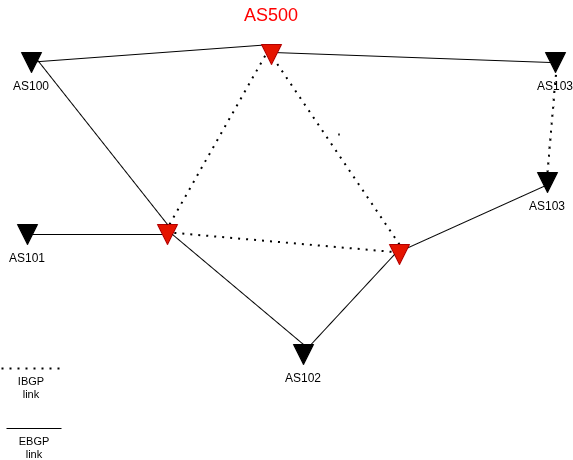
\includegraphics[width=0.7\linewidth]{bgp5.0.drawio.png}
    \caption{simple BGP network, showing both IBGP and EBGP links}
    \label{fig:diag5.0}
\end{figure}
% diagram shows two ASes with internal structure, ASBRs as edge nodes, links labelled as IBGP
% and EBGP.  one AS at least should have 3+ nodes to show the `mesh'
\subsection{Why does IBGP exist?}
IBGP is defined in the base specification for BGP, RFC4271\cite{rfc4271}.
IBGP has two roles in any AS which is part of a multiple-AS system - and it may
also be used for more general network architectures, though more often when BGP
is used as an `internal' network protocol, for example, in data-centre, many,
most or all BGP relations may be EBGP not IBGP, for reasons which will become
apparent shortly.  In this context, however, the topic is purely the usage of
IBGP, and EBGP, in the context of Internet routing (IDR).

One role of IBGP is to carry external routes between border routers in a
transit AS.  The routes exchanged are used both to enable actual forwarding
between ASBRs, and also to inform downstream external networks that those
forwarding paths are available.  Note that it is important to use BGP rather
than some other routing protocol for this role, because it is vital that every
attribute associated with a route is transparently conveyed across the AS,
subject only to specific intended changes to attributes.

\textbf{Figure \ref{fig:diag5.0} shows a simple BGP AS topology with both IBGP and EBGP links.}

Another role of IBGP is to provide some essential subset of external routing
that is required by routers and hosts located within an AS, in order to either
forward transit traffic or enable hosts within the AS to make contact with
external hosts. Unlike the first IBGP role, which must use BGP in order to
preserve exactly route attributes for re-advertisement, the internally
terminated BGP sessions could, in principle, be replaced by some other routing
protocol.  On occasion, and most often inadvisably, network managers may
'import' BGP routes into the IGP.  More often, and less obviously in poor
judgement, IGP routes may be imported into BGP.  However, this rarely makes
sense either, since in general EBGP is used to advertise larger route blocks
than an internal network deals in, so the actual `local' addresses of an AS are
more often written in BGP configuration as static values, for export to
external peers (over  \emph{EBGP}).  So in fact there are multiple overlapping
functional roles for IBGP:
\begin{enumerate}
	\item enable transit traffic forwarding
	\item enable BGP route transit re-advertisement
	\item enable internal host outbound optimal routing (but note that for most uses, internal host connections to external have no need at all of BGP - the IGP simply distributes a `default' route which ensures external ('internet') traffic is carried to the nearest border router.  BGP would only be required if a complex AS had a need to explicitly route externally addressed traffic via specific exit nodes. And, in this case, the larger question might be how to achieve the same effect for traffic in the reverse direction, a problem which IBGP alone cannot solve.)
\end{enumerate}

\textbf{Figure \ref{fig:diag5.1} shows a BGP AS topology with border routers (ASBR), and now also, core routers.
\footnote{There is a deliberate mistake in this diagram!  Not all ASBRs are directly connected - even though a path exists between them all, the unpeered ASBRs will not learn each other's routes.... (Unpeered core routers lead to different but equally catastrophic outcomes.)}}


\begin{figure}[H]
    \centering
    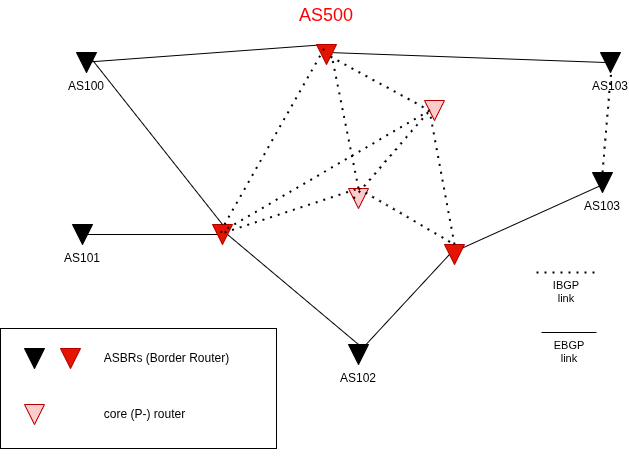
\includegraphics[width=0.7\linewidth]{bgp5.1.drawio.png}
    \caption{BGP network, showing ASBR and p-routers.}
    \label{fig:diag5.1}
\end{figure}

% {\color{blue} insert new diagram (2)}
% diagram shows an AS with ASBRs and P routers, the P routers are smaller.
% there should be a user-plane path through ASBR-P-P-ASBR,
% but only control plane links for all ASBR-P combinations
% Show the P router aggregate as `fabric'.

Note that the distinct functions of ASBR - to - p-router and ASBR - to - ASBR IBGP links enable respectively 1) transit traffic forwarding and 2) BGP route transit re-advertisement.

\subsubsection{Why and how does IBGP differ from EBGP?}
The important point is that, at the `wire level', IBGP and EBGP are almost
entirely identical.
There is just one visible distinction, which is that the route attribute \textbf{Local Preference} is \emph{always} present in IBGP Update messages, while for EBGP
\textbf{Local Preference} is \emph{never} present.
\footnote{Some, but not all, BGP speakers will disconnect a BGP session if this rule is broken.}
All other distinctions, while
absolutely vital, are observable only by observation of how routes received are
re-advertised differently or not re-advertised at all; there are two main IBGP
specific behaviours:
\begin{enumerate}
    \item IBGP re-advertisement does not extend the AS-PATH list attribute
    \item IBGP does not re-advertise routes to other internal peers that it learned from internal peers
\end{enumerate}

%%% {\color{blue} insert new diagram (3)}
%%% this seems a new and hard kind of diagram....
% show the updates at each stage - EBGP -(ASBR) - IBGP - (ASBR) - EBGP
% path attributes that change - LP added, AS path incremented

These two variations are really two sides of the same IBGP
principle/distinction, which is the suppression of the core BGP loop prevention
and path optimisation algorithm.  The consequence is extreme: it means that
IBGP \textit{cannot} independently operate as a routing protocol at all: there is no
mechanism in BGP itself to allow valid paths via internal nodes to be discovered.   Only when
every ASBR directly connected to every other ASBR, is it possible to avoid
having to use some additional IGP protocol to direct transit traffic.
This dependency on a second, IGP, routing protocol is not oversight, rather it
is fundamental to IBGP architecture, such that the IGP metric is explicitly
defined as an input into IBGP route selection.	To complete the explanation:
IBGP announces external routes and as part of the route announcement gives the
'next-hop' address for the egress node, where the next-hop address is known in
the IGP.  Thus, IBGP forwarding works by finding a forwarding path which would
be valid for packets addressed to the associated next hop.	As long as the IGP is
functioning correctly, then every intermediate node forward packets to the
correct ASBR using the following logic:

\begin{enumerate}
	\item first, lookup the internally reachable address (nexthop) associated with the destination external address, in the BGP table which is expected to be consistent across the AS, once the AS IBGP has converged for this route.
	\item use the IGP forwarding table to find the path to the internally reachable address (nexthop) found in step one.
	\item  forward packet using the path from step two.
\end{enumerate}

As long as the internal BGP tables all agree, the packet will follow the IGP
route prescribed toward the egress node's internal interface.
When the egress ASBR is reached, the ASBR uses its BGP derived forwarding table
to choose an external facing interface.  Note, the ASBR BGP route table mirrors
the internal ones except that at the ASBR the next-hop stored in the BGP table
is of the external peer.  The difference is because when the ASBR published the
route to IBGP is substituted the nexthop it received for its own internally
reachable address.  This change of nexthop is another typical aspect of IBGP at
a border node - however, change of next hop is a normal behaviour for BGP under
any circumstance of re-advertisement - it represents an instruction to direct
traffic \emph{through} the BGP router in question, rather than \emph{around	it}.

\subsubsection{fragility of IBGP, and the retirement in most ISPs of internal BGP speakers}

One critical point emerging from this description of IBGP function is the
importance of full BGP level connectivity between all traffic forwarding nodes
within an AS - it is essential that every internal node is (BGP) connected to
all ASBRs, because it is only from direct BGP peer sessions with ASBRs direct
that external routes can be learned.  Even one failed IBGP peer session leads
directly to high probability of lost packets, because the incompletely connected intermediate node
may still be on an IGP best path for some transit traffic - even when it does have a BGP session over
which to discover the nexthop for transit packets - so, any packets addressed to
routes currently served by the un-peered ASBR will not be forwarded correctly,
and therefore will be dropped, at risk otherwise of creating routing loops.

This fragility exists even if all ASBRs are directly connected, however having no intermediate internal nodes reduces the number of peering sessions required, and makes it easier to detect misconfiguration, which otherwise is subject to the vagaries of the IGP as to whether packet loss can occur.
This simplification is (one) goal of the introduction of MPLS in IDR.

However, one improvement in transit network architecture has at least simplified
the operation of transit networks by removing the need for `full-mesh IBGP' -
meaning, the requirement to distribute full route tables to all internal
routers in an AS.  The change is the introduction of MPLS as a transport layer
within an AS.  By converting internal routers to operate as MPLS label switches
rather than plain L3 forwarding systems, the responsibility for delivering
transit packets from ingress ASBR to egress ASBR has been moved from hop-by-hop
L3 address based forwarding, to an end-to-end predetermined path (`source
routed') concept.  In this case, the IGP is generally still used to setup MPLS
paths between ASBRs, with the possibility that specific traffic management may
be applied to optimise certain flows.  The ASBR function remains otherwise
largely unchanged: the main difference being that the forwarding plane logic at
the ingress ASBR, of selecting forwarding treatment based on the nexthop
advertised by the egress node, is enabled to be a MPLS forwarding rule rather
than simple L3 FIB lookup resulting in an egress interface.  Instead, the
egress interface specification includes an MPLS label stack, and that label
stack is assigned based on the IGP constructed MPLS path to the egress ASBR
nexthop.

{\color{blue} insert new diagram (4)}
% reuse the diagram with internal P routesr
% keep the routers, lose the IBGP
% draw in `tunnels' over the Ps

\subsubsection{Route Reflection}
Route Reflection is relevant in this thesis context for two rather distinct
reasons:
\begin{enumerate}
	\item it could contribute a technical aspect to a concrete implementation of PIR
	\item it illuminates some general aspects of attempts to extend BGP
\end{enumerate}

In brief - BGP Route Reflection (RFC4456) is well described by the full title
of the RFC: \textbf{\textit{BGP Route Reflection: An Alternative to Full Mesh Internal BGP
(IBGP)}}.

\paragraph{Route Reflection}
 (BGP-RR) is an extension to IBGP behaviour which allows
specific IBGP speakers to readvertise routes within an AS. BGP-RR adds two new
types of Route Attribute, including a list structure analogous to the external
AS PATH used in EBGP.  BGP-RR defines new rules on readvertisement of routes,
differentiating between regular IBGP clients and peer BGP-RR speakers.  An
important property of the BGP-RR design is that the regular IBGP clients do
not need to understand BGP-RR, and so gradual and non-disruptive transition to
use of BGP-RR is made possible.  The lesson from BGP-RR for a prospective
extension of IBGP is that even rather small change in IBGP principles required
significant changes in both the BGP protocol, and in the rules that govern it,
but was possible in a way which did not require change to the existing deployed
system software (but doe require configuration change, albeit mostly just
simplification).

% {\color{blue} insert new diagram (5)}

\begin{figure}[H]
    \centering 
    \begin{subfigure}{0.48\textwidth}
        \centering
        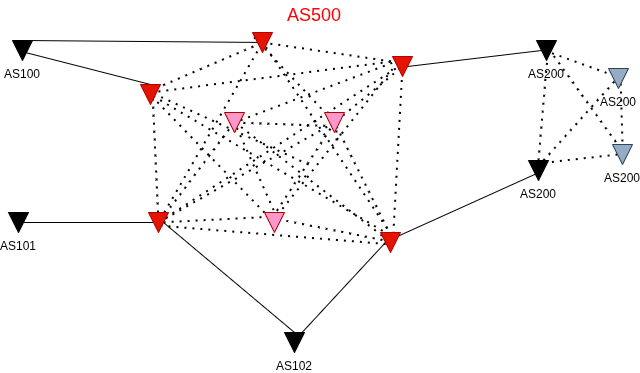
\includegraphics[width=\linewidth]{bgp5.2.a.png} 
        \caption{Before Route Reflection}
        \label{fig:Before Route Reflection}
    \end{subfigure}
    \hfill 
    \begin{subfigure}{0.48\textwidth}
        \centering
        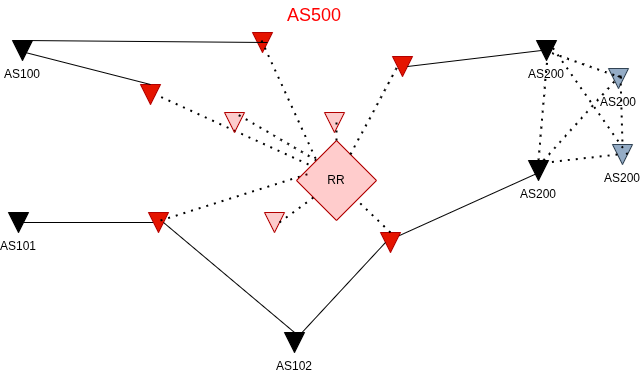
\includegraphics[width=\linewidth]{bgp5.2.png} 
        \caption{With Route Reflection}
        \label{fig:With Route Reflection}
    \end{subfigure}

    \caption{Route Reflection - Before and After}
    \label{fig:Route Reflection}
\end{figure}
% images/bgp5.2.png images/bgp5.2.a.png

% the RR digarm is a bit `stock'
% draw a before and after, with reduced number of links
% note in this fig - `note that RR breaks the no BGP between `P' router rule...

BGP-RR is highly relevant to PIR, if only because it represents the first
generally accepted change to BGP in the direction of centralised control.
However, perhaps a reason that BGP-RR found ready acceptance is that it is very
carefully designed to exclude the concept that a BGP Route Reflector should do
anything more than provide a transparent aggregation function for peering
sessions, in order simply to enable better scalability in a regular BGP AS.

\emph{A good question might be:} how is it that a `centralised controller' such
as a BGP Route Reflector, cannot easily be adapted to become a more directive
and prescriptive actor, rather than a passive tool?  A short answer is that the
crucial role in route selection in standard IBGP is performed only at route
ingress, which is to say, in the calculation of Local Preference.
As RFC4456 says, in Section10:
\begin{myquote}
	10 Implementation Considerations

	Care should be taken to make sure that none of the BGP path
	attributes defined above can be modified through configuration when
	exchanging internal routing information between RRs and Clients and
	Non-Clients.  Their modification could potentially result in routing
	loops.

	In addition, when a RR reflects a route, it SHOULD NOT modify the
	following path attributes: NEXT\_HOP, AS\_PATH, LOCAL\_PREF, and MED.
	Their modification could potentially result in routing loops.

\end{myquote}

And since BGP speakers receiving internal routes are similarly constrained - 
in RFC4271:
\begin{myquote}
	9.1.1.  Phase 1: Calculation of Degree of Preference

	....
	If the route is learned from an internal peer, either the value of
	the LOCAL\_PREF attribute is taken as the degree of preference, or
	the local system computes the degree of preference of the route
	based on pre-configured policy information.	\emph{Note that the latter
	may result in formation of persistent routing loops.}
	....

\end{myquote}

it is clear that the only point in an IBGP or IBGP+RR network for making policy
based evaluations of routes is at the ASBR entry point of a route.

\subsection{Standard IBGP}
In order to reason about modifying the behaviour of an IBGP network, it is
necessary to articulate its standard behaviour, with some focus on the ways in
which the interactions which underpin the collective behaviour of an IBGP mesh
work, and why it may be difficult to adapt the model to support concepts of
centralised or external control.  Here that is done(explained?).

An AS with more than one BGP speaker can be called an `(I)BGP mesh'.  In the
simple version of a BGP mesh, every border router is connected to every other
via BGP (of course, all routers in the AS are connected over actual network
links, and participate in some IGP, such as IS-IS or OSPF).  But critically,
every BGP speaker is \textit{BGP peered} directly with every other BGP speaker.

It should be obvious that every border router must be a BGP speaker, but less
obvious that internal routers should be.  However, in a simple BGP network
every router in the data-path for transit traffic must hold a full routing
table, and since carrying full route tables in other protocols - IGPs - is
known to be impractical, it means that every router must run BGP, otherwise the
internal routers will not have forwarding state for transit traffic.  This is
the classical hop-by-hop forwarding network architecture - modern networks
avoid the problem of having to run BGP on internal routers by tunnelling
traffic with MPLS.
But, for our analysis, we can disregard internal routers, on the assumption
that under either classical or MPLS modes, their forwarding paths can be managed
without impact, since they are controlled directly by the edge (ASBR) routers.

It is important to realise the critical importance of the integrity and completeness of the mesh, in the sense of every router being fully connected to every other, via BGP: just one missing link can lead to catastrophic misrouting.  This may appear to create a large number of potential single points of failure, at every link and interface in the mesh.  But there is an easy solution for this: as long as a functional IGP is in place, then BGP signalling traffic can always reach a mesh member unless it become completely disconnected.  The only requirement is that each BGP router uses an internal `loopback' address, rather than an interface address, for it's BGP sessions.  In this way, signalling of BGP can continue seamlessly under any amount of physical or layer 2 connectivity disruption.  

\subsubsection{IBGP - Core Principles}

The differentiated behaviours between IBGP and EBGP emerge directly from the core BGP specification in RFC4271:
\begin{enumerate}
	\item A BGP speaker identifies an internal (IBGP) peer simply by noting at the time of establishment of the peer session that the two peers share an identical AS number
	      % ( AS numbers are exchanged in the BGP session establishment messages)
	\item The AS path list attribute is not extended on routes sent to IBGP peers
	\item IBGP peers do not readvertise routes received from other IBGP peers
	\item IBGP peers on the AS edge use the route attribute Local Preference to inform their IBGP peers of the calculated `value' of a route
\end{enumerate}

\paragraph{IBGP Convergence}

An IBGP mesh operates on a distributed consensus principle: for every
destination prefix, one or more ASBRs may hold an advertised route from an
external peer - and the only goal of the IBGP mesh is to select just one of the offered
alternates, and ensure that the consensus selection is then adopted by all border
routers, including those that hold competing alternative routes.

The mechanism for reaching consensus and distributing the outcome is simple:
every ASBR receiving an external route directly evaluates the quality of the route, reducing the quality metric to a simple, single, linear value, which it then stores, as a persistent property of the route, in  its local RIB (AdjRIBIn (post-filter)); if at this ASBR there are multiple routes to the same destination prefix then only the best according to the Local Preference metric is eligible to be advertised internally; when a route is advertised \textit{internally}, then the first calculated metric is included as a path attribute named \textit{Local Preference}.

All other routers in the IBGP mesh will receive this advertised route, and possibly also
other routes, from other ASBRs, with alternatives for the same destination prefix(es).
As ASBRs receive routes from their IBGP peers, they do not re-evaluate them again, rather they trust that the received Local Preference is valid, and simply run the `Best Path' selection algorithm, which is weighted to rank Local Preference above all else.

Only if  there is a tiebreak for first place, based on Local Preference alone, do other considerations come into play:  there are some simple rules for deciding tiebreaks, which need not concern us
here.\footnote{It is possible in principle for a router within an AS to have arbitrary configuration rules which could result in a different outcome than were Local Preference to be followed.
	However, this is almost certain to be ineffective at best, and outright dangerous at worst, unless every router in the IBGP mesh has the same arbitrary rule.  But, this would be perverse - if the network operator wants to achieve a different result, then it is always better to do it by configuration at the route source.}

\paragraph{Route Diversity, Route Suppression and Best External}
In this way, the IBGP mesh rapidly settles on a consensus - which is made explicit by ASBRs withdrawing their own candidate routes for which
calculated Local Preference is not as good as the current AS-wide best; if the better route was already  known, then the ASBR should never broadcast the route into the IBGP mesh.
Therefore, many internal route advertisements are suppressed at source.

% Additional, once a best route has been accepted, other ASBRs may withdraw their
% own offers, leaving the current best as the only known route.
This behaviour aligns with `normal' BGP semantics, which dictate that a BGP
router only ever advertises routes which correspond to its own selected best route,
and therefore also the route which it uses for forwarding traffic.

However, this behaviour makes recovery from loss of the current AS-wide best slower,
because as the old best route is withdrawn, all alternates have to be again
advertised and a selection process performed, which might have several transient
states.  A popular optimisation is called `Best External'\cite{marques2012}, under which a BGP
speaker may advertise an external route which it `knows' is not best, and which
it does not itself use for forwarding.	This strategy ensures that when a
network wide best route is removed, the new best route may be more rapidly
selected over the whole network.

It's noteworthy that `Best External' enables a curiously perverse behaviour\footnote{Of announcing a route which it does not itself install in its local FIB} for a BGP speaker with forwarding capabilities, and in doing so illustrates some valuable lessons for would be innovators in BGP architecture:
\begin{itemize}
	\item BGP implementer at least are not averse to breaking-all-of-the-rules, when it suits them, when there is  reasonable confidence that the effect is benign
	\item BGP users are also not averse to using BGP modifications, as long as they believe the consequences are not catastrophic
	\item perhaps one reason that `Best External' has not been strongly opposed is that it is a purely internal (IBGP) tweak
	\item the reason that `Best External' is considered safe is precisely that the actual regulation of IBGP behaviour which makes it safe - i.e. rigid adherence to the IBGP consensus mechanism, which demands strict adherence to all of the IBGP specific procedures and constraints - is rigidly enforced.
	\item in spite of wide stakeholder acceptance, up to the level of implementation and use, in the end IETF was unwilling to endorse it; although a standards track product of IDR WG, it is now no more than an expired draft RFC
\end{itemize}
So, a useful and provably safe extension to IBGP has a strong prospect of adoption and implementation by the active stakeholders, if rather lower prospect of endorsement in IETF.  Key properties for acceptance are probably evident safety, and simplicity.  The fact that it could be turned on incrementally, and off very quickly, is also powerful reassurance for cautious adopters.\footnote{The fact that earlier versions of BGP4\cite{rfc1771} specified this behaviour may also help its case}

\paragraph{AddPath and Route Diversity}

\textbf{Advertisement of Multiple Paths in BGP (RFC7911) ('ADDPATH')} \cite{rfc7911} is at once hugely impactful for BGP implementations, and yet also rather trivial.

The major impact is on the low level encoding of a BGP message - for peer sessions that apply ADDPATH, the wire-format representation of prefixes - `NLRI' -  is transformed in a way incompatible with classical BGP.  In classical BGP IPv4 Prefixes are between 1 and 5 bytes in size, and their actual size is encoded implicitly in the first byte, so no delineation between prefixes in a list is required, in spite of their variable size.

In contrast, under ADDPATH operations, the 1 to 5 byte size of a prefix increases to the range 5 to 9 bytes, because a new `PathID' is attached to each individual prefix.  Even though, in most cases, a block of prefixes with a common path could in principle `share' the same PathId, it's entirely possible that in certain cases the PathId's would diverge, hence the requirement to add the PathID element to every prefix, not just every route  - even though PathID is assigned locally by the BGP peer originating the announcement, and has purely local significance to the peer session on which they are carried.  Thus, an implementation of ADDPATH must implement and selectively enable a variant parser and deparser for NLRI in ADDPATH mode (similar considerations to the IPv4 case also apply to IPv6 and other address families.  There is a practical first impact of this aspect of ADDPATH, which is that the bandwidth requirement for ADDPATH enable BGP signalling traffic can be expected to nearly double, even if only announcing just one route per prefix.

A second major impact of ADDPATH on BGP implementations is that the rules for keeping track of routes in the RIB (AdjRIBIn and LocRib) change, if only subtly.  If the `BestPath' selection process is ignored for the moment, the only change due to ADDPATH is that the extended prefix should be treated as the new key - so two routes with the same prefix, but differing PathId, should be treated as different `prefixes'.  This means for example that the rules for replacement and withdrawal of entries in AdjRIBIn and LocRib are working using the extended forms for the purpose of identity.

However, when it comes to selecting BestPath, then, for a given destination prefix, all routes to a prefix, must be considered. regardless of PathID, including also those with no PathId  at all(recall, ADDPATH is enabled per peer, so there may be a mixture of ADDPATH and non-ADDPATH prefixes in LocRib.)  And, if a chosen path is one received adorned with a PathId, it makes no difference to the way that the subsequent route processing functions than if a plain route is chosen.

When it comes to advertising routes the case is also not so complex - it is \textit{compliant} to simply readvertise only the single route which is overall best, in which case the observable distinction is only that towards peers enable for AddPath encoded transmission, the route would be attached to a prefix with some arbitrary PathId, which need only ever be the same in every case.

A different behaviour arises only if the BGP speaker is configured to send multiple routes, in which case additional routes must be distinguished from the best by use of some other PathID, though it matters not what PathId values are used, as long as all are distinct.

\subparagraph{How is the impact of ADDPATH trivial?}
The answer is that, for a receiver of AddPath diverse routes, AddPath is no more complex to manage  than is BestExternal - the important point is that in spite of their being a wider range of routes in view, the same rule for selecting best is still applicable, and must be aligned between the originators of the routes in IBGP and the receivers.  So, although other routes may be sent, there is no room for ambiguity as to which is valid.  The sole function of sending more than a single route is to allow that if and when the primary is withdrawn - explicitly, by use of the prefix, and it's PathId - then, a secondary route from the same IBGP peer is immediately available as a candidate for the new best route.\footnote{This is not intended as a in depth analysis of the use-cases for Add-Path.  One use is for Route Reflection, to enable RR clients to choose routes based on IGP metric, rather than have the RR attempt to do so.  The other is to pre-populate the best backup path in forwarding hardware, when that alternate route is announced by the same source as the primary (again, most likely a Route Reflector).  The `pre-programmed backup path' explains why simply replacing one route with another is not as effective as first advertising the secondary, before withdrawing the primary.}

\subparagraph{Why is ADDPATH significant in this context?} - because `PIR', the BGP Protection application developed for this project, uses ADDPATH as a solution to gaining visibility to alternate routes that may be `better' than the routes selected by ASBRs as primary routes.

\paragraph{IBGP Loop Prevention}

The principle  \textit{IBGP peers do not readvertise routes received from other IBGP peers}
is not entirely intuitive, and is sometimes described as `loop prevention', which is true but not as simple as the following
% diagram and
explanation illustrate:

% {\color{blue} insert new diagram (6?)}
% obvious diagram, a lot like some of the earlier ones

In standard IBGP (pre-Route Reflector), every ASBR links every other ASBR, and since external routes can only be injected at an ASBR, it's rather obvious that ASBRs would only need to listen to other ASBRs.  Moreover, the only reason that an internal, non-ASBR router (a `P' router) should need a BGP route table at all is in order to forward traffic, based on routes learned from ASBRs.  So clearly, `P' routers can have nothing of interest for an ASBR to learn. \footnote{in principle, there may be some AS internal routes wanted in BGP, but injecting them at a `P' router is in general perverse, since any ASBR will do, and making a `P' router an essential source of important routes would be an unnecessary source of additional failure modes.} Hence the rule \textit{IBGP peers do not readvertise routes received from other IBGP peers} is really a statement that `P' routers are only ever route-receivers, which is perfectly sensible.  The fact that it also prevents route-loops is almost incidental.

\subsubsection{Corollaries, Caveats}
Border routers, and all BGP routers, have high levels of autonomy - for example,
it is possible to write configuration rules that prevent an IBGP from accepting
any particular route, for example, one BR in an IBGP mesh could arbitrarily
`reject' routes from some other specific IBGP peer.  Whether this would be `useful'
is doubtful - but the resulting damage would be purely local to the perverse
router's externally connected clients.

More concerning might be the capability for a border router to `overstate' a
route it
originates in the mesh - a badly configured router could very easily direct most or all
transit traffic to itself, by advertising all viable/known routes with a maximal
Local Preference.
This illustrates the point that, within an AS, a very high degree of trust is
required - the power to evaluate an external route is delegated entirely to the
edge router that first receives the route.
Therefore, in any practical BGP AS network it is usually assumed that every
border router applies the same policy in the evaluation of routes - the Local
Preference calculation.
Anything else would mean that the AS as a whole would behave inconsistently.

Note: applying \textit{the same policy} is not exactly the same as applying \textit{the same
rules} with the same outcome - for example, it would make very good sense to
prefer routes received over peer or customer links to routes received over
transit/provider links.
The same policy on different routers or different peers will produce different, but consistent outcomes.

Summarising,
\begin{myitemize}
	\item Local Preference will always dictate the outcome of all IBGP route selection;
	\item  Local Preference is calculated only once, at the point a route is received
	\item Local Preference calculation must be done in a consistently, based on business priorities, expressed as \textit{policy}, and applied at the point of entry to the network.
\end{myitemize}

Then, as long as the \textit{policy} expression is well-formed and effective, 
the network can operate entirely without central control, and this distribution
of responsibility for route evaluation provides for high levels of scalability
and resilience.

( The main issues for scalability being the degree of interconnection required,
however just as MPLS largely solved the problem of scale fore internal routers,
Route Reflectors solve it for edge routers, without changing the overall
architecture as far as the question of policy application is concerned. )

\subsubsection{Other IBGP Specifics}
IBGP usage has aspects not mentioned above which are essential to pragmatic operation of a Transit AS.  It's a curiosity of BGP that whilst the IETF specifications are in many ways detailed and complete, alone they cannot be used in isolation to understand or describe real world usage which is nonetheless so consistently embedded in operator practice.
Fortunately, other resources exist, which largely fill in the gaps between RFCs, and almost as usefully as filling gaps, act as sign-posts to RFCs, especially `informational RFCs.
Three important resource classes are:
\begin{itemize}
	\item industry forum presentations - especially, `NANOG'\footnote{North American Network Operator Group}
	\item publications of Regional Internet Registries RIRs
	\item leading vendor technical documentation and training material
\end{itemize}

For the purpose of succinctly explaining and validating the `missing' essential elements of IBGP, two NANOG presentations suffice well
\begin{itemize}
	\item BGP Communities: A Guide for Service Provider Networks (NANOG40, 2007) \footnote{https://archive.nanog.org/meetings/nanog40/presentations/BGPcommunities.pdf}
	\item BGP Techniques for Internet Service Providers (NANOG50, 2010)\footnote{https://archive.nanog.org/meetings/nanog50/presentations/Sunday/NANOG50.Talk33.NANOG50-BGP-Techniques.pdf}
\end{itemize}

The two essential `hidden' aspects of (transit network) IBGP are:
\begin{itemize}
	\item BGP policy configuration ('route maps')
	\item BGP communities
\end{itemize}

\paragraph{Side Note: BGP `Complexity'}

It is a frequently heard observation, or even complaint, that `BGP is \textit{so} complex': often it seems with the underlying message that `BGP is \textit{unnecessarily} complex'; and it seems often that the complaint is driven by the sight of the often very large and unstructured configuration files which are required to operate a transit network effectively.  But to the extent that the complaint is driven by the size and structure of configuration, it is surely misplaced: the problem, if there is one at all, lies not with BGP but with use that BGP is put to: no other routing system is even capable of performing the task that BGP performs; and to complain about the complexity of configuration is no more valid than complaining about the computer language in which a compiler is written, simply because the reader cannot understand easily how the compiler works.
The reader/complainer should surely go on a course to learn about compilation techniques, and then be sure to take a few months or more to learn well the implementation language (and perhaps a few other languages as well too), before believing that they are qualified to assess whether a particular compiler is `over complex'.

In the opinion of \underline{this reader} (of BGP configurations), the problem with BGP is not that it is too complex, rather that it is not sufficiently complex - programs written in assembly language are also often `too complex' - as well as entirely unportable - and lack of portability which is also a problem from which BGP configuration policy suffers.

\bigskip

\paragraph{We return now}
to the topic of the core use-cases in IBGP for `route maps' and BGP communities, whereby hopefully some of the aversion to BGP complexity may be dispelled, with the benefit of understanding the motivation.

The background to this section can be found in either the `academic' track, or IETF track:

The academic track starts at Gao and Rexford's seminal work, "Stable Internet Routing Without Global Coordination" \cite{gao2000}(2000), and a second paper by Gao, "On inferring autonomous system relationships in the Internet"\cite{gao2001b}(2001), introduced to the wider world the expression "valley free routing", although the concept is deeply embedded yet never used in the first more theoretical paper.   There follows a great volume of subsequent academic work on the topic.  ( The more recent paper \fullcite{shao2021} is an excellent and up-to-date and rigorous treatment of much what follows here.)

In the IETF track RFCs 7454\cite{rfc7454} and 7908\cite{rfc7908} provide more practical perspectives.  However, Gao and Rexford's paper alone is sufficient to immediately understand and apply the basic principles described here, and their terms can be used directly:

\subparagraph{Problem statement}
A transit ISP  - indeed any Internet connected AS network - can cause instability , service failures and fatal loss of revenue or unwanted costs - if it fails to limit the traffic which it receives.  The mechanism to prevent this class of failure is simple: received routes must be very selectively readvertised - if in doubt, leave it out".  In particular, do not allow networks which are not `customers' to send traffic to destinations which are not themselves `customers'.

There are some parallels with the EBGP/IBGP dichotomy in this, however rather than two classes of entity, there are three:
\begin{myitemize}
	\item customer
	\item peer
	\item provider
\end{myitemize}
and there is no `built-in' rule which allows the rule to be embedded in software, nor is there a `built-in' rule which enables a peer relationship to be inferred.  But the mechanism described here is an analogue of the built-in rules for EBGP/IBGP.
\subparagraph{Valley-free routing: the canonical solution}
(Hereafter, \textit{Valley-free routing} is shortened to VFR.)

Route processing rules for VFR are defined separately for ingress nodes, that is, for ASBRs which receive routes from external BGP neighbours, and for egress nodes, which are also ASBRs, but working as route originators rather than as route receivers.
\footnote{It may seem obvious that an ASBR should apply locally the same readvertisement restrictions on EBGP re-export as its IBGP peer would, but that behaviour is not automatically applied for the mechanism described here.  It's a valid criticism of the low-level basis of implementing policy in BGP.

	% the issue here is an anlogue of the hard corner-case where multiple routes received at a single ASBR upset an otherwise simple mecahnism for optimising route selection
	The problem is this: the selective export rules at an ASBR are triggered by the presence of route attributes (Communities) added at the ingress ASBR.  But, at the ingress ASBR, if route export is based on the communities present in the route as received, then the rules will not be applied.  It's problematic in some BGP implementations, and it is not unknown to find parallel configuration blocks which apply the same logic to local (EBGP) route readvertisement and readvertisement of IBGP routes, in order to achieve the `obvious' intention of a single policy.  Even if the BGP implementation does provide a workaround, it's also possible that a less experienced network engineer may make the mistake of not understanding that such a problem exists.}

The rules are:
\begin{description}
	\item[ingress node] The ingress node role is classification and marking.  The principle is simple: every external peer is statically categorised as exactly one of:
		\begin{itemize}
			\item customer
			\item peer
			\item provider
		\end{itemize}
		The classification of a route is simply the classification of the peer that originated it - based on some static list.

		In the simple case three (mutually exclusive use) communities may be defined, though only two are needed, since the absence of either of the others implies the third.  For example, since customer routes are generally `always' re-advertised, they need not be explicitly marked, as long as the others always are.
	\item[egress node] At the egress, the action taken depends on both the classification of the prospective recipient of a route,and, for each route, the classification of the route originator.  There is a simple decision table:

		\begin{tabular}{ |p{2.5cm}|p{2.5cm}||p{2.5cm}|  }
			\hline
			% \multicolumn{4}{|c|} {}\\
			\hline
			Ingress Class & Egress Class & treatment   \\
			\hline
			Customer      & Customer     & readvertise \\
			Customer      & Peer         & readvertise \\
			Customer      & Provider     & readvertise \\
			\hline
			Peer          & Customer     & readvertise \\
			Peer          & Peer         & drop        \\
			Peer          & Provider     & drop        \\
			\hline
			Provider      & Customer     & readvertise \\
			Provider      & Peer         & drop        \\
			Provider      & Provider     & drop        \\

			\hline
		\end{tabular}

\end{description}

But, there is a `problem' here!  The rules for readvertising seem to be identical between Provider and Peer!  So, the simple table is insufficient - a priority rule is needed.  For example, when advertising to a customer, this table allows that routes from any source are admissible - but the best option is based on the ordering Customer $>$ Peer $>$ Provider.

In reality, there is often more complexity to the policies applied than described here, which is perhaps one reason why it is not useful to consider embedding more rules into fixed function software than the IBGP/EBGP functional split.

Moreover, customer/provider/peer classification is used for more than just the readvertisement at egress policy - for example, it is good practice to police rigorously what routes are even accepted at ingress from a customer, and also to some degree what routes are accepted from a peer.

But however complex, the principles are simple and stable - classify at ingress, apply policy at egress.

The final observation is this:

why is it even needed to use this explicit expression, especially in the matter of prioritisation, when BGP has `shortest-path/distance metric' path selection algorithms built in?
The main answer is that the customer/peer/provider rules are mostly about service and revenue protection - even if the expected outcome of default BGP might most often provide that same outcome, it cannot be trusted to do so.

The reason that default BGP rules cannot be trusted are manifold - two simple ones are:
\begin{enumerate}
	\item connected peers might try and game the system - direct traffic via `our' network, in order not to pay a transit provider
	\item ISPs typically `game' the AS-path length mechanism by selectively extending AS-paths ('prepending'), for what may be legitimate reasons.  But, it means in general that AS-path length alone is not to be relied upon as a guarantor of another ISPs commercial interests.
\end{enumerate}

But, there is also a hidden complexity in the intersection between default IBGP path selection rules, and community enforced constraints - it is this:

At an egress node a path may be ineligible for announcement, due to customer/peer/provider rules - but the AS-wide selected path - converged on as a result of AS wide Local Preference assignments - might not be the only one received in the AS.  So for the egress node in question, there could be a theoretical route available, but it is inaccessible, because there is a mismatch between policy expressed in the community/route-map domain, and policy expressed in the Local Preference domain.

Of course, in a well-formed aggregate AS configuration scheme, care is taken to ensure that this type of inconsistency does not happen - because, if it does, traffic may be black-holed, or at the very least, routed in a highly suboptimal path.

The conclusion is clear - policy expressed as low level rules without a high-level - probably automated - coordination design, are rather fragile, and can easily result in hard-to-diagnose problems

But, in the alternate world of fully automated configuration schema management, fixing problems locally, applying ad hoc fixes to local configuration files, risks both causing other problems, and also fixes being lost, when the configuration automation system refreshes configurations - or, if the configuration automation system allows manual overrides to be retained, risks perpetuating fixes for problems that no longer exist.

\footnote{'Peer' is more naturally used than (adjacent) neighbour, however in the specific VFR context `peer' has a quite distinct meaning, hence the localised use here instead of `neighbour'.)}

\subsection{IBGP - Conclusions}
The foregoing section sets out the context for experiments in using IBGP to solve new problems, or old problems in new ways, or attempts to modify IBGP to solve those problems.

There are examples of approaches which
\begin{itemize}
	\item use BGP protocol and existing BGP unmodified implementations to achieve important results - the Valley-free routing policy, based on BGP communities and route-maps
	\item changes to BGP implementation (but not the protocol) - Best External
	\item changes to BGP protocol - Route Reflectors
\end{itemize}
collectively, these represent the main `solution-space' which will be explored later, in support of the objectives which are described in part in the next section - \textit{BGP+SDN - A Thought Experiment}.
\clearpage

\section{BGP+SDN - A Thought Experiment}

\subsection{Prologue}

A network engineer in an ISP, looking into the routing state of one of their
border routers, sees a route advertised by a connected neighbour AS.  Perhaps
the route is `best' on this ASBR, and perhaps it is best for the entire AS, or
some partition of it.  Or not.	But, the route has caught the attention of the
engineer - perhaps because it is a route which handles some very large
proportion of their customer traffic, or at least, some important route as far
as the ISP customers are concerned, and therefore also of concern for the ISP, and the engineer.
Or maybe, the route being a /4, he wonders if it is not a `mistake'.

What now can the engineer do about this?

\subparagraph{If the route has been selected already as Best Path}
then, traffic may be flowing - and if the ISP has
a rather good network monitoring system - perhaps using(netFlow, sFlow, IPFIX,
(SNMP?)) - or `DPI' - then in principle the engineer could uncover some
'health' metrics for the flow in question - though obviously, port statistics alone
hardly help.  If a very smart network monitoring system, it might even be
possible to estimate round-trip-time, or packet loss ratios.  More useful still
might be to have historical data for the traffic to this route, for comparison
with current - even more useful might be to know, in the recent past, which
routes (paths, neighbours, ports) had been selected for this destination, and
whether there were any correlation between the paths selected and the
performance, as measured by this `very good monitoring system.

This being 2026, the engineer is no longer a human but an AI, and at least some
of the very useful monitoring and historical data is stored in some `data
lake'.
Still, the question is: what can the engineer do about this?

\subparagraph{In the alternate case where the route is\textit{ not selected}} - even though, the neighbour
peer is reliable, and the link is not congested, and, were it selected it might
be rather a good choice.  Sidestepping the obvious point here, i.e.: if it is
such a good choice, why does policy not already prefer it? (There can be good
reasons for this, e.g. path length variations due to variably applied
prepending.)  So, the engineer might decide to do some kind of selective `ping'
or `trace route', using the advertised route, even though the routing state in
his/her network makes it rather difficult - perhaps the ASBR has some special
feature enabling it, or some combination of MPLS and policy routing allows this
kind of experiment.  Since this network is evidently rather smart, perhaps it
can also report back to the engineer which peer connection then delivers the
return packets for this `route test'.  So, now, the engineer can see if this
alternate route is good, perhaps better that the existing route (of course, the
network monitoring system is also able to report on the current performance of
the route which is selected.)
Rather obviously, if the return path differs from the `correct' one, it is a
strong indicator that the route is probably not correct.

So, for this alternate case, though the question is the same as the first case
- armed with very good data about whether
an alternate route should be selected, or deselected, what can the engineer do
about this?

\subsection{SDN to the rescue?}
We might replace the engineer with a computer, saving money, and providing cover 365 days/year, /24hours/day - the computer never makes `trivial' mistakes, and can directly communicate over gRPC, netconf, YANG, http3, or even SNMP?.

Now the solution lies legitimately in the realm of `SDN'.
But still, there is a set of routers running BGP, choosing `optimal' routes in a distributed process.
While the routers may `speak' gRPC, netconf, YANG, it's insufficient for this task.
What is the method by which a router with a `good' route can enforce its peers that this route
should be trusted over the current best?  What is the method by which the
router announcing a questionable route can be directed to stop announcing it to its
peers?
At a protocol level the answer is simple, but only when the router announcing the route is the active party - the router with a better route can simply assert a higher
Local Preference, and similarly the bad route need only be withdrawn, or
advertised with lower preference.
So, the solution perhaps is simple: the novel SDN-BGP-CONTROLLER simply sends a message to the router with the good/bad route,
to request that the `route in question' should be assigned a different (lower,
or higher) Local Preference. IN other words, the router should selectively  outsource its
'tie-breaker' function to a third party.  But is this possible?

\subsection{SDN has limitations, any other options?}
At this stage, we might observe that if only routers were smarter, then this
outsourced Local Preference evaluation would not be needed...
But there is a problem with (building) very smart routers - which is that, they
need to react very quickly, even when 1,000s, or even 10s or 100s of thousands
of routes change.

But, this is good news, if only for SDN evangelists, because it means
that there is surely still a role for SDN...

\subsection{SDN V2.0?}
So now the issue is clearer - although SDN can detect the `problem', and perhaps,
calculate a solution, but, SDN alone cannot implement that solution.

What is needed is some kind of `modified' BGP router - modified only in so much that it
can be `properly controlled' by the `SDN controller'.  This next-gen BGP router
is obviously not `SDN' - it's just a router, designed as it should have been
since the start.  It implements some new control protocol, but nothing `smart'
- think `reverse-BMP'.

\subsection{Perhaps BGP could be the new control protocol?}
Working on the premise that the missing piece of a solution is a protocol
to modify specific `BGP routes' located in some internal state of a BGP
router; or, more specifically, to change the outcome of the Local Preference
calculation in that router (and also noting that in future, it might be useful
to be able to modify other re-advertised route attributes than just Local Preference)...

If the solution requires a (new) protocol, then obviously,
even if the protocol is not `BGP', still, the currency of
the protocol is in large part BGP encoded route attributes.
The question now is:  are we designing just a protocol,
or a larger `architecture'
- and clearly, if required, the architecture should come first.

Put another way:, if the idea is simply to substitute a post-filter AdjRIBIn route for
another similar route, then whether the protocol is bgp or not is not the
issue, rather, how should the controller frame the context of the request for a
new route, and, how should the controlled router behave?
Important questions relate to how the controlled router should respond as
relevant local and peer router state changes.

One - simple - solution would be simple substitution - the pushed route would
simply replace/override the original (post-filter) route in AdjRIBIn, which is
pushed into tiebreak.

\subsection{Framing solutions based on route substitution directives}

It is easy to propose, at a high-level, a route substitution, which simply replaces the target routers route processing and filter logic at the level of a single route,
but the challenge is how to
define the relationship between an entry in the target router's `pre-filter AdjRIBIn' table, and a substitute outcome of filter application, and how to define the currency and
applicability of the substitution instruction.	There are some extreme cases:

either:
\begin{enumerate}
	\item  match on the precise route, i.e the entire set of route attributes (could be prefix specific, or not).
	\item  match on some `regex' over the route attributes
\end{enumerate}

and also either:
\begin{enumerate}
	\item  retain the override only as long as the specific matched route is in AdjRIBIn
	\item  retain the override indefinitely
\end{enumerate}

Another dimension: route source - the instruction is initially driven by a
route in a specific peer AdjRIBIn.  But. the instruction could reasonably be
intended as to apply to only the specific source, or to any source.

\subsection{A policy defined solution}

It's emerging how to solve this /define this:
The goal is to define a substitution rule, and so far the substituted value is
clear and concrete - mostly the important factor is the assignment of
Local Preference.  The `match rule' is less clear, but only in terms of scope.
This is open to the controller, but too specific a rule may become invalidated by a
trivial change.  The open question is how to define rules which are less
specific.  But, this can be left out of the protocol.  A controller could
choose to issue overrides which are entirely specific. Ambiguous or flexible
matches are also easily defined.
The ability to define `smart rules' would allow for transfer of `intelligence from controller to router.
A router could declare its level of smartness.

\subsection{SDN approach, summary}

The SDN approach requires some form of extended BGP protocol, which allows controlled routers to correlate their existing internal routing table state with override directives.  The reason is that when the controlled router state changes, the target router cannot afford to wait for the controller's next instruction.  We are not \textit{transferring} the core role of evaluating all routes to the controller, just asking the controller to be a source of `hints'.

It's an uncomfortable role for an SDN controller (and there are more challenges still to come...)
\bigskip
But, this is, as titled, only a \textit{thought experiment}.

\section{Implementing external control in IBGP}
\subsection{Implications for exerting control in a distributed IBGP mesh}
We could state the objective in terms of observable behaviour: which is that,
every Border Router evaluates routes based on some enhanced procedure, which
may be informed by external factors, historical data, deep analysis of offered
routes, ongoing network monitoring or probes.
A central part of the sentence is `every Border Router evaluates ...' - i.e. we
avoid the question of how an external agent can exert control by stating that
the responsibility for making `better' decisions is left where it currently
lies - at the edge router which receives a new route.
But, we only are describing the wanted observable behaviour.  And the reason to
do this is to duck the question of how another entity can insert itself into
the
IBGP mesh with the eventual desired effect, as if the border router itself
applied better policy.
\subsubsection{The Importance of (Being) Local Preference}
In classical IBGP networks, consensus is critical.  If ASBRs do not have common
routing state, then the network fails - a packet arriving at an exit node which
does not know that it \textit{is} the exit node will loop or be dropped.  An AS may be
partitioned by IGP based route metrics, but within a partition consistency is
essential.
In this classical architecture, convergence based on Local Preference is the
only mode of operation.
But, an alternate mode can be considered, in which the exit
node once selected at ingress cannot be overridden at the exit - this requires
a tunnelling architecture, which would allow an ingress node to deliver traffic
directly to a chosen egress point, with a defined treatment.
In such a network, convergence on a consensus route is not important.
More importantly, in such a network local preference is no longer central - an
edge node could reevaluate a route and arrive at a different result -
consistency does not matter, the value of local preference is in reducing the
load on other routers.	But, in order for this licence to be useful, other
routes must be exposed.  `Best External' is a good start.
But, this architecture has much more to offer than just Best External driven
reevaluation - once all exit nodes are selectable, another BGP entity can
advertise routes which target those egress nodes, safe in the knowledge that
the alternate paths are viable.

\subsubsection{Design Space}
to make an IBGP mesh behave differently, we might
\begin{enumerate}
	\item  make ASBRs smarter
	\item  work with BGP in some way to allow ASBRs to still be dumb, but somehow overall enable the AS to behave better, whilst still being a traditional IBGP system - which must mean some via some additional BGP speaker(s) with special properties.
	\item  change the architecture
\end{enumerate}

The thesis scope is not to replace BGP, either as IDR or as AS internal
protocol.
And options 1) and 2) are not so different - the distinction is as to whether a
controller can be made effective when limited to using only existing BGP
principles, or instead, define some more powerful scheme which can in effect
make ASBRs smarter, or at least, more tractable.

\subsection{Detailed Analysis Of Conflicts and Resolutions Between Classical IBGP and BGP Controllers}
This section is rather dense in its logic, and essays a rigorous exposition
which justifies the following statements:

\begin{myitemize}
	\item A BGP Controller can be formally defined in an analogous way to a BGP Remote Reflector, with capabilities which are a super-set of a BGP Route Reflector
	\item Neither IBGP nor IBGP + Route Reflection are expressive enough or compatible with a BGP Controller
	\item IBGP + BGP ADDPATH (RFC7911)\cite{rfc7911} provide more relevant expressivity, though still insufficient
	\item IBGP + BGP/MPLS VPN (RFC4364)\cite{rfc4364} provides complementary expressivity to IBGP + BGP ADDPATH, but is also insufficient, alone
	\item IBGP + BGP ADDPATH + BGP/MPLS VPN in combination are sufficient for BGP controller - but, no vendor is known to enable the combination in an viable way.
\end{myitemize}

\subsubsection{Definition of a BGP Controller}
A BGP controller is a system which exerts \emph{dynamic} control over the
routes advertised and implemented within an AS.  It does this by interacting
with ASBRs using BGP and current BGP extensions, or by other means.

\paragraph{Scope of a BGP Controller behaviour}

\begin{itemize}
	\item A BGP Controller cannot `invent' routes.

	\item An AS acting under influence of a BGP controller should not be distinguishable by its behaviour from an uncontrolled AS, other than by inference by observing better or dynamic policy (an example of dynamic policy would be that a route initially rejected or selected may later change status, without any corresponding external route state change).

	\item A BGP Controller may have levels of capability:
	      \begin{itemize}
		      \item The lowest level is purely reactive to specific received routes: when a EBGP peer route is received, changed, or withdrawn, the controlled network selects and advertises a route other than that which ASBR policy dictates. When a later change removes or updates the route which triggered a controller response, the controller must again react in order to exert control, otherwise the override associated with the route is removed.

		      \item  Higher level capabilities

		            \begin{itemize}
			            \item  a more capable BGP Controller may issue directives which are generic or persistent: this would have the effect of protecting the AS from trivial changes to a `bad' route, which otherwise would undo the protective instruction.
			            \item  Orthogonally, a more capable BGP Controller may issue directives which have explicit time limits, or may issue prophylactic directives to ASBRs other than the ASBR which received the trigger route.
		            \end{itemize}
	      \end{itemize}
\end{itemize}

\subsubsection{Policy Versus Configuration versus Dynamic Control}
Conventionally, when an ASBR, and/or an entire AS, receives a `route', it runs
'best path', and either switches to some new route, normally the route received
(but, see MED), or more often, makes no change.  Then, nothing more happens,
until again received external route state changes, at which point the selected
and advertised routes may also change, subject still to Best Path, which is the
concrete expression of the AS policy.
If a BGP controller is introduced then conceptually it interferes with `Best
Path', and therefore, when again a related route change occurs, it must again
directly oversee the response.	IN this scenario, a base \textit{policy} is
implemented as conventional static configuration is each ASBR, and the BGP
Controller in some manner interferes with the AS route selection, but ASBRs
policy is unchanged.  In this case we can understand that the ASBR control
mechanism is a `control plane' rather than `management plane' strategy.
Its important to state that the `smarter' control mechanism crosses a boundary
into configuration ('management plane') - because the ASBR is being give a
'rule' to apply, rather than simply a routing protocol item which affects the
intended behaviour, but which is not identifiable as anything other than
'another' route.  This distinction is central: there might be constructed some
hierarchy of persistence, but still the persistent management plane strategy is
qualitatively distinct for a routing protocol extension.

BGP controllers thus fall into three basic categories:
\begin{enumerate}
	\item The BGP controller uses only BGP and current BGP extensions
	\item The BGP controller uses BGP with customised BGP extensions
	\item The BGP controller uses methods other than BGP, possibly in conjunction with standardised BGP.
\end{enumerate}

Note: The expression `uses only BGP and current BGP extensions' is ambiguous:
one might propose a mechanism which is technically BGP, but not supported by
any known implementation of BGP, and might require behaviour which contradicts
'mandatory' rules for BGP.  For example, the `wire' messages might be entirely
valid BGP, but the aggregate usage undefined.  Therefore, there is a
sub-category, or sub-categories:

The BGP controller uses only BGP and current BGP extensions:
\begin{enumerate}
	\item  in ways consistent with specification and live implementations, such that the actual behaviour corresponds to the intent
	\item  in ways consistent with specification, but with no known implementation, or implementation behaving in the manner intended
	\item  in ways which contradict specification, or reasonable interpretations thereof, and have no known functional implementations.
\end{enumerate}

Orthogonal to these categories of compliance are categories which relate to
mode of operation:
\begin{enumerate}
	\item The BGP controller operates by promoting a received route in order to suppress another route which would otherwise be selected and advertised.
	\item The BGP controller operates by interacting only and directly with the ASBR which receives a route, in order to suppress that route.
\end{enumerate}

\section{Implementation Strategies}

In the hypothetical thought experiment, however complex the rationale for
overriding the default policy outcomes of route selection, the range of
pragmatic options remains very limited:
it is already accepted that at the AS level the main scope for changing AS
behaviour is limited to making a different selection from offered alternatives,
with variants such as specific modifications to routes readvertised, and
potential to advertise distinct routes, or distinctly modified route attributes
at a more granular level.

How then can a controller use existing BGP to achieve a desired outcome of
removing a particular route from selection, or, a more specific version of the
same thing, enforce that another specific received peer route is preferred and
re-advertised?

The question can be deconstructed into two aspects:

\begin{enumerate}
	\item the element of learning of both the unwanted and alternate route, to include also monitoring that both routes, and any potential later arriving better route, remain in view of the control agent
	\item instructing the ASBRs within the AS to promote the alternative route
\end{enumerate}

Note: there can be interaction between action and observation: for example, if
the mechanism for changing the advertised route results in information about
either the deprecated or alternate route becoming stale, then the solution is
incomplete, because there is then no mechanism to react when for example either
the alternate route, or the unwanted route, is removed.

Assuming for the moment that a reliable route monitoring system exists - then,
since the only control plane action available to any BGP speaker which can
impact routes advertised by another is itself to advertise a similar route
which might be chosen instead - the question reduces to what route, advertised
to what IBGP peers, can have the desired outcome?  Clearly, a copy of another
route to the same prefix can be advertised by an IBGP speaker, to some or all
other IBGP peers.  Such a route can be crafted such that it is guaranteed to be
treated as preferred, simply by using Local Preference, or, with equivalent
effect, some additional attribute, e.g. a specific community attribute, for
which the IBGP peers are consistently configure to process with high priority.
However, using Local Preference is preferred because the advertised value can
be adjusted finely so that some  foreseeable and desirable external route
changes may automatically override the override.

So, which IBGP peers should receive this `special' route? It would be desirable
if a minimal distribution list could be effective - it might seem that the only
way to effect the redirection would to send the new route to every ASBR - but,
depending on some AS specific configuration, it may be sufficient to send this
'fake' route to just the ASBR which received the `bad' route from an external
peer, because if doing so forces that ASBR to withdraw the unwanted route  from
advertisement to internal peers, then all remaining peers will simply fall back
to the next `best' route. If the objective is just that - use the second best
route - rather than some other than second best - then, this strategy works,
with just one caveat:
the second best route must not lie also with one of the peers of the same ASBR
as the bad route.

However, the corner case of preferred route and default best route ingressing
at the same peer needs more careful treatment.
There may be a simple twist
which can resolve this: which is to use \emph{EBGP|} as the control channel to
'boost' the alternate route.
This certainly overcomes the problem of how to
force an alternate route selection between two routes received at the same
ASBR.
But, it introduces, or highlights, a different problem, which is one concerning the monitoring channel for the controller.
If the monitoring channel is one such as `Best External', or ADDPATH, then these both
require IBGP peer connections, and have the unstated (and essential) merit, of
conveying not only the existence of alternate routes, but also the calculated
local preferences for them.
The Local Preference of every candidate route is needed in order to calculate
which alternate should be chosen, and with what enhanced Local Preference to
announce it.  Switching to EBGP alone would remove the knowledge about
calculated Local Preference.  But, even if every ASBR is `wired' to the
controller both for IBGP as a monitor channel, and EBGP as a control channel,
still, by installing an override alternate at an ASBR, the Local Preference may
become unavailable over IBGP, because the presence of the new route causes the
monitored routes to be removed in IBGP.  This is even more a problem than it
may seem: if the bad route disappears, then the controller ought to remove the
override, and then the bad route will simply reemerge in IBGP.

Note: in general, this pathological behaviour only arises in the case of an alternate route received at
the same ASBR as the bad default choice.
Note also: if IBGP is to be used as the monitor channel, then certainly either `Best External', or ADDPATH, must be configured - otherwise, the existence of any alternates cannot be discovered at all by the controller.
\subsection{Uses of ADDPATH, NextHop Peculiarities}
We have  observed that for many situations, sufficient route diversity is enabled if BestExternal is activated, to allow a IBGP located controller to receive alternate routes which can be used as a basis for preparing a viable alternative to draw traffic from a path which the controller has determined to be `bad'.

ADDPATH has ambiguous definition and implementations, likely driven by ambiguity of the intended use.  The primary objective of ADDPATH appears to be to aid route recovery when a previously preferred route is withdrawn.  Other use cases \footnote{see for example Cisco IOS XE IP Routing Configuration Guide - Chapter: BGP Additional Paths} include enabling of BGP multipath.  It is implied that the natural `home' for ADDPATH is the RouteReflector rather than an ASBR.   The main point about ADDPATH is that even if overlapping paths are advertised by a single router, unless the paths have distinct next-hops, then the only usable path is the one in the set having highest Local Preference. Some implementations, will only advertise more than one route via ADDPATH when the additional routes would have different next-hops; if the router in question configures `next-hop-self' for IBGP, then this clearly implies that multiple routes will not be advertised.

There is a configuration `tweak' which can render ADDPATH much more powerful, and has the potential to lift ADDPATH into a level of capability which can be very useful for the controller application envisaged here.  The tweak is to disable IBGP next-hop-self while enabling ADDPATH.  In general, in order to have a functioning IBGP forwarding plane, the next-hops advertised should be redistributed in the IBGP IGP, otherwise when an ASBR attempts to install the resulting route in its local FIB it may fail, or worse, install a route which does not resolve to the correct ASBR.

However, this problem can be avoided by only selectively enabling both ADDPATH and simultaneously disabling `next hop self' for BGP peer sessions to a controller.

The combined effect of this configuration strategy is, or should be, that, for normal IBGP sessions, i.e., to all other ASBRs, the `normal' IBGP behaviour is shown - next-hop is always an IBGP mesh internal address, and only the single best route is announced.  Meanwhile, the controller role BGP speaker receives multiple routes whenever they are available .

The last, and required, beneficial aspect of this external next-hop pass-through strategy is that it also enables the controller to issue an effective override route to this ASBR.  Without the external next-hop information, there would be no way for the controller to correctly override the target ASBRs locally preferred route.  But, armed with the correct external next-hop, the controller can  issue a route override which has the desired effect.

There is only one possible catch, which is this - depending on the ASBR router implementation, if it applies the policy of refusing to advertise more than one ADDPATH route per next-hop, then the effect of the override route installation will be the loss of the underlying route from the ADDPATH set, to be replaced by the new `copy' route - which if it happens, invalidates the entire scheme.
However, and at this point we are deep into vendor specifics - but, depending on the implementation, it may be possible  - the case can be rescued by writing an export filter for the (ADDPATH) controller peer session, which excludes the new `fake' route from the ADDPATH list, and thus re-enables announcement of the base route.

There are undoubtedly a large number of implementation dependencies in this strategy - but, were the strategy to be accepted as a `valid' use case, it is plausible at least that even non-conforming vendor implementations could be fixed, so that the scheme could be made functional
\subsection{BMP: An Alternate strategy for route monitoring}

In the previous section the use of IBGP as a control and monitoring channel
were explained: in many cases, a controller can successfully operate by
monitoring routes received over IBGP, and, when action is required, promoting an override alternate route, simply by readvertising an existing route from another ASBR peer, but with higher priority than that set by the source ASBR.
We saw that in the challenging corner case, where the preferred alternate is reached via the same ASBR as the unwanted route, then it may be difficult to exert override control, and even more difficult to reliably
monitor the relevant routes.

It is not clear that a widely applicable solution to this problem exists, with just these tools of regular IBGP.
However, there now exists an alternate scheme for reliably getting route information from a
BGP speaker: RFC7854 - BGP Monitoring Protocol (BMP).

BMP has evolved significantly during the period of this work.
The initial BMP RFC, RFC7854 \cite{Fernando2016}, published in 2016, provided only for monitoring of the `Adj-RIB-In' routing table in a BGP speaker.
In 2019 RFC8671 \cite{rfc8671} introduced support in BMP for reading Adj-RIB-Out, and in 2022 RFC 9069\cite{rfc9069} introduced BMP support for Loc-RIB.
These extensions are, or could be, significant for implementing a BGP controller,
not least because the `Adj-RIB-In' of RFC7854 is not guaranteed to provide calculated Local Preference.
Without Local Preference, a BGP controller is unable to assess route fitness, except by attempting to replicate
the calculation done by each ASBR, and the possibility that the calculation
result may not agree introduces great uncertainty as to effectiveness of a
controller, not to mention a very large additional implementation effort which
amounts to re-engineering the BGP policy language of every potential ASBR in
use.

Anecdotally, different early implementations of RFC7854 BMP varied as to whether
Local Preference was supported or not.\footnote{RFC7854 makes no mention of whether the Ad-RIB-In monitored is pre- or post-filter, nor does the expression Local Preference occur anywhere in the text.}
A BMP implementation does form part of this thesis, however at the time of work no available `software' BGP speaker supported BMP - the implementation was tested with a physical router (Juniper),
but neither the Juniper nor the Cisco virtual routers available for study supported BMP,
nor did any other open source router.
The tested BMP implementation on a physical router was able to provide Local Preference.

For this reason, the analysis of a BMP based approach here is purely
theoretical.

\subsubsection{Using BMP to Implement a BGP Controller}
In principle, a controller could use only BMP to monitor routes, however, doing
so requires that the AS wide route selection be inferred, whereas monitoring
the actual converged RIB by passive participation in the IBGP mesh is
considered to be a safer and simpler approach - it allows attention to be
focused on routes which are an actual threat, because selected, and also to
monitor the effectiveness of an intervention.  It means that the BMP role is

\begin{enumerate}
	\item to select alternate routes, when it is determined that they are required
	\item to reliably monitor the targeted and selected alternate routes for change
\end{enumerate}

Concurrently, IBGP is used
\begin{enumerate}
	\item as the control channel
	\item as the primary threat monitor channel
\end{enumerate}

\subsubsection{Can BMP help solve the same ASBR alternate corner case?}

In part, the answer to the questions of the section title is : yes.  It does so
by enabling reliable monitoring of both unwanted and alternate routes.
However, BMP is purely passive - it leaves open the issue of route override.
However, the part solution of using EBGP can now be fully utilised, since BMP
ensures reliable and continuous route visibility.

\subsection{Controller strategies - A conclusion?}
We have seen that basic IBGP can enable useful degrees of AS programmability,
using just Best External as the route monitoring channel, and IBGP based
directed readvertisement of alternate routes to suppress unfavourable routes.

Additionally, BGP Monitoring Protocol (BMP) can provide an additional solution
for an important corner-case which IBGP alone cannot address, but only by using
complex combinations of BMP, IBGP and EBGP, and also only with certain more
recent/advances BGP/BMP implementations.

However, the full scope of ambition includes other features:

\begin{enumerate}
	\item  dynamic change
	\item  granular control
\end{enumerate}

Moreover, another topic has yet to be addressed, or even explicitly raised, which is preventative control...

\subsection{More Granular Control, via MPLS}

Already mentioned in this chapter is the BGP feature "Advertisement of Multiple Paths in BGP" (RFC7911\cite{rfc7911} -  July 2016).

In conjunction with the RFC "Using BGP to Bind MPLS Labels to Address Prefixes" (RFC8277\cite{rfc8277} - October 2017), a radically different and more flexible IBGP forwarding system can be constructed., one which in the limit approaches the extreme fragmentation level described in the early theoretical section XXX?

The basic concept is as follows: following the concepts of BGP ADDPATH (RFC7911), an ASBR can advertise multiple routes concurrently, of which one is the generally preferred `best path' choice, having the highest Local Preference value at that ASBR. BGP ADDPATH capability enables more than one route to the same prefix may be advertised, and a new attribute (Path Identifier) is introduced to distinguish updates for different routes.
In isolation, ADDPATH is not easily motivated - it does not provide any explicit way in which an internal peer could directly utilise routes which are not `best', nor even `best' routes, in the event that the IBGP mesh has selected another egress router than the ASBR advertising a route with ADDPATH attributes.  Even the question of whether this is an EBGP or IBGP targeted capability is left unresolved in the RFC\footnote{A clue may be found in the original draft title for the RFC, which was "Best Practices for Advertisement of Multiple Paths in IBGP", and a related contemporaneous IETF draft: "Fast Connectivity Restoration Using BGP Add-path"}

RFC8277 explicitly describes use of MPLS next-hops with ADDPATH (see e.g. Section 2.2:
\begin{myquote}
	If the procedures of [RFC7911] are being used, a four-octet "path
	identifier" (as defined in Section 3 of [RFC7911]) is part of the
	NLRI and precedes the Length field.
\end{myquote}

This enables a direct forwarding path to be established, which guarantees that traffic directed into an MPLS tunnel at an ingress ASBR will be directed to the route source corresponding to the advertised path at the ASBR that advertised it using ADDPATH.  Without this capability,  traffic for the selected destination can never be forwarded other than via the AS wide route established by consensus between ASBRs.

Once the feasibility of the principle is established, the remaining task is to implement the feature in a way compatible with the objective of PIR / BGP control: however, the BGP aspect is rather simple: the BGP speaker which implements a controller function should negotiate the appropriate BGP capabilities which permit ADDPATH and MPLS next hops, and the ASBRs should be configured to send two or more paths per received route, where alternatives are received, to the controller role IBGP peer.  Now, the controller can always select an alternate route for the entire AS, by readvertising the MPLS route with uplifted local preference.  Of course, this still requires that all ASBRs support the explicit MPLS forwarding path, even if not ADDPATH.
Variations on the design can reduce the requirement for RFC8277 support by designating an internal MPLS forwarding point which installs a forwarding rule: for example, a BGP controller could integrate the MPLS forwarding plane logic required, on a `P' router adjacent to ASBRs.

There remains a very remote corner-case, which is the possibility that a large number of `bad' routes exist at a single ASBR, such that ADDPATH cannot reasonably be configured to propagate sufficient depth of alternatives than a hypothetical best path at the same ASBR can be obtained.  But it seems doubtful that this represents a serious obstacle to deploying a protection scheme using ADDPATH and MPLS - the more realistic concern is whether the additional complexity required to save the base corner case could be justified.  A simple deployment based on basic IBGP and BestExternal, or including BMP, seems a sensible first step for any deployment of PIR in a protective role.

However, if the use-case is the more general one of `More Granular Control', then ADDPATH+MPLS\_NEXTHOP are well-placed to make this a reality - the challenge then moves into the issue of how to create a coherent management system for a much more complex flow structure, and how to build a service concept which  can take advantage of this revolutionary capability.

\subsection{Dynamic Control, via vanilla BGP}
Even RFC4271 BGP provides that Local Preference may be reevaluated: see RFC4271, section 9.1.2:
\begin{myquote}
	If either the immediate next-hop \emph{or the IGP cost to the NEXT\_HOP (where the NEXT\_HOP is resolved through an IGP route) changes}, Phase 2 Route Selection MUST be performed again.
\end{myquote}

So, the IBGP based controller is at liberty to change its mind, or take its time making up its mind, or even try out an option, and revert if it does not work out - all the while behaving no differently to how a conventional BGP implementation might do.

The obstacle to dynamism is not in the protocol, or the architecture, but purely in the legacy policy implementations, which have no stateful model.  Of course, even the controller should take care to be able to remove a route rather quickly, when the route itself is withdrawn or changes at the ingress ASBR.

\subsection{Policy, Configuration or Protocol?}

The focus in this chapter so far has been on a protocol based strategy to adapt or extend the current IBGP architecture to enable novel behaviours, whilst protecting the essential elements of stability, scalability and performance which epitomise the existing architecture.

However, it may be that an adaptive, yet existing protocol based, approach is not the only possible solution, let alone the best.  In this section, other approaches are considered.  One alternate idea is to use configuration, or \textit{policy}, rather than signalling, to achieve the same high level goals; another is to extend the core protocol, or to graft on to it additional side channel protocols, analogous to other extensions.

\subsubsection{Terminology - `configuration' or `policy'?}
The terms \textit{configuration} and \textit{policy} overlap in some degree: if the term \textit{configuration} were to be used, objections might be that the term is inappropriate, or impossible to implement as device specific configuration, or simply that it causes confusion, while \textit{policy} could be seen as too abstract and ambiguous, and arguably is only a term for an abstract construct, which is eventually always embodied in some form of configuration.

For the purpose of this section, the term \textit{policy} is preferred -  but, it is understood to mean a concrete unambiguous set of `statements', which could, and probably should, be expressed in some DSL\footnote{Domain Specific Language}, which in some cases might simply be the native configuration language of the BGP speaker in question.

In other words, policy is independent of style of expression, and its domain is purely semantic rather than syntactic - and while a formal syntactic form might be desirable, formulation of policy need not wait on formulation of a perfect language in which to express it.

\medskip

As important as the question of policy encoding is the topic of policy dynamics and persistence, for example, if some policy directive is imposed, what then is its scope, in terms of lifetime?

But, if we allow that the policy language \textit{includes} a time related dimension, then the question of persistence can be moved into the policy ontology domain, just as we should expect that a policy directive can also include scope variations, for example `for all peers', or, `for all external peers'; so `until further notice', or, `until next system restart', or `until peer XXX BGP session restart' should be valid qualifiers on any policy directive.

\subsubsection{Explicit Control contrasted with Policy - An Example}
Suppose that a controller determines that some route -  a set of NLRIs with a common path attribute set - is to be deprecated, or entirely excluded from use and external re-advertisement - then, a `policy enabled' controller should send some directive consisting of some `match' term and some `action term'.

The action term is more easily conjectured - e.g.: `set Local Preference 10', or `filter from Adj-RIB-In'.

The match term could vary: it might simply identify prefix and the source external peer, or source adjacent AS: it might match the exactly advertised route prefix, or some subset, possibly as an LPM\footnote{Longest Prefix Match - i.e. where X.X.0.0/16 might be used to exclude several more specific prefixes, even if the actual prefix is not present.} match term.

At it's most specific, a match term might be written as some regular expression over the set of path attributes, or by reference to an ADDPATH Path Identifier.
\medskip

Immediately, it appears that \textit{policy} based control may in many ways be more flexible - and perhaps more useful(!?) - than any routing protocol based system.  That distinction can be made explicit by pointing out exactly the range of policy directives which can be `encoded' simply by using the route-override schema proposed in previous sections: which is to say, the low level action is simply to install a static route which may have higher Local Preference than another, and the time based dimension is `until further loss of peer session with controller'.

If the controller's continuing control is assumed then the semantics may be more specific, but difficult to define in some unambiguous language, unless the scope is limited to the single transaction of install route, then later withdraw it, if replacement itself changes,  or in any case, when the adverse route is withdrawn.  But even this cannot be expressed as policy, because at the policy target the replacement route may not be visible.

In conclusion, although a policy based route override may be superficially appealing, it doesn't seem possible to articulate even the simplest wanted control plane function directly as a (management plane) policy function.  The reason for this is not hard to find: only if the logic which governs the controller can be encoded in a policy directive, can a policy based system provide an equivalent capability to a controller based system.  Moreover, even if the policy language can define a rule which allows the target to behave exactly as a controller would require, it still would require that the target have also the same state visibility as a controller, to the extent that the policy relies on external state.  And, if the policy based expression was a useful long term `configuration', then a better strategy would be simply to use a controller to write policy based static configuration, and rely on an optimised, static, policy management strategy.  Arguably, that position simply represents the current, inadequate, state-of-the-art in IDR management.

\bigskip
In plain language, in answer to the question  "can route attacks be effectively mitigated simply by updating ASBR configurations faster, and with more granular structure?", the answer is a simple "no".
For example, the controller may use an ML analysis to identify a threat, but the analysis may not yield a simple policy rule other than an exact match for every attribute of the rejected path; or, the threat assessment may be based on an external metric - e.g. packet loss, or unexpected traceroute behaviour.  These \textit{cannot} be reduced to a policy language.  The best that could be hoped for is that the controller might, in some cases, be able to write some less specific policy rule which could avoid the ping-pong of threat route being trivially readvertised, then requiring to have the  rule rewritten,  By the controller; but this is at best an optimisation which is clearly not applicable in many cases, and offers no functional advantage.  A better way would be to use `smart' configuration to write those rules which might have long running applicability, and save the controller to handle the cases not addressable by configuration/policy.

\subsubsection{Control using Explicit Addpath Path Identifiers}
At the opposite end of the spectrum to \textit{policy} based control is the idea of extending ADDPATH to support control: when an ASBR advertises routes with ADDPATH, then each specific route gains some form of unique identity - such that it is conceivable that some protocol extension could use an ADDPATH route identifier to launch some further protocol interaction.

This concept appeals, because it potentially solves in a direct way the core challenge - to reject, or demote, a specific route - which can otherwise only be achieved indirectly, and rather inelegantly, by strategy that simply selects and advertises differently an existing route, which is clearly a `kludge' or workaround, rather than a natural extension of the existing architecture.

It is not possible/intended/practical to devote so much attention to this topic (Control via Addpath), although in principle it might be a very fruitful direction for future work, but a few further comments are still useful in the context of this Thesis/work:
earlier, the problem of improving resilience to routing attacks was divided into the separate problems of monitoring route state, mitigating threats, and managing mitigation as routing state changes.
In that context, ADDPATH is seen as a purely passive potential monitoring solution, ranked more widely effective than `Best External', and alongside, if not directly comparable with, BMP.

ADDPATH has no obvious advantages as a pure monitoring tool than BMP, and some disadvantages, i.e. not always can ADDPATH be relied upon to advertise potential alternates, and there is even a risk that a mitigation action could lead to loss of visibility of a required route, and thus disable ADDPATH based mitigation entirely in some cases.  However, if the Path Identifier attribute which ADDPATH adds to all routes, can also be used to target a route for demotion, then ADDPATH, or to be precise, the ADDPATH Path Identifier, could open up a possibility otherwise impossible, which is to target the `bad' route in some way, rather than just attempt to `drown out its voice', with some other route.  It's possible that the ADDPATH Path Identifier could be discoverable by BMP, as well as by listening directly to a BGP peer, however, that may not affect the outcome of asking `how can ADDPATH Path Identifier be used for direct mitigation?'.

One response to this question could be to draw on the strategy of ROA, which is a dynamic side channel that continually updates state in each ASBR, so that at `decision time', the local BGP system may rely on additional state - in case of ROA, the ROA:Valid/Invalid/Unknown condition, or for PIR-via-ADDPATH a similar, perhaps identically expressed state value: PathIdentifier:Valid/Invalid/Unknown.

One complexity for PIR compared to ROA is that, when the route is first seen, the related state can not yet exist - only after re-advertisement to an IBGP ADDPATH capable peer would the state value be resolvable based on an external agent input.  So, in the PIR case, and unlike ROA, the BGP decision logic needs to be re-run in the case that a PathIdentifier based external state is received.  But, this mirrors an ROA implementation challenge - if an ROA update is received, which affects an existing route, how or when should the BGP speaker reevaluate, and potentially change its best-path selection outcome?

For ROA it is credible, but sub-optimal, that the re-evaluation is deferred, or even never taken, while for ADDPATH driven clearly the revaluation is essential directly the ADDPATH control message arrives.  However, the prospects for easy implementation of such an extension seem good - there exists already in many BGP implementations some mechanism to enable such behaviour, and even the RPKI framework lends hope that a side-channel can be made effective.  Of course, changing BGP protocol itself is also an option...  but the examples of ROA/RPKI and BMP show that side channels can be easier to gain adoption than wholesale changes to the BGP protocol itself.

To sum up and review this candidate new approach:
the system can be quite `fail-safe' - it doesn't have the weakness of overloading and readvertising other routes, so when the adverse route is dropped, then the state returns immediately to `normal', rather than depending on a controller to discover the change and remove the advertised override;
fail-safe property is enhanced by the fact that if the `side channel session' is lost then immediately the control state can be removed, and again the system returns easily to default behaviour and state.
One can imagine further enhancements which make the solution even more powerful; if some or all new received routes are initially treated with very low preference, it would allow a more intrusive controller to engage and control route selection by selectively marking as valid some subset of routes, so if a highly attractive new route appears, the controller can swiftly elevate its preference, while protecting against possible short-lived interruption which is needed when working in a more passive/responsive mode.

One major disadvantage is that this would require substantial functional change to existing router software, albeit based largely on existing similar schemes for RPKI/ROA.

% \subsubsection{Comparison with, and Relevance of, ROA}
% ( In a later Section ROA is briefly described, refer to that section if ROA concepts are not familiar.)
% The relevance of ROA to this thesis is that

\section{ROA / RPKI}

ROA (Route Origin Authentication) forms a part of the set of recommendations, protocols and architecture which has as its head the RFC6480 ( An Infrastructure to Support Secure Internet Routing )  \cite{rfc6480}.  Most relevant for this context is the related RFC6811 ( BGP Prefix Origin Validation ) \cite{rfc6811}
The RFC were issued more than 10 years ago, and current BGP commercial implementations (2025) have mature support for ROA as described in the RFCs.  Some Open Source BGP implementations added support for ROA during or after the work on this Thesis.

Before briefly describing ROA, some words on the relevance to the Thesis:
ROA, and the RPKI/Secure Internet Routing program have near identical objectives to the Thesis - i.e., concrete, pragmatic solutions to Internet integrity threats.

Given the widespread adoption of ROA by all required contributors - router vendors, transit ISPs and AS number resource owners, there is in ROA a clear example of the kind of protocol and practice changes which the Internet community can and will approve and adopt.

In particular, the close attention given in ROA to gradual and uneven implementation, failsafe/fallback considerations, scalability, and performance, evidence the need to address those topics in any work which aspires to influence future IDR development.  The kernel of ROA is just a few hundred words in RFC6811, but the supporting infrastructure and ecosystem changes required cover multiple RFCs and far more complexity, than the actual BGP protocol behaviour changes.  If another program with similar scope to ROA is to be treated seriously, then the wider considerations of migration, stability etc must at least be acknowledged and addressed with sufficient rigour to give confidence that the approach has the prospect of being developed to the level of ROA/RPKI.

\subsection{ROA In Brief}
Without ROA, a BGP router may be configured - (or, equivalently,'policy defined') - to inspect the `origin AS' in every path it receives, and apply some validation logic ; the validation logic amounts to : for this advertised prefix, is it known what origin AS should be in the path?  IN other words -do a simple sanity check of prefix against a table of known ASes and owned prefixes.  Before ROA was introduced such checks could be configured, but only at the cost of rather large BGP configuration files, with a need to frequently update them (since there are over 70,000 AS numbers and the list of routed IPv4 prefixes is around 1,000,000, a complete table would be rather large ad very likely many BGP speakers would either not accept such a configuration, or work well if they did.)
ROA solves this problem of manual configuration efficiently: AS owners are provided with a mechanism ('RPKI') of asserting their `ownership' of prefixes, and more specifically, a mechanism of declaring precisely which prefixes can be validly advertised for a specific AS.  The mechanism of RPKI allows this table to be mirrored directly in any BGP speaker's internal state, as a new type of routing state object.  IT allows a BGP router to check for any path it receives whether or not, based purely on the prefixes and origin AS, if it appears to be valid.  Using ROA, a BGP speaker can determine for every path it receives which of three states are applicable, the states are:
\begin{itemize}
	\item Valid
	\item Invalid
	\item Unknown
\end{itemize}
What a BGP speaker should do with this additional data is not specified directly in RFC 6811 or in any other RFC, but the best treatment strategies are outlined, and are unsurprising
\begin{itemize}
	\item when a ROA entry exists for a route then all received routes can be only one of the two states, Valid or Invalid.  If both Valid and Invalid paths to the same prefix are received concurrently, then the local behaviour should always favour some Valid route, over any Invalid route.  The open question at both BGP speaker level and AS level is how to respond if \emph{only} Invalid paths are available: RFC6811 and related later RFCs, e.g. RFC7115 \cite{rfc7115} caution against rejecting entirely such routes.
	\item when NO ROA record exists for a route, the behaviour is no different to pre-ROA
\end{itemize}
There are some complexities in detail implementations, relating to routes and ROAs with different prefix lengths and overlap, however they don;'t affect the analysis which is relevant here.

This completes the needed standalone description of RFC6811/ROA, but the topic of ROA in the context of the Thesis also arises in an earlier section.

\section{IBGP Topologies}

IBGP and its attendant protocols and configuration schemes have a single simple purpose, which is to build a single logical router from a distributed set of routers (and links).

In RFC4271 BGP there is little flexibility in how this should be done, and the classical `full-mesh' IBGP was the only option available.  However, RFC4271 already contains the seeds of something more flexible.

Here, I outline the background
\medskip

\subsection{Separation of control-plane and forwarding plane in BGP, using Next-Hop Path Attribute}

A related property of BGP is its support for separation of control-plane and forwarding plane: this flexibility arises from the existence and usage of the `next-hop' attribute.  If a BGP speaker re-announces a route with the same next-hop as present in the route received, then that router effectively removes itself from the forwarding plane for traffic corresponding to that route.  The alternate strategy, `next-hop self', constrains the forwarding path to pass through the re-advertising router.  But  `next-hop self' is nothing more than convenient configuration shorthand for inserting a router local address, usually an interface address, into the route announcement.  The onus is on the BGP implementation, and the configuration, to ensure that the announced `next-hop' is valid: in principle, anything is permitted.

The flexibility of `next-hop' is wider than just this: VPN next hop flexibility is defined in RFC4569\cite{rfc4659} (2006), and RFC5549 (2009) \cite{rfc5549} specifies generic "Advertising IPv4 Network Layer Reachability Information with an IPv6 Next Hop"; moreover, the more recent  MPLS next-hop options have also already been mentioned: (RFC ??X, RFC ??y). (RFC5549 is now obsoleted by RFC8950, but the point is that in 2009 BGP next hop flexibility was already well accepted).

\medskip
Next-hop enables the separation of control and user plane in BGP, and the flexibility to set next-hop with different classes of `address' - where treatment might be a better term - enables a diversity of forwarding plane transports.

\bigskip

To return to the question, and refine it - what good does it do to delocalise the BGP termination, and therefore also the loci in the  control plane at which consolidation of routes, via a best-path selection process, is done?

The answer, if there is a positive one, is that it may afford the opportunity to break the monopoly on route selection held by the `dumb' edge routers, and relocate it into some `smart' BGP system.  And now it is clear that the block to doing that is that an ASBR must run best-path, in order to eliminate options which cannot be advertised, and because it must run best-path, it must also run the Local Preference evaluation algorithm.

But there is an unproven assumption in this chain of logic - which is that the ASBR must run Local Preference calculation itself, in order to run BestPath itself.  Is it possible that an ASBR could outsource Local Preference calculation, but in-source BestPath?

Or, could the ASBR outsource Local Preference calculation \textit{and} Best Path selection?

The answer in principle is yes - consider the case that the EBGP sessions are passed-through the ASBR onto some internal BGP speaker.  That internal BGP speaker is in the EBGP role with regard to external routes; and as such is in the best position possible to run some enhanced Local Preference calculation, and then the challenge switches to the locus for Best Path selection, and mechanisms for aligning the subsequently selected routes with the forwarding plane Edge Routers.

\medskip

Before taking up the challenge of designing a specific solution for this particular separation of control plane and user plane in BGP, it is appropriate to describe in more general terms the implicit topological structures of actual and potential BGP networks.

\subsection{One topological extreme - single central controller}
Because there is one extreme, which is the basis of for example early RCP work, under which all externally connect BGP peers have BGP sessions which terminate at the single central controller of an AS, reducing the ASBR and internal AS forwarding infrastructure to a pure fabric or IP level cross-connect.  In this architecture, the internal forwarding state and its management can be anything we choose - it could be end-to-end OpenFlow, with one million or more flow rules per interface in every `ASBR', forwarding with e.g. hop-by-hop MPLS, or based on a pure L2 forwarding domain.  In such an architecture, we could envisage the highly granular service model entailed by "BGP Egress Peer Engineering" being `easily' enabled by assigning specific L2 addresses per egress port than egress node.

This is not a serious proposition, of course.  The resulting L2 network is probably close to the worst possible design available, simply moving the responsibility for optimising flows onto a simplistic protocol whose flaws and limitations are well enough known not to need repeating here\footnote{i.e., IEEE802.1d Ethernet Spanning Tree or descendants}.  A better term than `moving responsibility night be `abdicating responsibility'.

However, while keeping exactly the external control plane design we could migrate to something better - for example, the MPLS-SR (Source Route) scheme can clearly provide the function, the challenges being, one expects, performance of the control plane - and the lack of a candidate for the controller.

An important question for either the hypothetical, simplistic, L2 solution for centralised control, or the futuristic MPLS-SR, is how to provide a performant and reliable channel to install forwarding state - the actual forwarding semantics are less of a challenge, and there is a clear spectrum of forwarding semantics, from the simplest case - AS-wide, single path per port, though IGP partitioned (hot-potato), through to explicit per-prefix, port-to-port, granularity, aka RFC9087, `Segment Routing Centralized BGP Egress Peer Engineering'\cite{rfc9087}.

Since we are only here describing models, we could pass-over the obvious observation that, just as OpenFlow is probably not the best choice, regardless of which fabric tunnel forwarding mode we might choose, some form of BGP clearly is a right choice, and in reality, if the problem is exactly and no more than installing pre-calculated flows in ASBRs, the only choice - it is hard to argue that anything good enough would be materially different than BGP.  But note, in this case the BGP is entirely without any complexity of best-path selection - it is simply a very dumb ASBR doing exactly what it is told, no more, no less.   We could also note that any optimisation such as `Fast Reroute' can simply be delegated to the forwarding fabric rather than the edge-to-edge forwarding state manager.

\subsection{The opposite topological extreme - BGP Instance per external port}

In the previously described, and opposing, topologically extreme model, every EBGP BGP peering TCP session is transparently forwarded by ASBRs, to a central point.

In this counter extreme, every EBGP peer terminates at its own single instance of BGP, located in the ASBR it attaches - to be clear, this means that a single physical router hosts \textit{many} independent BGP instances, with the result that, within the AS IBGP mesh, there are exactly as many `logical ASBR's' as there are external BGP neighbours.

It is already known that above a certain size of AS there can be a scale problem, and in this extreme topology the scale problem will inevitably be even more impactful.  However, there are also well tested  mitigations to this scaling challenge, in the form of Route Reflectors, or Confederations, so the proposition may not be so impractical as it seems at first glance.

Perhaps the first question arising from this design is:  is this topology model materially distinct from  conventional BGP?  The answer depends on a so far unaddressed issue\footnote{no pun intended}, which is, how are these independent virtual BGP instances to encode their next-hop, which is what must be used in order to enable forwarding to reach them?  But before asking about next hop, the same question must also be addressed on behalf of the BGP signalling endpoint address.  But the signalling address concern could be `fudged' to work with a single network (IP) address, by allowing the virtual BGPs to work as outbound (active) only BGP speakers, in which case TCP port number alone could be used to distinguish TCP and thus BGP sessions landing at a single physical interface.  There is also another solution, which is to allocate separate IP addresses to each virtual BGP instance, to use as both signalling and user-plane address.  However, this does not fully address the concern of allowing each virtual BGP to be reachable in the forwarding plane, because even distinct network addresses for next-hop would still resolve to the same physical interface, and thus not allow for egress port selection.  This is fine, but only as long as the `physical' ASBR has converged internally on a best-path.

%% there is some chain lo logic here which i do not follow...
But this is problematic, if not fatal, because in the architecture there is no aggregation point within the physical ASBR at which the `local' best path can be determined.

The conclusion then is that

So, in a classical IBGP forwarding architecture, the concept fails, because internal `P' routers cannot deliver traffic to an explicit virtual interface, and thus enable more than one path to be usefully advertised, per physical internal ASBR port.  However, this is just the problem which RFC9087 solves, except that in this case BGP-LS is no longer needed to distribute the EBGP advertised addresses internally.
\bigskip

This is an odd conclusion: there are two extreme versions of BGP topology: one which centralises all BGP termination, and one which goes to the opposite extreme, but both seem to have some pathological limitation which means that simple classical IBGP fails - why should this be?

The answer is simple: an ingress ASBR must perform reduction of route diversity down to one, i.e., no choice at all, or, more precisely, to only as many different choices as there are differently available addressable forwarding plane endpoints.  But, once we can solve the problem of making egress BGP ports independently addressable in the forwarding plane, then there is a huge increase in flexibility, such that the limit if any is reduced to the system-wide limits of the control plane to scale, and perform at scale.  And, we don't necessarily need BGP-LS to make it work.

\bigskip

So far so good, but what good does it do us?  The BGP-instance per port is already far removed from mainstream commercial router functions, but the centralised controller is not so far removed - it is perfectly possible to configure physical edge ASBRs to pass through BGP sessions from egress peers (multi-hop EBGP), and also, to configure those ASBRs as `BGP minions', with no active role in the EBGP flow.

\bigskip

The essence of the distinction between the two extremes of BGP topology, and from the current practice, is the locus or loci at which path options are reduced, and the intersection of these loci with the underlying forwarding plane topology and addressability.
\medskip

\subsection{BGP scaling and self-similarity}

There is a property, which could be called self-similarity, to any BGP system: which is that its possible to either break up or aggregate a cluster of BGP nodes, without disturbing the externally observed behaviour - IBGP serves the purpose of coordinating nodes, such that they behave as a single node.\footnote{Of course, any routing protocol has this property, if it is allowed that aggregating route is allowed, and forcing the forwarding plane to follow the statically defined inter-region transfer points.  The point is that BGP can be scaled without loss of granularity, either at the path level, or at the destination address level.}.
\medskip

The most obvious and useful formulation of this topological simplicity is that we can study and model the Internet as simply a collection of AS level objects, for example in order to explore theorems relating to stability, convergence, etc., even though in reality ASs can be large and have complex internal structure.

This proposition of self-similarity is not entirely accurate, for example, the IGP based path selection algorithm, which enables `hot-potato routing', allows an AS to be partitioned, such that an external observer could observe inconsistent forwarding behaviour - but in this case, in the control plane at least, i.e., the external BGP signalled perspective - the partition is not observable, and the AS level BGP still makes good on its promises to deliver traffic in accordance with the route it advertised in terms of AS path.

Nonetheless, capability to `nest' BGP is also applicable and visible within a BGP AS, as well as at inter-AS levels.  The two evident instances of the principle within IBGP are Route Reflection (or Confederations ), and the behaviour of a single ASBR with more than just one connected external peer.

Route reflection is a pure control-plane function: it has no capability to influence the path taken by transit traffic, except to the minor degree that some Best Path outcomes may become less optimal due to the absence of IGP based selection.
So, this instance of nesting, or self-similarity, is working only at the level of the control plane.

But, within an ASBR there effectively exists an IBGP mesh in miniature - since Local Preference is calculated independently for each connected external peer, and there is an effective advertisement of routes from that peer into a local `Route Reflector', which runs Best Path, using the competing Local Preference values, and selects a single path, with corresponding `next hop', for each destination prefix; but of course, other routes  from internal peers are also fed into this 2nd stage process, with Local Preference already assigned: in some cases these non-local internal routes win Best Path: the outcome then is a next-hop entry in FIB pointing into the AS, rather than for local routes an entry pointing outwards.
( This points to an obvious implementation insight, which is that a BGP implementation should be scalable using parallel processing up to the level of Local Preference calculation.)

But for local routes that win the Best Path contest, some thing different to the Route Reflection case happens : a new entry is inserted in the local FIB, which has a `next-hop' which corresponds to the external peers advertised  next-hop, however when this ASBR re-advertises  the same route internally, standard practice is to advertise an AS internal address \footnote{see for example Troubleshooting BGP - NANOG 26 (Cisco)\cite{pfs2002}, and BGP Techniques for Internet Service Providers NANOG 50 \cite{pfs2010}}.

But, in this case - override of next-hop - there is something more important than just the route change on readvertisement - it is the fact that the local FIB now holds\textit{ something different} to FIBs elsewhere within the AS.  Changing next-hop on the advertised route \textit{is needed}, because the ASBR is inserting itself as a forwarding plane gateway, between the IBGP internal `fabric', and the external routing/forwarding domain, and the singleton different FIB entry is the counterpart to the advertised next-hop-self.  So, in this scenario, there are two forwarding fabrics, with translation needed between them, and the translation is manifested in the changed next-hop.

\medskip

This design pattern - IBGP next-hop-self - has deep impact on possible innovations in IBGP control, and although it appears trivial, it is a fundamental design decision with deep consequences.

It is also not always taken (the NANOG references discuss the main alternative option, distributing external link addresses in IGP, and do not entirely deprecate it).

\subsection{IBGP forwarding domains}

There was an assertion in the previous section that in some sense that the partitioning of a BGP system that is induced by use of route-reflection is similar to the partitioning of an AS within an internet, and the curious case of the partitioning of an AS between the AS internal forwarding domain and the `Indra-router forwarding domain' that exists in an ASBR which uses IBGP next-hop-self.

\medskip

The term fabric was used briefly already, and it is appropriate to reference the work by Cased et al \textit{Fabric: A retrospective on evolving SDN}\cite{Casado2012} which articulates an aligned view on what a network fabric is and how it can be used to reason about network architectures.  For this context a network fabric is exactly what constitutes an Indra-AS forwarding plane or forwarding system.  A distinct emphasis for the AS level context is the critical role of the edge function, and of the capability of the fabric to both classify and forward traffic based on fine grained rules with a fast and scalable control interface.

If the case of a transit AS, the  `network fabric' could be taken to mean the entirety of the infrastructure, to include all ASBR functions, or limited specifically to the forwarding core ,excluding ASBR functionality, or some hybrid in which the ASBR is part of the fabric, but has functions which are not defined as fabric functions.  The difficulty with any of these interpretations is that AS function (i.e. IBGP) requires tight coupling between the  ASBR function and the fabric.

However, the flexibility of IBGP to work with a range of fabrics is the immediate topic, and the best use of language can be left as a topic `for further study'.

\medskip

The original IBGP fabric was a conventional IP routed network - running some form of IGP - in practice assumed to be either IS-IS or OSPF.  This fabric has some idiosyncrasies: the main one being that the IGPs (IS-IS, etc) are not suited to carry large route tables, but the simple IP routing paradigm requires per-hop forwarding tables, and in this fabric user traffic is un encapsulated, which means that every intermediate node ('P' router in current terms) must hold a complete and synchronised route table for the addresses on the user traffic - which is to say a very large table by normal standards.

So, although the primary function of IBGP is to carry complete route metadata between ASBRs, in this original IBGP architecture, IBGP takes on a secondary role of synchronising `P' routers with the current `best-path' state that ASBRs have converged on.

However, even with the brute force technique of exporting route tables to `P' routers, another `P' router special behaviour is needed, which is the `recursive route resolution', which enables the BGP route entries to be resolved to egress interfaces by using the BGP `next-hop' attribute and the IGP state together, where the \textit{IGP state} carries routes to the specified egress interface, expressed as next-hop.

Note that `recursive route resolution' is a BGP specific capability, defined in RFC4271; it is the innovation which allows IBGP to piggyback upon IGP paths.

\medskip

In this way, the base IBGP fabric was designed, using the `next-hop' as the routing key for all traffic across the fabric.

There was at least one unfortunate disadvantage of the IGP based fabric, which is that every `P' router has to carry the overhead of expensive large hardware Aspics because of the route table size, and suffer the corollary that re-route times can be much slower than the IGP, because of the need to rewrite 100s of thousands of FIB entries in the forwarding hardware.

\medskip

MPLS immediately provides an alternate strategy which can avoid the requirement to run IBGP on every `P' router, whilst still working with the same fabric routing key used in full-leash IBGP, i.e. next-hop == egress ASBR IGP address.  ASBRs need not be upgraded or reconfigured at all in their BGP capability, in order to use MPLS as a fabric.  So, in a sense, an MPLS upgrade over full-mesh (\textit{full user-plane mesh}) IBGP is not a change of fabric for IBGP, as far as ASBRs are concerned - an analogy would be a transition if IGP from OSPF to IS-IS.

\medskip

The first introduction of alternate next-hop forms, e.g. IPv4 next hop for IPv6 , is also hardly a change to the fabric, because again, the fabric semantic is unchanged.  For example, IPv4 next hop for IPv6 is a trivial change, because it simply state states that the implicitly distinct ipv6 and ipv4 fabrics are really unified - -in other words an MPLS tunnel to an IPV4 address should be safe for ipv6 traffic.  Arguably the fabric did not change, but IBGP learned how to use an existing fabric in a new way - the format of a fabric `key' - in this case an IPv4 address, need not be related to the use - in this case, forwarding IPv6, just as ARP joins L2 and L3 address domains, also on a hop-by-hop basis. \footnote{There is an entirely plausible case to be made for a BGP `fabric agnostic' extension, whereby the only form of next-hop ever required would an opaque value which would be resolved between a local fabric control point and an ingress ASBR - depending on shared capabilities, the fabric and ASBR could collaboratively find a viable transport, without burdening the route-announcer to do any transport (fabric) related work, especially not per-peer work, before announcing a route.   If a particular ASBR is not sophisticated, for example to utilise RSV6 or MPLS-SR, then the fabric could simply provide e.g. an L2 address, or VLAN tag, or flat locally significant MPLS label, and undertake to implement the needed encapsulation at the interface.}

\medskip

However, explicit signalling of actual MPLS labels as next-hop is a clear transition to a different fabric.  However, if the fabric is distinguished from the IBGP forwarding domain, it would be possible to propose to enable different fabric functions, e.g. explicit egress port selection as needed for "BGP Egress Peer Engineering", by some existing fabric service interface, e.g. IPv6 next hop.  This would not need a change in IBGP, but the issue it raises is whether BGP is the specification for only the ASBR function, or also for the fabric used by the IBGP ASBR.  In the case of RFC4271, BGP was very much part of the solution to designing the fabric, but in contrast, when MPLS arrived, it was not.

\subsection{IBGP topology - Summary and Conclusions}

IBGP requires specialised fabrics, because it has highly diverse payloads, which it must route with precision, at high scale and fine granularity of control.  Classification can only be afforded to be done once, at ingress.

Early IBGP designs did not do this, and as a result were too unwieldy and expensive; current IBGP invariably relies on tunnels of some form, either built implicitly in simple cases, or with more direct and specific control as options in the future.


% the central ideas are first:
% the control plane, an interconnected set of BGP routers
% the forwarding plane, an interconnected set of forwarding plane agents

% secondly, the aggregates - or partitions - of these objects, i.e,
% a \textit{partition} of a plane creates a sub-set or \textit{aggregate} of the objects that comprise the plane.

% In the case of the control plane the obvious partitions are at the AS level, and within an AS, at the route-reflector cluster level.

% In contrast to the BGP control plane, the BGP forwarding plane has one canonical partition, at AS level.  Remarkably, the Route Reflector partition of the control plane is not mirrored in the forwarding plane, although the less favoured Route Reflector alternate, BGP Confederation, is able to support a partitioned forwarding plane which is consistent with the partition of its control-plane.

% How are these partitions related?

% In an organisational sense the partitions are important: the forwarding plane is a critical resource, so partitioning the control plane creates an island of security - the AS internal forwarding plane should take instruction only from the AS control plane.

% However, in most networks there are no fundamental reasons to partition the network further, only operational or economic reasons.

% In BGP however there is a specific relation between control-plane and forwarding plane partitions, with the eventual implication that a forwarding plane partition demands a corresponding control-plane partition.

% But what does it mean to say that either the control-plane or the forwarding plane is partitioned?

% Forwarding plane partition
% The forwarding plane role is enable arbitrary user traffic to be transported unmodified from an ingress port to an egress port, subject only to an ingress classification which derives a forwarding `key' which is then used in the forwarding plane to distinguish the egress port.

% A forwarding plane is partitioned when even though physically interconnected there are some end-to-end paths which cannot be realised simply based on a single key at an ingress port.

% It only makes sense to discuss a forwarding plane as partitioned when there is a common control plane, because otherwise there is mechanism to attempt to use a path.

% This is the reason that control-plane partitions may sub-set a forwarding plane, but not the inverse - because in a partitioned forwarding plane a single control-plane cannot configure all flows, in fact it cannot configure any flows that cross a forwarding plane partition.

% None of this should be a surprise - the clue is already in the title `Inter Domain Routing' -  the novelty is the insight that  the  control-plane and forwarding-plane are distinct, and have distinct topological constraints.

% The final insight in the basic topological analysis is the dual role of the ASBR - it's first role is to act as the translation/transfer agent between forwarding domains: this means that it must face towards two distinct forwarding fabrics, whose only commonality is that they both are able to carry the same traffic.   That is not to say that an ASBR as transfer agent cannot support complex interworking, e.g direct mapping of one tunnel scheme to another; but, in general, an external AS may be disinclined to trust a neighbour, so that it is more likely that at any AS border ingress a full classification is mandated, and thus direct injection between fabrics is an unlikely idea.

% Concurrently with a the forwarding domain termination role, the ASBR must also act as point of policy enforcement, for both incoming and outgoing route announcements.

% However, this edge role for control-plane, and edge role for forwarding plane are only loosely coupled.  This point is exemplified by  the common BGP configuration option `multi-hop EBGP'.

% Since the only active element in any BGP system is an ASBR, in defining ASBR roles, and the scope for partitioning sets of ASBRs, we are defining the entirety of BGP topology and function.

% There is a simple relationship between BGP control plane and BGP forwarding plane, which more precisely and exactly means, the relation between an ASBR as forwarding plane agent - i.e. fabric termination and classification - and ASBR as control-plane agent.

% The relation seems a simple `write-only' control channel - the ASBR-as-control-plane selects the desired outcome for programming the forwarding plane, agnostic of forwarding plane internal structure, and instructs the FP to install appropriate rules - aligning classifier and fabric path selection.

% But, there is a problem with this unidirectional model, which is that ASBRs act in concert, installing classifiers at ingress ports, getting fabric forwarding keys for egress ports, and exchanging paired sets of classifiers and forwarding plane keys.  The actual process is a set of two-way transactions:

% for every viable candidate route (classifier) offered by an external neighbour, map the received `next-hop' to a local FP key, or `port' - the egress `port' corresponds to an EBGPs next-hop, but the FP plane has to assign a key which makes that `port' reachable in the local FP.  `Port' might be a physical port, or it might be just an entry (prefix) in the egress ASBR FIB.  But, the forwarding-plane ASBR entity is always the location for resolving external next-hop to internal next-hop.

% distribute internally the paired local next-hop and associated set of classifiers, subject to whatever policy adjustments the Cp-ASBR may decide on.

% The role of Fp-ASBR and Cp-ASBR is clarified, but the abstract model is still not obviously aligned with standard IBGP - for example, where is the IGP metric to be integrated in best path?

% This moves the topic on from the Cp-ASBR/Fp-ASBR split, and the issue of path selection, and also control-plane partitioning.

% There is a dilemma in describing or designing alternate control-plane topologies:
% the classical solution, and is closely related successors based on MPLS and Route Reflection, dictate a specific path, and it is not simple to specify flexible alternates while having confidence that an alternate is viable.

% The exercise required is to identify the core tenets of classical IBGP, and thereby discern what are the principles which might be modified, removed or replaced.  By  core tenets is meant: additional constraints beyond the general model described above.

% To begin: what additional constraints can converge the general Fp-ASBR/Cp-ASBR model onto the classical one?  For simplicity and clarity, I define `classical IBGP' as RFC4271+Route Reflection+simple MPLS - per haps `neo-classical IBGP' is a better term.

% Principles of `neo-classical IBGP'

% No readvertisement of routes internally
% Calculate Local Preference at ingress ASBR
% Use consistent Best Path heuristics at every ASBR
% Forwarding Plane `key' is the egress ASBR IGP address
% ASBR has combined Fp-ASBR and Cp-ASBR role.
% Forwarding plane is `low function' - diverse active paths are not possible

% The principle are linked, for example, the `low function' forwarding plane is inherent in the `use of the egress ASBR IGP address as the Forwarding Plane `key'', and leads to the requirement that `every ASBR should use consistent Best Path heuristics', which in turn leads to  `Calculate Local Preference at ingress ASBR'.

% Preference for simplicity and scalability are also influences in the same directions: `Calculate Local Preference at ingress ASBR' is an obvious and simple rule which minimises computation cost and distributes work, which also enables optimisations like `Best External' to be used safely.

% Designing so that ASBR has combined Fp-ASBR and Cp-ASBR role has the consequence that many failure modes are gracefully handled - if separate there can be risks that forwarding plane failures are not detected promptly, so that traffic is dropped rather than rerouted.  It enables simple resilience-through-redundancy, if required, by adding extra ASBRs with parallel BGP sessions to external peers.

% This is not to say that a separated Fp-ASBR and Cp-ASBR could not achieve the same level of resilience, but a naive Fp-ASBR and Cp-ASBR split does have challenges which do not exist in the combined role model.

% What transitional stages can there be to evolution of `neoclassical IBGP'?

% The starting point is to ask: what are the goals for an evolved `neoclassical IBGP', or, the same question from another angle, what are the problems with existing `neoclassical IBGP'.

% Assuming for a moment that the use case is `Internet service provision', then there is arguably no single `killer' case for replacing `neoclassical IBGP'.

% Service providers may want to improve metrics - the `BGP though experiment' outlines the areas of gradual improvement that might make the case.

% An unstated aspect of the case is that  `neoclassical IBGP' is a simplistic and perhaps dismissive term for current best practice in large transit networks - it makes no reference to the complex and highly functional `traffic engineering' systems that are in use today.

% However, just as there is nuance to the complexity and sophistication of current `neoclassical IBGP' networks, there is also room to believe that the sophistication of forwarding-plane management is not matched by the capabilities of the control-plane - in other words, if there is a weakness in `neoclassical IBGP', it is the present seemingly unbreakable linkage between Fp-ASBR and Cp-ASBR, requiring everywhere ASBRs to perform all control plane policy management.

% In summary, the pre-eminent goal for an evolved `neoclassical IBGP' is surely to break the  Fp-ASBR and Cp-ASBR linkage, or at least, deconstruct the control plane sufficiently to enable `smart' route management, without losing the performance and resilience of the existing architecture.

\subsubsection{Core BGP Topology Concepts}
The central concepts are, firstly: the control plane, an interconnected set of BGP routers, and the forwarding plane, an interconnected set of forwarding plane agents. Secondly, the aggregates—or partitions—of these objects, i.e., a partition of a plane creates a subset or aggregate of the objects that comprise the plane. In the case of the control plane, the obvious partitions are at the Autonomous System (AS) level, and within an AS, at the route-reflector cluster level. In contrast to the BGP control plane, the BGP forwarding plane has one canonical partition, at the AS level. Remarkably, the Route Reflector partition of the control plane is not mirrored in the forwarding plane, although the less favoured Route Reflector alternative, BGP Confederation, is able to support a partitioned forwarding plane that is consistent with the partition of its control plane.

How are these partitions related? In an organisational sense, the partitions are important: the forwarding plane is a critical resource, so partitioning the control plane creates an island of security—the AS-internal forwarding plane should take instruction only from the AS control plane. However, in most networks, there are no fundamental reasons to partition the network further, only operational or economic reasons. In BGP, however, there is a specific relation between control-plane and forwarding-plane partitions, with the eventual implication that a forwarding-plane partition necessitates a corresponding control-plane partition.

But what does it mean to say that either the control plane or the forwarding plane is partitioned?

\paragraph{Forwarding Plane Partition}

The forwarding plane's role is to enable arbitrary user traffic to be transported unmodified from an ingress port to an egress port, subject only to an ingress classification that derives a forwarding `key,' which is then used in the forwarding plane to distinguish the egress port. A forwarding plane is partitioned when, even though physically interconnected, there are some end-to-end paths that cannot be realized simply based on a single key at an ingress port. It only makes sense to discuss a forwarding plane as partitioned when there is a common control plane, because otherwise, there is no mechanism to attempt to use a path. This is the reason that control-plane partitions may subset a forwarding plane, but not the inverse—because in a partitioned forwarding plane, a single control plane cannot configure all flows; in fact, it cannot configure any flows that cross a forwarding plane partition.

None of this should be surprising—the clue is already in the title `Inter-Domain Routing.' The novelty is the insight that the control plane and forwarding plane are distinct and have distinct topological constraints. The final insight in the basic topological analysis is the dual role of the AS Border Router (ASBR). Its first role is to act as the translation/transfer agent between forwarding domains: this means that it must face towards two distinct forwarding fabrics, whose only commonality is that they both are able to carry the same traffic. That is not to say that an ASBR as a transfer agent cannot support complex interworking, e.g., direct mapping of one tunnel scheme to another; but, in general, an external AS may be disinclined to trust a neighbour, so that it is more likely that at any AS border ingress, a full classification is mandated, and thus direct injection between fabrics is an unlikely idea.

Concurrently with the forwarding domain termination role, the ASBR must also act as a point of policy enforcement for both incoming and outgoing route announcements. However, this edge role for the control plane and edge role for the forwarding plane are only loosely coupled. This point is exemplified by the common BGP configuration option `multi-hop EBGP.' Since the only active element in any BGP system is an ASBR, in defining ASBR roles and the scope for partitioning sets of ASBRs, we are defining the entirety of BGP topology and function.

There is a simple relationship between the BGP control plane and the BGP forwarding plane, which more precisely and exactly means the relation between an ASBR as a forwarding plane agent—i.e., fabric termination and classification—and an ASBR as a control-plane agent. The relation seems a simple `write-only' control channel—the ASBR-as-control-plane selects the desired outcome for programming the forwarding plane, agnostic of forwarding plane internal structure, and instructs the forwarding plane to install appropriate rules—aligning classifier and fabric path selection.

But there is a problem with this unidirectional model, which is that ASBRs act in concert, installing classifiers at ingress ports, obtaining fabric forwarding keys for egress ports, and exchanging paired sets of classifiers and forwarding plane keys. The actual process is a set of two-way transactions: for every viable candidate route (classifier) offered by an external neighbour, map the received `next-hop' to a local forwarding plane key, or `port'—the egress `port' corresponds to an EBGP's next-hop, but the forwarding plane has to assign a key that makes that `port' reachable in the local forwarding plane. `Port' might be a physical port, or it might be just an entry (prefix) in the egress ASBR Forwarding Information Base (FIB). But, the forwarding-plane ASBR entity is always the location for resolving external next-hop to internal next-hop.

% Distribute internally the paired local next-hop and associated set of classifiers, subject to whatever policy adjustments the control-plane ASBR may decide on.

The role of the forwarding-plane ASBR and control-plane ASBR is clarified, but the abstract model is still not obviously aligned with standard IBGP—for example, where is the Interior Gateway Protocol (IGP) metric to be integrated in best path? This moves the topic on from the control-plane ASBR/forwarding-plane ASBR split and the issue of path selection, and also control-plane partitioning.

There is a dilemma in describing or designing alternate control-plane topologies: the classical solution, and its closely related successors based on MPLS and Route Reflection, dictate a specific path, and it is not simple to specify flexible alternates while having confidence that an alternate is viable. The exercise required is to identify the core tenets of classical IBGP, and thereby discern what are the principles that might be modified, removed, or replaced. By core tenets is meant additional constraints beyond the general model described above.

To begin: what additional constraints can converge the general forwarding-plane ASBR/control-plane ASBR model onto the classical one? For simplicity and clarity, I define `classical IBGP' as RFC 4271 + Route Reflection + simple MPLS—perhaps `neo-classical IBGP' is a better term.

\paragraph{Principles of `Neo-Classical IBGP'}

\begin{itemize}
	\item No readvertisement of routes internally.
	\item Calculate Local Preference at ingress ASBR.
	\item Use consistent Best Path heuristics at every ASBR.
	\item Forwarding Plane `key' is the egress ASBR IGP address.
	\item ASBR has combined forwarding-plane ASBR and control-plane ASBR role.
	\item Forwarding plane is `low function'—diverse active paths are not possible.
\end{itemize}

The principles are linked; for example, the `low function' forwarding plane is inherent in the `use of the egress ASBR IGP address as the Forwarding Plane `key'' and leads to the requirement that `every ASBR should use consistent Best Path heuristics,' which in turn leads to `Calculate Local Preference at ingress ASBR.' Preference for simplicity and scalability are also influences in the same directions: `Calculate Local Preference at ingress ASBR' is an obvious and simple rule that minimises computation cost and distributes work, which also enables optimisations like `Best External' to be used safely.

Designing so that the ASBR has a combined forwarding-plane ASBR and control-plane ASBR role has the consequence that many failure modes are gracefully handled—if separate, there can be risks that forwarding plane failures are not detected promptly, so that traffic is dropped rather than rerouted. It enables simple resilience-through-redundancy, if required, by adding extra ASBRs with parallel BGP sessions to external peers. This is not to say that a separated forwarding-plane ASBR and control-plane ASBR could not achieve the same level of resilience, but a naive forwarding-plane ASBR and control-plane ASBR split does have challenges that do not exist in the combined role model.

What transitional stages can there be to the evolution of `neo-classical IBGP'? The starting point is to ask: what are the goals for an evolved `neo-classical IBGP,' or, the same question from another angle, what are the problems with existing `neo-classical IBGP'?

Assuming for a moment that the use case is `Internet service provision,' then there is arguably no single `killer' case for replacing `neo-classical IBGP.' Service providers may want to improve metrics—the `BGP thought experiment' outlines the areas of gradual improvement that might make the case.

An unstated aspect of the case is that `neo-classical IBGP' is a simplistic and perhaps dismissive term for current best practice in large transit networks—it makes no reference to the complex and highly functional `traffic engineering' systems that are in use today. However, just as there is nuance to the complexity and sophistication of current `neo-classical IBGP' networks, there is also room to believe that the sophistication of forwarding-plane management is not matched by the capabilities of the control plane—in other words, if there is a weakness in `neo-classical IBGP,' it is the present seemingly unbreakable linkage between forwarding-plane ASBR and control-plane ASBR, requiring everywhere ASBRs to perform all control plane policy management.

In summary, the pre-eminent goal for an evolved `neo-classical IBGP' is surely to break the forwarding-plane ASBR and control-plane ASBR linkage, or at least, deconstruct the control plane sufficiently to enable `smart' route management, without losing the performance and resilience of the existing architecture.
\medskip

Orthogonal to the increased sophistication of forwarding plane options, IBGP has strong intrinsic capacity for innovating in the control plane, since the protocol is essentially entirely agnostic as to location of control and forwarding functions, as a consequence of the  \textit{Separation of control-plane and forwarding plane in BGP, using Next-Hop Path Attribute}
described in an earlier section.

However, there has been less (reported?) practical exploration of innovation in IBGP control plane architecture than there has been in forwarding plane.

\medskip

One potentially fruitful line of development may be to reevaluate the ASBR topology, in which there is a translation between external and internal `next-hop' usage, which acts as a `firewall' between the IBGP internal fabric, and the ASBRs external ports.

A simple change can be to switch ASBR operation from hiding direct external next-hops, and so making external port selection accessible via BGP signalling and the IBGP fabric.

There is current work to support a similar concept, based on complex and recent innovations such as MPLS-SR and BGP-LS, however, similar possibly identical functionality might be already within reach, simply by flexing the ASBR design pattern for next hop handling.

\medskip

That this strategy could also open the door to changes in BGP control plane reactivity is all the more interesting.

% tc and ta are policy atom material

\section{Internet Structure and Scale - Policy Atoms}

\subsection{Introduction, Motivation}

When embarking on a project to construct a Border Gateway Protocol (BGP) router, a central question concerns the scale of the target system. Upon addressing the implementation approach, an important secondary question pertains to the potential for parallelisation of processing. In the case of BGP, with its pragmatic use of `prefix packing,' a pertinent query arises: given that BGP routes are typically communicated in groups, or blocks, for efficiency, at a system level / over-the-wire, can this characteristic be leveraged to advantage?

Specifically, are these groups consistent across the global Internet, or at least at an intermediate level, such that a BGP router can benefit from maintaining the `group structure' presented in the updates it receives from its peers? It is self-evident that if a single peer provides a substantial number of routes, then an optimisation can likely be effected. However, can that optimisation remain effective as the number of peers increases? This study investigates this question and reviews previous related work on the subject.

\medskip

The question of whether group structure in Internet routing tables can be leveraged to speed up BGP routers has particular significance if the objective is to employ concurrent processing techniques in the hope of improving performance and scalability.

\medskip

A secondary practical and highly beneficial aspect of this work on  Internet routing table structure is that it provides a context for developing and testing a several important functional elements required for any BGP implementation, and enables exposure to a comprehensive range of BGP message types, particularly a wide array of Path Attributes.
It also affords a practical context for verifying the performance and scale of the protocol stack.
Specifically, if a BGP library cannot process, in real-time, an MRT dump that corresponds to the combined advertised routes of a representative set of core Internet peer Autonomous Systems (ASes), then it is unlikely to function effectively in a live context with comparable traffic loads.

\medskip

The benefits for implementation alone justify the work described hereafter, and indeed formed the basis for the subsequent development of a BGP router. Over 80\% of the code utilised for this Policy Atom study is also incorporated into the BGP speaker implementation. A similar observation applies to the BGP Monitoring Protocol (BMP) implementation, which also resides within the same code repository.

\subsection{What is a policy atom?}

In 2002/2003 the topic of policy atoms was investigated by researchers at CAIDA and Tel Aviv university.

\subsubsection{History}

\paragraph{Coinage}

The term policy atom itself was coined by Broido and Claffy in their CAIDA paper  Analysis of RouteViews BGP data: policy atoms \cite{Broido2001AnalysisAtoms}. In this paper they refer to `atoms' and `policy atoms' more or less interchangeably (and sometimes to `BGP atoms'). Their formal definition however is in terms of a BGP atom:

Definition. Two prefixes are said to be path equivalent if we cannot find a BGP peer who sees them with different AS paths. An equivalence class of this relation is called a BGP atom.

The associated algorithm makes clear that the term has specific meaning only in the context of a selected group of BGP peers, but is not explicit about the time interval of the observation. It is noteworthy that although the paper introduces the linkage between terms `policy' and `(BGP) atom' and even incorporates the linkage in the title of the paper, yet nowhere explicitly motivates the linkage.

\paragraph{Linking `Policy' and `Atom'}

Afek/Ben-Shalom/Bremler-Barr make explicit the linkage of policy and atom in their paper \cite{Afek2002} following on from Broido/Claffy `On the structure and application of BGP policy atoms' - they observe:

Formation of atoms: A single AS with multiple prefixes is broken into several policy atoms when there are two or more known AS paths to the different prefixes of this AS in the view of one or more Internet backbone routers. We defined the AS at which atoms are created as the closest AS to the origin or owning AS, in which the AS-path to some set of prefixes in the owning AS differs from the AS-path to another set of prefixes in the same owning AS. About 85\% of the atom creation points showed the atoms created between the owning AS and an AS it peers with. These results support the hypothesis that atoms are indeed the product of the Internet policies enforced by the network administrators rather than the result of network faults.

Whether Broido and Claffy had quite the same view is not clear...

\subsubsection{Selection Bias}

Both Broido/Claffy and Afek/Ben-Shalom/Bremler-Barr acknowledge the impact of data source selection and even pre-filtering of specific prefixes from the data - Afek/Ben-Shalom/Bremler-Barr also reference the temporal aspect of observations - they express concerns about the methodology of Broido/Claffy, particularly with regard to dynamic effects, preferring to pre-filter their data to reflect more `stable' states. In contrast, Broido/Claffy were concerned to exclude prefixes which were not `globally visible', and chose to select only those peers with the largest tables (an apparent contradiction!). Broido/Claffy also introduced a concept of a `projective limit' on the number of peers, after which no new BGP atoms could be expected to manifest.

\subsubsection{Definition of Policy based Atom formation}

In Afek/Ben-Shalom/Bremler-Barr the statement is made that policy rather than network faults are responsible for most atoms, citing the observation that for most cases of multiple atoms on a single AS, the AS path divergence is observed very close to the origin. The significant point here is that the term `policy' is very inclusive: it does not mean that the splitting of prefixes from an AS has necessarily arisen from policy at  intermediate  networks. This is in opposition to the modern intuitive sense, which is that a policy induced split is one that partitions a group of prefixes originally advertised as a single aggregate.

\subsubsection{Summary}

The term  BGP atom  captures the observational semantics of prefix aggregation in BGP route tables without the explicit origins of aggregation denoted by the term  policy atom. However, the term  policy atom  has become most widely used. But the close reading of text shows that anything other than unintended misconfiguration, or equipment malfunction, is included in the term `policy'.

\subsubsection{Issues}

BGP atoms represent groups of prefixes which are consistently bound from every available view point. View points can be separated in time and space, and adding additional view points can only increase the number of atoms. The choice of view points is dictated by the intent of the work: if the intent is to accelerate route processing then the only, but essential, requirement is to use a sample which is representative of the intended location of a router, e.g. if at an IXP then a full IXP peer set would be needed. If the intention is to investigate the origins, transmission or dynamics of BGP atoms then the view point selection can only be determined by analysis, and it would be wise to use a wide range of view points in order to be confident of conclusions that are expressed in general terms.

A specific danger arises from applying filtering rules to data sets, which is the case in both Broido/Claffy's and Afek/Ben-Shalom/Bremler-Barr's work: in these case the restrictions inevitably eliminate some prefix group partitions (`atom splits'): yet, unless it can be shown that the suppressed partitions are in some sense invalid this is a dangerous approach. In particular, Afek/Ben-Shalom/Bremler-Barr's work seeks to eliminate transient effects, by eliminating entirely any individual prefixes which change affinity over a period of several hours about the time of observation. This can only reduce the number of atoms observed, yet it is not clear why the atoms hidden by this procedure are in any sense less significant than others. Since they observe that over a period of a week 12\% of all prefixes change affinity, it seems likely that this filter is simply masking underlying but long lived fragmentation, rather than actual policy/configuration changes occurring during the observation period, at the prefix origin. An alternate and arguably more meaningful approach might be to widen the period of observation and discard no data, the exact opposite of the approach taken.

\subsection{A new approach to observing BGP atoms}

One can take the view that BGP atoms are purely transient observational entities, with no global or persistent nature, but which can shed light on underlying Internet policy and topology. However, there is an underlying stable physical reality, which is the configuration of originating BGP speakers, and the configuration of intermediate transit networks.

One can distinguish atoms which are created by prefix originator configuration, most likely for reasons such as traffic engineering, diversity, resilience or load balancing - this would include the widespread use of more specific prefixes: viewed from sufficient different vantage points any combination of originated partitions of an AS address space may eventually be observed, either simultaneously, or over a period of time, and it is hypothesised that the large majority of AS network partitions arises from such originator policy.

A secondary potential source of AS network partitions can arise as a consequence policy in transit networks - specifically, a transit network which receives an aggregate block of prefixes may remove some of the prefix block and readvertise the resulting subset. The consequence of this partition can be that both the excluded and included prefix blocks may be observed as independent atoms downstream, and potentially further recombination with other atoms from the same origin may result in yet further new atoms. It is hypothesised that this is a much lower frequency source of atom creation than origin policy, and that in most cases the effect is unintended rather than considered - examples would be not updating prefix lists for specific peers, or applying prefix length filters.

All of these sources of atoms work to create smaller atoms by partitioning an AS underlying single owned address space. A further potential source of new atoms is aggregation - however it is hypothesised that in practice aggregation is almost non-existent.

A final source of atoms could be network equipment failures and entirely erroneous configuration errors, e.g. unintended prefix length filters, or completely erroneous peer prefix lists. Erroneous originator configuration is also possible, however whether that is logically distinct form intended originator policy is moot.

Choice of view points can illuminate different aspects of policy and topology. Observation of transient phenomena is problematic, because separating causes of change is difficult - change in origin configuration may cause a small proportion of all observed atom changes, and change in atom specific intermediate configuration may cause a possibly larger but still limited number of observed atom changes, but the bulk of changes are likely to arise from topology change masking or unmasking pre-existing partitions induced as described previously.

\subsection{Cluster concept}

The original paper's analysis starts with the assumption that an AS address space is essentially a single block, within which smaller atomic blocks are detectable. Since all atoms have common AS paths, it is clear that every atom has a single parent AS (MOAS excepted). The analysis looks for more specific groupings than origin AS, based on observed affinities: i.e. it seeks the smallest sets which form closed groups. These sets are called clusters. This approach avoids the complexity of dissecting BGP paths and potentially reveals internal AS structures which simple AS identity cannot.

\subsection{An Observational Study of Internet Route Table Prefix Groups (a.k.a. Policy Atoms)}

This study has three main aspects:

\begin{itemize}
	\item Algorithms and methodology
	\item Observational analysis based on current and historical Internet routing data
	\item Implications for performance in BGP routing systems
\end{itemize}

\subsubsection{Prelude}

The Internet route table has expanded since the practical work described here, in 2019.

In 2025, the IPv4 prefix count now exceeds 1,000,000. It is noteworthy and unfortunate that the combination of increased table size and possibly other factors, such as a greater number of peers at an exchange, results in extended execution times for the tools that in 2019 ran in single-digit counts of minutes. The same study today, on `latest-bview.gz' files from the same collection points, now runs to many hours. Clearly, there is an O(N) issue, where $N > 2$. Therefore, a complete update of these results is not practical without more effort than can be justified.

However, based on an analysis of just two of the larger collectors, the conclusions do not change.

For example, at `rrc00' (RIPE NCC, Amsterdam), the IPv4 peer count is now 72, up from 27 `full tables' at the beginning of 2019, and the IPv4 table size is 1,004,247, up from 753,902. The clustering `acceleration factor' is 2.24 (2019: 2.52). Unsurprisingly, perhaps, there is more `entropy' than in 2019, perhaps due to a combination of factors, such as:

\begin{itemize}
	\item Large address blocks being re-farmed
	\item Increased use of more specific routes as a mitigation against route hijacks
\end{itemize}

\subsubsection{Summary}

The IPv4 Internet route table currently holds more than 700,000 distinct prefixes. These 700,000 prefixes can be grouped based on common attributes, for example, by origin AS or by the intersection of address ranges. These groups are, or should be, globally pervasive.

However, for routing policy and route selection, these groupings are not generally useful, and route calculation is always done separately for every one of the 700,000 prefixes.

Another kind of prefix grouping arises in \emph{specific sets} of route tables, where the group definition is based on common BGP paths. These groupings are more specific and restrictive than either of the previously mentioned global groups. While group members in this case must also have at least a common origin AS, there are many reasons that prefixes having a common origin AS may not have otherwise identical BGP path attributes, of which disparate AS paths are a trivial case.

This type of grouping has particular relevance for routing calculations because, for most or all purposes, the result of route selection is the same for every prefix in such a group.

The work described here shows that while a typical individual route table may have as few as 112,000 distinct prefix groups, when route tables at a large IXP are merged, there may be as many as 340,000 distinct groups of prefixes. Nonetheless, the implication is that in some useful contexts, route calculations could be optimised by a factor of at least 3 if route selection were done at the route group level rather than at the individual prefix level.

These observations have interesting implications for the practical implementation of BGP routing systems and for understanding the structure and diversity of the Internet routing system.

\subsubsection{Definitions and Terminology}

The central terms used are Prefix Groups and Prefix Group Clusters, shortened to `Groups' and `Clusters'. All groups are simply sets of one or more (unique) prefixes. A Prefix Group may be either a Composite Group or a Basic Group. A Composite Group is simply the union of two or more Basic Groups.

Prefix Groups and Prefix Group Clusters are defined with respect to a specific set of route tables, usually from a single point in time and from a specific routing centre in the Internet core (e.g., an IXP), though the same analysis could be applied to a time series or to a wider set of origins.

A Prefix Group consists of a list of one or more prefixes that have an identical BGP path in at least one route table in the sample set. If a Prefix Group is never subdivided in any other route table in the sample set, then it is considered to be a Basic Prefix Group. Otherwise, it is considered to be a Composite Prefix Group because, in at least one other route table, some prefix members have different BGP paths.

Prefix Group Clusters arise from the association between Basic Groups and Composite Groups. A cluster forms a closed set of Basic and Composite Groups. Often, there is one `super' Composite Group in a cluster that contains every Basic Group.

\bigskip

%%% {\color{red}  I think this section Algorithms and Implementation, could be removed...}
\subsubsection{Algorithms and Implementation}

\paragraph{A Simple Strategy}

When a routing update is received over a BGP session between two BGP speakers, the update message contains one or more prefixes and a single BGP path that applies to all of these prefixes. If an update for the same set of prefixes is subsequently received from another peer, or later from the same peer, then the outcome of the routing process will always maintain the linkage between the prefixes, and all route updates subsequently transmitted will preserve the grouping. The BGP speaker in this case need only perform one route calculation for each update as long as it can verify that the grouping is unique and consistent at the time of processing. To apply this principle, the BGP speaker must calculate a unique hash for the prefix group and use this hash as the key in its RIB, rather than each individual prefix.

This simple scheme can continue as long as the exact same prefixes are always combined. However, as soon as a different update is received that contains just some of the prefixes, or all of them plus others, then this simple scheme breaks down entirely. We call this situation a collision.

\paragraph{A General Strategy}

A modified approach is as follows: when a collision is detected between the prefixes in two or more updates, search within the complete set of affected groups for subsets of prefixes that are always associated, and use these subsets for routing calculations, just as conventional routing uses individual prefixes. (These subsets are the `Basic Prefix Groups'.)

The method requires some explanation:

\begin{itemize}
	\item When processing updates for previously observed sets of prefixes, the first step is to find the underlying smaller prefix groups that together exactly cover the received prefixes. In many cases, this is just a single set, which covers the cases described in the simple scenario, as well as some others. The route processing step is then invoked as many times as there are Basic Groups contained in the received prefix list.
	\item Processing unobserved prefix lists requires each prefix to be separately analysed. However, this only occurs once in the lifetime of a RIB, and so although not very complex, it has no substantive impact (and in fact can be done after the event...). The unknown processing requires the maintenance of a full table of prefixes, allowing it to be determined which, if any, of the unknown lists are already present as a member of a different group in the RIB. If there is no match at all, then a single new simple group is created, just as in the simple case. Otherwise, a more complex process ensues, which may result in existing `Basic' Groups being split, as well as the formation of an entirely new `Basic' Group containing those prefixes that have not been previously observed.
	\item The ultimate consequence of unknown Group processing is the installation in the Group table of a new Group hash that matches the complete received update. A side effect in some cases is that existing Group entries are modified as a result of splitting what were Basic Groups into smaller divisions.
\end{itemize}

\subparagraph{Structure of a Group Prefix RIB and Processing Logic to Maintain It}

The Group Prefix RIB comprises three tables or containers:

\begin{itemize}
	\item The Group RIB. For route processing on known prefix groups, this is the only table required. When a new group is detected, processing on other tables results in a new entry in this table, where processing continues for the new group as if the entry already existed.
	\item The individual prefix RIB. This table is used purely for processing unknown groups. For every prefix, this table references exactly one `cluster'. The results of looking up in turn each prefix member of an unknown group determines the next stage of processing.
	\item The cluster table. All prefix groups are linked uniquely to just one cluster. Composite Groups are also referenced directly by the Group RIB. However, the cluster linkage is required so that groups affected by the splitting of Basic Groups can be located and updated. Similarly, the Basic Groups held by a cluster are required to update the prefix RIB when updates to clusters occur.
\end{itemize}

\subparagraph{Full Processing Steps for Unknown Group Updates}

\begin{enumerate}
	\item (Prior condition for starting the process) Group hash lookup in the Group RIB fails, showing that this is an `unknown' group.
	\item Each prefix in the unknown group is looked up in the prefix RIB, which contains cluster references for all previously seen prefixes. The result is a list of unknown prefixes, which will subsequently form a new `Basic' Group, and zero or more groups of prefixes with a matching common cluster. The most common result is either zero or one matching cluster.
	\item For each matched cluster in the previous step, the corresponding prefixes (which must already be present in the cluster) are matched against the existing Basic Groups in the cluster. In some cases, these prefixes may fall completely into one or more existing Basic Groups, in which case the existing cluster structure will not be modified in this step. The alternate case finds that at least one `Basic' Group must be divided because some but not all of its members are matched to the new unknown. The most general result is that zero or more existing Basic Groups must be split. The output of this analysis is called an `edit list', for reasons that will become clear later.
	\item Here is described the detailed analysis required to build the edit list: for each Basic Group in the cluster, the same process is repeated, and the output is appended to the edit list. So for a cluster with \emph{n} Basic Groups, the edit list will have \emph{n} entries. The \emph{per Basic Group} process is as follows: the Basic Group members and the unknown Group prefixes are treated as two sets. The output of the process is a tuple of (possibly empty) sets. One tuple is simply the intersection of the input sets. The second is the set difference of the first tuple and the Basic Group. The significance of this result is as follows: if the first tuple is empty, then the Basic Group is not part of the new unknown group at all (and the second tuple is exactly equal to the unwanted Basic Group). If the second tuple is empty, then the whole Basic Group is included in the new unknown group (and in this case, the first tuple is exactly equal to the Basic Group). The third case is where neither tuple is empty, and this represents the case where a Basic Group must be partitioned to represent the new unknown group. Specifically, the two tuples represent the required new Basic Groups, the first actually being part of the unknown group.
	\item From this description, the significance of the `edit list' name emerges. For those list members where both tuples are not empty, the tuple represents the required edit to be performed on the pre-existing Basic Group to form a new Composite Group.
	\item Edit list Basic Group processing: the combined edit list fully defines the modified cluster when combined with the pre-existing Composite Group list. The entire list of Basic Groups in the cluster is simply the union of all of the edit list tuples, while the new Composite Group that exactly covers the unknown prefix group is the union of just the `left' tuples in the list. If the edit list contains no split tuples, then the Basic Group structure of the cluster does not change; merely a new Composite Group is added, as defined by the edit list left tuple union. If, however, there are one or more split tuples, then the Basic Group structure of the cluster has changed, and the existing Composite Groups must be updated to match. This is the `edit' role for the edit list.
	\item The new Composite Groups are generated as follows: the edit list must be applied to each Composite Group in turn (recall that a Composite Group is simply a list of one or more Basic Groups). Edit list processing of a Composite Group compares every Basic Group in the Composite Group with the list of `old' Basic Groups that have now been split. For each matched Basic Group in the Composite Group, the Composite Group is updated, replacing the `old' Basic Group with the two new Basic Groups.
	\item Note: the previous description described the `edit list' as a list of tuples, but in fact, each list member contains both the original Basic Group as well as the resulting two new Basic Groups. This enables the edit list to be applied directly in this stage of processing. The parent Basic Group was not needed in the previous stage.
	\item The final stage of this per-cluster processing is to add the new Composite Group to the existing list of Composite Groups. This happens whether or not the Composite Groups were updated by edit lists. The aggregated output of the per-cluster process is either simply an existing Composite Group that exactly covers the prefix list or a new composite list and a new cluster, which is guaranteed to include all of the old cluster Composite Groups and individual prefixes (but no new prefixes), and also at least two new Basic Groups formed by the division of a previous Basic Group (which is no longer present as a Basic Group).
	\item Note: for each cluster processed, the unknown prefix list is a subset of the list received in the UPDATE message that triggered the action. The list is only those prefixes already contained by this cluster. Other prefixes are either processed separately to a new Basic Group or are owned by another cluster and processed in turn for that other cluster.
	\item The per-cluster process described is applied to each cluster found in stage 2, and the results are aggregated. The results consist of zero or more clusters and zero or more Composite Groups. Additionally, there is a possibly null list of entirely new prefixes, also generated in stage 2. The output of this stage is precisely and always one new cluster, which fully replaces any existing clusters, and also a Composite Group that completely and exactly covers the initial unknown prefix list.
	\item First, a new Basic Group is formed unless there were no entirely unknown prefixes found in stage 2. Secondly, the new Composite Group is formed by merging the new Basic Group, if it exists, with the individual Composite Groups from each cluster level process stage. Then, a new cluster is formed by the simple merger of clusters from the previous stage. Some of these clusters may have been modified, some not. However, now they are all discarded once their content has been transcribed to the new cluster. The new cluster is further updated with the new Composite Group that represents the complete unknown group.
	\item The final stage of processing is to update all three tables in the RIB. Firstly, the new cluster is installed, and the old clusters are removed. (The precise container structure for clusters is unimportant as they are always referenced directly.) Then, the prefix table is updated to replace the old cluster references with the new cluster, using the individual prefixes uniquely and completely stored in the cluster's Basic Group list. Finally, the Group RIB is updated. Just one entirely new group is inserted, but any groups that have been modified as a result of prefix group splits must be updated (ideally, perhaps, only modified groups would be updated. However, the foregoing process does not take care to record which Composite Groups were changed by the edit process, so a simple `update all' strategy suffices).
	\item The RIB processing is now complete, and the Group RIB now contains an entry that correctly represents the previously unknown prefix list. The returned value from the action overall is the new RIB itself, and additionally, the Composite Group that would otherwise have been returned at the point of the Group lookup.
\end{enumerate}

While this process potentially involves several steps, in most cases, the process is much simpler than described.

\subparagraph{Consuming the Group Prefix RIB as a Service}

The group RIB provides an explicit cache mechanism for route lookups. The integrated lookup/update interface guarantees to supply a minimal set of prefix blocks which represent the input prefix block. This allows the consumer of the service to use whatever type of RIB it wishes to implement its application role. A transparent way to do this, assuming that the client RIB uses prefixes as opaque (64-bit?) structures, is to substitute the per-prefix processing which would be done on the input list instead of the output list, which is guaranteed to be semantically equivalent, and, for analysed data sets, at least 3x shorter on average than the input set. Additionally, the underlying actual prefixes are provided in the output, allowing the prefixes to be readily utilised directly or subsequently by re-referencing the look-aside RIB.

\subparagraph{Handling Prefix Group Separation in the Client}

Basic groups may mutate to composite groups during processing. This impacts the client and must be handled. The effect is that a lookup that initially returns a particular basic prefix group may subsequently return the same group, but divided, but the client would have no way to immediately detect that the new return value is actually a different response to a known key, rather than an entirely new key. This is obviously problematic. Clearly, the client should be notified as soon as a split has taken place, with the details of what changed. This corresponds precisely to the non-trivial `edit list' used as an intermediate value in the processing change. The required API change is as follows: return the non-trivial edit lists as an additional value from per-cluster processing. Aggregate the edit lists from each cluster and return them from the update process along with the new composite group. The integrated lookup/update service should return...

\subsection{Analysis and Observations}

\subsubsection{Data Sources}

The data source relied on in this report is the RIPE RIS Routing Information Service (\url{https://www.ripe.net/analyse/internet-measurements/routing-information-service-ris/ris-raw-data}).

This data is generated from route servers located at key internet exchange points in Europe. The data format is the standard MRT defined in RFC6396, and the specific data sets are the `bview' rib dumps, which are snapshots of the tables received at the collector from collaborating ISPs.

\subsubsection{Methodology}

A typical analytical observation ingests a single MRT file that contains route tables from as many as 30 ISP peers. (Not all peers necessarily provide complete route tables. The output of each run shows how many peers meet the criterion of `complete', i.e., having within 2-5\% of the number of prefixes as the largest single route table in that file.)

Before commencing the build of the RIB representing the collective set of route tables, the analysis requires building a grouped prefix table for each individual peer. This is required to reconstruct the
aggregates already present in the tables, hidden because the MRT file structure `flattens' the RIB down to a per-prefix level. Specifically, a linear RIB is built per peer, which is subsequently aggregated by grouping prefixes having identical BGP attribute strings.

Having built a set of aggregated route tables, the tables are streamed into the Group Prefix RIB. For this report, only the prefix groups themselves are preserved, although the RIB does have the capability to hold the peer and BGP attributes if required (e.g., to perform AS path or AS origin analysis).

Once the entire set of aggregated route tables has been streamed into the RIB, the RIB is then interrogated to determine the structure and character of the complete dataset. A range of different queries is possible, depending on the research question, from simple counts of table sizes upwards. Specific queries are identified in the next section.

The analysis is performed using a Haskell language library that parses MRT files and a non-optimised complete implementation of a RIB as described above. The full RIB implementation is under 400 lines of Haskell. The MRT library is under 1000 lines of Haskell.

Typical run times are 2 minutes per IXP data set.

\subsubsection{Structure of RIB: Queries and Typical Results}

The most fundamental questions that the analysis resolves are the quantitative structure of the Internet route table in terms of the numbers of basic groups and clusters present. Closely related are the size distributions of clusters and groups, counted by prefixes. For clusters, another fundamental property is the `order' - the number of partitions that exist in the cluster - an alternate expression of `order' is the number of basic groups that compose the entire cluster (the `order' is one less than the basic group count).

Supplementary to the counts and sizes are measures of the distribution of sizes, and these are the next level of analysis provided: size distribution of clusters (by prefix and by basic group), and size distribution of basic groups.

The next level of refinement is to select specific categories, e.g., singleton prefixes and clusters (un-partitioned clusters). As well as counting, we can ask what the size distribution of singleton clusters is.

Since the analysis reveals that there are a small number of rather large clusters (counted both by prefix and by order), and a small number of rather large basic groups, it can be interesting to ask whether these are correlated, e.g., what is the prefix size of the high order clusters? What is the order of the large clusters? Are the large basic groups associated with higher-order clusters?

\subsubsection{Summary of Results}

The initial findings are summarised thus:

For Internet route tables of around 750,000 entries, the number of clusters found is between 87,000 and 93,000, with the largest being that from rrc03 (Amsterdam, AMS-IX, NL-IX), where the number of peers was 82. The range of basic groups was from 137,000 to 244,000. The count of singleton prefixes varies little, at around 45,000, and the number of simple clusters is also steady at around 67,000 (which includes the 45,000 singleton prefixes).

\paragraph{Observations on Stability and Significance of Results}

To draw confident conclusions requires insight into the sensitivity of individual analyses to variations in experimental technique, for example, the selection of specific data sets and sources. An important aspect, and a potential source of variation or `error', is the area of dynamics and transient events, although both trend dynamics and transient variation are of interest in their own right. While it is interesting to investigate dynamics and time series analysis, it should be explicit rather than incidental!

One important question is whether the concept of a snapshot has any real meaning. While a particular dataset does have a nominal time, the exact content of the dataset does not represent anything other than both that moment and that precise topological location. However, where the intent is to validate the efficacy of a routing optimisation, the arbitrariness is unimportant, as long as the `arbitrariness' is in some sense representative. However, for routing optimisation in detail, we are interested not in the snapshot view, but rather the aggregate view over those specific short periods of time which include high rates of change in the internet topology because it is during these events that optimised route processing may be of benefit. Note that by graphing time series, there is an inherent validation of the validity of a snapshot! (Or an intent to explore the validity.)

One approach that could help remove some sensitivity is to combine several datasets from closely time-spaced samples. This approach might also provide the kind of short-term aggregation that would enable the routing performance benefit analysis to be better reflected. Another approach is simply to graph summary values over time, thereby allowing any transient variation to be made visible.

\subsection{Hypotheses - Intuition Meets Reality}

It is an uncontroversial fact that for almost any single ISP, the route table structure advertised to peers contains 100k-130k distinct paths for a full route table of 700k-750k prefixes. This corresponds to an average `group' size in the range of 6.0 - 7.0. The remarkable consistency of this statistic leads naturally to plausible assumptions about the internet route table as a whole - most obviously, that for the most part, the sets of prefixes that compose these 100,000+ groups are to some high degree identical throughout the internet. In this simple worldview, prefixes are advertised in blocks with this average size of 6-7, and to a large extent are propagated pervasively, so that although AS paths may vary according to the basic rules, and some attributes (chiefly, communities) may be added or removed, but while these mutations may change the path attributes, they leave intact the prefix lists that constitute the `identity' of the individual `routes'. Within the transit core of the internet, this seems very likely behaviour since the alternative would be that transit networks were explicitly configured to treat distinct prefixes differently even when received en bloc from a single peer. A serendipitous side effect of this proposition would be that route processing could be easily optimised by the simple strategy of processing these idempotent prefix blocks as single entities, with a corresponding efficiency gain in both complexity.

However, it appears that reality contradicts intuition, to quite a large extent. Based on the RIPE data set as of January 2019, it appears that the proportion of consistently aggregated prefix blocks is much lower than might have been expected from simple observations and assumptions. However, the story is more complex than simply a consistent but lower degree of affinity - significant differences are observed at different peering points - the worst case (as an optimisation opportunity) is an average basic group size of 2.3, while many busy peering points manage between 4 and 5. The lowest score of 2.28 is recorded from RIPE-NCC in Amsterdam (arguably not a single `peering point') (the next lowest, 2.66 was from FranceIX in Paris).

A few more high-level observations include:

\begin{itemize}
	\item The number of isolated/singleton prefixes is quite constant, at 44,000-50,000 (7:8)
	\item The number of simple prefix groups varies more widely - measured as a percentage of total prefixes, some route views register 43\% of all prefixes in simple clusters, while other views see only 12\%\! This statistic correlates closely with the overall affinity/acceleration factor.
	\item There is a close correlation between the number of peers in a study sample and the acceleration factor - if choosing only two but \emph{any} two peers, high acceleration factors are assured, but as more are added, the reduction continues even after the aggregated number is over 10. And the peers that have few routes advertised still have a significant incremental impact on reducing acceleration/affinity.
	\item The number of prefixes advertised at different peering points differs markedly - and in a consistent fashion - and this appears to correlate (negatively) with low affinity.
\end{itemize}

\section{Towards Experimentation and Implementation}

The objective in this section is to extract from the earlier analysis a program for Experimentation and Implementation.  The thesis proposition is that existing systems, architectures and protocols can be adapted or simply reused without change, to improve service in transit Internet networks.  The question answered here is: given the ideas and possible solutions/designs, which of them can be implemented and evaluated, and with what evaluation criteria and metrics?  What assertions, beyond simple feasibility, can a concrete implementation support?

\subsection{Scope}
The foregoing chapter widely describes transit AS systems with edge routers (ASBRs), `controllers', and addresses mostly the topic of protecting routing integrity based on more intensive analysis of received routes, in which the preferred or optimal mitigation strategy is to demote specific received routes and thereby allow the AS system itself to make a better choice, simply by continuing to operate as normal, as if the adverse route were simply never seen.

As a secondary, probably harder, objective, a more granular control scheme can be envisaged, in which the paradigm of just a single AS wide best-path is replaced with one in which some selection of traffic may be routed to diverse paths, leading the in the extreme to the proposition that a transit AS could manage at the level of individual peers, how traffic is forwarded.

It should be clear that any system which can perform the latter function can trivially perform the simpler initial function.

The thrust of the discussion has been to narrow down the scope, and make more concrete proposals.  The main scope narrowing is driven by pragmatism - the objective is not to write on some hypothetical clean slate, either at global level (~FI), or local level (~SDX), but rather articulate how might an existing transit network improve service integrity, in a program for which a plausible business case can be made, i.e. without replacing existing systems, or introducing some highly disruptive and risky, system-wide re-architecture.

\bigskip

The central concern for implementation and evaluation will be pragmatism:  there is room for argument that evolution towards an IBGP based on  controller architecture is inherent in the architecture of RFC9085/6/7 - the controller relying on BGP-LS as the basis for constructing MPLS-SR tunnels to enable "BGP Egress Peer Engineering" is not a plausible candidate for an ASBR located BGP, not least because the implied AS wide policy specification would demand that every ASBR was required to build the requisite topology state of every other ASBR.   We could call this a `full-fat smart IBGP', but it certainly leaves room for complementary but less complex designs, which fit more closely with existing IBGP architecture.

\bigskip

The goal for implementation is clear - devise a `controller' based approach for enhanced routing control of existing IBGP networks.  The controller should rely entirely on existing router implementations to the extent that it makes a plausible implementation in production networks feasible .  Although the BGP developed for this thesis is capable of managing forwarding planes, it is not realistic to expect commercial ISPs to transition from existing proprietary ASBR to open platforms, even if appropriate open platform hardware of requisite scale and performance were available (FRR managed white boxes are used in some ISPs, but FRR is itself a tightly integrated system which would be hard to upgrade to support an alternate evolved BGP).  Therefore, the deployment model must be: proprietary vendor ASBR; customised BGP controller.

This fits well with the thesis proposition, which is that an evolutionary transition is the best path for the ISP network ecosystem.

\bigskip
Having defined the platform / infrastructure target as proprietary vendor ASBR, with customised BGP as controller, the architecture and objectives can be defined:
to begin, it is needed to show that an acceptable BGP can be deployed, with the scope for programmability, but also, a capable implementation of standard BGP

\subsection{'Non-Functional' Implementation Objectives}
Here the topic is not `what function is implemented?', rather it is about the choice of approach techniques and strategy, and the lessons(?) which can be drawn from the experience?  For example, what would it take to transition from a laboratory proof-of-concept in the direction of actual deployment in a live service context?

% \subsection{Performance}

\subsubsection{Implementation Language Choices}

\paragraph{The Rationale for Haskell in BGP Implementation}

The first and simpler aspect of implementation language choice is elimination of implementation options clearly unsuitable for real-world deployment.

Examples of these can be found in prior work embed databases for BGP path selection, rely on scripting languages like Python for core computations. Performance alone justifies rejecting solutions like SQL or Python, although many other salient arguments also exist.

Given the selection of Haskell as the implementation language, a brief discussion of its merits is warranted.

Haskell originated in the late 1980s, with the First Haskell Report, Version 1.0, dated April 1, 1990 \cite{history}.

By 1996, Haskell incorporated first-class concurrency support (Concurrent Haskell \cite{concurrenthaskell}).

A 2002 report\cite{marlow2002} demonstrated that a 1500-line Haskell program achieved 90\% of the throughput of the Apache web server (written in C) while performing functionally similar tasks.

\smallskip

The common refrain of "my favourite programming language is only 1.x times slower than C" (though perhaps less popular among Python users) highlights the performance potential of languages like Haskell.

In 2017, Simon Peyton-Jones's work on "Exploiting vector instructions with generalised stream fusion"\cite{spj2017} revealed that the standard Haskell compiler GHC generated code utilising Intel SSE extensions, \textit{outperforming carefully crafted C code}, even when the C programmer was aware of SSE optimisations while the corresponding Haskell code remained oblivious. This is particularly relevant for BGP speakers, which spend considerable time parsing data and processing compressed state, tasks amenable to such optimisations.

Furthermore, Paul Hudak's 1994 co-authored study "Haskell vs. Ada vs. C++ vs. awk vs...." \cite{hudak1994}explored software prototyping productivity, demonstrating that Haskell enabled capable programmers to work several times faster than alternatives like C++.

This study predates the emergence of Go \cite{golang} and Rust \cite{rust}, by fifteen years (around 2009 and 2010, respectively), arguably also reasonable contenders for programmer productivity improvements.

These historical precedents explain the choice of Haskell for this project, aligning with Andreas Voellmy's 2012 work at Yale University on "Scalable software-defined network controllers" \cite{mcnettle}. Voellmy's Nettle controller, architecturally similar to the BGP controller described later, achieved OpenFlow-based system performance an order of magnitude greater than the widely respected ONOS controller, written in Java.

The argument is not that Haskell is inherently \textit{faster} than Java, but that it stands comparison with what is arguably the most widely deployed, high-scale, concurrent programming ecosystem today.

Coupled with the significant programmer productivity gains reported by Paul Hudak in 1994 for high-level languages like Haskell, the question becomes: what language besides Haskell should be considered for a fresh BGP implementation? Clearly, the answer is not C (or Python, or Java).

\bigskip

It would also be remiss to not mention the excellently aligned ecosystem based on Erlang and OTP, an open source programming language system supported and developed by Ericsson. \cite{erlang}

Unfortunately Erlang, while an excellent choice in many regards, lacks performance - during the work reported here an Erlang candidate was evaluated up to a fully functional BGP implementation and MRT data processor, but was found to be 10-50x less performant that the equivalent Haskell.

The main Erlang bottlenecks are:
\begin{itemize}
	\item lack of efficient indexed containers suitable for very large route tables (Erlang has an internal store called ETS, but it does not have the required update and access performance)
	\item inadequate performance in deserialises, and especially lacks efficient in-memory representations for elements of very large table elements.
\end{itemize}
\bigskip

While Go and Rust, mentioned earlier in Haskell's evolutionary timeline, are undoubtedly viable choices for implementing BGP, with a well-known Go implementation sponsored by NTT \cite{2016DeploymentEfficiency}, \cite{NTTGoBGP} and a published Rust implementation also from NTT's OSRG \cite{rustybgp}, the choice between these languages and Haskell ultimately comes down to personal preference, the experience and skills of available developers, among many other considerations.

These factors will be revisited in the analysis and conclusions sections.
% Part of the scope delineation exercise is an elimination of options for implementation which are evidently unsuited to real world use; as an example, designs which embed databases to execute BGP path selection, or which rely on python or similar scripting languages for core computation functions; in the cases of SQL or python,  performance alone provides sufficient grounds for rejection, although arguably there are many others.

% But, since the implementation language choice is in fact Haskell, it is appropriate to say something on the language and it selection.

% The origins of Haskell are in the late 1980s, the First Haskell Report, Version 1.0 was dated 1 April 1990 \cite{history}.

% By 1996, Haskell had acquired first class concurrency support (concurrent Haskell \cite{concurrenthaskell}), and a report in 2002 on building web server in Haskell showed that a 1500 line Haskell program could reach 90\% of the throughput of the Apache web server (written of course in `C'), while performing functionally similar processes.

% A popular game is proving that `my favourite programming language is only 1.x time slower than `C', ( although perhaps not so popular with users of python); in 2017 in `Exploiting vector instructions with generalized stream fusion', Simon Peyton-Jones reports that the standard Haskell compiler GHC was generating Haskell code utilising Intel SSE extensions, which outperforms carefully crafted `C', even when the `C" programmer `knows' about SSE while the corresponding Haskell source code is entirely innocent of SSE.  Since a BGP speaker spends a lot of time parsing data and processing compressed state, all of which lend themselves to this type of optimisation, the relevance is clear.

% It is also 30 years since Paul Hudak co-authored \emph{Haskell vs. Ada vs. C++ vs. awk vs.... an experiment in software prototyping productivity} (1994), fifteen years before either Go \cite{golang} or Rust \cite{rust} emerged, in around 2009 and 2010, respectively.  The lessons here were that Haskell was already enabling capable programmers to work many times faster in Haskell than alternates such as C++.

% From these anecdotes it can be understood that the choice of Haskell for the project and papers from Andreas Voellmy at Yale University in 2012 - \emph{Scalable software defined network controllers} \cite{mcnettle} - was not surprising; the Nettle controller from Voellmy is architecturally very similar to the BGP controller described later, enabling for OpenFlow based systems performance at an order of magnitude grater than that achieved by the widely esteemed `ONOS' controller, written in Java\footnote{There is a dearth of good published data on SDN controller performance.  The topic is addressed in a little more detail in a later section. }.  The argument being not that Haskell is inherently faster than Java, but that it stands comparison with what is arguably the most widely deployed high scale concurrent programming ecosystem in the world today.  When combined with the programmer productivity gains of very high programming languages, like Haskell, reported by Paul Hudak in 1994, the question might be more properly written: what other language than Haskell should be considered for a fresh implementation of BGP?.  Clearly, the answer is not `C' (or python, or Java).

% Already mentioned in the timeline of Haskell's evolution are Go and rust:  there is no doubt that either are at least also viable choices for implementing BGP, and in fact there exists a well known implementation of BGP in go, sponsored by NTT. \cite{2016DeploymentEfficiency} \cite{NTTGoBGP}.  In the later evaluation of comparative BGP speakers the NTT goBGP is included.  There also exists one published implementation of BGP in Rust \cite{rustybgp}, coming also from the same NTT stable  - OSRG - as goBGP and ryu.

% Whether rust or goBGP are better choices than Haskell is (i argue) a matter of taste, and the experience and skills of the available programmers, amongst other considerations.  But, these questions will be revisited later under the headings of analysis  and conclusions.

    \chapter{Research Scope}

\section{Agenda}

What is the hypothesis of this research program?
What is the scope of the work?
What questions leading to experiments and observations emerge from the hypothesis and scope?

%%% \paragraph{Research Hypothesis}

%%% \paragraph{Research Questions}

	% \chapter{scope and objectives}

%%%	{\color{red} from document file: Main text V 4.2 (panel paper: part of "A hybrid SDN approach for Inter Domain Routing")}

\section{Initial Research Proposal}

\subsection{Anticipated Contributions}

Most proposals for improving routing in ISP networks involve disruptive changes of some kind - to the protocol itself, or to the network topology, or to router software. Such changes are at best risky, at worst impossible, within the context of existing operational networks. This proposal is quite different - it explores the limits of evolution within existing networks, decrying risky or disruptive changes. This thesis posits that existing network equipment and architectures have unexploited capabilities which can enable novel and far-reaching improvements to be made to existing networks and also provide an evolutionary path to a strategic new architecture.

The technical novelty of this proposal lies in the explicit selection of BGP \textit{as a southbound SDN protocol}. Implementations of network systems based on SDN and supporting BGP \textit{externally}, or as a \textit{northbound }interface (or east-west interface) exist, albeit in small number, however the positioning of BGP as a first class SDN protocol alongside OpenFlow, has had little if any attention within the field of SDN research.

The thesis anticipates a number of substantial contributions to research in the field:

\begin{itemize}
	\item the insight that there is currently a barrier to the application of SDN oriented academic insights within commercial ISP networks
	\item The application of an explicit hybridisation of centralised and distributed control in BGP networks
	\item bringing the benefits of an SDN approach and centralised control to the field of Internet routing
\end{itemize}

The concrete contributions anticipated from this work include:

\begin{itemize}
	\item \textit{A new architecture for production quality ISP networks}

	      The motivation for the new architecture is to enable intelligent centralised control over routing policy, with the goal of protecting network services from disruption caused by erroneous routing information arriving from other ISP networks, an additional goal being the improvement of service quality and resource utilisation. A further benefit of the proposal is that once fully deployed it enables further transformation in network elements, towards a disaggregated, vendor neutral, SDN capable system, with attendant commercial and technical advantages, including the promise of breaking the current logjam which prevents ISP networks from more fully benefiting from many other contributions from academic research.
	\item \textit{A migration strategy enabling non-disruptive deployment of the new architecture}

	      Unlike much other work this proposal is capable of incremental deployment within an existing network, with the ability to halt, reverse or temporarily disable in whole or in part the operation of the new system. This substantially mitigates the implementation risk and enables confidence and experience building over time. This makes it much more attractive for network operators.
	\item \textit{An implementation of the architecture}

	      The proposed practical implementation consists of an extensible software agent, deployed in a test network containing representative network equipment from leading vendors.

	      A practical implementation demonstrates the feasibility of the concept, and enables measurement and verification that real-world implementations can perform effectively. Since an important aspect of the thesis is the practical viability of the solution it is particularly important to demonstrate equivalence with existing systems in various domains.

	      The proposed practical implementation consists of an extensible software agent, deployed in a test network containing representative network equipment from leading vendors.
	\item \textit{An experimental framework for evaluating the function and performance of BGP routing systems}

	      Just as a practical implementation contributes to demonstrating the validity of the thesis itself, the validation of the implementation requires a capable test environment which adequately models relevant aspects of real networks and can monitor appropriate metrics. This is particularly important to validate the non-disruptive network migration capability which distinguishes this work. To enable this the test framework should be capable of generating realistic levels of both routing and user data traffic whilst simultaneously monitoring and correlating the system level behaviour in both control-plane and data-plane. The availability and ease-of-use of such a framework can contribute much to future research on various aspects of current and future networks.

	      Such a test framework is thus an essential complement to the implementation work, and will represent a significant contribution in its own right.
\end{itemize}

\subsection{Initial Problem Statement}

The problem statement flows directly from the propositions of the thesis, which are that, in the context of Internet core networks:

\begin{itemize}
	\item Existing approaches to policy specification and implementation of routing systems are sub-optimal
	\item Optimal routing requires a global view of network status
	\item Static and stateless policy languages are insufficiently powerful to specify optimal routing policy
	\item Existing network architectures and systems are capable of non-disruptive, evolutionary, enhancement to allow centralised oversight and control of routing policy and thus address the deficiencies mentioned above
\end{itemize}

The central problem is to evaluate whether such a system is practical. This leads to a number of specific sub-problems. These problems are classified as core, architecture and policy oriented:

\begin{itemize}
	\item Core
	      \begin{itemize}
		      \item How can a viable hybrid routing system be built?
		      \item Does it meet the basic requirements for operational deployment?
		      \item Does it demonstrate the improved capabilities which motivate the approach?
	      \end{itemize}
	\item Architecture
	      \begin{itemize}
		      \item Articulate the solution space - what are the options?
		      \item ‘Extrinsic’ aspects - treat policy agent as a black-box - how does it interact with the system?
		      \item ‘Intrinsic’ aspects - how do we build the agent?
		      \item Are there minor implementation changes or protocol extensions which could enable or improve the solutions
		      \item What limitations does the design impose?
		      \item What are the success criteria?
		      \item How can we test them?
	      \end{itemize}
	\item Policy
	      \begin{itemize}
		      \item Articulate exhaustively and explicitly real world policy
		      \item How can real world policy be expressed in a complete and unambiguous way
		      \item How can a system which implements such an explicit policy be built
		      \item Can such a system fall back to a basic policy implementation in the classical domain whilst supporting a centralised agent for optimal policy enforcement.
	      \end{itemize}
\end{itemize}

\subsubsection{Evaluation Objectives}

These research questions naturally feed into the evaluation approach, as follows:

\begin{itemize}
	\item Demonstrate the feasibility of building a hybrid routing system and show its viability.
	\item Characterise the performance of a range of solutions, including baseline reference systems which do not implement a hybrid architecture.
	\item Results should illuminate the respective merits of different approaches to building a hybrid routing system.
\end{itemize}
Another useful output of this work will be a test framework for evaluating functionality, performance and scalability of BGP routing systems.

\subsection{Architecture}

\subsubsection{Overview}

The solution proposed introduces a new architectural element called a Route Controller into a conventional BGP design. There may be one or more Route Controllers, and in a fully deployed scenario every border router in a BGP network will have an association to at least one Route Controller. Route Controllers communicate with border routers using the existing IP based BGP control plane, however that is implemented in the existing BGP network. The Route Controller both monitors and exerts control over each border router, using BMP to monitor routing state and BGP to control routing state. The BMP session between a border router and the Route Controller provides the Route Controller with a complete view of the external network as seen from the perspective of the border router. Figure 1 illustrates this architecture.

\begin{figure}
	\centering
	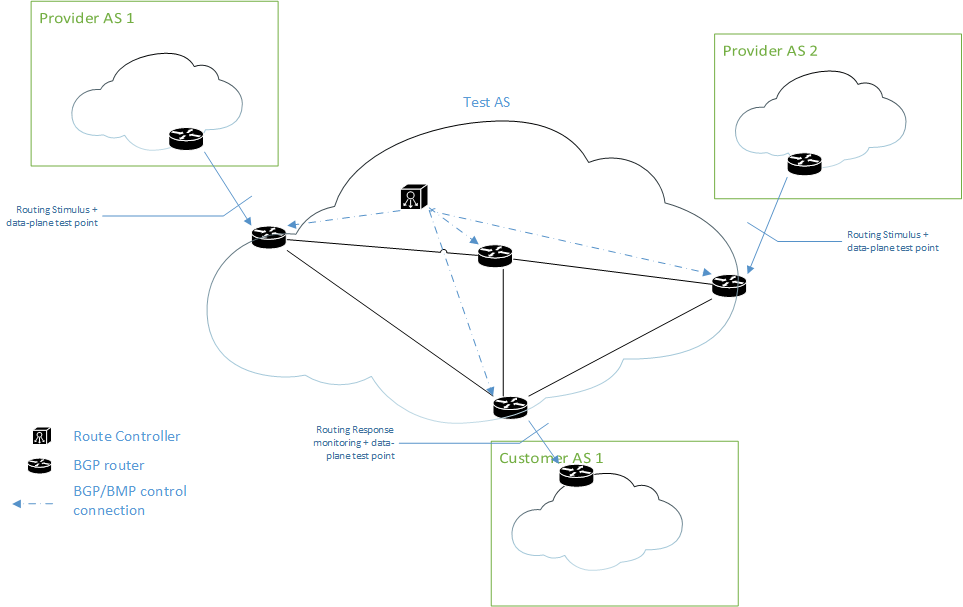
\includegraphics[width=0.5\linewidth]{images/simulated test network 1.1.png}
	\caption{Figure 1- Proposed Architecture}
	\label{fig:enter-label}
\end{figure}
% Figure 1- Proposed Architecture

\subsubsection{Route Controller Policy Agent}

The proposed Route Controller is presented above as a ‘black box’, which takes as input routing state information and produces as output routing decisions. However, the Route Controller only has value when the routing decisions it makes are better than those made by the existing classical routers. The topic of Routing Policy is too broad for any single work to address effectively; the intention in this thesis is to develop an instance of a Policy Agent for the Route Controller which exemplifies some of the possible attributes which the architecture enables. Some example important capabilities which will be explored in this work are:

\begin{itemize}
	\item Use of historical context to inform routing decisions
	\item Use of topological analysis to inform routing decisions
	\item Use of formal policy descriptions to inform routing decisions
\end{itemize}

%%% {\color{red} from document file: PIR / Thesis use cases}

\section{PIR / Thesis use cases}

\section{IDR applications}

It can be expected that the enabling impact of a programmable network will drive many more applications of immediate practical value as network operators awareness grows, but there are already plenty of examples which underline the value of the proposition in Internet routing applications, of which few are listed here:

\begin{itemize}
	\item enhanced re-routing based on fault location signalling
	\item route quality assessment before selection
	\item BGPSEC with acceptable performance
	\item Artemis style prefix hijack prevention
	\item route leak detection and mitigation (current PIR use case)
	\item route selection based on route stability (‘smart route-flap prevention’)
	\item smart load-balancing
	\item peer-specific preemptive route monitoring (‘active mode monitoring’)
	\item application of ML to routing
	\item use for AS internal security and diagnostic operations - e.g. traffic scrubbing, traffic monitoring, by injecting application specific route using flowSPEC
\end{itemize}
Similar challenges to traditional transit routing exist at IXP route-servers, and PIR offers the prospect of customised curated route selection based on diverse criteria. Indeed, many of the benefits of PIR are most applicable to routes exchanged at IXPs, and PIR also offers the prospect of mitigating some of the disadvantages of route servers as perceived by ISP members at IXPs.

Two of these applications are described now in a little more detail to demonstrate the immediate wider applicability of a PIR approach to IDR.

\subsection{enhanced re-routing based on fault location signalling}

A well known problem in BGP networks is the phenomenon described as ‘path hunting’ or path exploration, or ghost ....? See ....?. Path hunting is a process which takes place after a route failure and typically delays the process of converging on a new operable end-to-end route. In essence, path hunting is caused by short lived advertisements of unviable routes which also pass through the point of failure which triggered the first routing update. These transient unviable routes are generated by stale routes by routers situated close to the failure location.

There have been previous proposed solutions to this problem which either modify BGP protocol to signal fault location, or to propose systems which can infer route failure locations and make alternate route selections to those which are received as a result of path hunting. Whilst PIR could be put to use to implement those earlier proposals, this new design builds on that work whilst offering a more practical and readily deployable incremental approach to the same problem.

\subsubsection*{Methodology}

%%% <// this is more problem description than solution..

BGP routers are unaware of network topology, other than the restricted set of AS systems which are identified in routes received for routers closer to the route origin. After a link failure occurs in the currently announced path the eventually discovered working alternate path will likely differ significantly from the failed path at some location close to the origin, although that viable alternate may have to propagate though many of the same AS systems as those which lay on the failed path, and thus appear similar to both the original failed route, and also the subsequently propagated transient but unviable routes. Unfortunately however, the unviable routing messages which are received cannot easily be distinguished from the eventual first arriving good route. A further complication may arise in that there may be a complementary ‘storm’ of good routes as the new working routes are propagated at different rates through the intervening networks. An ancillary effect is a multiplication of the number of changing data points by the numbers of individual prefixes which were originally routed through the point of failure, some of which prefixes may eventually convergent to distinct routes after reconvergence and stabilisation is complete. But in this storm of routing information one piece of information is entirely missing, and not easily inferred, which is the actual point of failure, and even the fact that there \textit{is a} point of failure: route changes may as likely arise from added links as failed ones (the numbers of such events should of course balance out!). The reason for this dearth of information on failure locus is that the BGP failure message - ‘Withdraw’ - is most often replaced by a new route, and so either never propagated or only widely propagated very late in the path discovery process. Indeed, it is probable that if withdraw is received at all, for many routers it is the very last routing message to be received before a new viable alternate is received. The late arrival of withdraw is one reason that failure location signalling is hard to implement with much utility: the second is that the Withdraw message itself carries no information at all, other than the prefixes which can no longer be routed. So, when Withdraw is seen it is not possible to know where it originated, or even if its cause is a link failure, as opposed to a policy or configuration change.

%%% //>

\subsubsection{Variations on RCN}

Basic path exploration presents as updates to existing routes which are simple AS path extensions in which additional AS numbers are inserted in the previously received path. The failing AS is identifiable as the last unchanged AS in the path. At the failure locus the ghost routes are received from distinct peers, whilst at downstream points the replacement path announcements are combined within an announcement stream from a single peer, and mitigation options are different in the two cases. RCN proposed that, in the first case, withdrawal should be sent, before sending any further announcements.

It is worth analysing the objectives of RCN: ultimately, the goal is to rapidly restore service, however a subsidiary objective, which may also indirectly contribute to faster restoration, is to reduce transmission of ‘ghost routes’. In default BGP Service restoral depends on ‘bad’ routes being flushed out: ghost routes may directly delay this if they are still somehow preferred over the eventually selected stable alternate. Ghost routes can also delay restoral indirectly in two ways:

\subsection{route quality assessment before selection - ‘route curation’}

\subsubsection{Context}

For each routable prefix or group of prefixes an AS may receive routes from many sources: and in order to provide best service the AS selects just one route, but, lacking any stateful logic, the selection process is entirely reactive and depends only upon the instantaneous routing state. There is some justification for this approach: it is simple and predictable, and enables very rapid, locally decided, re-routing under topology change. However, the approach is hardly optimal: and almost every kind of routing failure or sub-optimality can be argued to result from this strategy. In a sense, that observation is trivial: if an outcome of a system is suboptimal, then the system can be improved.
But, the point is that making more refined decisions requires more complex logic, which may require a different processing approach. In essence, this is the heart of the PIR proposition.

This proposal is about an alternative operational strategy which aims to combine the advantages of simple distributed stateless route selection with the benefits of a more complex analytical approach. The approach is based on some simple reasonable assumptions about both network failure context, and about network routing threats. Concerning failures:

\begin{itemize}
	\item That rapid routing decisions are only required when responding to events which cause service failures.
	\item In many cases where an immediate response is required, the optimal alternate route selection is already available since long before the triggering event
\end{itemize}
Concerning routing threats

\begin{itemize}
	\item Adverse routing announcements are generally received and selected as ‘improvements’ over existing adequate routes.
	\item A potentially problematic exception to the first assumption is the case in which a preferred route source has already unwisely accepted an adverse route. However, even in this case a good, well established second-best candidate may be available.
	\item When the first assumption fails completely, i.e. no good alternate route is known at the local AS, then there is no sufficient AS response which can mitigate the problem
\end{itemize}
If these assumptions hold then a simple AS level behaviour exists which can improve network service by protecting against failures with rapid responses whilst applying more intensive analysis to new routes and thus enabling adverse routes to be rejected.

The AS behaviour required is this:

\textbf{Definition of Curated Route} For every received route an arbitrarily intensive analysis can be executed, and an aggregate preference calculated - this is similar to local preference, and it is likely that local preference attribute could be used to implement the strategy in a classical BGP network. Once a route has been analysed and scored it is made available for unrestricted selection - such routes are called ‘curated’ routes. As updates to existing routes are received from peers the curated attribute may be revised: depending on many factors the new route might be temporarily accepted into the curated list, possibly with a lower initial preference, or excluded until fully validated. The entire set of curated routes corresponds to an extended, AS wide, ADJ-RIB-OUT, such as might be implemented for ADDPATH.

\textbf{Application of Curated Routes}

At an AS level the principle is simple: whenever a curated route is available for a prefix it should be selected and announced: potentially, different curated routes could be announced to different peers, for business/policy/traffic engineering reasons. In one interpretation all curated routes should be immediately usable, e.g. a full operational MPLS path to the prefix via the originating external peer is available from any ingress ASBR. This interpretation would allow granular unrestricted selection between diverse routes within the AS.

\textbf{Curated Routes Impact on Route Selection}

The curation principle is simple: for all route selection, curated routes are selected in preference to non-curated ones, based on relative preference in all cases.

In practice this may be as simple as defining all directly received routes to have a local preference greater than some minimum, so that all curated routes are preferred. A refinement for this principle would be to allow specific border routers to assign ‘curated’ level preference to specific selected directly received external peer routes. The operational objective is defined at the AS level is simple, but the implementation detail in a classical AS is subject to design - not all curated routes are necessarily distributed to every border router, and various methods of distribution can be considered. an important aspect of a concrete implementation architecture is the decision about which curated routes to distribute, and to which border routers.

\section{Other BGP applications}

\subsection{Data centre}

BGP is already widely used in data-centre contexts, both multi-tenant (‘cloud’) and single tenant/enterprise. PIR techniques can easily be applied here too, for example for management of internal route selection security policy, or implementation of application specific route optimisation. BGP flowspec can easily be used to provision application specific routes in the dataplane, but the risk of complex and frequently updated router configurations are a disincentive to such innovation. Using an overlay controller based on PIR would enable such innovation in a controlled and fail-safe way. PIR could be used in conjunction with automatic configuration management systems to evaluate routing optimisation designs.

Application specific traffic routing is already widely used in enterprise settings, but in most cases the implementation requires customised hardware (middle-boxes). A programmable BGP controller using BGP and especially BGP flowspec could replace many such complex systems and unify the routing design into a simpler, more flexible, SDN style network fabric.

PIR could also find application in multi-tenant BGP environments, where it could be used in conjunction with

\subsection{Ethernet VPN (EVPN)}

EVPN is rapidly emerging as a useful technology for large scale (non-internet) service provider networks, e.g. Sky Broadband deployment in Italy (cite UKNOF London 2019).

Without a controller capability it is as difficult to manage EVPN systems as it is the global internet, i.e. the distributed static policy configuration approach does not allow complex or granular policies to be applied. PIR is a natural candidate for enhancing the manageability of such networks.

    \chapter{Implementation}
 {\color{red} the following is from the rejected paper on performance measurements (kakapo)

  It is a place holder for more text which is not ready yet....
 }
\section{BGP performance characterisation}

% % \label{sec:motivation}

\begin{figure}[h!]
	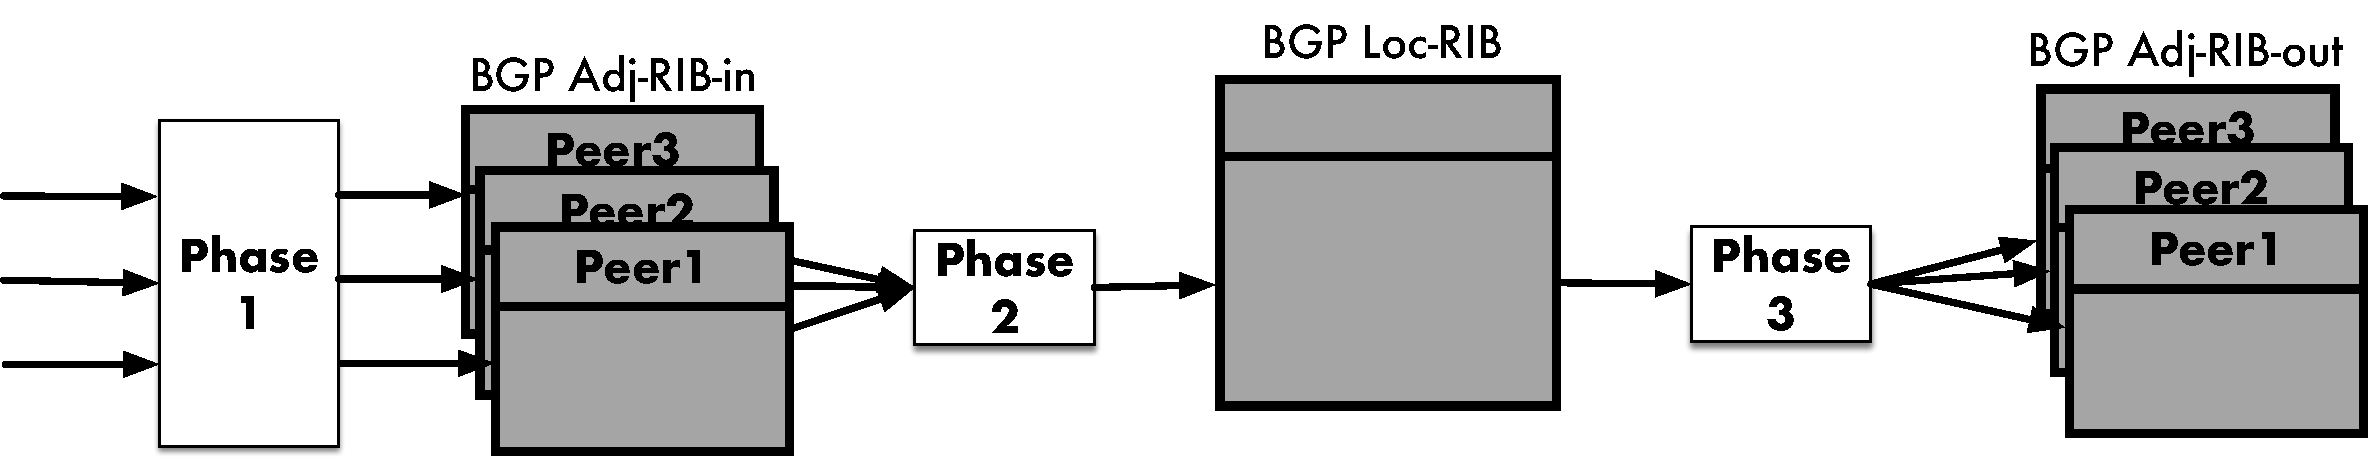
\includegraphics[width=\linewidth]{images/routeSelection.pdf}
	\caption{The BGP protocol defines a complex processing pipeline for route updates, which relies on multiple data structures to maintain intermediate information.} \label{fig:routeSelection}
\end{figure}

In this section, we briefly discuss the performance bottlenecks of a BGP speaker
and motivate the design of our system with a set of recent use-cases.
Processing route updates is the core functionality of a BGP speaker. The
processing algorithm consists of three phases, depicted in
Figure \ref{fig:routeSelection}, and precisely defined in the BGP protocol
specifications~\cite{rfc4271}. {\it Phase 1} processes, filters and rank
routes, based on the local speaker configuration. Filtered routes from each
peer are stored in the Adj-RIB-in tables, alongside intermediate processing
results and also linkage information between input route updates and main RIB
entries.  {\it Phase 2} compares all available routes for each prefix, using
Phase 1 ranking outcomes and elects a single route for each prefix.  This stage
stores its route selection results in the global BGP Loc-RIB table.  Finally,
{\it Phase 3} filters and modifies the selected routes from Phase 2 based on
peer-specific policy, potentially modifying path attributes such as
communities, AS path, MED and LocPref.
Stage 3 results are stored in per-peer Adj-RIB-out tables.

BGP speakers must maintain and manage a highly complex routing state which
expand to multiple GB of main memory in a core router. As a result, reasoning
about their performance is difficult and depends heavier on the BGP trace
characteristics. Network operators frequently revert to major investment in
specialized hardware in order to recreate realistically network conditions and
explore the impact of different tuning parameters on the speaker performance.
In parallel, the use of specialized hardware leads to limited widely acceptable
measurement standards. In order to further highlight the measurement challenges
we discuss two specific BGP use cases.

\textbf{IXP and Route Server scalability:} The increasing importance of Internet Exchange Points (IXPs) and Route Servers
(RS) leads to new scalability challenges for software BGP speakers.
RSs must support an unprecedented BGP workload including significantly larger
RIB sizes and peer numbers, as well as providing multiple independent `views'
or RIBs, each enforcing unique policies. Although IXPs employ existing open
source speakers to implement their RSs, the majority of these projects remains
single-threaded and lack the ability to easily ``scale-up'' during
high-utilization periods. Such limitation drove Google to implement Raven,
a proprietary multi-thread BGP speaker for their SDN-enabled edge peering
infrastructure~\cite{Yap2017}. Network operators require a standardized
methodology to evaluate the performance of BGP speakers under extreme load
conditions.

% Can we move these into the result section?

% The current favoured solution for this role is Bird, based on its
% rich and flexible policy configuration language and its superior performance.
% However Bird and its direct competitors FRR and OpenBGPD remain effectively
% single threaded systems \footnote{OpenBGPD implements a single separate thread
%     to manage the Route Decision Engine, however our tests indicate that this
%     provides a very small contribution to performance under stress since the
%     other threads utilisation remain low whilst the RDE engine is working at
% 100\% CPU} unable to benefit from multi-core systems: this limitation drove
% Google to implement a proprietary new highly parallel BGP speaker {\it Raven}
% for Espresso\cite{Yap2017}, Google’s SDN-based Internet peering edge routing
% infrastructure.  In this context the need to quantify the limits of performance
% and scale for Route Servers thus takes on a higher level of significance.

\textbf{Next-generation BGP speaker architecture:} A number of studies have
identified challenges in the design of BGP speakers and have proposed novel
architectures to improve their performance and flexibility. For example,
Keller \textit{et al.}\cite{Keller2010b} have proposed a virtualization architecture for
BGP speakers, that allows easy state migration,
while Grover \textit{et al.}\cite{grover2011} have developed a multi-threaded routing protocol
platform and evaluate the impact of different task scheduling approaches.
Unfortunately, the lack of a generic open-source performance evaluation does
not allow a comparison in the impact of the proposed changes in BGP protocol
processing performance.
\section{Architecture}\label{sec:arch}

Characterising BGP speaker performance entails several major challenges.
Firstly, whilst traffic generation should conform to basic BGP protocol
semantics in order to ensure interoperability, modified BGP software routers to
generate realistic traffic can incur processing overheads, limit traffic
generation capabilities and potentially introduce measurement artefacts.
Secondly, to study BGP speaker behaviour in resource poor environments requires
fine grained resource control, in order to emulate the CPU and memory
constrained processing environment available in actual network devices.
Thirdly, the measurement task still requires reasonable standards support
to accommodate a wide range of experimental scenarios.

To address these challenges we develop an holistic BGP characterisation
framework. The platform consists of two main components: {\it kakapo},
a flexible and high-precision BGP testing framework, and
	{\it Kagu}, an experiment automation tool offering precise resource control
and monitoring capabilities, using CPU virtualization technologies.  An
important supplementary component of {\it kakapo} is a lightweight BGP
relay/proxy, {\it kakapo-relay}, which allows us to characterise the baseline
performance of kakapo as a monitor and load generator.  Performance
measurements obtained from kakapo with kakapo-relay as the System Under Test
provide confidence that observed performance envelopes for BGP speakers are not
artefacts of the measurement infrastructure.  For the rest of this section we
discuss in detail the design and functionality of each component.

%\begin{minipage}[c]{.45\linewidth}
\begin{figure}
	\centering
	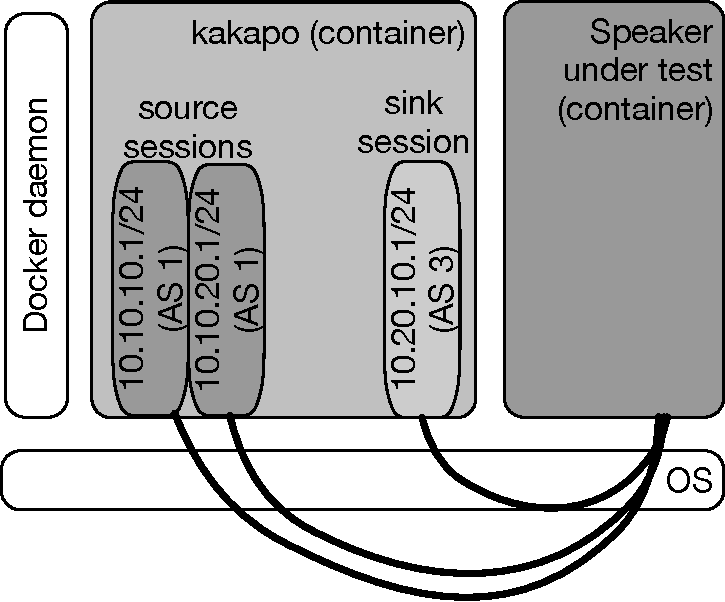
\includegraphics[width=.45\linewidth]{images/arch.pdf}
	\caption{Kakapo architecture.}\label{fig:arch}
\end{figure}

% \begin{minipage}[c]{.45\linewidth}
%     \centering
%     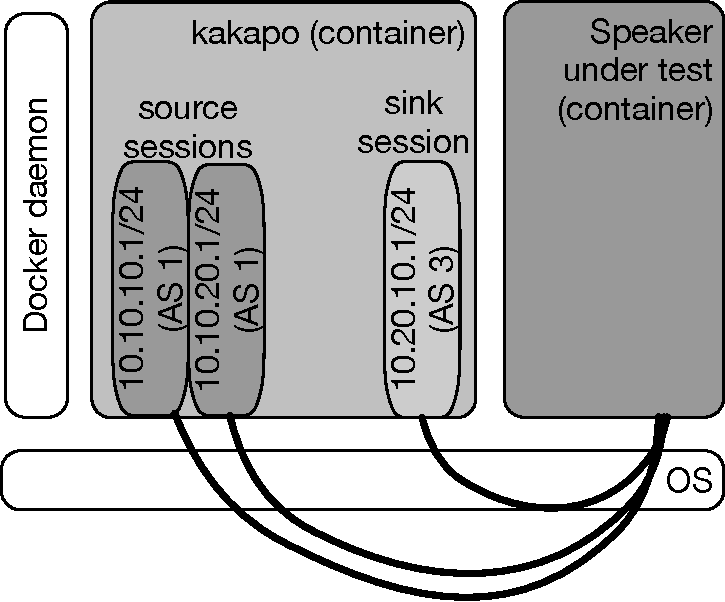
\includegraphics[width=\linewidth]{images/arch.pdf}
%     \captionof{figure}{Sample
%     sequence diagram for a bursty single-peer kakapo
% experiment.\label{fig:traffic-model}}
% \end{minipage}
% \begin{figure}
%     \centering
%     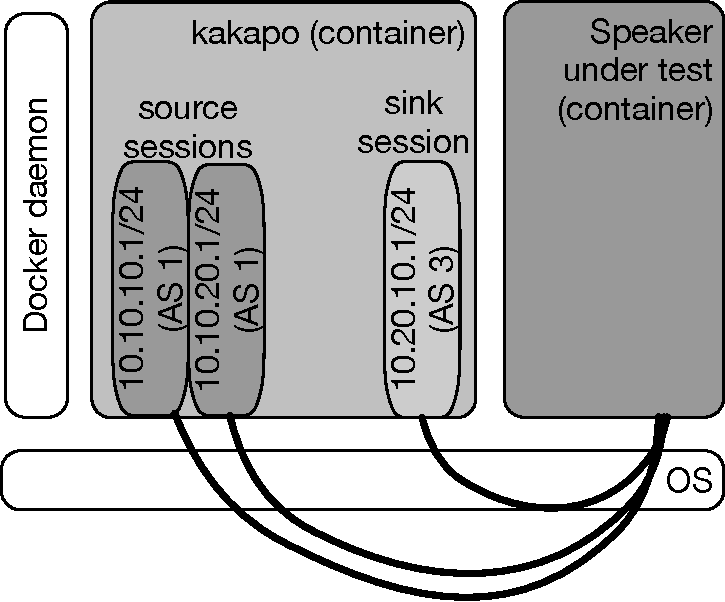
\includegraphics[width=0.5\linewidth]{images/arch.pdf}
%     \caption{Enter Caption}
%     \label{fig:enter-label}
% \end{figure}
\subsection{Kakapo: BGP performance characterisation}

% High level overview of the system
Kakapo is a high-precision BGP traffic generation and monitoring application
written in C. It is designed to measure the performance of a BGP speaker for
varying load conditions by measuring the time to process a number of BGP
messages. Kakapo uses a black-box testing approaches and relies solely on BGP
message times to understand the impact of the protocol load on the speaker
performance.  In order to perform the measurement, kakapo establishes multiple
parallel BGP sessions with a speaker and emulates the behaviour of multiple BGP
speakers. Kakapo BGP sessions are RFC-compliant, relying on a minimal complete
BGP Finite State Machine, thus allowing the test system to measure the
performance of any software and hardware router.

% Describe how things are connected
The architecture of kakapo is depicted in Figure~\ref{fig:arch}. For each
experiment kakapo establishes a single passive sink (monitor \& measurement)
session towards the speaker, and one or more source (traffic generation)
sessions, with each session configurable in terms of BGPID, AS number and
Optional Capabilities.  Each experiment commences by initialising the BGP
speaker under test (BSUT) with an empty RIB and configured to ensure that
routes received from the emulated source test peers will be imported into the
RIB and re-exported towards the destination sink test peer.  Typically, the
BSUT and sink peers are configured in the same AS (iBGP sessions) whilst the
sink peer is in a different AS, (eBGP session).  If the BSUT has a configurable
MRAI (Minimum Readvertisement Interval) timer this must be disabled to ensure
that route updates are always promptly re-announced.  As a result, every route
advertisement or withdrawal from a source session causes the speaker to
immediately transmit a corresponding route update to the sink session, once the
route has been processed.  By orchestrating both the sinks and the source
stream from a single application the system can precisely measure timestamps
and thus RTTs for each update.

% In operation kakapo implements concurrent multiple BGP speaker
% endpoints, using distinct network addresses at the same host, usually
% configured as loopbacks.

% Describe how data are generated
Kakapo allows experimenters to execute a wide range of measurement scenarios.
Firstly, the application allows an experiment to target both initial RIB population and RIB update performance, by controlling whether BGP sessions are reset between experimental runs.
Secondly, route traffic generation can either be bursty, where updates are transmitted in batches, or continuous, where route updates are transmitted continuously using a closed-loop mechanism that ensures a fixed number of updates is always in-flight.
Finally, experiments can control the number of source BGP sessions, and if more than one source are configured, to control which sessions generate route updates.

% measurement details
The principle type of measurement is the elapsed times between bursts of updates
sent by the source until the corresponding updates are all received at the
sink.  Updates are typically sent in discreet bursts, and the time taken to
send and receive these bursts is also measured, in addition to the delay
between sending and receiving.
% The BSUT is expected to be
% configured such that it imports some or all routes from the source and exports
% some or all routes to the sink.

Kakapo experiments have a three-phase lifecycle:
conditioning, main mode and termination.  During conditioning,
full route tables (Adj-RIB-In) are established for all route source
peers. During the main phase, further updates are generated however all subsequent
Updates are for prefixes which have already been announced by all peers.
As a result, the size of all RIBs is fixed, allowing
experimenters to evaluate the effect of different size route tables.
During the termination phase, all peer sessions are terminated by sending BGP
Notifications.  This phase offers the opportunity to evaluate the propagation
latency of these route withdrawal through the BSUT. Unfortunately, practical
experience developing this tool has revealed several inconsistent
BSUT behaviours and the lack of a simple mechanism to identify the `last'
withdrawal, does not allow to isolate their effects.

Continuous mode measurements are implemented by transmitting an
initial burst sequence of updates: the traffic sink accepts the resulting
Update stream and responds by transmitting additional further updates on the
source session(s) in order to maintain the in-flight quota at the
pre-configured level.  The principal objective of this test is to characterise
the continuous performance capability of the BSUT.  This requires that the
transmit `credit' window is set sufficiently large.  We observed that a value
of around 5,000 Updates was sufficient to drive all of the systems in our study
to their maximum rate, without incurring unnecessary congestion and buffering
latencies.

The traffic generation model must ensure that initial route announcement
precisely populate a set route table size, while subsequent routes announcement
are always selected by the BSUT, in order to be announced to the sink session.
In order to ensure this requirement we exploit the Local Preference attribute value.
Since Local Preference is a 32 bit value there is a possibility of wraparound
if every Update incremented LocPref, hence we only increment LocPref value when
wrapping around the complete RIB.  Thus during the initial conditioning phase
the most recent transmitting peer is always the source of preferred routes, and
the full route table is re-announced by the BSUT for each connected source
peer.

Kakapo synthesises route prefixes sequentially, using a configurable initial
seed IP address and a configurable prefix length.  Kakapo also enforces
continuous changes in AS path content (but not length), firstly because sending
duplicate routes is not permitted, and also for diagnostic purposes and to
allow future extension to individual message correlation.  Paths are also
customised based on source peer.  Customisation is based on modifying
intermediate AS numbers in the AS path.

Real world internet route tables have varying numbers of prefixes in each
update: a complete table contains typically around 750k
prefixes\footnote{{http://www.routeviews.org/peers/peering-status-by-as.html}}
and 150k distinct routes, which is an average of about 5 prefixes per unique
Path.  Kakapo produces uniform Routes with a fixed number of prefixes per Path
- in almost all of our experiments reported in this paper we use a 160k/5
profile - i.e. the full table is size is 800k with 160k distinct origin ASes.

	{\it Canary routes} is a technique used to determine when route processing has
been completed in the cases where some or all transmitted Updates are {\it not}
re-announced, and also simply for confidence that an experimental phase has
fully completed.
%This experimental mode enables measurement of an important and different distinct performance attribute to the case where all received routes are re-exported.
Since in real world operation it is often the case that received routes will
not be preferred and re-announced, it is difficult to measure this
outcome precisely due to the lack of a notice for the processing completion.
Canary routes are simply routes which are
constructed such that they will always be propagated: typically this means that
for each source peer a different unique canary prefix is defined.  By sending
a canary Update after a test burst which is not expected to be propagated we
can measure the processing delay by simply timing the delay before the canary
re-emerges.  This strategy relies on the BSUT processing routes in strict
sequence for a given peer, which must be independently confirmed for each BGP
speaker.  All of the BGP speakers in our study did exhibit this behaviour,
including those which claim or exhibit multi-threaded processing capability.
Canary routes also provide a good method for troubleshooting invalid
configurations - since kakapo currently does {\it not} correlate every
transmitted and received messages it uses simple counts of messages to
determine when a burst has been completely received.  By transmitting a canary
as the last message in a burst, kakapo can quickly detect and report when some
Updates have been dropped.

In order to evaluate the base performance of our measurement platform, the
kakapo codebase contains the kakapo-relay application, a reference BGP speaker
supporting the minimal functionality required to peer with the kakapo system.
The purpose of kakapo-relay is to provide a benchmark measure of the
performance capability of the test harness and characterise any measurement
artefact incurred by the platform. Kakapo-relay is written in C and uses iovec
and epoll to achieve low latency and line rate network throughput in realistic
BGP test scenarios.  Both kakapo and kakapo-relay optimise network performance
by working with very large buffers and executing read and write operations
which typically address very large numbers of BGP messages in a single system
call.  The continuous rate measurement design is especially sensitive to
efficiency issues: if kakapo transmits updates too quickly, it forces much
smaller messages at network Layers 2 and 3, which pushes up the CPU demand for
the target systems and results in much lower performance than would be the case
if Updates are transmitted in slightly larger blocks.  Since our objective is
to establish how fast the BSUT can perform under optimal conditions we adjust
the transmit block size parameter to ensure that TCP and Ethernet transfers are
large enough to avoid this effect (but still much smaller than the `in-flight
window').  However it should not be ignored that in many real world scenarios
routing traffic packet scheduling may not be so optimal, and thus these BGP
speakers may perform even less well than our measurements show.
% Whether
% distributing load over multiple physical interfaces would improve matters is
% a matter for further investigation.

\subsection{Kagu: BGP experiment automation}

A major challenge for network experimentation is reproducibility. Kagu is an
automation platform, built around kakapo, allowing experimenters to deploy and
parallelize the execution of BGP experiments. In parallel, kagu also automates
measurement data and logging information collection for offline processing.

OS virtualization is a key technological enabler for Kagu, which supports
integration with docker and the libvirt management library.  The docker
integration allows kagu to run kakapo and software router as docker containers
and to use docker management operations to spawn and terminate them.
Furthermore, detailed logging information are collected through the
systemd/journald services in the container. In order to run an experiment, the
platform requires as input the router and the kakapo configuration parameters
and the platform will use docker technologies to execute the experiment and
collect the results.

Furthermore, libvirt integration allows kagu to deploy large-scale experiments
with complex network topologies over a hypervisor-based virtualization
platform, like KVM. VMs derive from a base Ubuntu image with the dockerd
daemon installed and configured to exposes remote access via HTTP.

During the deployment of a multi-host experiment, kagu builds all the required
virtual links between VMs, as well as a control plane network which uses
dynamic DNS and cloud-init to map VM control interface addresses to user
friendly host names. A custom libvirt network topology provisions distinct
unique virtual network address blocks onto each VM and dynamically updates the
configuration of a local DNS server.  Finally, the framework offers an
arp-router agent which install routes to loopback and allows connectivity over
unnumbered network interfaces.

Both test harness (kakapo) and target systems are bundled as Docker images
which enables them to be easily started and stopped in remote virtual machines
using the ‘remote Docker’ feature.  Remote Docker allows standard Docker
commands, such as ‘docker run’, ‘docker kill’ and ‘docker pull’ to be executed
on arbitrary target systems from a single controlling machine  Thus a cluster
of multiple VMs having varying resource capability can easily be orchestrated
to run multiple sets of experiments in parallel.  A complementary set of
scripts (kakapo-virt) is used to create and provision the target virtual
machines.

The main system elements are:

\begin{itemize}
	\item kakapo core  a ‘C’ language BGP test tool which can act
	      as a BGP peer, operating simultaneously in both route sink and route source
	      modes
	\item kakapo relay  a ‘dummy’,‘C’ language, BGP router which allows
	      baseline calibration of the test system
	\item kakapo runner  a run-time
	      integration framework for controlling multiple test runs with ranges of
	      test parameters
	\item kakapo ingest  offline analysis of the test data
	      generated by kakapo, including on-demand gnuplot graph display
	\item
	      kakapo-virt  a VM and virtual network provisioning tool --- kakapo virt
	      creates and provisions test VMs with different resources (CPUs, RAM,..) to
	      provide execution environments for kakapo targets and test harness instance
	      to execute in.  Kakapo-virt also provisions both a control plane network to
	      allow remote orchestration of the VMs and their Docker execution
	      environment, and a separate experimental network context which meshed VMs
	      which are configured to operate as a single experimental topology
	      somewhat like mininet, but for KVM virtual machines.

	\item kagu a build and deploy system for the (mostly Dockerised) components of kakapo
	\item arproute a network utility which enables virtualised systems to discover routes between themselves without manual configuration.
	\item Docker, systemd, libvirt and nginx with webdav support --- provides the infrastructure environment in which kagu and kakapo operate
\end{itemize}

Of these components some work before a testing session (kagu, kakapo-virt), and
others after testing sessions have finished (kakapo ingest).  The core system
consists of kakapo core, kakapo relay, kakapo runner: of these kakapo runner
is the coordination tool: it schedules execution of test systems in virtual
environments, typically systems consisting of kakapo core paired with another
BGP speaker such as bird, frr (quagga), OpenBGP, hbgp, or another hardware or
software router.  Kakapo core starts and stops BGP peer sessions with the
SystemUnderTest, monitors the response performance and records the
configuration and results in test data files on a centralised storage system
for later analysis.  Kakapo runner feeds the required test parameters to kakapo
core: typically these specify a range of BGP route table sizes (two
parameters), and a cycle count for the number of repetitions of route changes
to send, updating the initial route table load.  The recorded results are delta
time measurements for the begin and end of both reception and transmission of
groups of Update messages.  Results are uploaded as structured text files to
a webdav server.

% % \subsubsection{Docker usage}

% % \subsubsection{kakapo-core}

% % \subsubsection{kakapo-relay}

% % \subsubsection{Linux TCP / kernel limitations}

% % Observations of the network behaviour of both the existing platforms such as
% % frr, bird and OpenBGP, and also the custom implementations developed for the
% % study (hbgp, kakapo and kakapo-relay) show the impact of Linux TCP
% % implementations and default configuration

% \subsubsection{Data analysis --- kakapo-ingest}

% Kakapo-ingest is an offline tool which consumes the output generated by
% kakapo-core.  Kakapo currently uses webdav as a repository access mechanism: at
% the end of every execution of a single kakapo run a text based data file is
% uploaded to a central server using webdav.  The file format captures ‘metadata’
% such as the kakapo parameters defining RIB size, update blocking factors,
% prefixes per update, as well as all significant context for the experiment,
% e..g the software router name and version, the number of cores and RAM
% allocation, the date and time of the experiment, and the ‘topic’ which is used
% to group a group of experiments which collectively define an entire
% ‘experiment’

% Kakapo-ingest is a tool whose purpose is to select and preprocess the raw data
% from multiple kakapo-core runs into a format suitable for graph plotting or
% further analysis.  K-ingest resembles an SQL query tool in that it requires
% a set of selection terms to be given which represent a filter over the total
% set of data points.  The Query syntax allows an explicit selection of
% a ‘x-axis’ variable and a separate discrete multi-line selector value set,
% combined with filter terms which define specific values which must match data
% points in order to include them.

% In operation Kakapo-ingest takes a directory path (/var/webdav in the example
% below), and recursively scans it for data files in the correct kakapo format.
% Kakapo-ingest has several modes of execution which allows the dataset to be
% queried and selection criteria defined up to the point that a coherent set of
% data points can be extracted and plotted in a gnuplot graphing environment.

% An example k-ingest query is:

% ingest /var/webdav TOPIC=RIBTEST PLATFORM=bird,frr,bgpd,hbgp RIBSIZE=?

% % In this example, a graph is defined using the metadata field ‘RIBSIZE’ as the
% control parameter (y-axis), and showing separate plots for each of the named
% platforms (bird, frr, OpenBGP, haskell BGP).  In this case there were no
% variants such as CPU count or RAM size present in the database, and so the
% query is already unambiguous and able to directly generate a gnuplot data file
% and if required plot it interactively or export to a graphic file.  Otherwise
% additional selection terms would be required, such as

% ingest \ldots CORES=4 MEMORY=8192

% The flexible query syntax enables other parameters to be plotted, for example
% a graph showing performance for different numbers of prefixes in a fixed count
% of Updates is possible simply by changing the control parameter to ‘GROUPSIZE’
% and defining a suitable range of parameters in kakapo-runner to create the
% required dataset.

\section{Characterising BGP speaker performance}\label{sec:result}

To demonstrate the capabilities of the kakapo and kagu systems we conduct
a performance analysis of a representative set of production software BGP speakers.
Specifically, using a virtualised server testbed (\S~\ref{sec:testbed}), we evaluate the
single and multi-session performance.

\subsection{Measurement setup}\label{sec:testbed}

Presently, network managers have access to a wide-range open-source BGP projects
with carrier-grade protocol support. FRR~\cite{frr} is a multi-protocol routing suite
with support for BGP. The codebase is an active fork of the Quagga project and
this speaker software is widely deployed in IXP infrastructures, as a route
server . Additionally, the code is used by white-box
vendors to provide routing protocol capability for BGP and other protocols in the control plane of their network devices.
BIRD~\cite{bird} is another widely used BGP speaker, considered to offer consistent performance,
and a rich configuration paradigm. BIRD has recently undergone a major
rewrite to integrate simultaneous IPv4 and IPv6 support, thus in our analysis we include both
version 1.6 and 2. In our analysis we also include OpenBGPD~\cite{openbgpd},
an minimal open-source BGP speaker maintained by
the BSD community, offering an alternative stable and secure BGP protocol support. Finally,
in our analysis we include GoBGP~\cite{gobgp}, a multi-threaded BGP speaker written in Go.
GoBGP proposes to capitalize on the parallelization capabilities of the GO language to provide high-performance BGP
support. However, the choice of a high-level language, in comparison to
other BGP implementation written in C, exhibits interesting challenges for overall
system performance. In our measurement study we employ FRR (v7.0), BIRD
(v1.6.6), BIRD2 (v2.0.4), OpenBGPD (v6.5) and GoBGP (v2.6.0).  All BGP speakers are
configured so as {\it not} to export routes to the local FIB.

Using kakapo we develop four representative tests. Firstly, we measure the
latency to perform a {\tt table transfer} of 800k routes. Table transfer are
a common event in the global Internet, which can significantly increase the
load of a BGP speaker and increase latency~\cite{Cheng2011}. Secondly, we measure
the latency to process a burst of 50k {\tt route updates}. Large burst of route
updates is a common effect during route instability incident. Finally, we
develop a simple rate estimation measurement to evaluate the multi-session
scalability of speakers. Specifically, kakapo develops a close loop traffic
generation mechanism, that synchronises route transmissions from a source with
route advertisement on the sink session and target to maintain a constant number
of route update in-flight at any point in time. By conducting an exhaustive
analysis of many possible window sizes for this measurements, we concluded in
using a window size of 5k routes for all platform measurements. This window
size creates a significant load on the BGP speaker, but does not result in
congestion. Using the aforementioned measurement scenario, we measure in
a multi-session setup both the average {\tt single-session burst rate} (a
single session generates the update stream) and {\tt multi-session burst rate}
(all sessions generate in parallel updates), when transmitting a continuous
update stream for a statistically significant amount of time (30 seconds).

All our tests are executed on a Dell server, equipped with two E5-2690 Intel Xeon
CPUs (2x24 Cores) with 320GB of RAM and an Intel X540-AT2 10~GbE Copper
card. All experiments are executed using docker containers. To ensure
representative high routing link performance we configure kakapo and the BGP speaker to transmit their
updates over a loopback link between two ports of a 10G NIC.

% \subsection{Single-session performance} \label{sec:single-peer}

% \input{single-host-tbl}

In order to establish a set of baseline measurement profiles, in this section
we focus our performance analysis on the single session scenario using the
metrics discussed in the previous section.  Our measurement results are
presented in Table \NH{XXX?}, reporting the mean and the standard
deviation of each measurements across 50 runs. In order to demonstrate the low
measurement overhead of our platform, the table reports additionally the
performance measurements of our custom BGP relay implementation. The relay BGP
speaker completes the table transfer in less than 90msec, while the processing
of the route updates complete in approx. 30 msec. This measurements suggest
that the impact of our measurement in the overall latency measurement is less
than 10\%. In parallel, our system generates 4x more updates than the BIRD2
speaker can process, the fastest BGP speaker in this measurement.

Furthermore, our measurement highlight that there is a significant latency
difference between a table transfer and a route update for most speakers. This
can be attributed to the significant number of memory allocations that the
speaker needs to perform in order to create the required state for each new route.

In terms of performance, we highlight that BIRD2 achieves the best performance
across all metrics. In addition, BIRD2 exhibits a non-negligible performance
improvement in comparison to BIRD. Specifically, BIRD2 processes 100 msec
faster on average the table transfer and the route update and its average
processing rate is improved by 15\%. FRR is significantly slower than BIRD and
BIRD2, especially for the average processing, which is 4x time slower in
comparison to BIRD2. Nonetheless, from a network manager perspective, FRR
supports series of configuration options, not available in BIRD. OpenBGPD
performance is measured to be somewhere between the two systems. Finally, GoBGP
exhibits the worst performance in comparison to the rest of the BGP speakers.
During our measurements we note that the GoBGP process was saturating 6 CPU
cores, which suggests that the speaker was using effectively its multi-thread
capabilities. The measurement results suggest that the use of a high-level
language (Go) can have an impact on the performance of a BGP speaker, due to
features like automated garbage collection,
while enabling multi-thread support in a BGP speaker is not guaranteed to
improve overall performance.

\subsection{Multi-session performance} \label{sec:multi-peer}

The increasing growth in IXP membership and the deployment of route server
services introduces novel scalability requirements for BGP speakers.
Motivated by this observation in the section we aim to explore the impact of
the number of active sessions on BGP speaker performance.

In order to perform this measurement, we use the ability of kakapo to establish
multiple sessions towards a speaker and measure the average processing latency
of a table transfer (Figure~\ref{fig:tbl-transfer-scalability}) and a 50k route
update batch (Figure~\ref{fig:ssbt-scalability}) for a varying number of active
BGP sessions.
Furthermore, we extend our rate estimation experiment and
consider two new scenarios: the route updates are sent over a single session
(Figure~\ref{fig:ssrt-scalability}) or the route updates are sent in parallel
from all sessions (Figure~\ref{fig:msrt-scalability})~\footnote{In this measurement, we omit GoBGP from Figure~\ref{fig:tbl-transfer-scalability}, because the latency was extremely high and present results for up to 10 active sessions in all other figures, since the speaker kept resetting BGP session for higher session numbers}.

\begin{minipage}[c]{.49\linewidth}
	\centering
	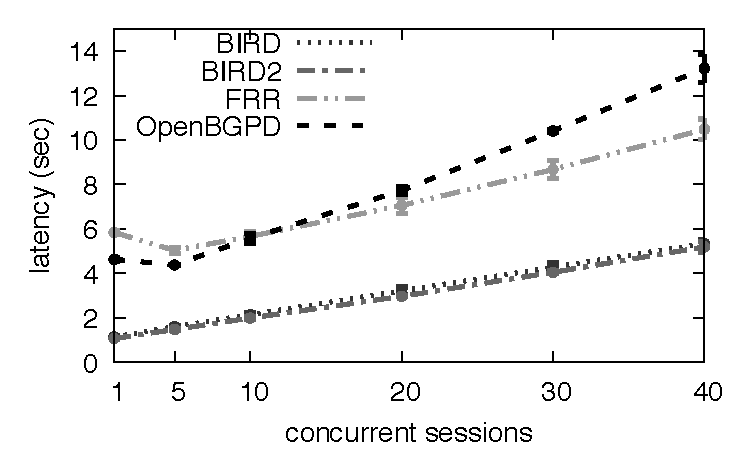
\includegraphics[width=\linewidth]{images/table-transfer-scalability.pdf}
	\captionof{figure}{Table transfer latency (800k).}\label{fig:tbl-transfer-scalability}
\end{minipage}
\begin{minipage}[c]{.49\linewidth}
	\centering
	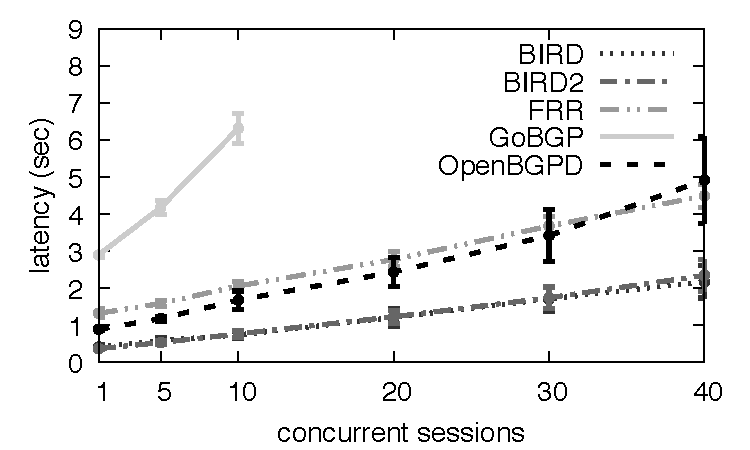
\includegraphics[width=\linewidth]{images/ssbt-scalability.pdf}
	\captionof{figure}{Route update latency (50k). } \label{fig:ssbt-scalability}
\end{minipage}

\hfill

\begin{minipage}[c]{.49\linewidth}
	\centering
	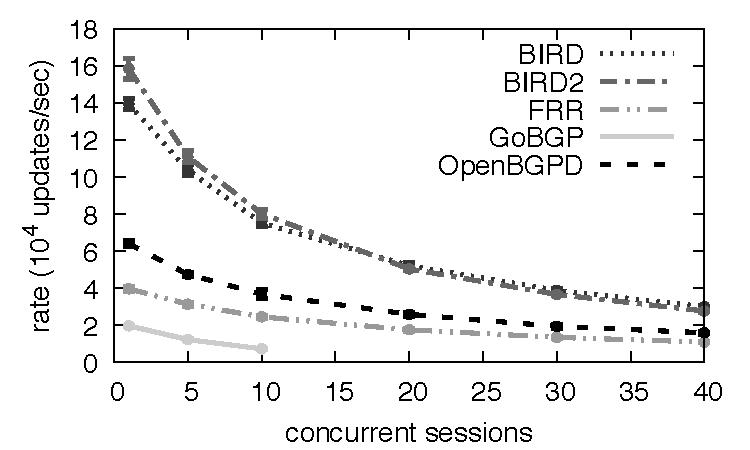
\includegraphics[width=\linewidth]{images/ssrt-scalability.pdf}
	\captionof{figure}{Single-session burst rate.}\label{fig:ssrt-scalability}
\end{minipage}
\begin{minipage}[c]{.49\linewidth}
	\centering
	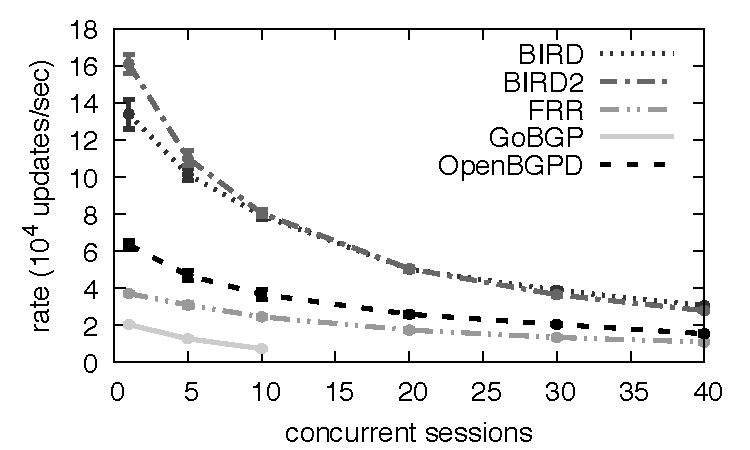
\includegraphics[width=\linewidth]{images/msrt-scalability.pdf}
	\captionof{figure}{Multi-session burst rate.} \label{fig:msrt-scalability}
\end{minipage}
\vspace{1em}

Firstly, we highlight that all speakers exhibit a very significant performance reduction as
the number of active sessions increases. This behaviour is consistent in
table transfer, update burst and continuous rate measurement scenarios.
BIRD and BIRD2 appear to experience a significant processing rate reduction for high sessions numbers, since their processing rate halves as we increase the number of sessions from 1 to 10.
Nonetheless, this performance impact is not similar in the latency measurement and both speakers exhibit a sub-linear performance decrease.
OpenBGPD and FRR exhibit a sub-linear decrease in their performance for both latency and rate measurements. These characteristics might be explained either by the employed lookup structures, which increases its lookup times for large route counts, or the internal processing scheduling mechanism.
Secondly, for all BGP speakers BGP performance varies only slightly when route updates are spread across multiple sessions.
Across all speakers there a minor performance decrease on the order to 1\%-2\% on the average route processing rate. This highlights that while all systems manage gracefully large update bursts coming from multiple parallel sessions, such as may occur during major route instabilities, however none of them manage to leverage the opportunity for parallelization to actually improve performance.
\section{Related Work}\label{sec:related}

BGP performance is a well studied problem by the measurement community.  The
majority of the studies focuses primarily on understanding the protocol-related
impact in performance critical situations, like route flapping, and only
a small set of studies have explored the BGP speaker performance
characteristics.
One of the first measurement studies on the topic~\cite{Agarwal2004}, correlated SNMP CPU route data and RouteViews dumps to
measure the data plane performance of production edge routers. Their analysis
concluded that on average BGP processing consumes approximately 60\% of the
total CPU utilization, and that a strong correlation existed between
significant CPU spikes and major BGP incidents, like the SQL Slammer worm outbreak.

Specific to the topic of performance characterisation, the IxNetwork platform
offers commercial support for BGP protocol compatibility and performance
testing \cite{ixia2004}. Using the Ixia traffic generator, Jasinska and
Malayter \cite{Jasinska2010} demonstrated significant variability in CPU
utilization between production software BGP speakers. Of great relevance to our
effort, Feldmann \textit{et al.}\cite{feldmann2004} presented a multi-dimensional study on
the factors affecting production BGP routers. Using a custom testbed equipped
with hardware-accelerated traffic generating and capturing devices, they study
the impact of the background CPU, the session count and the BGP load on the
processing latency of individual messages. Their results highlighted that the
BGP processing performance of a hardware router can increase in the order of
seconds. Similarly, Wu \textit{et al.}\cite{wu2007} developed a series of BGP interaction
scenarios to measure the impact of control and data traffic on the performance
of the BGP speaker across different platforms (CPU, NPU, ASIC).  Unfortunately,
in both studies the measurements offer limited reproducibility, since they rely
on hand-crafted measurement scenarios and specialized hardware.

    \chapter{Experimentation}

% \chapter{Characterising BGP Speaker Performance with Kakapo}

% \textbf{`kakapo'} is the name given to the project element which is concerned with performance testing.
% As such, the source code repository \url{https://github.com/hdb3/kakapo} holds the core `kakapo applications', but the repository also contains a wide range of related elements, including the orchestration framework, `kagu', and even some other, non-performance related resources, including the PIR/BGP protection evaluation infrastructure.
% And, since `kagu' even downloads, builds and bundles the Haskell BGP applications which form the core of the implementation work undertaken for this thesis, the `kakapo' repo is a starting point to reproduce and replicate all work reported here.

\section{Motivation, and BGP Speaker Performance Models}

\subsection{A Model of BGP System Performance}

\subsubsection*{Application Model}
As a network software system, a BGP speaker might be expected to behave in somewhat predictable fashion: if, as is usually the case, the BGP endpoint is running in a conventional operating system context, we can expect that the TCP support is based on OS level code rather than a custom TCP stack.
BGP is a rare exception in that it often uses the obscure TCP authentication method, (RFC 2385 - Protection of BGP Sessions via the TCP MD5 Signature Option), however Linux has long had support for this feature.
How widely used it is unclear (cite: https://labs.ripe.net/author/andrew-gallo/production-deployment-of-tcp-authentication-option/), however, it seems that a `serious' BGP implementation should be capable of it.
Which makes `custom' TCP stacks even less accessible.
However, the integration between TCP and BGP is rather special, in the sense that the use of TCP flow control to interact with BGP as an application level pacing scheme is historically important (see/ ref `slow peer' elsewhere in the thesis.)

BGP itself is message based, even though TCP is stream based, therefore any BGP implementation implements a message level recovery system over the received TCP stream, while the OS is expected to be responsible only for assembling the aggregate of line level TCP segments into larger buffers visible to the client application.
Therefore, we can expect that a BGP implementation might be sensitive to \textit{BGP} message level overheads, which it cannot mitigate/offload, while TCP stack support for large buffers might mean that system call overhead can be minimised.
Since a full Internet table at protocol level is at most around 10-20 MB, even a large update burst of 10,000 prefixes might be 100 kbytes, and thus easily fit into a single read buffer when read via system-call.
Of course, an eager BGP might read very greedily, and thus use more system calls than strictly necessary, however this would be poor design, and most likely under load even such a design would fall back to more efficient behaviour, unless an independent thread were allocated to the task.
This area is one which the multi-peer kakapo tests can illuminate.

`A further expectation of any BGP speaker is that there is some degree of per BGP message processing, and that that overhead is independent of the core function of prefix level table work.
Therefore, if differences in performance can be observed when the same table content is organised as packed prefixes or not packed, then it can shine light on the aspects of performance bottlenecks in an underlying implementation.
It might even be possible to characterise different implementations of BGP, and thus identify actual usage of these implementations based solely on MRT stream data.
This analysis of BGP system motivates the kakapo test parameters provided, i.e. table size, and group size, which are applicable to both continuous and burst mode tests, and burst size which is applicable to only burst mode testing.
An analogous parameter is used to configure continuous mode testing: the window size.
A special switch to enable unpacked routes is also provided by kakapo, applicable to all test modes.

\subsubsection*{Target System Architecture Model}
In each measured case of a BGP speaker, the target system is a software implementation of the same underlying application function.
The performance of such a system can be predicted using a complexity analysis model.
This model defines the processing load and resulting execution time as a function of the input data's size.
Ideally, for a BGP speaker, execution times would depend linearly, at worst, on key dimensions of input data size.
A straightforward model can be constructed by associating a weight or cost with each dimension.
This model then attempts to predict measured performance based on a linear relationship with each factor.
It is also reasonable to expect that in real systems with features like CPU caching, small-scale scenarios might perform anomalously fast.
This behaviour would likely stabilise above a certain size threshold.
Therefore, several experiments can be designed to investigate each of the anticipated complexity factors.
Of course, it may be that the performance function is a linear in any single factor, but multilinear overall.
That is one question which may be answered by these experiments!

% \chapter{Characterising BGP Speaker Performance with Kakapo}


\section{Kakapo: A Methodology for BGP Performance Measurement}
The general experimental architecture consists of a single experimental subject system with connected BGP peers, acting as sources and sinks for BGP messages.
The connected peers are logically distinct, as far as the subject is concerned.
The Update message sources are the main source of experimental variation, although even the Update sinks may be sources of variation, for example, in their number, and their ability to accept output from the subject without blocking at the transport (TCP) level.
The experimental observations consist principally of the timing, content and ordering of BGP output messages, of which content is prescribed by configuration and stimulus, so that only timing aspects are in general measurable independent variables.
A secondary variable parameter is content related - Update structure - in particular, the use of (or not) prefix packing, where applicable.
The main simplifying assumption used, across the experiments reported, is that measurements relate solely to numbers of routes injected and exported, rather than content, for example in a burst mode experiment a fixed number of routes is injected, and the principal measurement principle is the determination of the delay before the same number of routes is emitted to a particular sink peer.
Variations exist, for example, when it cannot be guaranteed that all injected routes will be reexported, a `canary' or marker techniques is used, to indicate that all routes submitted have been processed.


\textbf{`kakapo'} is the name given to the project element which is concerned with performance testing.
As such, the source code repository \url{https://github.com/hdb3/kakapo} holds the core `kakapo applications', but the repository also contains a wide range of related elements, including the orchestration framework, `kagu', and even some other, non-performance related resources, including the PIR/BGP protection evaluation infrastructure.
And, since `kagu' even downloads, builds and bundles the Haskell BGP applications which form the core of the implementation work undertaken for this thesis, the `kakapo' repo is a starting point to reproduce and replicate all work reported here.

\paragraph{Continuous Rate Measurement}
Continuous rate measurement is another variation - in continuous measurement there are always Updates `in flight', and therefore no well define duration, or set of durations, so the observation is of rate rather than duration, but the principle remains of correlation between submitted load by count, and detected numbers re-exported, based only on the number, rather than any inspection of content.
\footnote{a continuous measurement variation based on injection or marking of specific timestamped messages in the flow, and their subsequent later arrival timestamp has been attempted, but the complexities of the scheme were such that reliable measurements were not achieved.
However, it was observed that some BGP speakers have a tendency to slow down or even stall during extended test execution, therefore, for future work, it would be of real value to complete the development of a framework capable of measuring Update processing latency and latency variation.}
Note that, because packing usage is not always consistent, the measured counts must be of routes (individual prefixes), rather than Update messages and therefore BGP Paths.\footnote{in early experimentation this was a source of difficulty, when it was discovered that one BGP speaker frequently `degenerated' under load into a state in which prefix grouped 
updates were being broken into larger numbers of smaller Updates.
Until that time the measurement  procedure was much simpler, and relied on message (Update) counts, rather than prefix (route) counts.}

\paragraph{Message Burst Duration Measurement}
At the lowest level of observation there are more than two events which can be used as duration delimiters: on the sending side there are two events - the time of first transmission, as seen at the network link level, and the time of transmission of last related message.
Similarly, on the subsequent downstream link, there are two distinctive events - the times of first and last transmission.
To complicate matters further, strictly one might distinguish the beginning and end of transmission on the link for a single burst, and, perhaps more material, there are transport protocol aspects, and it may be more meaningful to determine the end of a transmission as the point at which the last sent data has been acknowledged at the transport level.
Were the measurements to be made based on packet capture then at least we could specify which events are defined as the recognised start and end points; however, in the majority of reported experimentation here the measurement of time and thus duration is made in the sending or receiving application, i.e. in this case `kakapo'.
kakapo is a regular Linux network socket based application, and the methodology used to collect timestamps, and thus duration, is as follows: on transmission, the start time is defined as the system timestamp before the first socket write call is made on transmission, the end time is defined as the system timestamp after the transmit TCP buffer has become empty, which is believed to represent the state reached when a TCP level acknowledgement has been received for all data written to the socket \footnote{in the kakapo/core application the source file is txwait.c, in which the buffer state is retrieved using the ioctl 
system call SIOCOUTQ.
The txwait() function polls this API at 100uS intervals until it reduces to zero.}
On reception the procedure is simpler - the receive loop processes all BGP messages via a common function \footnote{bufferedRead() in session.c}, and buffered read executes socket read() as required, and whenever socket read() is called productively and successfully, a timestamp is recorded.
This timestamp is used in the Update message processing for both rate and burst mode tests, to define the time at which a message was received.
There is no explicit record kept of arrival of first data/Update during any test procedure, however, by setting low values of burst size, for example, a burst of one block, it is possible to the latency of single messages.
Capturing the unrecorded `time-to-first-message' for burst mode tests could be considered for future work, however from the standpoint of evaluating a BGP implementations `fitness-for-purpose' it was not considered to be a significant parameter, by comparison with measures of time to complete operations.
As already mentioned, there are cases in which the 'end of reception' cannot be reliably measured for the main Update stream alone.
In these cases an special 'canary' route Update is sent, after the main stream, and the measured duration is based on timestamps captured for the canary, using the same underlying system call strategy.
In practice therefore, there are three variables of interest which are consistently recorded for burst tests: time sending starts time sending ends (last sent Update acknowledged at transport level) time receiving ends Of these, the interval duration between sending start and receiving end is the most significant from a `fitness-for-purpose'.
It is noteworthy that at least some other work has used the 'end-of-sending' to define duration of processing - clearly, this risks serious under estimation of actual time to complete, and the under-estimate is highly material, since the functional value of a routing protocol is on delivered when either routes are propagated down-stream, or, when the local forwarding plane has been updated to reflect the latest t routing state.
Since in most experiments conducted here, there is no forwarding plane to observe, this BGP message level analysis is the most relevant as well as only approach applicable.

\paragraph{Measurables}
In summary, the primary experimental measurables are the duration interval between staring transmission of a burst, the end of transmission, and the end of subsequent re-transmission downstream.
Additional observational values of interest may include resource utilisation, for example CPU load, or dynamic system memory allocation.
Ad-hoc recording of these secondary parameters is included in some experimental reports, and some instrumentation for the purpose has been deployed, however time prohibits the systematic presentation of these secondary observables.
Highly related however are the measurement of performance made as system CPU and memory resource limits were varied in the container hosting the target BGP systems.
Complementing the burst measurement duration based independent variables is the rate based rate independent variable.
This is a simpler measure, consisting merely of a single record of start and end of a continuous traffic test, where the start and end are measured identically to the burst case, but additionally, the total recorded number of received routes is counted and recorded.
The resulting measurement is given as rate, where the actual underlying observables, duration and route count or Update message count, are also reported.


% Original heading: \subsubsection*{Experimental Control Variables}
\subsection{Kakapo - Control and Configuration}
The primary observable results of BGP performance were described already in the previous section - principally they are:

\begin{myitemize}
    \item burst duration - time re-announce
    \item burst duration - time to accept
    \item rate mode - continuous state update message rate
    \item initial table transfer duration (variant of burst duration)
\end{myitemize}

There is a much wider range of control variables available for experimentation than there is of independent variables.

\bigskip

Control variables can be categorised by class:
Direct Experimental Variables
Target/Subject Variables
Platform Environment Variables

\paragraph{Direct Experimental Variables}

Direct Experimental Variables define an experimental context, independent of the measurement target - it should be possible to apply a set of Direct Experimental Variables to a range of target BGP platforms, and compare the outcomes case-by-case.
The categories of Direct Experimental Variables are as follows (a listing of the corresponding application parameters used by kakapo is given in the following table \ref{tab:kakapo_cp}).
\begin{itemize}
    \item underlying full table structure - i.e. the number of routes (prefixes), and the number of distinct paths (sometimes also confusingly called `routes').
    \item the size, structure and content of a burst of Update messages - where  it is implicit that the burst represents a subset of the full table, albeit with often with variation in some path-attribute, such that an earlier sent version of a route will be updated and thus trigger re-announcement
    \item for continuous mode rate-measurement, the main mode specific test parameter is the transmit window size
    \item number of source peers - more than a single source peer may be connected; the source peers might each originate a full route table, or, only the aggregate of announcements may amount to a single copy of a full route table; multiple connected peers may remain active during the measurement phase, i.e. in turn or interleaved multiple peers may originate burst or continuous streams which are measured - or, after an initial conditioning phase involving multiple source peers, only a single source peer may be used to originate measured bursts or streams.
    \item number of sink peers - a BGP speaker must do some additional work in order to support multiple peers, even when those peers are only in an experimental context receivers of routes rather than originators.
    \item Multiple sinks is a rather important criteria in any `fitness-for-purpose' evaluation, for the trivially obvious reason that in most real-world core IDR contexts there are multiple candidate routes for many or most routes, and therefore in a normal context arbitrary newly received routes are either announced to many peers or to none at all - so performance capacity to feed routes to many sinks is more relevant that capacity to process concurrent updates from many sources.
    \item context of measurement triggers - for example intervals between bursts, and numbers of repetitions of bursts
\end{itemize}

\paragraph{Target/Subject Variables}
Independent of \textit{Direct Experimental Variables}, \textit{Target/Subject Variables} define the target BGP system for a specific test scenario - principal Target/Subject Variables include:
\begin{itemize}
    \item identity and version of the target - e.g.
        \begin{itemize}
            \item bird (bird2)
            \item frr, version 8.2
            \item Cisco vIOS
            \item \hbgp
            \item etc. etc.
        \end{itemize}
    \item provisioned CPUs and system memory - often, prescribed by the container or virtual machine environment for the target
\end{itemize}

\paragraph{Platform Environment Variables}
Other potentially significant variables, which must at least be controlled, include:
\begin{itemize}
    \item host hardware - processor and system model, e.g.
    \item laptop, server, etc., etc.
    \item host operating system and release versions for both experimental framework and target
    \item software versions of the test framework
\end{itemize}

For Platform Environment Variables there may be less value in directly evaluating variants, but for experimental integrity it is important that they are fixed, for any given reported set of measurements, especially when making comparisons between different BGP implementations.

\subsection{kakapo control parameters}
Much of the complexity of kakapo lies in the wide variety of parameters it supports, and test mode variants.
kakapo has 26 named configuration parameters, some most significant ones are listed below.
In addition, kakapo implements a highly detailed parameter logging scheme, with around 30 distinct test parameters logged, though not all are applicable for all test modes.
A list of important kakapo control parameters and their usage is given in table~\ref{tab:kakapo_cp}.

\bigskip

\begin{longtblr}[
  caption = {\texttt{kakapo} control parameters},
  label = {tab:kakapo_cp},
]{  
  width = \linewidth,
  colspec = {X[2,l] X[2,l] X[5,l]},
  hlines,
  vlines,
  cell{1}{1} = {r=3,c=1}{c,lightgray},
  cell{5}{1} = {r=3,c=1}{c,lightgray},
  cell{5}{3} = {r=2,c=1}{l},
  cell{9}{1} = {r=3,c=1}{c,lightgray},
  cell{10}{3} = {r=2,c=1}{c},
  cell{13}{1} = {r=4,c=1}{c,lightgray},
  cell{13}{3} = {r=2,c=1}{l},
  cell{17}{1} = {r=4,c=1}{c},       
 }

Core table control 
& PATHCOUNT & Define the size of the full route table based on the number of distinct \textit{paths}.
The resulting table will have PATHCOUNT x GROUPSIZE prefix entries.
Use only one of PATHCOUNT or PREFIXCOUNT. \\ \nopagebreak

 & PREFIXCOUNT & Define the size of the full route table based on the number of distinct \textit{prefixes}.
The resulting number of paths will still be consistent with the GROUPSIZE parameter.\\ \nopagebreak

 & GROUPSIZE & Specify how many prefixes are associated with a single BGP path.
Unless explicitly disabled, this number of prefixes will always be packed into a single Update message. \\


 Mode switch 
 & MODE & There are three basic modes: FILE, RATE, MULTI, corresponding to the kakapo operational modes described in detail in the text.
Variants exist, to enable or disable certain behaviours.
\\
Table content fine-tuning options
& SEEDPREFIX & The route table is constructed using the prefix defined as  SEEDPREFIX/SEEDPREFIXLEN, e.g.
10.0.0.0/24, and continuing with the adjacent prefix, calculated using SEEDPREFIXLEN as the interval.
In the example of 10.0.0.0/24, the second prefix would be 10.0.1.0/24 \\ \nopagebreak
 & SEEDPREFIXLEN &  \\ \nopagebreak
 & CANARYSEED & Similar to SEEDPREFIX, except canaries are always /32, so there is no need for a `CANARYPREFIXLEN'.  \\ \nopagebreak

Disable packed Updates
& NOPACK & Modify the behaviour of the Update generator, but not the underlying route-table.
Every prefix will be sent in a separate Update, even if there exist other prefixes with which it could be packed. \\

Burst mode control 
& MAXBURSTCOUNT & The number of Update messages to be sent in each timed burst.
\\ \nopagebreak
& REPEAT &  \\ \nopagebreak
& REPEATDELAY &  \\
 pre-prepared route table
 & SENDFILENAME &  The named file should contain line-encoded valid BGP messages.
The file content will be transmitted en-bloc.
Responsibility of the user to provide valid content.
The `mrtdump' utility can be used to extract route tables from MRT encoded sources.\\
Rate mode controls
 & RATECOUNT & define the terminating condition for a rate test cycle, either as number of messages sent (RATECOUNT), or duration in seconds (RATETIMELIMIT).\\ \nopagebreak
 & RATETIMELIMIT &  \\ \nopagebreak
 & RATEWINDOW & Number of unprocessed Update messages which will be allowed to be outstanding. \\ \nopagebreak
 & MAXBLOCKINGFACTOR & Minimum number of updates which will be written to the socket - effectively keep the size of TCP segments low to avoid thrashing in either the client, or, kakapo.
In effect, temporarily extends the RATEWINDOW. \\ \nopagebreak


General network and protocol configuration & TCPPORT & default destination TCP port for outbound BGP connections.\\
 & PEERMAXRETRIES & limit the number of attempts in establishing initial peer connections.
kakapo will error exit if it cannot establish all of the connections it is requested to provide.
\\
 & HOLDTIME &  The hold-time value sent in bgp open message.
Kakapo correctly negotiates hold-time, but will offer zero (which disables use of BGP Keepalive).\\
 & TIMEOUT & This value is used on BGP TCP sockets as a `socket option'.
Effectively defines a liveness detection mechanism on peer connections.
Defaults to 20 seconds.
\\
\end{longtblr}

\subsection{Core Test Modes and Lifecycle}
A kakapo test cycle consists of an initial peer session establishment phase, a `conditioning' phase, a core test phase, and finally a graceful shutdown of BGP peer sessions.
The `conditioning' phase is intended to prepare the target BGP instance by announcing a full route table, thereby disregarding from experimental observations any initial software behaviour such as allocating memory for route tables.

The core test phase consists of re-announcements of routes first announced in the conditioning phase, but with different path-attributes, such that the target SUT should re-announce the routes.
During the core test phase Where more than one kakapo route source is enabled, each source peer in turn announces a block of routes, so that the load on the SUT is distributed evenly over the set of sources.\footnote{But, the conditioning phase presents a `'full' address table to each peer.}
The structure, rate and pattern of route announcements, and the number of configured route sources are all configurable, allowing a wide range of tests to be conducted.

There are two main modes of testing, burst mode and continuous mode.
In burst mode, the observed value is the duration from the start of transmission of a large block of routes to the receipt of the final re-announcement by the SUT.
Continuous mode was developed because repeated burst tests showed that BGP speaker performance could be sensitive to the delay between bursts, suggesting that single-block timing may be unrepresentative of real operational demands.
The hypothesis is that for implementations in languages using techniques like garbage collection\footnote{e.g. gobgp (golang), \hbgp (Haskell}, simple burst tests may not expose weaknesses that impact sustained loads.
Therefore, continuous mode provides a better stress and soak test.
In this mode, kakapo probes a BGP speaker with a dynamically adjusted flow to determine its sustained processing capacity.
It works by setting a `transmit window'—a number of ‘in-flight’ Update messages—and sending new updates only as re-announced updates are received, thus maintaining the window size.
A small blocking factor is used for transmissions to prevent inconsistent results caused by TCP stack overhead.
The primary observed value is the sustained rate of announcements in routes per second.


\subsection{Control Parameters - Collection and Implementation in kakapo}
The classification of experimental parameters between `Direct Experimental Variables', `Target/Subject Variables' and `Platform Environment Variables' is closely mirrored in the experimental framework - essentially, every one of the `Direct Experimental Variables' described is available as a configuration variable to kakapo, while the others cannot be set by kakapo itself; `Target/Subject Variables', e.g. target identity, allocated CPU and system memory, are controlled by the wider experimental framework , while Platform Environment Variables are constrained for a given set of experiments by the available infrastructure.
These 'environment variables' are handled simply by recording the current execution environment in the logging system.
In summary: kakapo itself \textit{sets} (and may vary over a range), Direct Experimental Variables  (the experimental framework \textit{provides} the values to kakapo, but does not itself implement them) the experimental framework \textit{directly sets} Target/Subject Variables the experimental framework \textit{discovers} Platform Environment Variables

kakapo also has the role of logging all contextual data - it does this using structured text passed in by the experimental framework.
This ensures that experimental measurements and their full context are consistently aligned in the logging record.


\subsection{Route Synthesis Methodology}

In general, the requirement for kakapo is to generate continuous or repeated burst of updates which, in aggregate, are larger than a single route table.
This necessarily requires that routes are repeated, i.e. the same prefixes used more than once.
Kakapo must also ensure that routes it generates will always be re-announced by the target BGP speaker.
In simple cases, i.e. where routes are originated by a single peer, this requirement is easily met, simply by modifying almost any route attribute, such as the source AS in the AS path list.
However, for the case that kakapo emulates multiple route source peers, the case is more complex, unless each source peer exclusively originates route for distinct sets of prefixes, because the requirement is that the most recently advertised instance of a route is always selected and thus re-advertised.
Rather consistently associate specific routes with specific peers, kakapo resolves the issue by increasing the Local Preference of routes, whenever it starts a repeat cycle for routes already announced.
This ensures that new routes from any peer are always preferred and thus re-announced downstream by the SUT.

\subsubsection{Test Topology - use of IBGP and EBGP}
This use of Local Preference as an important aspect of route synthesis has impacts on the test configuration - which must always involve at least one EBGP peering relationship, for obvious reasons, i.e., IBGP routes are not re-advertised to other IBGP peers.
Since Local Preference is only used in IBGP, it forces the overall test configuration AS level structure  - source peers must be IBGP peers to the SUT - the sink peer must be an EBGP peer to the SUT.
This constraint presents no problem for the test procedure, however it is an important aspect to the overall route synthesis design.
A related issue is that this choice of IBGP-source, EBGP-sink, simplifies the multiple-sink-peer methodology, because it ensures that the test target does not devote resources to propagating the routes it receives from one source peer to all of the other source peers, (which otherwise it would do were they configured as EBGP peers), and thus make multi-peer testing even more demanding for a test target, and less easy to draw conclusions about the effects of multiple-peer topology, than tests in which the same numbers of routes are both sent and received by the test system, where the intent is to investigate potential gains from parallel operation in cases where the work load is comparable with a test which is not so easily parallelised.\footnote{Obviously, the multiple EBGP peer topology is entirely relevant to real-world cases, and a worthy target for investigation as another experimental case.
But, this is still enabled by Kakapo using the same methodology, i.e. a test with M source peers and N sink peers is a possible experiment, albeit one which has not been carried out (yet).}

\subsubsection{\textbf{Canary routes}}
A `canary route' is a technique used to determine when route processing has been completed in the cases where some or all transmitted Updates are {\it not} re-announced, and also simply for confidence that an experimental phase has fully completed.
Since in real world operation it is often the case that received routes will not be preferred and re-announced, it is difficult to measure this outcome precisely due to the lack of a notice for the processing completion.
Canary routes are simply routes which are constructed such that they will always be propagated: typically this means that for each source peer, a different unique canary prefix is defined.
By sending a canary Update after a test burst which is not expected to be propagated, we can measure the processing delay by simply timing the delay before the canary re-emerges.
This strategy relies on the BSUT processing routes in strict sequence for a given peer, which must be independently confirmed for each BGP speaker.
All of the BGP speakers in our study did exhibit this behaviour, including those which claim or exhibit multithreaded processing capability.
Canary routes also provide a good method for troubleshooting invalid configurations - since kakapo currently does {\it not} correlate every transmitted and received messages, it uses simple counts of messages to determine when a burst has been completely received.
By transmitting a canary as the last message in a burst, kakapo can quickly detect and report when some Updates have been dropped.

\subsubsection{Comparison of Processing Performance between `Real' Internet route Tables and Synthetic Routes of Similar Size}
Kakapo by default synthesises BGP route tables, but also has a mode which uses `real' BGP route data extracted from core Internet route tables in MRT format.
Since artificial routes are widely used in this study, a comparative measurement between a `real' route table and a synthetic one was performed to validate the significance of the results.
For repeated burst tests or continuous load tests, real MRT data cannot be used directly.
The primary reason is that re-announcing the same route table will have no table change impact on a target system, and thus will not produce any output BGP messages to measure.
Furthermore, it is difficult to establish when all routes have been processed, as different BGP speakers may silently discard or choose not to re-announce certain routes, making simple message counting unreliable.
To overcome this, the `route canary technique' is used to reliably detect the end of processing.
An additional, critical limitation is that MRT data cannot be used for experiments where the route profile itself is a key variable.
If the objective is to measure how performance is affected by specific route packing structures or to use the number of routes as a control parameter distinct from the number of prefixes, MRT data is unsuitable because it has its own highly variable and uncontrollable route and prefix set values.
Fortunately, the validating experiments show good consistency between the route processing performance of synthetic and `real' data, confirming that synthetic data can be used for in-depth investigations without loss of significance.

\subsection{Logging and Data Traceability}
The logging system is a vital aspect of kakapo.
kakapo itself writes only to local file system (the capability to write to network resources exists in the codebase, but has been deprecated in favour of orchestrator directed log management.)

During extended execution, kakapo may write many intermediate logs, but the most important ones are start and finish logs, and an exceptional exception log written when kakapo terminate abnormally.
The main purpose  of the logging system is to record experimental results, but equally important is the record of the associated control parameters which apply to a particular test run - without a record of all parameters, the experimental record cannot be put into it correct specific context.
The applicable context is also important - kakapo records a range of specifics, for example the host name of the system on which the test runs, the data and time, the versions of all software components in use - and, where execution context is a laptop, the power source in use at the time of the experiment.
Finally, in addition to the parameters measured or known to kakapo, there is an additional capability to add further metadata in the log records, data which is supplied by the orchestration framework.
Examples are tags to allow specific sets of observations to be easily extracted and analysed in isolation, and some other parameters which kakapo cannot monitor or control, for example, CPU and memory resource limits applied to the system-under-test and its Docker container.

\subsubsection{kakapo logging, integrity, reproducibility and traceability}
kakapo logging enables an important experimental  objective, which is the safeguarding of the integrity of experimentation and accumulated raw data.
It provides a strong basis for validating claims and conclusions made in reports.
All of the experimental data reported in this thesis is available, online, for inspection and further analysis, or to reproduce existing  tables and graphs.
The archived form is structured JSON, which can be used directly with the reporting tools developed and used to produce most of the graphs and tables in the thesis, although in general a MongoDB database has been used to aggregate the data during the development and experimentation process.

\subsubsection{kakapo event log format and types}
Depending on test mode (burst or continuous), and running time, kakapo writes at least two event records, and in some longer running cases a number of intermediate records.
A special further event log type is used for exceptional termination of a test run, for example when peer stops responding or closes a peering association, or on some internal kakapo events, or signalled early exit.
The most important event type is the summary record, which is written at the end of an execution cycle, and which is the basis for most reports and graphs.
The summary record contains most of the control parameters which are also written in a start record, which is the other main event log type.
Start records are most useful for diagnosing the cause of unsuccessfully test runs, than for analysing the results of successful runs.
A sample summary log record is shown below.

\subsubsection{kakapo centralised log management}
kakapo itself simply writes valid JSON objects, serially, into a log file.
The resulting log file is not strictly valid JSON, requiring only open and close brackets to make valid.
The current methodology for aggregating and safeguarding kakapo log data is to write the logs periodically into a MongoDB NoSQL database.
This approach conveniently deduplicates records, and allows data from different hosts and times to be safely and simply aggregated, with no immediate need for manual intervention.

\section{Performance Evaluation and Results}

\section{Baseline BGP Performance}

Baseline measurements of BGP performance target the central scale factors of complex BGP deployments: route table size---measured in terms of numbers of paths, prefixes, and source peers. A BGP speaker's software tables scale directly with these parameters.

\subsection{Key Questions}

Valid enquiries are:
\begin{itemize}
    \item How long does it take for the target system to process the routes it receives?
    \item Once it has built the tables, do these scale factors affect its ability to perform routing operations?
\end{itemize}

Related questions address how the structure of routing updates affects processing capacity and performance. Specific questions to be explored include:
\begin{itemize}
    \item Does initial table transfer time scale linearly with the number of peers?
    \item Are bursts handled as quickly when multiple active peers are connected?
    \item Are continuous mode measurements consistent with burst mode?
    \item Do different BGP implementations have different performance envelopes depending on the measurement criterion (initial table, burst, rate)?
\end{itemize}

\section{Test Programmes}

\subsection{Initial Table Transfer}
For each target platform, measure the time taken to process a full route table:
\begin{itemize}
    \item as the route table varies in total size (measured by prefixes and paths).
    \item as the route table structure varies in terms of paths, holding table size constant.
    \item as the group size (number of prefixes per announcement) varies, holding the number of paths constant.
\end{itemize}

\subsection{Effect of Update Packing}
Repeat the initial table transfer measurements while disabling the packing of prefixes and compare the results.

\subsection{Stable State, Burst Processing Performance}
Measure the duration of processing bursts of updates of varying sizes. Repeat these measurements with variations in the route structure, using a subset of the values from the initial transfer tests.

\subsection{Rate-Based Measurements}
In each scenario where burst performance has been measured, substitute a continuous stream of updates.

\subsection{Effect of Multiple Peers}
Repeat a subset of all the above measurements in scenarios with multiple active source peers.

\subsection{Sensitivity to Experimental Parameters}
Explore sensitivity to experimental parameters, such as:
\begin{itemize}
    \item rate window size.
    \item burst repetition interval duration.
\end{itemize}

\section{Analysis and Hypotheses}

\subsection{General Expectations}
\begin{itemize}
    \item Larger inputs are expected to take more time to process, but the relationship should be no more than linear.
    \item With a larger installed routing state (table size, number of peers), burst and rate mode measurements might show a performance decline. However, this decline should be sub-linear if the software structure is moderately well designed.
    \item There may be multiplier effects between, for example, the number of peers and the size of the route table.
\end{itemize}

\subsection{Packing and Update Structure}
\begin{itemize}
    \item Route tables with fewer paths (larger group size) might yield better performance. However, there could be trends in both directions: large groups may require more work to construct announcements (poorer performance), while also reducing message-level overhead such as parsing (better performance).
    \item If packing is disabled, the performance for tables with a high group size is expected to decline to the performance of a table composed entirely of singletons (assuming such tables perform worse). This might lead to the conclusion that only the prefix count matters, apart from the gain accruing from reduced overhead in iterating over fewer Update messages.
    \item Distributing load (burst or continuous) over multiple peers is expected to improve performance if the target system has concurrent processing capabilities. If not, some mild disadvantage might be observed when working with loads over multiple peers.
\end{itemize}

\section{Test Framework: Kakapo, Kagu, and Forest}

For most of the proposed experiments, each `data point' represents a single invocation of the \texttt{kakapo} core binary application and an instance of the target BGP speaker. The \texttt{kagu} framework provides the orchestration of the various BGP instances (usually, as \texttt{Docker} containers).

Part of \texttt{kagu}/\texttt{kakapo} is an experiment configuration template system named \texttt{forest}. The complete workflow is as follows:
\begin{enumerate}
    \item \texttt{forest} takes a \texttt{YAML} file that defines the range of parameters needed, along with any invariants. The output of \texttt{forest} is a series of shell commands that drive the \texttt{kagu} runtime framework. Each command line differs from the others only in the parameters set to vary, for example, the \texttt{table-size} and the target BGP speaker.

    \item \texttt{kagu} is invoked once for each line in the script file. It builds the needed network interfaces and address mappings for the BGP systems it will start. It then constructs the \texttt{Docker} commands (or \texttt{libvirt/virsh}) to start the BGP endpoints---one is always a \texttt{kakapo} container, the other varies depending on the BGP target named in the command line. \texttt{kagu} transcribes the parameters directed at \texttt{kakapo} (for example, the table size) into the command parameters that \texttt{kakapo} needs, which are then passed explicitly into the \texttt{Docker} container. By careful crafting, the BGP platform-specific configuration files need not be changed for any of the experiments.

    \item \texttt{kakapo} is run as a container in the foreground rather than as a daemon, which allows it to control the experimental lifecycle. It executes the configured test and exits when complete, or on error. \texttt{kakapo} is started with a logging file mapped into the container; this file records the progress and results of the instance. \texttt{kakapo} sets signal handlers that allow it to exit gracefully, even if an exception arises in its own code.
\end{enumerate}

This process allows for the management of very long-running experiments, even in the event of system outages. \texttt{forest} scripts can be restarted because they contain sequence numbers that are recorded in the logging file. As long as the host file system is not corrupted, no experimental data can be lost.


% Baseline measurements of BGP performance target the central scale factors of complex BGP deployments:
% route table size - measured in terms of numbers of paths, numbers of prefixes and numbers or (source) peers.
% A BGP speaker of necessity has software tables that correspond to directly in scale to these parameters.

% Valid enquiries are:
% \begin{itemize}
%     \item how long does it take for the target system to process the routes it receives
%     \item once it has built the tables, do these scale factors affect its ability to perform routing operations?
% \end{itemize}

% Related questions address how the structure of routing requests affect the processing capacity and performance in completing those requests.

% Concrete test programs:

% Initial table transfer

% for each target platform, measure the time taken to process a full route table
% \begin{itemize}
%     \item as the route table varies in total size (measured by routes~prefixes)
%     \item  as the route table structure varies in terms of paths
%     \item \begin{itemize}
%      \item  holding table size constant
%     \item  holding group size constant
%     \end{itemize}
% \end{itemize}

% Effect of Update packing

% Repeat and compare the same measurements, whilst disabling packing of prefixes.

% Stable state, burst processing performance

% measure the duration of processing bursts of updates of varying sizes.
% repeat the measurements with variations in the route structure (using some subset of the values in part 1)

% Effect of multiple peers
% Repeat some subset of all of the above measurements, in scenarios with multiple active source peers.
% Does initial table transfer time scale linearly?

% Are bursts handled as fast, when multiple active peers are connected?

% Rate based measurements

% In each scenario in which burst performance has been measured, substitute continuous mode.
% Are the continuous mode measurements consistent with burst mode?
% Do the different BGP implementations have different performance envelopes depending on the measurement criterion (initial table, burst, rate.)

% Sensitivity to experimental parameters
% explore
% - sensitivity to rate window size
% - to burst repetition interval duration

% Analysis, Hypotheses
% We should expect that larger inputs generally take more time to process, but no more than with linear relation.
% We might expect that having a larger installed routing state (size of table, number of source peers), that burst and rate mode measurement show some variation (performance decline).  But sublinear, if the software structure is even moderately well designed.
% We might expect that their are multiplier effects between, for example numbers of peers and size of route table.

% Packing and update structure
% We might expect that route tables with fewer paths (larger group size) have better performance, but there could be trends in both directions, e.g. large groups may require more work to construct announcements, leading to poorer performance, while the same variation might contribute to better performance in the area of processing where there is a message level overhead, for example in parsing an update, and in reducing the size of a `path table', if such a thing exists in the target implementation.
% We might expect that if packing is disabled that the performance for high group size tables declines to the performance of an all singleton table (assuming that such tables do have worse performance.)
% This might lead to the conclusion that only prefix count matters, excepting the `trivial' gain accruing from reduced overhead in iterating over more Updates.
% We might also expect that distributing load (burst or continuous), over multiple peers, would lead to better performance, if, and only if, the target system has some concurrent processing capability - but if, not then perhaps some mild degree of disadvantage when working with loads over multiple peers.

% Configuring and Analysing Results In A Kakapo Test Campaign
% For most of the proposed experiments, each `data point' represents a single invocation of the kakapo core binary application, and also of an instance of the target BGP speaker.  The kagu framework provides the orchestration of the various BGP instances (usually, as Docker containers).

% kagu, kakapo and forest

% Part of kagu/kakapo is an experiment configuration template system which builds a sequence of test scripts which in aggregate represent the tests needed.  The tool is `forest' - the complete picture is as follows:
% forest takes a yaml file which defines the range of parameters needed, and also any invariants -the output of forest is a series of command lines (Linux shell commands) which drive the kagu runtime framework.  Each line differs only from the others in the batch in the parameters which are set to vary - for example, the table-size, and the target bgp speaker.
% kagu is invoked once for each line in this script file - kagu builds the needed network interfaces and address mappings for the BGP systems that it will start, and then constructs the Docker commands (or libvirt/virsh) which will start the BGP endpoints - one of them always a kakapo container, the other varies, depending on the BGP target named in the command line.  kagu transcribes the parameters which are directed at kakapo (for example, the table size) - into the command parameters that kakapo needs.  These are passed into the Docker container explicitly by kagu.  In this way, kakapo is configured and started, as a container, along with the target BGP speaker (BGP speakers each have there own configuration files, but by careful crafting, these BGP platform specific files need not be changed for any of the experiments known to kagu and forest).
% Although Kakapo is run as container, it is run in the foreground rather than as a daemon, this allows kakapo to control the experimental lifecycle.  Kakapo executes the configured test, and exits when complete, or on error or exception, terminating the container.  Kakapo is started with a logging file mapper into the container, and this updated file records the progress and results of the experimental instance, including when kakapo exits (kakapo sets signal handlers which allow it to gracefully exit, even if the exception arises in its own code.)

% Forest scripts can even be restarted, because they contain sequence numbers, and the sequence numbers are recorded in the logging file.  The procedure is manual, but trivial, and allows very long running experiments to be managed, even in the event of system outages.  And, of course, as long as the hist file system is not corrupted, no experimental data can be lost.

\section{Reported Experimental Program}

In the interest of space and relevance, only a limited selection of experimental reports is given.

\paragraph{The first report} corresponds to the initial findings during the development of both kakapo and \hbgp.
It is the measurement of initial transfer duration for some `representative' sized routing tables, followed by the simple measurement of burst performance, in the context of this specific `representative'  route table.

In the initial work, the range of BGP speakers was limited (no Cisco or Junos virtual routers), and older versions of almost every BGP platform than reported here.  It's noteworthy that gobgp in particular is now demonstrably more mature, in that it is now possible to conduct most measurements, whereas in earlier times gobgp could not be reliably tested with full route tables and loads such as these.

Here are the `forest' YAML files which define these initial experiments \footnote{`forest' did not exist when these experiments were first conducted, however another orchestration system was in use - Haskell based (`forest' is Python!  The Haskell framework was not so easy to use and modify.) }

This is the content of the `forest' YAML file for the first experiment: \inputminted{yaml}{specs/burst1.yaml}


At the risk of stating the obvious, the specification requests that a set of experiments be conducted using the bgp speakers bird1, bird2, bird3, frr, hbgp, bgpd, gobgp, relay, with a route table size of 800000 (prefixes).
The meaning of the remaining lines is as follows:

\verb|  MAXBURSTCOUNT: "10000"|
\verb|MODE: SINGLE| - kakapo experiment mode is defined here
\verb*|  REPEAT: "5"| instructs that the burst test should be executed 5 times,
\verb|spec: forest| is a signature line - the `forest' script will reject the input of it is missing.

There are two comment lines - 
\begin{verbatim}
  # GROUPSIZE: 1..10
  # NOPACK: 0,1    
\end{verbatim}

which are placeholders for hopefully obvious variations on the file for a future similar experiment, and the remaining non-comment lines are tags of sorts which do not affect the experiment, but help to track and distinguish the recorded data for later analysis.

The script forest transforms this YAML file into the following lines of Linux shell script:
% \begin{adjustbox}{max width=\textwidth}
% { \fontsize{6pt}{9.6pt}\selectfont
% \begin{lstlisting}
\begin{lstlisting}[basicstyle=\fontsize{10pt}{16pt}\selectfont\ttfamily]


    

SEQ=0 SPEC=burst1 TAG=EXAMPLE_burst1 REPEAT=5 MAXBURSTCOUNT=10000 PREFIXCOUNT=800000 MODE=SINGLE target=bird1 /home/nic/kakapo/testing/smoketest/runx.sh
SEQ=1 SPEC=burst1 TAG=EXAMPLE_burst1 REPEAT=5 MAXBURSTCOUNT=10000 PREFIXCOUNT=800000 MODE=SINGLE target=bird2 /home/nic/kakapo/testing/smoketest/runx.sh
SEQ=2 SPEC=burst1 TAG=EXAMPLE_burst1 REPEAT=5 MAXBURSTCOUNT=10000 PREFIXCOUNT=800000 MODE=SINGLE target=bird3 /home/nic/kakapo/testing/smoketest/runx.sh
SEQ=3 SPEC=burst1 TAG=EXAMPLE_burst1 REPEAT=5 MAXBURSTCOUNT=10000 PREFIXCOUNT=800000 MODE=SINGLE target=frr /home/nic/kakapo/testing/smoketest/runx.sh
SEQ=4 SPEC=burst1 TAG=EXAMPLE_burst1 REPEAT=5 MAXBURSTCOUNT=10000 PREFIXCOUNT=800000 MODE=SINGLE target=hbgp /home/nic/kakapo/testing/smoketest/runx.sh
SEQ=5 SPEC=burst1 TAG=EXAMPLE_burst1 REPEAT=5 MAXBURSTCOUNT=10000 PREFIXCOUNT=800000 MODE=SINGLE target=bgpd /home/nic/kakapo/testing/smoketest/runx.sh
SEQ=6 SPEC=burst1 TAG=EXAMPLE_burst1 REPEAT=5 MAXBURSTCOUNT=10000 PREFIXCOUNT=800000 MODE=SINGLE target=gobgp /home/nic/kakapo/testing/smoketest/runx.sh
SEQ=7 SPEC=burst1 TAG=EXAMPLE_burst1 REPEAT=5 MAXBURSTCOUNT=10000 PREFIXCOUNT=800000 MODE=SINGLE target=relay /home/nic/kakapo/testing/smoketest/runx.sh

\end{lstlisting}

% \end{adjustbox}

 Fortunately for the reader, there is only one range parameter in this input, and the range is small, resulting in just eight script lines.
 But, when the comment lines\begin{verbatim}
  # GROUPSIZE: 1..10
  # NOPACK: 0,1    
\end{verbatim}

are converted to active configuration - 

\begin{verbatim}
  GROUPSIZE: 1..10
  NOPACK: 0,1    
\end{verbatim}

Then the resulting script will have 160 lines, and may take rather longer to execute than this version.

We now show the output in the console, and later some fragments of the structured log file, arising from executing these scripts.

(Incidentally, this complete set of experiments executes in around 5 minutes.
The fastest BGP speaker runs in 31 seconds, the slowest, gobgp, takes a little more than one minute.  bird2, the next fastest, takes 32 seconds, although it is still 10x slower than the fastest, our reference BGP, `relay'.  Even though gobgp now completes most tasks, it is still much the slowest of all of the `software' BGPs (Cisco and Juniper VMs will be discussed later.))

With only a few lines redacted, here is the complete console log of one of the execution cycles, in this particular case the BGP target was FRR.

\begin{figure}[H]
\begin{adjustbox}{}

\begin{lstlisting}[numbers=left]
kakapo  version: 1.0-743-g876b50d  built: Tue Jun  3 05:55:51 UTC 2025  branch: main
connecting from 172.18.0.19 to 172.18.0.13:45824 (179) (0)
connecting from 172.18.0.20 to 172.18.0.13:45824 (179) (0)
connection initiated for 2 peers

BGP Open: as = 64504, routerid = 172.18.0.13 , holdtime = 180, opt params = 0206010400010001020280000202020002024600020641040000fbf8020206000206450400010101020a490806616c656630310002044002c0780209470700010180000000
BGP Open: as = 64504, routerid = 172.18.0.13 , holdtime = 180, opt params = 0206010400010001020280000202020002024600020641040000fbf8020206000206450400010101020a490806616c656630310002044002c0780209470700010180000000
connection complete for 2 peers
conditioning start
conditioning:          peer 1 64504:172.18.0.20
conditioning complete: peer 1 64504:172.18.0.20  elapsed time 4.360066
conditioning complete: elapsed time 4.403960
canary for peer 1 64504:172.18.0.20
canary_all complete: elapsed time 0.050753
cycle 0
single_peer_burst_test total elapsed time 0.513073 count 100000 (transmit 0.005274) (receive 0.512899)
canary for peer 1 64504:172.18.0.20
canary_all complete: elapsed time 0.050711
cycle 1
.........

..........
cycle 4
single_peer_burst_test total elapsed time 0.508013 count 100000 (transmit 0.010109) (receive 0.507823)
canary for peer 1 64504:172.18.0.20
canary_all complete: elapsed time 0.050845
single_peer_burst_test mean=0.494902 max=0.522436 min=0.474067
Notification complete: elapsed time 0.000143
notification complete for 2 peers
kakapo exit
killed frr
\end{lstlisting}
\end{adjustbox}
\end{figure}
% BGP Open: as = 64504, routerid = 172.18.0.13 , holdtime = 180, opt params = 0206010400010001020280000202020002024600020641040000fbf8020206000206450400010101020a490806616c656630310002044002c0780209470700010180000000
% BGP Open: as = 64504, routerid = 172.18.0.13 , holdtime = 180, opt params = 0206010400010001020280000202020002024600020641040000fbf8020206000206450400010101020a490806616c656630310002044002c0780209470700010180000000

Some commentary: 
AT line 1 we see the kakapo start log output, with its version information (this will also be found in the structured log file)
At lines 6-8 the BGP peer associations that have been formed.  kakapo doesn't understand what the BGP Open options mean, but it can be given a special instance to send, if required.
At lines 9-12 we see the conditioning phase, i.e. the initial table transfer .
An additional interesting measurement here is the transmit time for each BGP peer, which is present in the log, for each BGP peer in turn, but the console is only reporting an aggregate, and we see here the total duration, from start of sending to end of receiving the re-announcement of the initial table for all peers.
At lines 13-14 the canary route exchange is reported - arguably canary here is redundant, but it is used widely to give confidence that each experimental stage has been completed.  Canaries are single routes.  Note that, for FRR, the smallest transaction always takes around 50 mS, because of all BGPs, FRR is the only one which does not disable Nagle.
At lines 19, the real `test' starts, and the number of cycles are as requested in the forest configuration. 
The report shows two numbers - (transmit 0.005274) (receive 0.512899) -  which added compose the aggregate - 0.513073.  As noted, FRR never takes less than 50mS for any transaction, so, for FRR, with this request size - 10,000 routes - the experiment is in some sense void.
The more relevant datum is the initial transfer time - 4.3 seconds - which is one of the slowest in the pack.   

We now show the structured log entry which was generated from this test cycle:

\begin{lstlisting}[    numbers=left]

    {
        "type": "summary",
        "unixtime": 1749509284,
        "elapsed_time": 36.951536,
        "test_name": "single_peer_burst_test",
        "time": "2025-06-09 22:48:04.412000",
        "sender_count": 1,
        "conditioning_duration": 4.17579,
        "mean": 0.486382,
        "max": 0.517761,
        "min": 0.474661,
        "sd": 0.01814,
        "PATHCOUNT": 80000,
        "PREFIXCOUNT": 800000,
        "GROUPSIZE": 10,
        "MAXBURSTCOUNT": 10000,
        "REPEAT": 5,
        "NOPACK": 0,
        "RATECOUNT": -1,
        "RATETIMELIMIT": 20,
        "single_rate": 0,
        "multi_rate": 0,
        "BRANCH": "main",
        "VERSION": "1.0-743-g876b50d",
        "HOSTNAME": "tauben",
        "UUID": "03ba4f38-445d-4eed-a8fe-57c7f79f697f",
        "exit_status": "NOT SET",
        "target": "frr",
        "TAG": "EXAMPLE_burst1",
        "SEQ": "8",
        "SPEC": "burst1",
        "N_PEERS": "1",
        "PSU_STATUS": "AC",
        "DOCKER_NCPUS": "16",
        "DOCKER_MEMORY": "96g",
        "WINDOW": 5000
    },
\end{lstlisting}

This record holds all of the relevant context of a test run, as well as the test control parameters and measured values.
The additional data is the environment and results.
For example, we can see that this run was in a Docker environment with 96G bytes of system memory and 16 CPUs.
Kakapo is not smart enough to choose which results to report depending on what test mode, so the meaning full data here is in the fields

\verb|"conditioning_duration": 4.17579|

\verb|"mean": 0.486382|

\verb|"max": 0.517761|

\verb| "min": 0.474661|

\verb| "sd": 0.01814|

 while
 
 \verb| "single_rate": 0|
 
 \verb| "multi_rate": 0,|
 
 are zero because the test was not a rate test.

 Every test run has a unique UUID, so that other records can be correlated with the final `summary' record, e.g., records such as start, and intermediate records that contain the measurements for each run, rather than just the means logged here.  Most other fields are self explanatory, e.g. `host' and `time'.


\section{Experimental Data Reporting and Presentation}

Previously, the methodology for definition and collection of experimental data was described, which consists of structured data sets in which most of the collected data values are `met-data' context for core experimental measurement values.

In order to effectively report and analyse this data, some form of automation is required.
The approach developed is described here.

\paragraph{Reporting Requirements}
The usual objective in reporting is to produce some form of graphical display, or a summary table, highlighting the relevant control variables and resulting experimental observations.
Since data is collected into a general pool, part of the requirement is to isolate and extract data records which are relevant to the topic; equally important for experimental integrity is to ensure that only directly comparable data is used in a single report, for example, that only data collected on a certain server, or in a certain experimental context, is used in a single report.


A side-effect of the selection phase is a summary of the metadata which is held fixed for the selected data, for example, the host name of the system used for the experiment, and any control parameters which are single valued for this report.  The metadata could also include the date ranges over which the data was collected, and software versions of any components in the experiment.


Once a valid subset of data values is isolated, the next objective is to construct the sets of index values - usually control parameters - and to form a regular representation of the measurements values, e.g., an n-dimensional matrix of measurements, in which index values are the `unit vectors' for the value matrix.

An intermediate step to forming this value matrix is the reduction of measurements from selected records to single data values: this may have two aspects:
\begin{enumerate}
    \item select which single value of several semantically distinct measurements present in the record
    \item summarise, e.g. calculate a mean (average), or some other format, such as an error-box structure
\end{enumerate}

Note, if more than one type of measurement is present in the data records, then this may also be interpreted as a dimension in the value matrix, for example when rate data is collected, each measured rate record also contains the measured duration for the `conditioning phase' of the experimental cycle. This could be used simply to create distinct graphs/reports, but if the complementary data should be plotted in the same report, then it should be processed as a dimension in this way.


Once this data reduction stage is complete a regular data structure is in hand, and the choices of graph ranges and axes labels etc are implicitly already determined, so that a graph or table is almost completely defined - the remaining task is to specify the graph or table type to apply, for example, line graphs or bar charts, etc.  The choices available may be restricted by the axes types, in particular, line graphs are only applicable to axes which are numeric, otherwise a bar chart may be a more meaningful format.
Therefore, in many cases the choice of graph form may already be implicit in the data selected.

\subsection{Reporting Implementation}
The foregoing analysis presents the requirements for a concrete framework for processing experimental data.  In this document the tool presented is a set of python scripts.  Earlier work utilised Haskell based approach, but the required graphical back end was based on libraries which have since fallen put of active development, so when the transition to JSON and MongoDB for data processing was developed a switch to python and `matplotlib' was also undertaken.  The report and graph generating framework is now part of the `kakapo' ecosystem, under the heading kakapo/report.

kakapo/report (`reports', hereafter), follows the structure set out already, i.e.

\begin{itemize}
    \item data ingestion (file or mongodb)
    \item data-set analysis and pre-processing
    \item
    \begin{itemize}
     produces a list of raw experimental data objects
    \end{itemize}
    \item dataset selection (and metadata summary preparation)
     \begin{itemize}
     \item produces a matrix structure with aligned axes vectors, the values are still raw experimental data objects
    \end{itemize}
    \item 'projection' phase
    \begin{itemize}
     \item reduce the structure raw data values to graphable values
     \item NB the projection may produce another data matrix dimension
    \end{itemize}
    \item rendering
    \item \begin{itemize}
     produce graphs or tables, using formats inferred or specified.
\end{itemize}
\end{itemize}

\subsubsection{Implementation Details}
\paragraph{Filters and Selectors}
Filters are rules (predicates) which partition the dataset, only the included elements (predicate=true) are considered for later processing.
Selectors define values used as axes values - they are rules which applied to values produce scalar values, either labels (strings), or numeric values.

In most cases, selectors and filters are simple functions which match or extract on keys in the raw data items.
Such filters most often takes key and a list of values, or a single value, while simple selectors most often take just a key.
But a selector might take a list of values as an inclusive or exclusive condition.
The fundamental difference between a filter is the output is boolean, which the selector is a value of type determined by key.
What they have in common is a key and, possibly empty, lists of inclusive or exclusive elements.
Even a filter could have empty lists, in which case the filter is on the presence (or absence) of the key itself.
The presence (or absence) of the key itself is always an implicit part of the function, and an absent key is a special value.
, for a filter it should be defined, but if there is an inclusive list in the filter then the key must be present, unless a null value is in an inclusion list.

Selectors and filters which do not fit this framework of working with keys and unprocessed values other than as equality candidates can be considered: but they are always of the form of predicate in the case of filters, or a function with a regular return type.  At this level, there is no real distinction between Filters and Selectors except that a filter should only return boolean values.  The class of such filters and selectors can be further subdivided - the simpler category being functions over a single key, while more general cases might depend on many keys in the raw data object.

\paragraph{Projectors}
At this point, the topic of projectors becomes relevant: a projector has been defined as an extractor of `y' values - and it is clear that Projectors share properties of Filters and Selectors.  The more significant distinctions being that they yield values which may be more complex than Filters and Selectors, and that, for some cases, the projector is required to implement an aggregation function.

Specifically, a Projector may have two sub-functions - 
\begin{enumerate}
    \item extract a numeric(?) value from a raw data object
    \item combine multiple extracted values to form a single `plottable' `y-value'
\end{enumerate}

 In reality, these functions can be treated independently, and the term Projector limited to the function which extracts values from raw data objects.  In this case, the Projector is much like Filters and Selectors in that simple cases can be just a key label which yields the corresponding value, and more complex cases follow the same lines as for Filters and Selectors, i.e. functions over single values, and functions over multiple values.

\paragraph{Aggregators}
 This leaves the final category of report function, which is the Aggregator.  An Aggregator may commonly be a function such as mean, sum, max or min, or even count; first, last, latest might be possible, but only if the Projector produces a structured value which for example, has a date field.  What it has always is a mapping from a type [T] to a type T.

\paragraph{ Combining Filters, Selectors, Projectors and Aggregators}

 Filters are candidates for combination, however the mechanism is ambiguous when more than one Filter is named: should AND or OR be used to combine them?  It is easy (in python, and other languages) to create a filter as a lambda of two filters, the problem comes when the member filters contain lists, and the requirement is to give the list as a command line parameter, or otherwise independent of the source code of the script.  The simplistic solution adopted is that when filters are aggregated, the implied meaning is that only elements matching every filter are passed.

 Selectors are simpler than Filters - A Selector always has a role, it may be just one of `X selector', `group selector' or `subgroup selector'.  There may at most one of each.  `group selectors' or `subgroup selectors' are optional.

 Similarly with Projectors and Aggregators, there be exactly one of each.  When a Projector produces two values, then the Aggregator is assumed to be applicable to both. [Could be made more flexible.]

 
\subparagraph{Projectors that produce multiple values}
 Projectors that produce multiple values create an implicit group or sub-group in the dataset.  The Projector defines the labels used for the subgroup itself.

\subsubsection{ Using the framework for real data and analysis}
 Until now, Filters, Selectors, Projectors and Aggregators are described in abstract terms - in practice, how should they be constructed and used?
 In practice a single combination of Selectors, Projectors and Aggregators may be applicable to a wide range of data, and thus many combinations of Filters.  Therefore, although Filters are logically relate to Selectors, Projectors and Aggregators, there usage diverges: and the divergence is reflected in the user interface; combinations of Selectors, Projectors and Aggregators are lumped into a class and concept called `view' (View objects).  View objects are widely reused, and also serve as a vehicle for carrying other data needed to construct graphs.  For a given type of View object there may be only a single applicable rendering into a graph, and certainly there can be some default prescribed as part of the View.

 Using Filters
 Evidently, a View may be a source-code level entity, while a Filter might be 'source-code' too, but one constructed dynamically rather than as a source-code literal.  For may cases, a sufficient filter specification can be defined as just a single predicate against a metadata field such as TAG or SPEC, possibly further restricted by naming a single host from which the data should be drawn.  Therefore, an invocation of a report generator may have the form:

\verb| $ report <data source> view=view1 filter=TAG=BURST1|

 or 
 
\begin{lstlisting}
$ report <data source> view=rate1 filter=TAG=RATE1,RATE2 filter=host=server1 filter=target=bird2,frr,hbgp
\end{lstlisting}
 where rate1 has been defined as:
\begin{lstlisting}

 {
  Selectors: {
    X: sender_count
    group: target
    subgroup: WINDOW
  }
  Projector: multi_rate
  Aggregator: mean
  Graph: G_line_1
 }
\end{lstlisting}

\subsection{ Report Management}
 The report tool produces graphs or tables on demand, based on command line filters and other directives.
 It is useful to easily save a report for posterity, with metadata, so that it may be repeated and validated, or reapplied when additional experimental data is available.
 The report tool facilitates this by creating archives on request, the archive contains the command used to create the plot, the figure generated, the associated metadata, and the selected raw data which formed the basis of the report.

 The effect is that any quoted result can be traced back to the original data, and the plot regenerated exactly, or run again with later data using the save command.

 An example will serve to illustrate the usage - here the data produced using the previously described experiment specification in the `forest' tool is displayed in graphical form.
 The forest specification file contained a `TAG' value, which we can use to extract just the data produced for that request.  The command line to do this is:

\begin{lstlisting}
$ ./report2.py mongo tag=EXAMPLE_burst1 opt=bar save
\end{lstlisting}
 and the resulting output (slightly truncated)I is this:

\begin{lstlisting}
Debug filter
filter recent reject_count=851 accept_count=100441 except_count=0
filter exclude_targets reject_count=93 accept_count=101199 except_count=0
filter filter_on_tags reject_count=101224 accept_count=68 except_count=0
End - Debug filter
*** rejected 101224/101292!!!

===================
Post Filter Summary
===================
summarising 68 items
sample data time window is 2025-06-10 - 2025-06-11
key: test_name [single_peer_burst_test(67)]
key: PREFIXCOUNT [800000(67)]
key: GROUPSIZE [10(67)]
key: BRANCH [pathcount(39), experimental(24), forest(2)]
key: VERSION [1.0-746-gd06d05d(48), 1.0-747-g6edd416(7), 1.0-748-gdf37aea(3), 1.0-749-ga63b427(3), 1.0-743-g876b50d(2)]
key: HOSTNAME [alef01(67)]
key: target [frr(10), bird1(8), bird2(8), bird3(8), hbgp(7), bgpd(7), relay(6), gobgp(6)]
key: TAG [EXAMPLE_burst1(67)]
key: SPEC [burst1(67)]
key: BURSTSIZE [10000(67)]
===================
***no missing cells!!!
*** duplicate cells in {'7 repeated x in relay:10', '8 repeated x in bgpd:10', '8 repeated x in hbgp:10', '9 repeated x in bird1:10', '9 repeated x in bird3:10', '7 repeated x in gobgp:10', '9 repeated x in bird2:10', '11 repeated x in frr:10'}
*** 8 elements in plot (raw=68) (@project_y)
 graph was saved to /tmp/tmptbem1tzv.png
command line was "./report2.py mongo tag=EXAMPLE_burst1 opt=bar save"
command line was ./report2.py mongo tag=EXAMPLE_burst1 opt=bar save
save dir is  /home/nic/.kakapo/1750178719

\end{lstlisting}    

 Notice from the first few lines that the database itself contains 101292 records, of which only a very few match the tag given - `EXAMPLE_burst1'.

 The generated graph \ref{fig:1750178719} for this simple experiment and analysis is shown here.

 \begin{figure}[H]
    \centering
    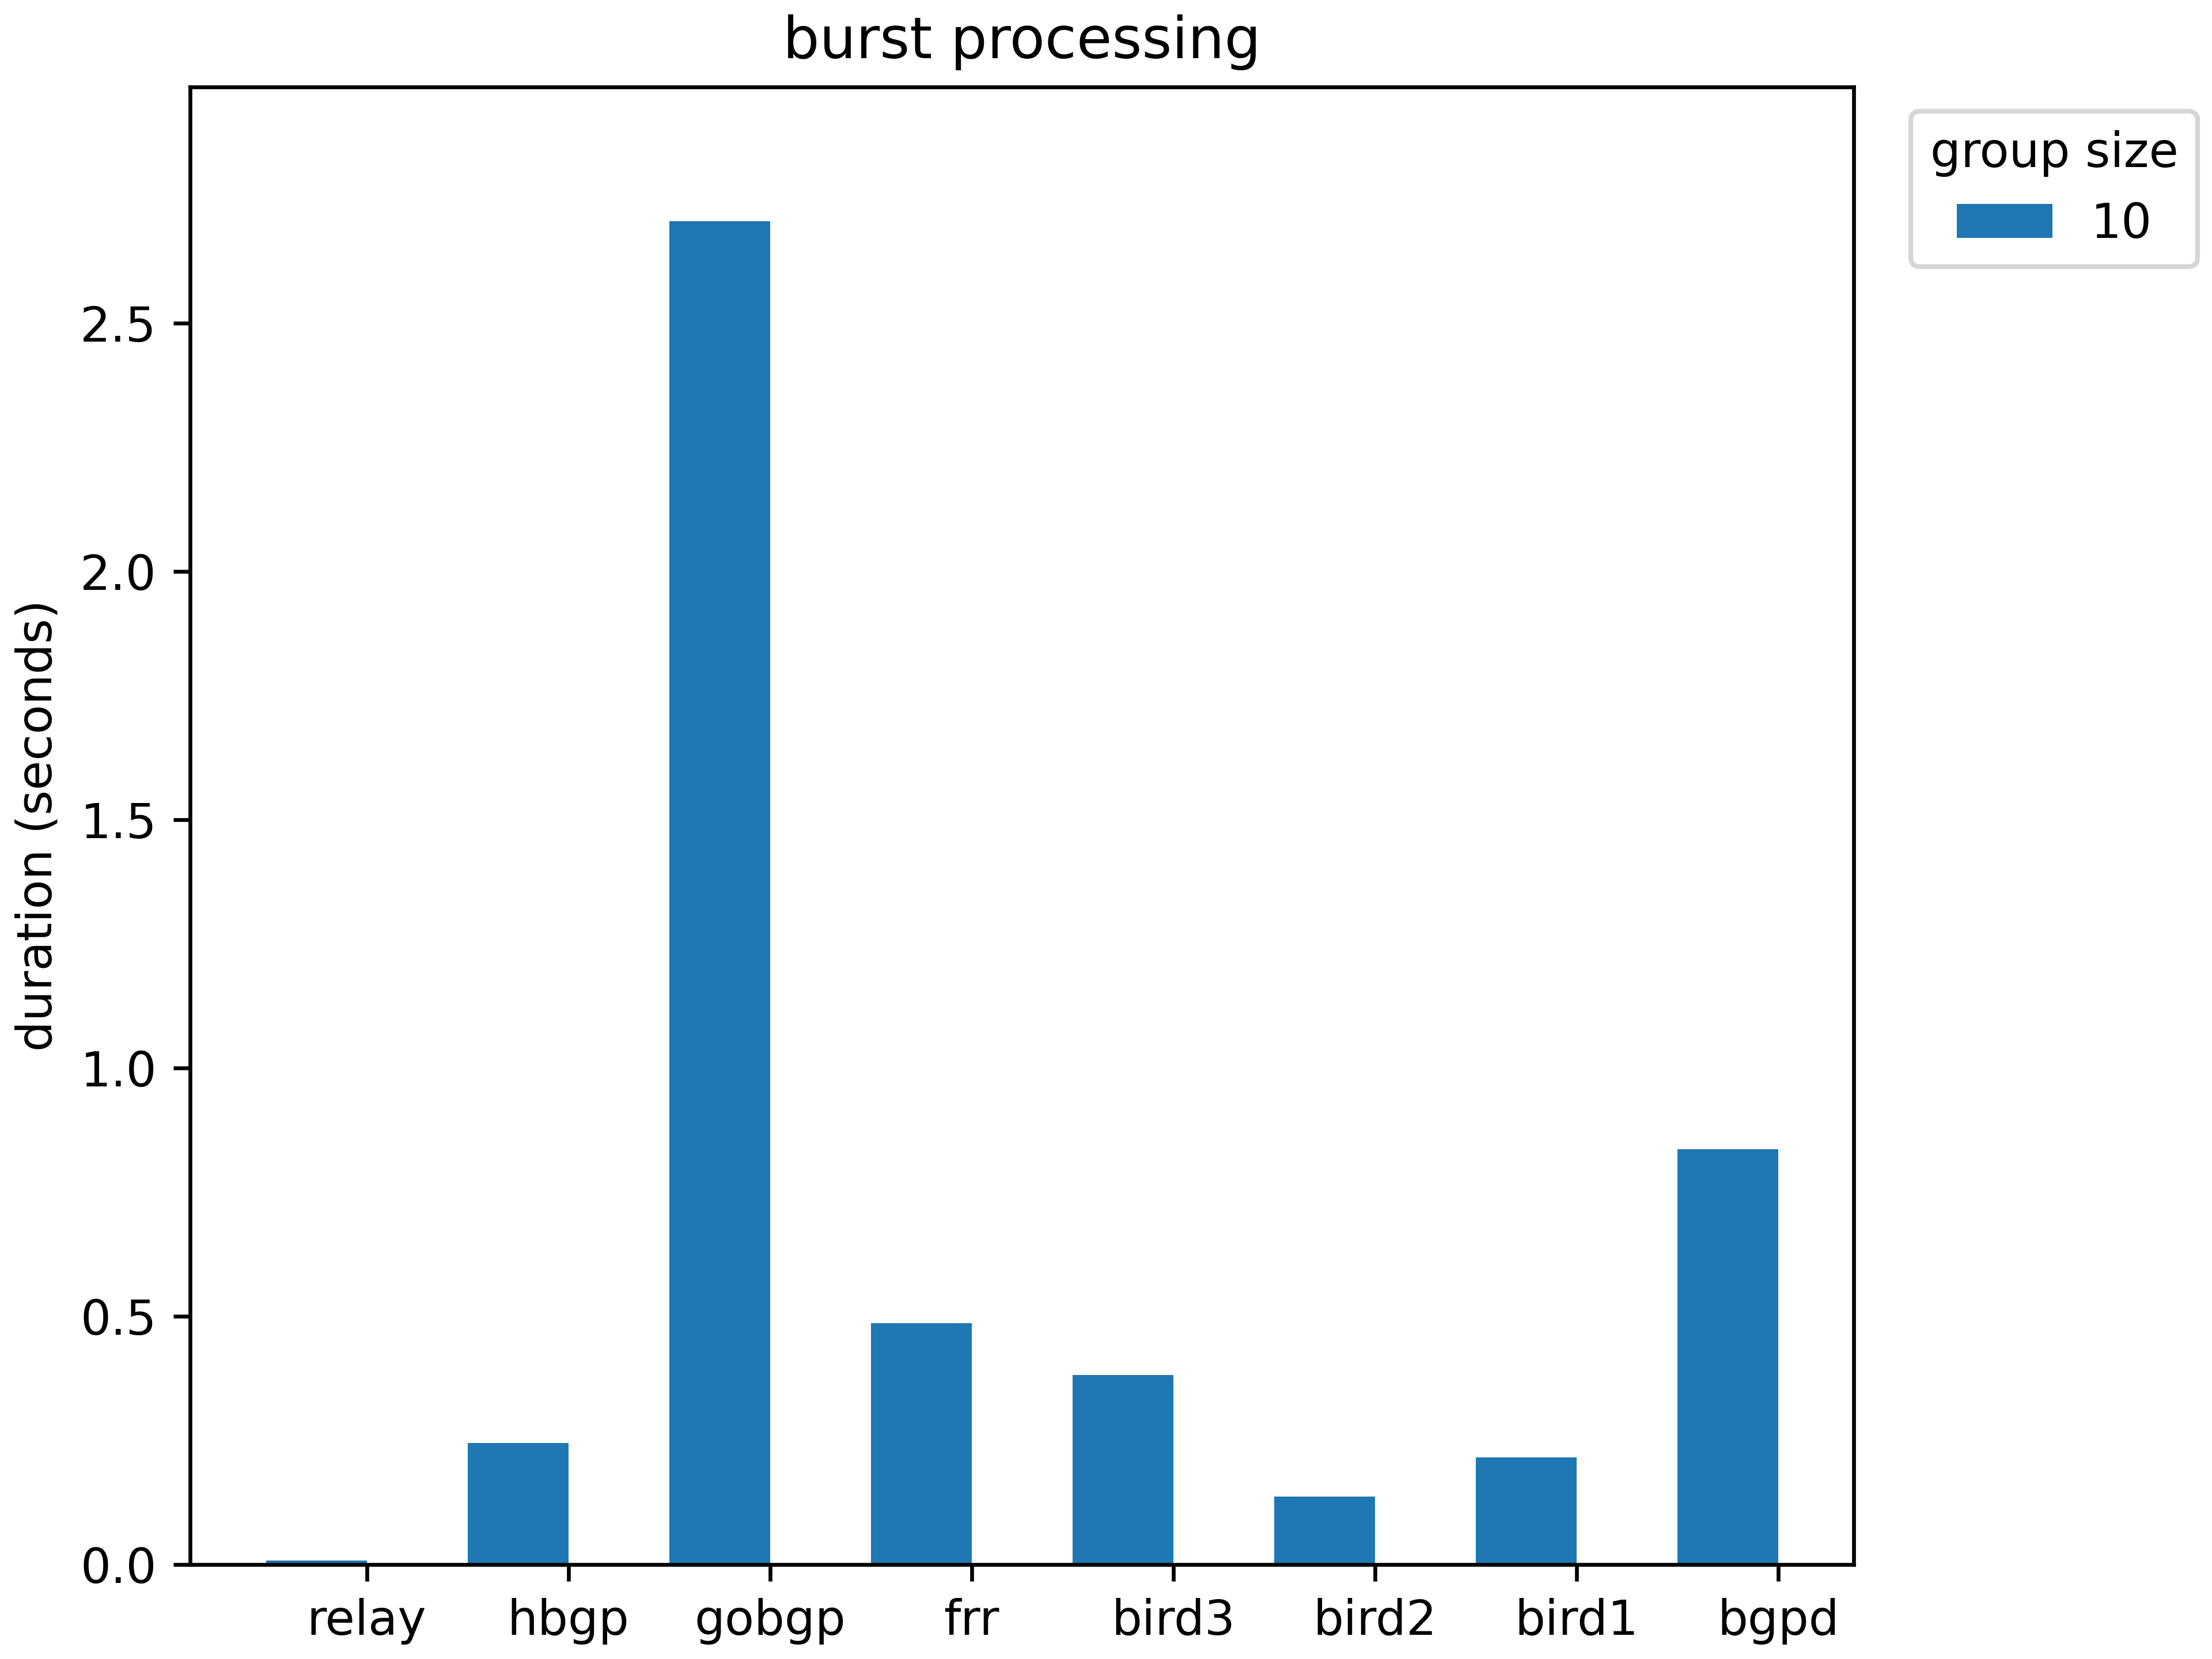
\includegraphics[width=0.7\linewidth]{1750178719.png}
    \caption{sample figure from report tool}
    \label{fig:1750178719}
\end{figure}

A more complete example is this one: \ref{fig:1750175110}.
for which the command was:
    \begin{lstlisting}
    ./report2.py mongo host=alef01 tag=samples3 targets=bird1,bird2,bird3,frr,hbgp,bgpd,gobgp save
    \end{lstlisting}

  \begin{figure}[H]
    \centering
    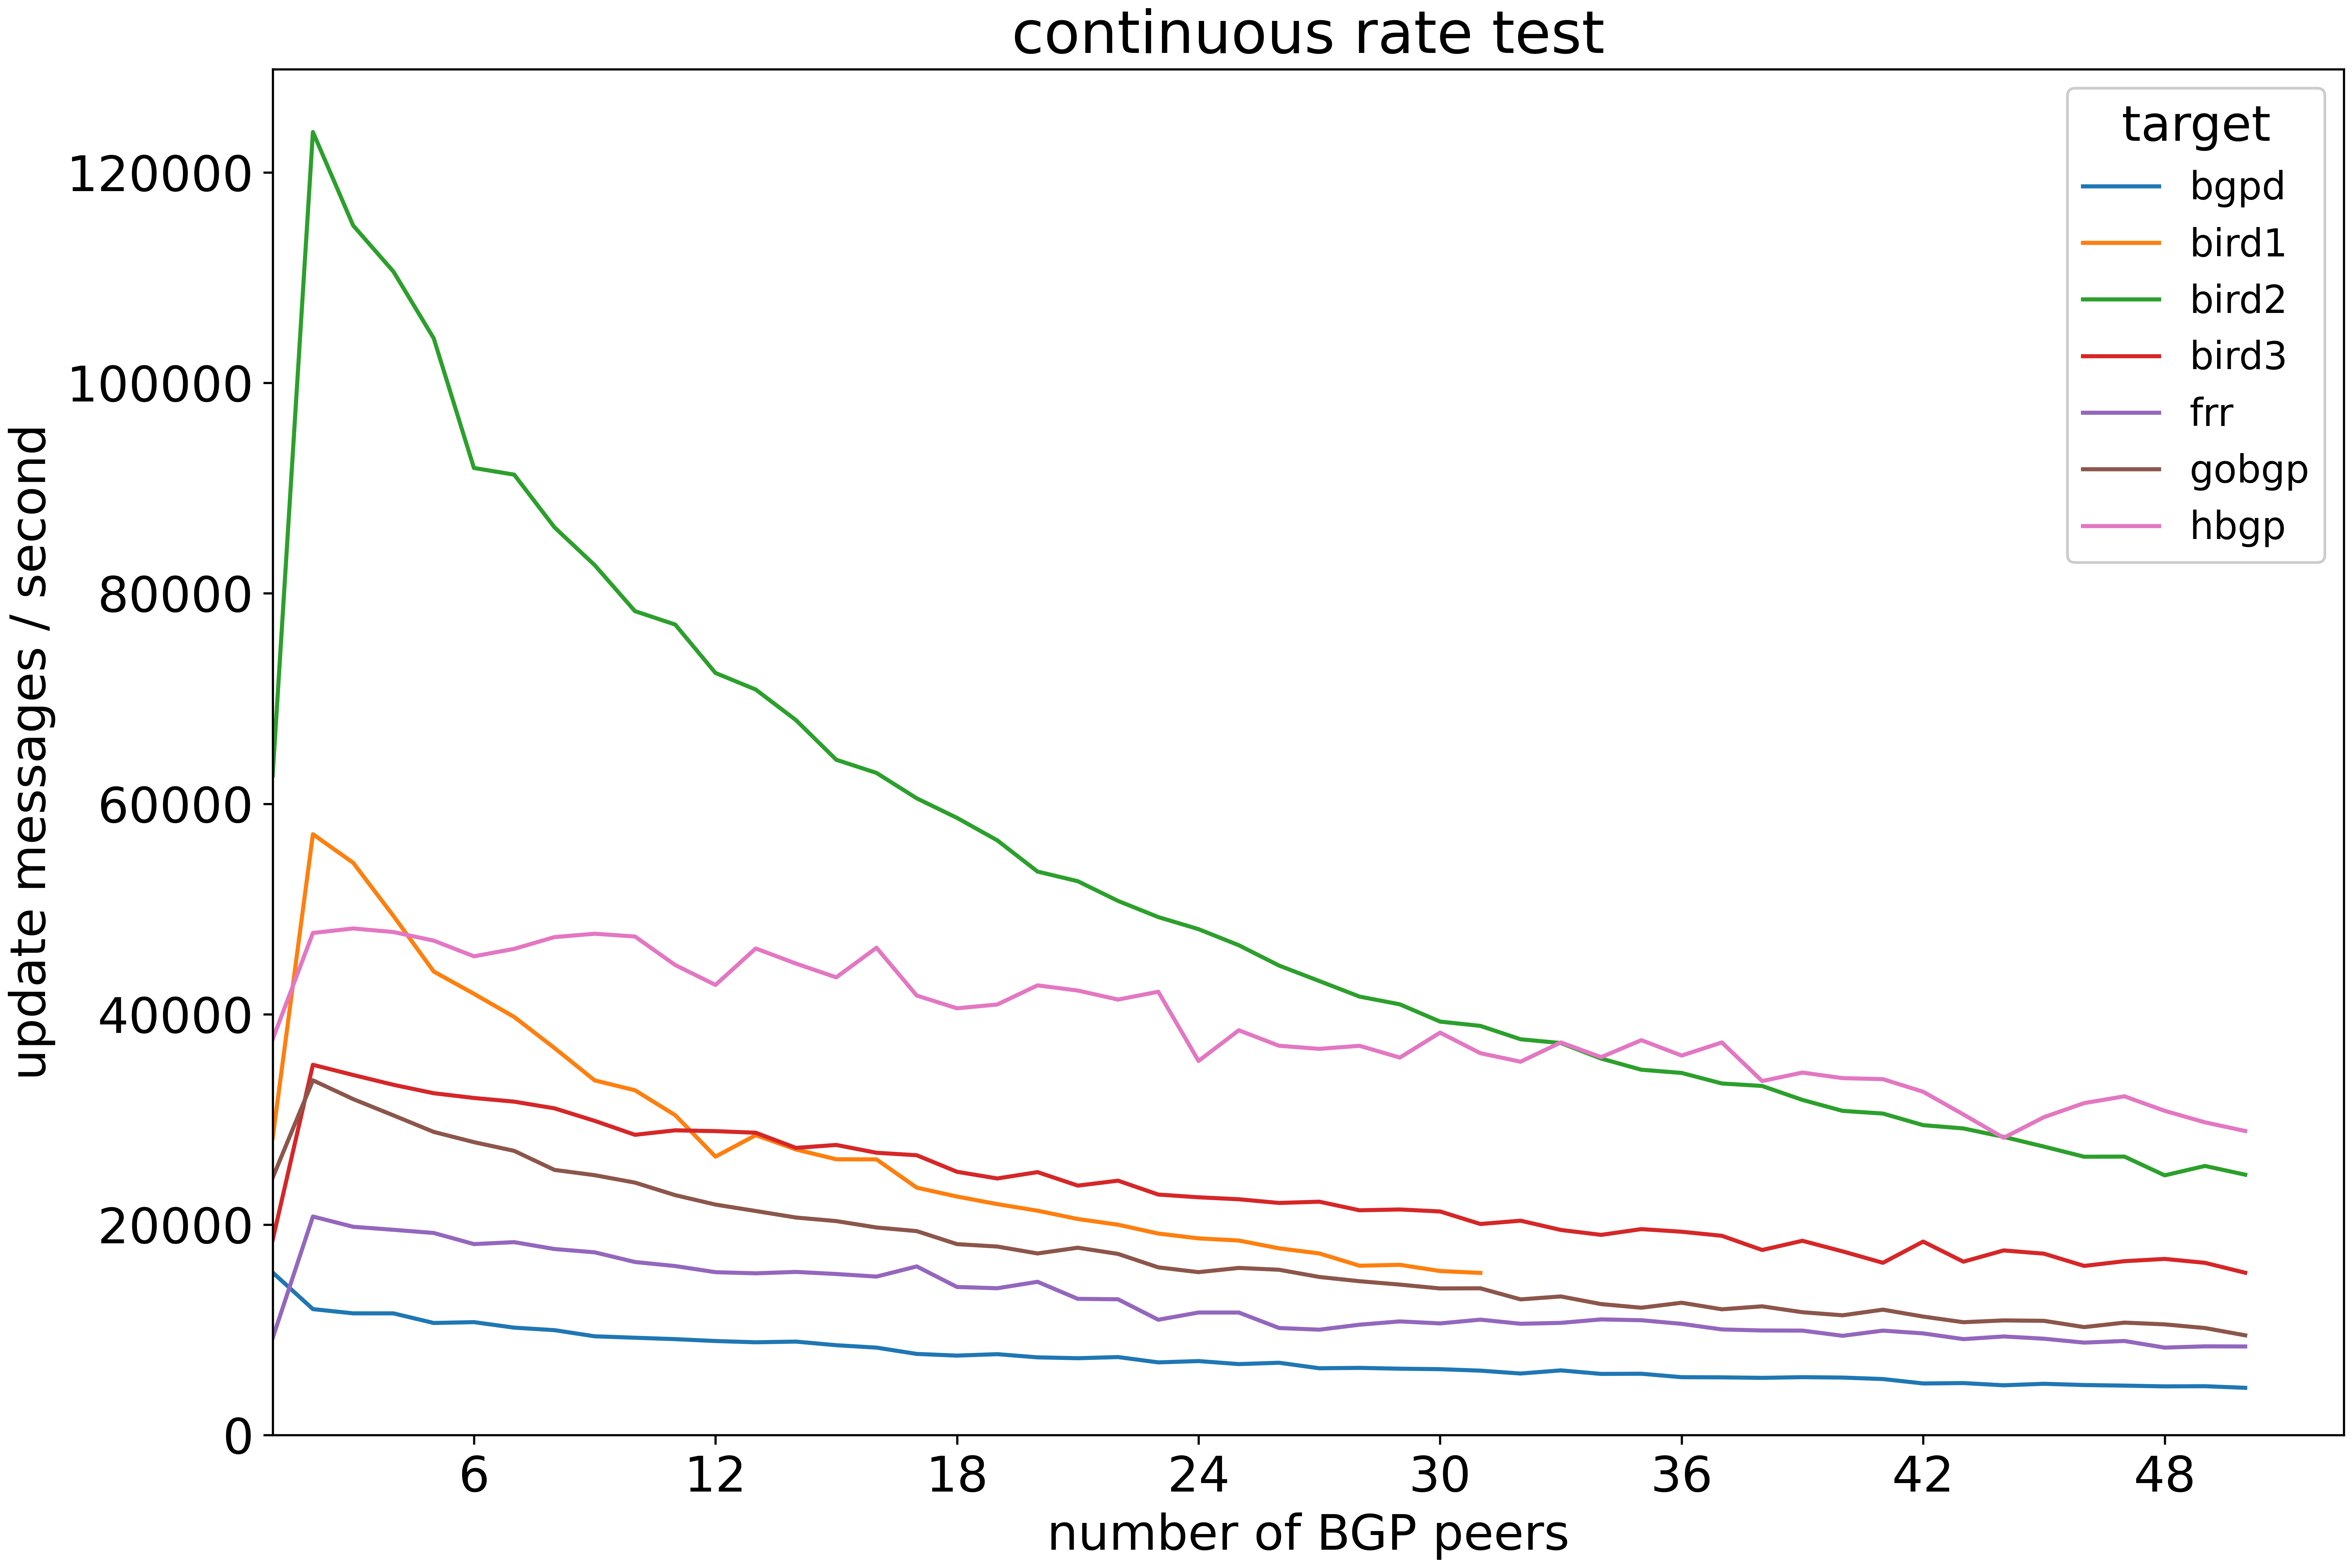
\includegraphics[width=0.7\linewidth]{1750175110.png}
    \caption{sample figure from report tool    }
    \label{fig:1750175110}
\end{figure}


\subsection{Baseline Performance: Single-Session Scenarios}
In order to establish a set of baseline measurement profiles, in this section we focus our performance analysis on the single session scenario using the metrics discussed in the previous section.
Our measurement results are presented in Table \NH{XXX?}, reporting the mean and the standard deviation of each measurement across 50 runs.
In order to demonstrate the low measurement overhead of our platform, the table reports additionally the performance measurements of our custom BGP relay implementation.
The relay BGP speaker completes the table transfer in less than 90msec, while the processing of the route updates complete in approx.
30 msec.
This measurements suggest that the impact of our measurement in the overall latency measurement is less than 10\%.
In parallel, our system generates 4x more updates than the BIRD2 speaker can process, the fastest BGP speaker in this measurement.
Furthermore, our measurement highlight that there is a significant latency difference between a table transfer and a route update for most speakers.
This can be attributed to the significant number of memory allocations that the speaker needs to perform in order to create the required state for each new route.
In terms of performance, we highlight that BIRD2 achieves the best performance across all metrics.
In addition, BIRD2 exhibits a non-negligible performance improvement in comparison to BIRD.
Specifically, BIRD2 processes 100 msec faster on average the table transfer and the route update and its average processing rate is improved by 15\%.
FRR is significantly slower than BIRD and BIRD2, especially for the average processing, which is 4x time slower in comparison to BIRD2.
Nonetheless, from a network manager perspective, FRR supports series of configuration options, not available in BIRD.
OpenBGPD performance is measured to be somewhere between the two systems.
Finally, GoBGP exhibits the worst performance in comparison to the rest of the BGP speakers.
During our measurements, we note that the GoBGP process was saturating 6 CPU cores, which suggests that the speaker was using effectively its multi-thread capabilities.
The measurement results suggest that the use of a high-level language (Go) can have an impact on the performance of a BGP speaker, due to features like automated garbage collection, while enabling multi-thread support in a BGP speaker is not guaranteed to improve overall performance.

% Original heading: \subsection{Multi-session performance}
\subsection{Scalability Analysis: Multi-Session Performance}
In order to perform this measurement, we use the ability of kakapo to establish multiple sessions towards a speaker and measure the average processing latency of a table transfer (Figure~\ref{fig:tbl-transfer-scalability}) and a 50k route update batch (Figure~\ref{fig:ssbt-scalability}) for a varying number of active BGP sessions.
Furthermore, we extend our rate estimation experiment and consider two new scenarios: the route updates are sent over a single session (Figure~\ref{fig:ssrt-scalability}) or the route updates are sent in parallel from all sessions (Figure~\ref{fig:msrt-scalability})~\footnote{In this measurement, we omit GoBGP from Figure~\ref{fig:tbl-transfer-scalability}, because the latency was extremely high and present results for up to 10 active sessions in all other figures, since the speaker kept resetting BGP session for higher session numbers}.

\begin{minipage}[c]{.49\linewidth}
	\centering
	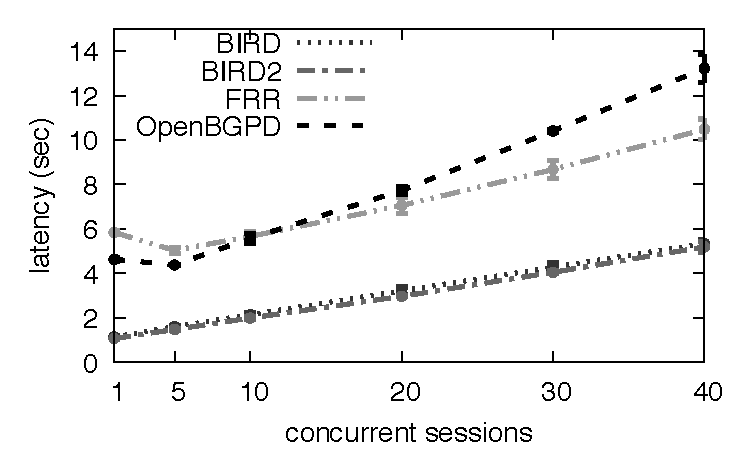
\includegraphics[width=\linewidth]{images/table-transfer-scalability.pdf}
	\captionof{figure}{Table transfer latency (800k).}\label{fig:tbl-transfer-scalability}
\end{minipage}
\begin{minipage}[c]{.49\linewidth}
	\centering
	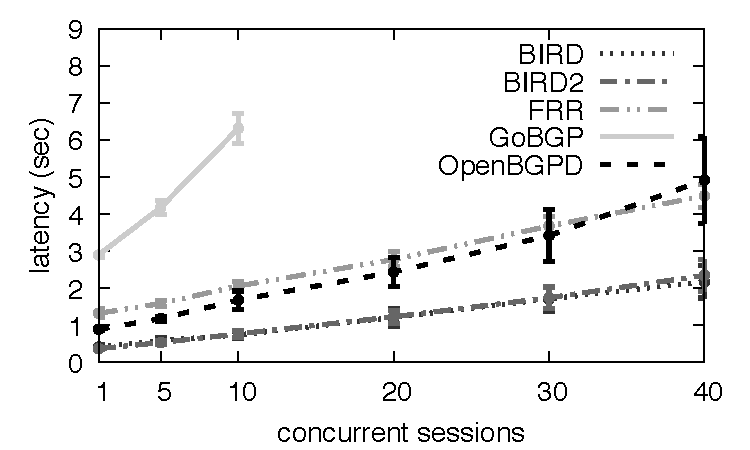
\includegraphics[width=\linewidth]{images/ssbt-scalability.pdf}
	\captionof{figure}{Route update latency (50k). } \label{fig:ssbt-scalability}
\end{minipage}
\hfill
\begin{minipage}[c]{.49\linewidth}
	\centering
	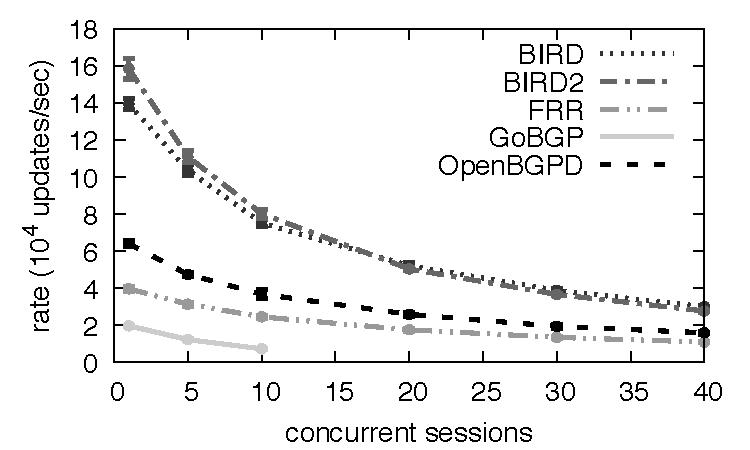
\includegraphics[width=\linewidth]{images/ssrt-scalability.pdf}
	\captionof{figure}{Single-session burst rate.}\label{fig:ssrt-scalability}
\end{minipage}
\begin{minipage}[c]{.49\linewidth}
	\centering
	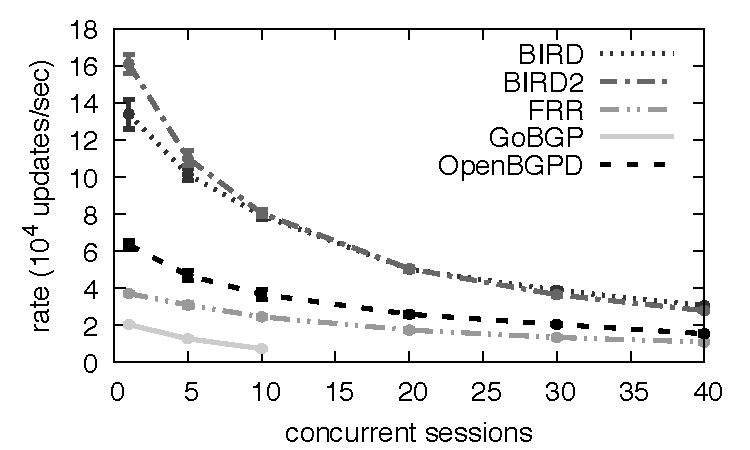
\includegraphics[width=\linewidth]{images/msrt-scalability.pdf}
	\captionof{figure}{Multi-session burst rate.} \label{fig:msrt-scalability}
\end{minipage}
\vspace{1em}

\paragraph{\textbf{Analysis}}
Firstly, we highlight that all speakers exhibit a very significant performance reduction as the number of active sessions increases.
This behaviour is consistent in table transfer, update burst and continuous rate measurement scenarios.
BIRD and BIRD2 appear to experience a significant processing rate reduction for high sessions numbers, since their processing rate halves as we increase the number of sessions from 1 to 10.
Nonetheless, this performance impact is not similar in the latency measurement, and both speakers exhibit a sublinear performance decrease.
OpenBGPD and FRR exhibit a sublinear decrease in their performance for both latency and rate measurements.
These characteristics might be explained either by the employed lookup structures, which increases its lookup times for large route counts, or the internal processing scheduling mechanism.
Secondly, for all BGP speakers, BGP performance varies only slightly when route updates are spread across multiple sessions.
Across all speakers, there a minor performance decrease on the order of 1\%-2\% on the average route processing rate.
This highlights that while all systems manage gracefully large update bursts coming from multiple parallel sessions, such as may occur during major route instabilities, however none of them manage to leverage the opportunity for parallelisation to actually improve performance.

\subsection{Impact of Transmit Window Size in Continuous Mode}
First we show as an example the results of a simple test case in which three different versions of the same open-source BGP speaker are deployed.
\ref{fig:rw_fig1}

\begin{figure}[H]
    \centering
    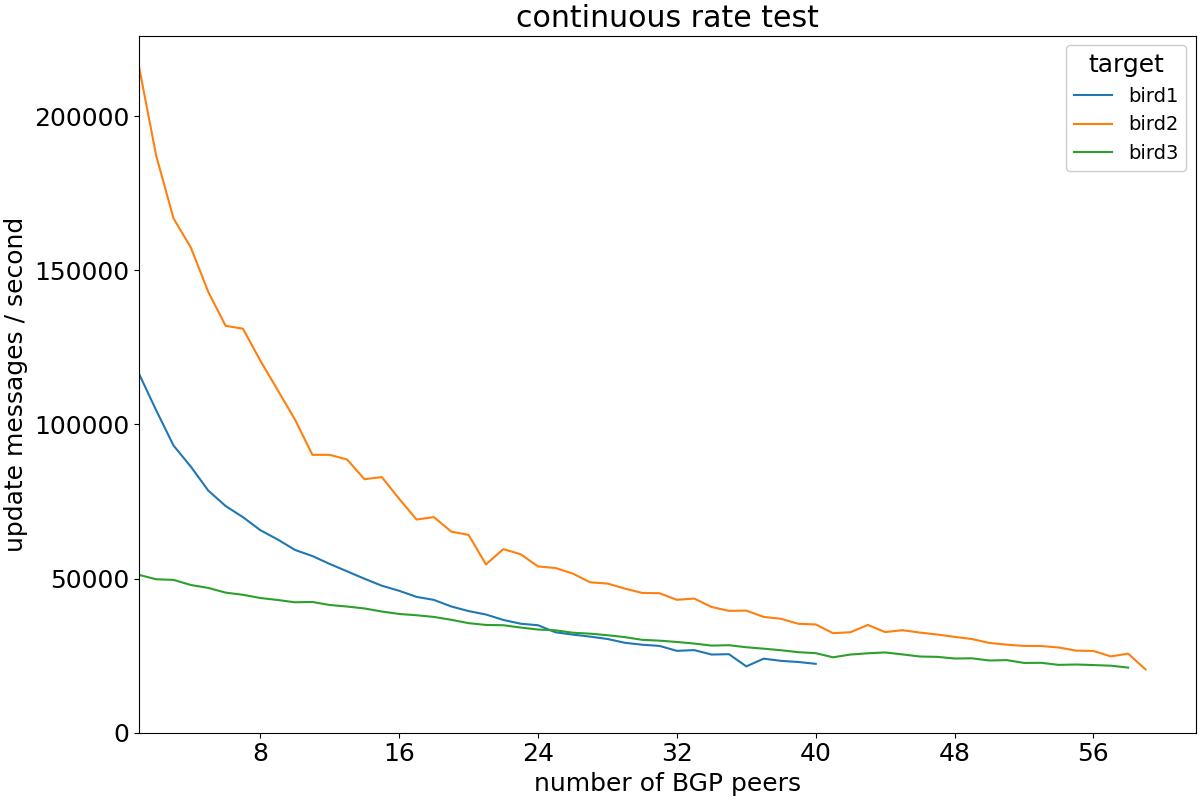
\includegraphics[width=0.7\linewidth]{ratewindow/Figure_1.png}
    \caption{rate test over varying number of source peers}
    \label{fig:rw_fig1}
\end{figure}

In the second version of the same graph the test results include the reference BGP implementation ‘relay’, which provides a benchmark measurement to give some confidence that even for the best performing BGP implementations, the measurement framework itself is not a significant drag on observed performance.
\ref{fig:rw_fig1a}

\begin{figure}[H]
    \centering
    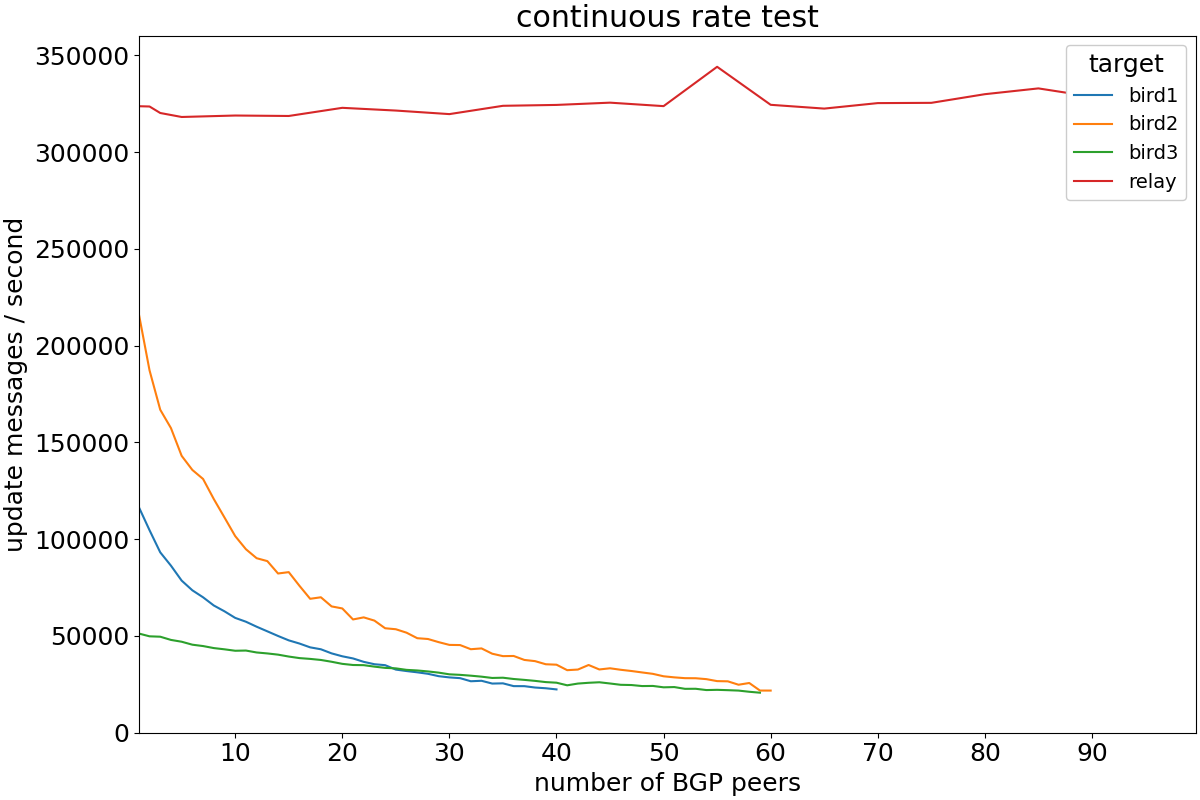
\includegraphics[width=0.7\linewidth]{ratewindow/Figure_1a.png}
    \caption{rate test over varying number of source peers - with `relay' baseline}
    \label{fig:rw_fig1a}
\end{figure}

In these next graphs, the impact of the chosen window size is evaluated.
We hypothesise that for any given BGP speaker there should be some optimal value of window size, a value which is relatively small compared to the full table size bursts applied in Kakapo block mode.
We can also expect that, for very small windows sizes, the lower rates achieved may ultimately be limited by processing latency in the BGP speaker, which can be seen as a distinct measure to `performance under sustained load', but is nonetheless an independent and meaningful performance metric.

\begin{figure}[H]
    \centering
    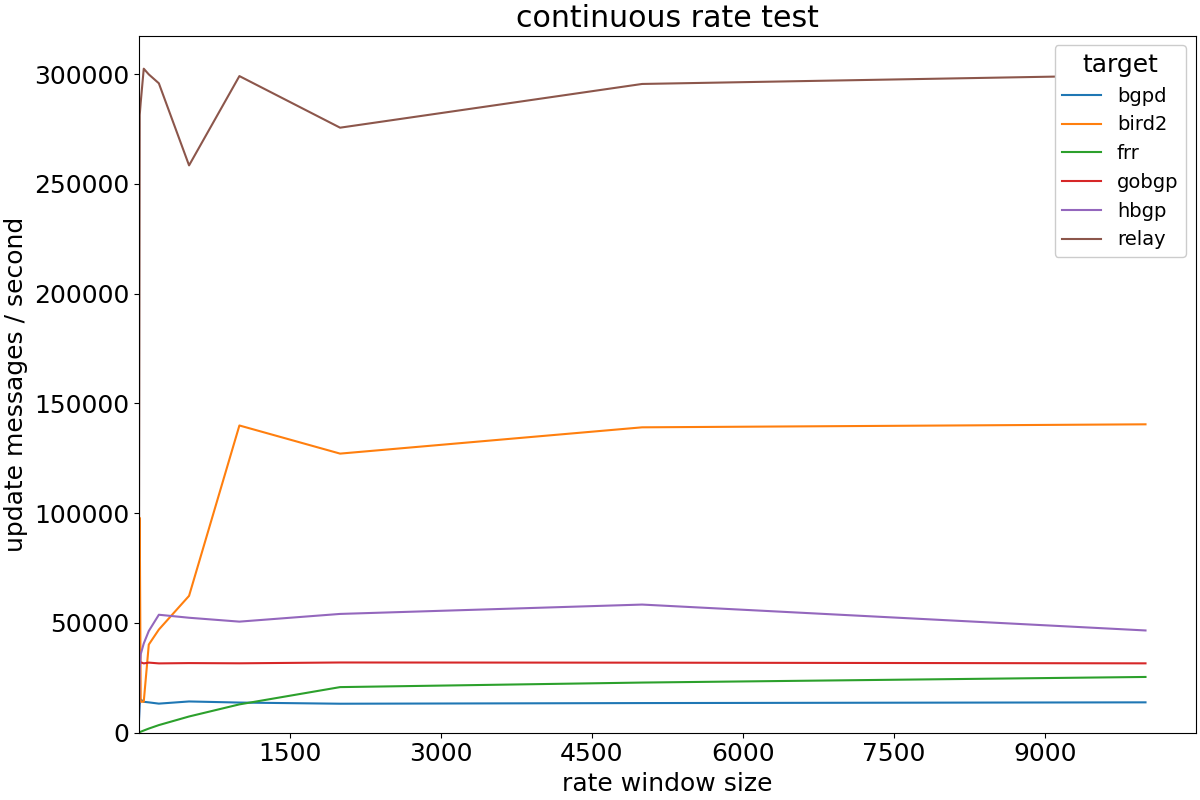
\includegraphics[width=0.7\linewidth]{ratewindow/Figure_3.png}
    \caption{rate test - fixed peer count, adjusting the rate transmit window }
    \label{fig:rw_fig3}
\end{figure}

\paragraph{analysis of \ref{fig:rw_fig3}}
Absent some interesting anomalies around the smaller window sizes it can be seen that above a transmit window size of 2000 messages, all BGP speakers approach some reasonable level of consistency for throughput.

There are some  anomalies, the most obvious and distinct is the behaviour of FRR \- for very small window sizes, FRR does much worse than any other BGP speaker.
This is quite easily explained by the observation that FRR is the only BGP implementation tested which universally applies the default Linux TCP DELAY (Nagle algorithm).
The newly implemented BGP endpoints all set the Linux socket option TCP\_NODELAY, and it is safe to assume that the others, apart from FRR, do the same.

Another anomaly arises in the case of bird2, better seen in this expanded version of the figure, limited to smaller windows sizes:

\begin{figure}[H]
    \centering
    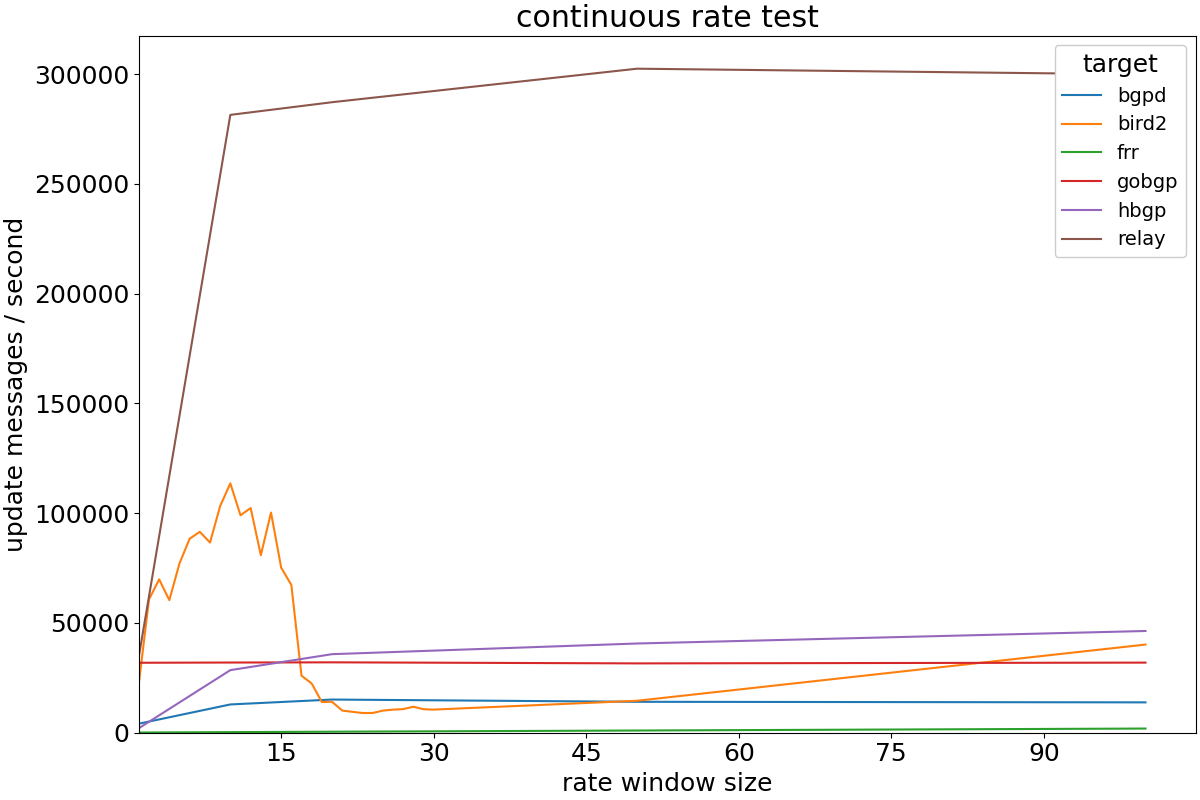
\includegraphics[width=0.7\linewidth]{ratewindow/Figure_3a.png}
    \caption{focus on bird2 sensitivity to small transmit window sizes }
    \label{fig:rw_fig3a}
\end{figure}

Here it can be seen that there is a real and repeatable anomaly in the case of bird2,for window sizes less than 20.
There is no obvious explanation for this effect.
This graph also illustrates significant differences between each of the other BGP speakers: since the performance in this realm is effectively a measure of latency, the measurements are not entirely trivial, and the merit ranking is strikingly different from others in this study:
\begin{itemize}
     \item For window sizes below 15, bird2 is ‘better’, followed by gobgp: gobgp is strikingly consistent, to such an extent that it could be worthy of investigation in its right.
     \item Then, in the realm of windows sizes from 15 to 100, consistent trends are established that extend up to the larger windows sizes of the main graph, the exceptions being FRR, for which a window size of 2,000 are greater is needed in order to achieve the best throughput of which it is capable, and bird2, whose actual and relative performance falls from best to 4th of 5\.
     \item At window sizes above 100 bird2 starts to reemerge as a much higher performer than the rest of the group, although it is still less capable than hbgp until the window size reaches 250.
     \item Bird2 reaches its best throughput of around 140k updates/sec at a window size of 1000; the next best BGP speaker, hbgp, achieves around 50k updates/sec in this scenario.
\end{itemize}

Note however that this test runs only a single source update peer: when a larger number of source peers is configured, bird2 performance degrades and eventually is overtaken by hbgp.

\begin{figure}[H]
    \centering
    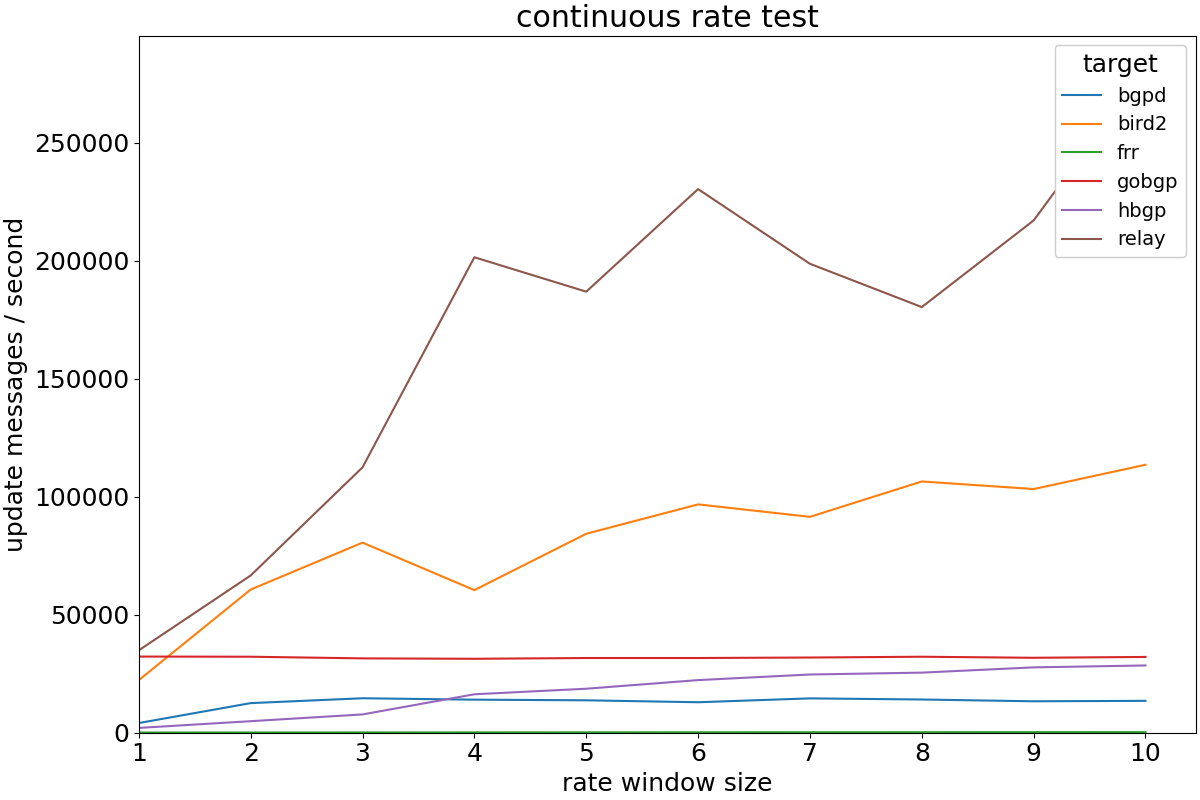
\includegraphics[width=0.7\linewidth]{ratewindow/Figure_3b.png}
    \caption{TBC }
    \label{fig:rw_fig3b}
\end{figure}

The final word should be said on the baseline measurements using the reference null bgp implementation, ‘relay’.
This greatly expanded view of the same rate data (\ref{fig:rw_fig3b}), achieved with the smallest, single digit, windows sizes, shows that until the window size reaches 4, the performance of bird2 is only slightly below the reference implementation, so that for this case it would be wise not to attach to much significance to the exact values reported.
However, since the gap between reference and bird2 widens and remains consistently wide for larger window sizes, it seems unlikely that the experiment ‘unfairly’ negatively represents the capability of bird2.
For higher confidence  insight,  the best technique would be to analyse packet trace data with accurate timestamps, in order to measure latency directly.
Since latency performance is not a major focus of the work, the refinement of the kakapo tool for precision latency measurement is left for future work.
This figure also serves to further underline the remarkable consistency of the metric for the gobgp case.

\subsection{Impact of Prefix Packing on Processing Performance}
The BGP message protocol supports a convenient and universally applied optimisation, which is to allow routes with common path-attributes to be advertised in a single Update message.
Other than as an optimisation, there is no semantic distinction between a single Update carrying \textit{N} routes, and \textit{N} Update messages, each carrying a single route, if the path-attributes otherwise remain identical.
Here, the practice of combining routes in this way is referred to as prefix packing.
The subject of investigation is how the usage, or otherwise, of `prefix packing' affect the performance of BGP speakers.
It is a worthwhile question, not least because the requirement to maintain packing structures on BGP Update flows presents a very serious challenge for designers of BGP systems, and especially for designs intent on parallelising processing as far as possible.
Were an otherwise `credible' new BGP system to be proposed, but one which often or always did not optimally pack routes in Update messages, it might be hard to gain acceptance for real-world applications.

\subsubsection*{Experimental Approach}
In these investigations the existing Kakapo measurement tool is deployed, applying a procedural variation to force all transmitted messages to be `unpacked'.
Kakapo supports this behaviour with a parameter `NOPACK', which is either globally enabled, or not (the default).
The measurement set reported is a repetition of the canonical, single peer, continuous, rate test, already described.
All of the standard BGP implementations are evaluated under NOPACK operation, as is hBGP \footnote{the baseline test tool relay is not reported - there exists some defect in the tool which prevents reliable completion of test runs.
It is the only known deficiency in relay, to-date.}

\subsubsection*{Experimental Results}
The table \ref{tab:packing} shows summary results, for sustained processing rate, and also for initial route table load (`conditioning').
With a single remarkable exception, all tested BGP speakers exhibit some degree of impact of unpacked operation.

\begin{table}[htbp]
\centering
`
\begin{tabular}{ccccc}
\toprule
\thead{BGP Speaker} & \thead{Rate \\ Packed Updates} & \thead{Rate \\ Unpacked Updates} & \thead{Percentage \\ Reduction} & \thead{ Reduction \\  Ratio} \\ \midrule
bgpd  & 13266          & 57683            & 435\%             &      
            \\
bird1 & 61384          & 45062            & 73\%              & 1.36            \\
bird2 & 131958         & 90549            & 69\%           
    & 1.46            \\
bird3 & 35521          & 29575            & 83\%              & 1.20            \\
frr   & 21642          & 14503            & 67\%   
            & 1.49            \\
gobgp & 33201          & 5297             & 16\%              & 6.27            \\
hbgp  & 42910          & 13192        
     & 31\%              & 3.25            \\ \midrule
vMX	& 4833		& 4461		& 92\%		& 1.08          \\
`
vIOS		& 2053		& 565		& 28\%		& 3.63           \\ \bottomrule
\end{tabular}
\caption{Comparative performance (Update processing rate - routes per second ) of BGP Speakers, when Update Prefix packing is disabled on the input stream}
\label{tab:packing}
\end{table}

\subsubsection*{Analysis}
The mainstream BGPs, BIRDx and FRR, handle the unpacked input with reasonable grace, the same time `fixing up` the suboptimal format for downstream peers, as does Juniper vMX.
Given that the raw message rate is a factor of 10 greater, a performance decline of 10\% to 30\% is not unreasonable.
The outliers are the BGP newcomers - gobgp suffers the most - a factor of greater than x6, and \hbgp by more than x3 - even though neither of them are able to re-aggregate the resulting Update stream.
Interestingly, the Cisco virtual router also performs poorly - performance drops by more than a factor of 3.
However, Cisco and the Juniper vRouters do at least re-aggregate the Updates on re-announcement.
An additional observation can be made, which is whether the BGP speaker under test packs prefixes when re-announcing them.
This observation is carried out by taking sample packet traces and analysing with Wireshark \footnote{This sample based analysis does not prove that the identified behaviour is uniformly applied, but it seems reasonable to assume that a mid-stream analysis of several updates in sequence is representative.
However, caution is wise on the assumption of consistent behaviour: it is known that early versions of FRR were prone, under stress, to not packing Updates received as packed.}
The observed behaviour is that for bird and FRR only \footnote{and also the Cisco and Juniper vRouters}, Updates are consistently packed.
No other implementation packed Updates, when those received, were not themselves packed.
OpenBGP/bgpd is perhaps the most surprising case, for two reasons - which may be related: OpenBGP is the only BGP implementation which actually runs faster in unpacked mode, in the continuous mode test, and, of all of the `mature'  BGPs, it is the only one which does not actively repack arriving unpacked Updates.

\subsection{Influence of the Execution Environment}
In this next graph the impact of test context is shown \- the same set of measurements is taken using a laptop execution environment, varying the power control settings between ‘performance’ and ‘power saving’.

\begin{figure}[H]
    \centering
    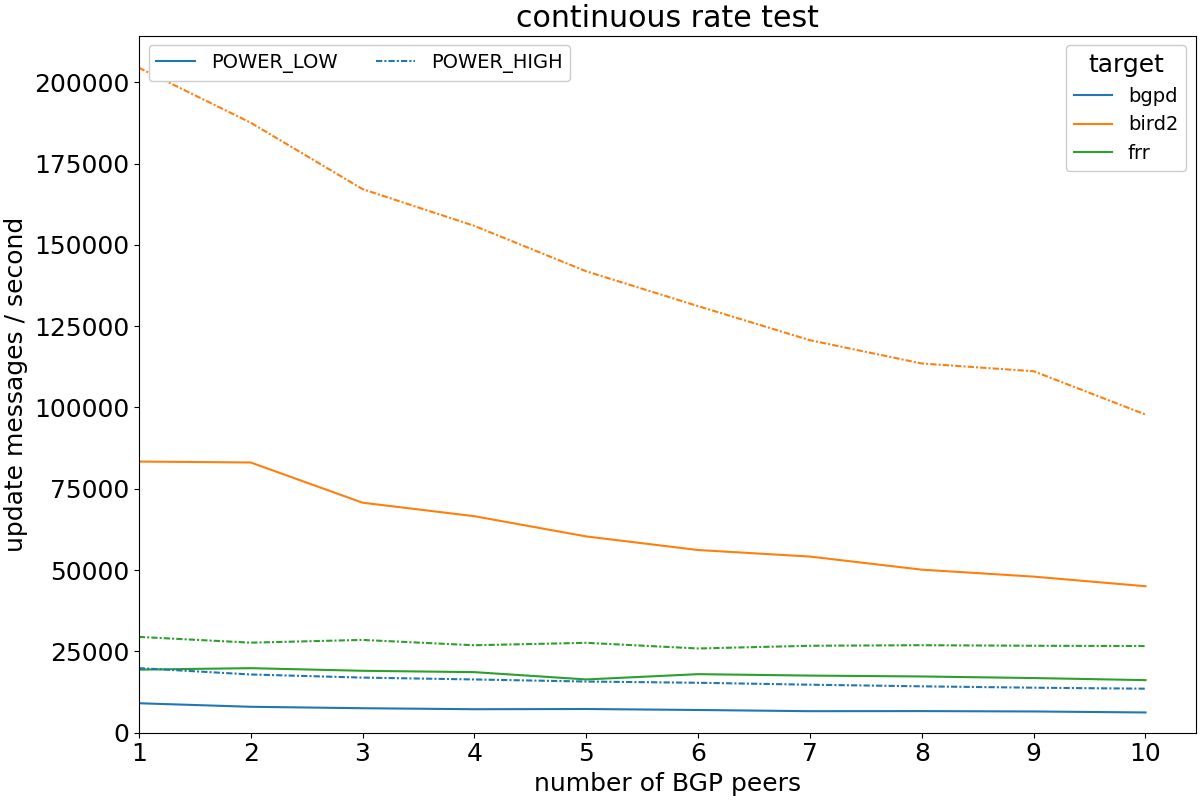
\includegraphics[width=0.7\linewidth]{ratewindow/Figure_2.png}
    \caption{TBC - fig 2}
    \label{fig:rw_fig2}
\end{figure}

Unsurprisingly, the performance changes, but it is noteworthy that the effect is not entirely linear.
For bird2, the low and high power performance ratio is between 2.2 and 2.5, whilst for frr the ratio is only between 1.5 and 1.6.
No examples are known where execution context changed actual relative ordering of targets, but it illustrates that careful curation of execution parameters is essential, and statements such as ‘BGP-x is 5x faster than BGP-y’ should be treated with great caution, even when the specific test and scale are made explicit.
The next graphs illustrate such pitfalls in more detail.
The first is the above graph, but with additional power contexts, of which one is running on another hardware platform \- a rack server with high memory and CPU count, while evidently less performance on a single CPU.

\begin{figure}[H]
    \centering
    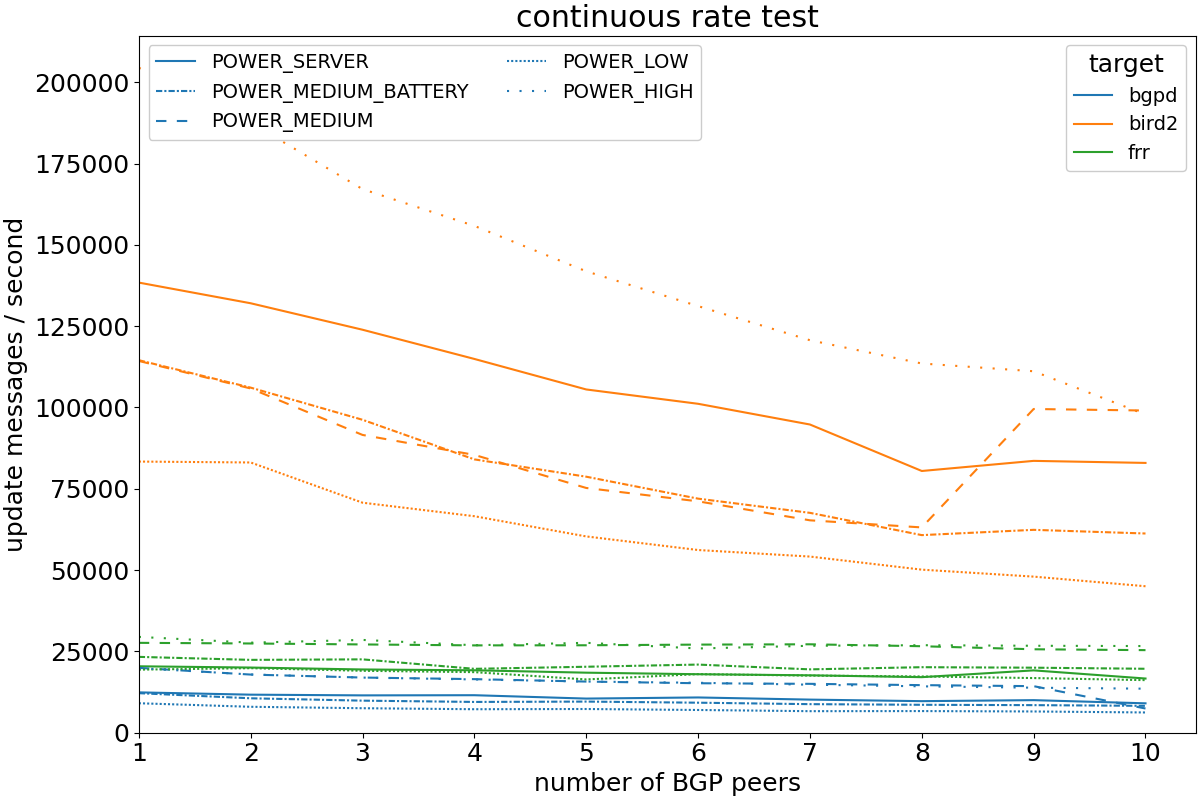
\includegraphics[width=0.7\linewidth]{ratewindow/Figure_2a.png}
    \caption{TBC - 2a}
    \label{fig:rw_fig2a}
\end{figure}

The especial factor here, other than that a laptop may often beat a high spec server when single or low core count applications are concerned, is that for the laptop, running on battery risks producing highly unreliable outcomes.
To safeguard against this source of inconsistency the kakapo framework records power supply status and when graphing experimental data records which show BATTERY as power source should be discarded.
And of course, for comparative purposes data from different hardware platforms should rarely be processed in the same analysis.
The above graph is the only case in which data from two hardware platforms has been combined for any reported experiments.
One more interesting observation selected from the same dataset:

\begin{figure}[H]
    \centering
    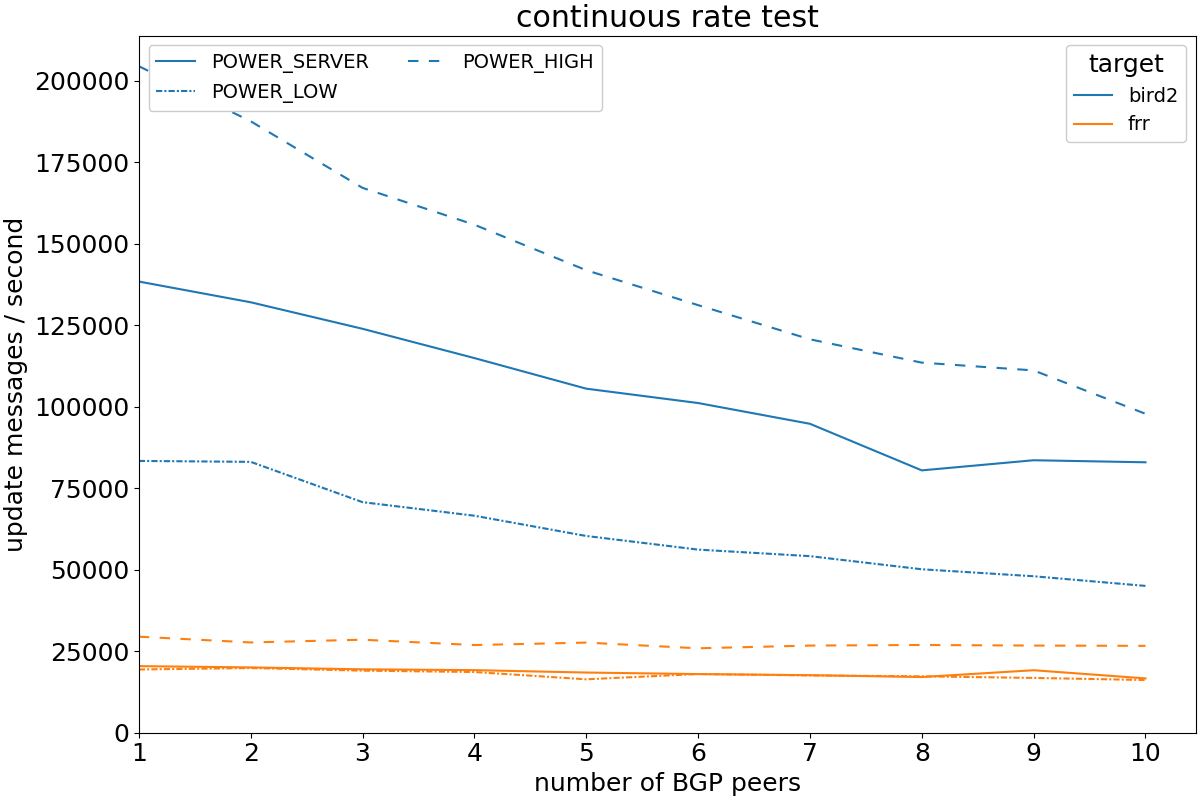
\includegraphics[width=0.7\linewidth]{ratewindow/Figure_2b.png}
    \caption{TBC - 2b}
    \label{fig:rw_fig2b}
\end{figure}

Here, the remarkable observation is that, for the frr workload, the laptop ‘power-saving’ performance is approximately the same as the server, yet for bird2 workload the server is as close to laptop ‘performance’ mode as to ‘power-saving’ mode.

\section{Conclusions}

kakapo has enabled the qualification of performance and stability of the new and novel BGP implementation, \hbgp.  In doing so, it has also provided significant insights into
\begin{myitemize}
    \item the challenges of evaluating BGP speaker performance
    \item the variability and performance envelope of well some known BGP implementations
    \item significant, and in some cases serious, shortcomings, at least as regards use for core IDR, in some of the platforms investigated.
    \item cautionary experience for those undertaking BGP performance evaluations, based on simpler methodologies
\end{myitemize}

In particular, the development and application of the continuous mode testing capability shone surprising light on several BGP implementations, as did the work exploring larger number of concurrent peer sessions.

The discovery that the `gold standard' for BGP performance - bird2 - is not always as distinctive as initial work seems to show was interesting, as was the discovery that the latest version of bird - bird3 - is significantly slower than its sibling/ancestor, bird2.

The initial, and most important, aspect of the work with kakapo was to provide validation that the new BGP platform built for the wider project was, as far as can be measured, comparable and, in many cases, even faster than existing well known BGP implementations.
Whilst \textit{very} early versions of Haskell BGP were not as performant - in particular, the initial experiments using Software Transactional Memory (STM) \cite{GHC-STM} \cite{STM2005}.

However, the most important role of kakapo in the development of \hbgp was as a stress and soak-test tool, although even here, the experience of building and improving performance for BGP in Haskell was surprisingly painless; probably the more testing procedures were functional tests, which required interoperability with the range of BGP speakers available, and in various roles and topologies.

\bigskip

Perhaps the most important validations of all are  

\begin{enumerate}
    \item The viability and practicality of  Haskell  \hbgp, in its controller variant form, for use at IDR scale - showing that it is possible to introduce external programmability to a `normal' BGP speaker, albeit one written in Haskell, without significant impact on its ability to perform, at scale, and at speed.
    \item The viability of applying a very high level Functional Programming language in a new and highly challenging domain - it is can be asserted that it is possible to build safer, more reliable and more flexible network protocol systems than could ever be achievable in `C', given the well known limitations of the `C' language, and the current trend to replace `C' in mission critical applications, with safer alternates.  The proven productivity gains of using Haskell only serve to reinforce the point, that future network systems can, and surely will, no longer be written in `C'.
\end{enumerate}

\section{kagu}


\subsubsection*{ kagu framework architecture}

kagu uses  both containers (Docker) and virtual machines (libvirt/kvm/qemu).  Libvirt is used to create long-lived topologies whose members are test agents, test targets and the virtual network links which integrate the distinct VMs into a single connected system.  The motivation for this high level design is to provide a controlled and configurable execution environment for virtual routers and test agents.  The system is designed to enable moderately large networks containing interlinked multiple test targets and test agents, such as is required to validate system level behaviour in multi-AS BGP networks.  Hardware virtualisation is required because the representative commercial grade BGP systems are provided as VM images, and are not based on Linux operating system. `
 `
 % One of the kagu subsystems is responsible for building these topologies, including the automatic generation of mesh topologies, and another kagu component, a guest VM agent, enables auto discovery of virtual neighbour addresses and interfaces without explicit, per guest node, configuration.  This is otherwise non-trivial when all the inter-VM links are point to point, so that no system level address autoconfiguration scheme (e.g. DHCP) is available, and in fact in data centre BGP implementations there are extensions to BGP to support just these capabilities.  Unfortunately, these extensions are not applicable to this test environment, and are not supported in the software of most of the BGP systems in the list of targets.  `
Whilst this design achieved the goal of delivering a suitable hardware infrastructure it complicates the test orchestration task, even without considering the issues of exception management.  In the initial kagu design the approach adopted was to use remote ssh shells to monitor and execute every aspect of the tests, however this proved to be both unreliable and extremely complex to build.  The eventual solution is simpler, more reliable and more capable and flexible \- the solution adopted is ‘remote docker’.  This approach builds a single standardised VM container which can be used for all test targets, test agents, and all distinct nodes in a test constellation. Nodes are configured by role using different docker images, and configured for node specific identity by configuration files injected into docker instances.  Finally, the problem of collecting exception context is solved by a combination of Docker’s  internal logging via systemd/journald, and the innovation of defining core-dump destinations as files mounted *outside* the docker container.  In this way, each Docker instance can be managed as a single logical object which may be stopped on command, or exit unexpectedly, with error status, yet whose exception logs are reliably persisted in a central location, independent of the execution environment.  The critical capability provided by Docker is the facility to control *and log* Docker daemons on remote servers from a remote single separate control node. `

Implementation note: in all cases Docker instances are run in a privileged mode in the host VM, in order to allow the running BGP speaker to have direct access to all network interfaces; the reason that Docker alone is not sufficient itself for this application is that although Docker can be used to restrict guest processor and memory allocation it was not found possible to manage the virtualised network topology using Docker in the way that is possible with libvirt/kvm, and secondly, some test target are not available for native Docker use since they are provided as KVM VMs.

% #### ‘testscripts’

% ‘testscripts’ refers to the interactive, tmux based, alternative to ‘kagu’.  Functional test don’t require repeated lengthy execution, but they do require immediate in depth visbility of routing response after different stimuli.

% #### testscript deployment and uses cases

% # Bootstrapping a test environment: full instructions

% The target environment is a current Linux distribution system capable of running qemu/kvm virtualised hosts.  A medium-spec laptop or desktop is required \- the limiting factor is RAM and virtualisation capable CPU \- an 8GB machine has been used successfully.
\NH{need to pull in here the BGP protection test setup}

% \section{PIR test implementation guide}

\NH{\rule{14cm}{0.4pt}}

\NH{this text is to be relocated in the kagu section}


\subsection{functional components of PIR test environment}

\subsubsection{server, OS, virtualisation host}

The current server and OS are Ubuntu Linux 22.04 (laptop) and Ubuntu Linux 20.04 (rack mount server).
Laptop has 32 GB RAM and 14 CPU cores (Intel i7-1280P), server 128GB RAM, 20 CPU cores (Intel Xeon D-1747NTE).

Virtualisation support is standard Linux KVM/qemu managed with libvirt.
Container technology is standard Docker.

\subsection{virtual routers, software routers}
\subsubsection{versions}

\begin{enumerate}
\item Cisco virtual router: IOSv - VIOS-ADVENTERPRISEK9-M - Version 15.7(3)M3
\item Juniper virtual router: Junos VMX - JUNOS 18.2R1.9
\item Bird.cz - BIRD2 - version 2.15.1
\item frr - version 8.4.4 (installed via package manager in ubuntu24.04)
\item OpenBGPD - version 8.6
\item gobgp - version 3.35.0
\end{enumerate}

\subsubsection{build procedures - Docker images}

\begin{enumerate}
\item Bird2 and OpenBGPD are built from source
\item frr is installed as an ubuntu package
\item gobgp is installed as a binary from OSRGs github repository.
\end{enumerate}

\subsubsection{build procedures - virtual router images}

\begin{enumerate}
\item <reference source file directory>
\end{enumerate}

A custom configuration tool was developed for both Cisco and Juniper as an 'expect' script which drivers a clean router instance by invoking command line scripts which copy in the configuration files based on the router role requested.  The configuration files consist of 'standard' IOS and Junos configuration CLI commands.
The scripts allow many full router configurations to be maintained and updated and used on demand to (re-)create the desired set of routers for an experiment.

A virtual router is built from a suitable 'qcow2' image using the 'virt-install' tool and nominating the OS variant as freebsd12.0'.

Junos images are assigned 4Gb RAM and use 'virtio' network drivers.

Cisco images are assigned 2Gb RAM and use 'e1000' network drivers.

The virtual image builder is developed under the project heading 'kagu'.


\NH{\rule{14cm}{0.4pt}}

\section{`Smoketest'}

\subsection*{What is smoketest?}
'smoketest' is the core test \textit{framework} (\textit{kakapo} is the core test BGP speaker).

\begin{figure}[H]
    \centering
    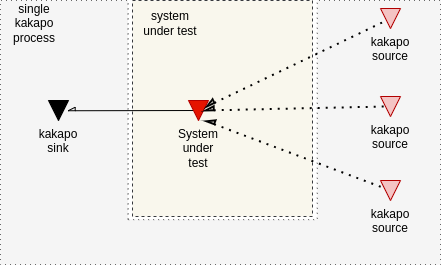
\includegraphics[width=0.7\linewidth]{images/bgp6.drawio.png}
    \caption{standard kakapo test deployment configuration}
    \label{fig:diag6}
\end{figure}

It orchestrates concurrent instances of a wide range of target test BGP systems and the BGP test system, `kakapo'.

In general, most of the test BGP systems are run under the control of Docker\footnote{Cisco vIOS and Juniper vMX are run as full virtual machines under KVM}.

The test procedures orchestrated by smoketest are all variants on a `standard' kakapo configuration\footnote{The following description is best understood after reading about kakapo in the previous section.}, i.e., kakapo emulates two or more BGP endpoints to act as BGP route sources of sinks, all of which are configured as direct peers to the single System-Under-Test.
Kakapo route-source endpoints announce new routes according to some pre-defined pattern, and a singleton kakapo route-sink monitors the relayed routes as they are re-announced by the System-Under-Test (SUT).


\section{kagu - alt 1}


\subsection{Kagu: BGP experiment automation}

A major challenge for network experimentation is reproducibility. Kagu is an
automation platform, built around kakapo, allowing experimenters to deploy and
parallelise the execution of BGP experiments. In parallel, kagu also automates
measurement data and logging information collection for offline processing.

OS virtualisation is a key technological enabler for Kagu, which supports
integration with docker and the libvirt management library.  The docker
integration allows kagu to run kakapo and software router as docker containers
and to use docker management operations to spawn and terminate them.
Furthermore, detailed logging information are collected through the
systemd/journald services in the container. In order to run an experiment, the
platform requires as input the router and the kakapo configuration parameters
and the platform will use docker technologies to execute the experiment and
collect the results.

Furthermore, libvirt integration allows kagu to deploy large-scale experiments
with complex network topologies over a hypervisor-based virtualisation
platform, like KVM. VMs derive from a base Ubuntu image with the dockerd
daemon installed and configured to exposes remote access via HTTP.

During the deployment of a multi-host experiment, kagu builds all the required
virtual links between VMs, as well as a control plane network which uses
dynamic DNS and cloud-init to map VM control interface addresses to user
friendly host names. A custom libvirt network topology provisions distinct
unique virtual network address blocks onto each VM and dynamically updates the
configuration of a local DNS server.  Finally, the framework offers an
arp-router agent which install routes to loopback and allows connectivity over
unnumbered network interfaces.

Both test harness (kakapo) and target systems are bundled as Docker images
which enables them to be easily started and stopped in remote virtual machines
using the ‘remote Docker’ feature.  Remote Docker allows standard Docker
commands, such as ‘docker run’, ‘docker kill’ and ‘docker pull’ to be executed
on arbitrary target systems from a single controlling machine  Thus a cluster
of multiple VMs having varying resource capability can easily be orchestrated
to run multiple sets of experiments in parallel.  A complementary set of
scripts (kakapo-virt) is used to create and provision the target virtual
machines.

The main system elements are:

\begin{itemize}
	\item kakapo core  a ‘C’ language BGP test tool which can act
	      as a BGP peer, operating simultaneously in both route sink and route source
	      modes
	\item kakapo relay  a ‘dummy’,‘C’ language, BGP router which allows
	      baseline calibration of the test system
	\item kakapo runner  a run-time
	      integration framework for controlling multiple test runs with ranges of
	      test parameters
	\item kakapo ingest  offline analysis of the test data
	      generated by kakapo, including on-demand gnuplot graph display
	\item
	      kakapo-virt  a VM and virtual network provisioning tool --- kakapo virt
	      creates and provisions test VMs with different resources (CPUs, RAM,..) to
	      provide execution environments for kakapo targets and test harness instance
	      to execute in.  Kakapo-virt also provisions both a control plane network to
	      allow remote orchestration of the VMs and their Docker execution
	      environment, and a separate experimental network context which meshed VMs
	      which are configured to operate as a single experimental topology
	      somewhat like mininet, but for KVM virtual machines.

	\item kagu a build and deploy system for the (mostly Dockerised) components of kakapo
	\item arproute a network utility which enables virtualised systems to discover routes between themselves without manual configuration.
	\item Docker, systemd, libvirt and nginx with webdav support --- provides the infrastructure environment in which kagu and kakapo operate
\end{itemize}

Of these components some work before a testing session (kagu, kakapo-virt), and
others after testing sessions have finished (kakapo ingest).  The core system
consists of kakapo core, kakapo relay, kakapo runner: of these kakapo runner
is the coordination tool: it schedules execution of test systems in virtual
environments, typically systems consisting of kakapo core paired with another
BGP speaker such as bird, frr (quagga), OpenBGP, hbgp, or another hardware or
software router.  Kakapo core starts and stops BGP peer sessions with the
SystemUnderTest, monitors the response performance and records the
configuration and results in test data files on a centralised storage system
for later analysis.  Kakapo runner feeds the required test parameters to kakapo
core: typically these specify a range of BGP route table sizes (two
parameters), and a cycle count for the number of repetitions of route changes
to send, updating the initial route table load.  The recorded results are delta
time measurements for the begin and end of both reception and transmission of
groups of Update messages.  Results are uploaded as structured text files to
a webdav server.

% % \subsubsection{Docker usage}

% % \subsubsection{kakapo-core}

% % \subsubsection{kakapo-relay}

% % \subsubsection{Linux TCP / kernel limitations}

% % Observations of the network behaviour of both the existing platforms such as
% % frr, bird and OpenBGP, and also the custom implementations developed for the
% % study (hbgp, kakapo and kakapo-relay) show the impact of Linux TCP
% % implementations and default configuration

% \subsubsection{Data analysis --- kakapo-ingest}

% Kakapo-ingest is an offline tool which consumes the output generated by
% kakapo-core.  Kakapo currently uses webdav as a repository access mechanism: at
% the end of every execution of a single kakapo run a text based data file is
% uploaded to a central server using webdav.  The file format captures ‘metadata’
% such as the kakapo parameters defining RIB size, update blocking factors,
% prefixes per update, as well as all significant context for the experiment,
% e..g the software router name and version, the number of cores and RAM
% allocation, the date and time of the experiment, and the ‘topic’ which is used
% to group a group of experiments which collectively define an entire
% ‘experiment’

% Kakapo-ingest is a tool whose purpose is to select and preprocess the raw data
% from multiple kakapo-core runs into a format suitable for graph plotting or
% further analysis.  K-ingest resembles an SQL query tool in that it requires
% a set of selection terms to be given which represent a filter over the total
% set of data points.  The Query syntax allows an explicit selection of
% a ‘x-axis’ variable and a separate discrete multi-line selector value set,
% combined with filter terms which define specific values which must match data
% points in order to include them.

% In operation Kakapo-ingest takes a directory path (/var/webdav in the example
% below), and recursively scans it for data files in the correct kakapo format.
% Kakapo-ingest has several modes of execution which allows the dataset to be
% queried and selection criteria defined up to the point that a coherent set of
% data points can be extracted and plotted in a gnuplot graphing environment.

% An example k-ingest query is:

% ingest /var/webdav TOPIC=RIBTEST PLATFORM=bird,frr,bgpd,hbgp RIBSIZE=?

% % In this example, a graph is defined using the metadata field ‘RIBSIZE’ as the
% control parameter (y-axis), and showing separate plots for each of the named
% platforms (bird, frr, OpenBGP, haskell BGP).  In this case there were no
% variants such as CPU count or RAM size present in the database, and so the
% query is already unambiguous and able to directly generate a gnuplot data file
% and if required plot it interactively or export to a graphic file.  Otherwise
% additional selection terms would be required, such as

% ingest \ldots CORES=4 MEMORY=8192

% The flexible query syntax enables other parameters to be plotted, for example
% a graph showing performance for different numbers of prefixes in a fixed count
% of Updates is possible simply by changing the control parameter to ‘GROUPSIZE’
% and defining a suitable range of parameters in kakapo-runner to create the
% required dataset.


\section{Evaluation: PIR / BGP Protection}

\paragraph{Introduction}

BGP protection is an application running in \hbgp as a controller embedded in a BGP AS with several ASBRs (Edge Routers).

The expected behaviour is that under `normal' conditions the network behaves in the classical way - routes are evaluated based on a simple peer weighting principle, so that routes from a favoured external peer are always preferred and installed.

The special case is that a route from a preferred peer is detected by the \hbgp controller to be dangerous, so that it takes special action to override the route, where it can.

\subsection{Test methodology}

The test strategy uses connectivity in the data-plane to prove the expected behaviour. 
 Only the `safe' route provides a path to an endpoint used for connectivity verification.
  The `bad' route is installed by a peer which does not host an endpoint which responds to the connectivity check - in fact, the peer announcing the bad route need not even have a functioning data-plane.

Since the test is of an end-to-end multi-AS scenario, the minimal topology consists of:
the managed AS itself, consisting of at least two `real' routers, or three for some test case variants,
and the BGP controller, \hbgp.
three external AS systems, which need only be single BGP routers.  The external AS systems must be capable of hosting data-plane reachable end-points located in prefixes announced by the external AS router.

The diagram shows the complete `logical' topology.
\NH{PIR diagram 1}


The core of the test is as follows:

\subsubsection{Phase One}
\begin{itemize}
    \item announce an initial `good' route from one external AS router
    \item announce another valid route from the external AS router which will implement the connectivity check.
    \item verify connectivity, e.g. `ping' between end-system hosts attached to the two external AS routers
\end{itemize}

\subsubsection{Phase Two (baseline case 1)}
\begin{itemize}
    \item announce any route from a third external AS router
    \item as a baseline test, confirm that the test connectivity is lost after the bad route is announced
    \item \begin{itemize}
        \item inspect route tables to confirm the observation
    \end{itemize}
\end{itemize}


\subsubsection{Phase Two (baseline case 2)}

\begin{itemize}
    \item start the \hbgp controller
    \item announce a route from a third external AS router which \textit{does not} have the `evil' attribute
    \item as a baseline test, confirm that the test connectivity is lost after the bad route is announced
    \item \begin{itemize}
        \item inspect route tables to confirm the observation
    \end{itemize}
    \item note - this test shows that the controller is selective - only if the announced route has the specific signature which marks it as bad, will the controller take over and mitigate the `attack'.
\end{itemize}

\subsubsection{Phase Two (controller cases)}

\begin{itemize}
    \item start the \hbgp controller
    \item announce a route from a third external AS router which \textit{does} have the `evil' attribute
    \item monitor connectivity
    \item two possible positive outcomes may be observed:
    either
    \item \begin{itemize}
        \item Connectivity is never interrupted
    \end{itemize}
    \item \begin{itemize}
        \item Connectivity is briefly interrupted, but subsequently restored.  Note the duration of the interruption
    \end{itemize}
    \item \begin{itemize}
        \item inspect route tables to confirm the observations
    \end{itemize}
    \item finally, modify the announced route from `poisoned' to `clean'
    \item \begin{itemize}
        \item the expected result is that the mitigation is withdrawn, and as a result the connectivity check fails.
        In practice, if the `clean' route is actually viable, connectivity would be restored over a different path, however this test configuration doesn't have the capability to show this.  A more complex topology, in which two downstream ASs both announce the adverse route would allow the more complete experiment, which could measure not only the mitigation delay but also the restoration break in service as traffic reroutes to the preferred path when it is restored.

        Nonetheless, the experiment fully validates the effectiveness of the controller in exercising selective supervision of the network.
    \end{itemize}
\end{itemize}

\subsubsection{controller cases}
The most challenging corner case is one in which both external AS route sources are connected as peers to the same ASBR in the controlled AS.  This is `most interesting' because it is the case which is hardest to mitigate.

The simpler case, in which each external AS route source is connected as peer to distinct ASBRs in the controlled AS, can be mitigated even in the case that the `IBGP route visibility mechanism' is simple `Best External'.

This more complex case requires the deployment of both the BGP `Add Path' capability, and the redistribution of the external AS interfaces addresses in an IGP.  In the absence of these configuration elements, the mitigation cannot succeed.


\subsection{test infrastructure and environment}

A logical diagram is already provided.  The specific configuration for testing is more complex.
\NH{another diagram required?}

In these tests all data-path capable BGP routers are implemented as either Juniper or Cisco virtual routers.

The virtual routers run as KVM virtual machines (VMs).

More details on the infrastructure, including full explanation of the methodology for deploying and managing Juniper or Cisco virtual routers, is given in the section `kagu'

The `bad' external router, and the \hbgp controller are not VMs, rather they run either as containers or directly in the Linux host context that also hosts the BGP VMs.  In practice, the `bad' VM is also an instance of \hbgp, because this allows easy manipulation of AS paths, so that the same router and configuration can be used for both baseline and actual mitigation capable tests.

\subsubsection{test configuration networks}
The KVM VMs are attached to multiple virtual bridges in order to emulate physically distinct networks.
Although it is `valid' to attach all VM interfaces to the same virtual bridge, and rely on the separate network subnets to logically isolate the networks which are connected via the BGP ASBRs, for greater assurance that the experiment correctly implements isolation, and that the VMs are indeed in the forwarding-path for the connectivity checks, a separate virtual bridge is configured for every distinct link in the topology.

The full set of isolated bridge networks is:
\begin{itemize}
    \item managed AS internal network (IBGP links between all managed ASBRs)
    \item x3 EBGP links, one each per managed ASBR
    \item x2/3 external AS router `local' network - used to host the connectivity check network endpoints
\end{itemize}

Note:
\begin{itemize}
    \item \hbgp controller is attached only to the internal AS network
    \item the external AS router hosting `bad' routes is attached to the external EBGP link network of one of the manged ASBRs, either the same as the source of `good' routes, or, for the simpler case, to the otherwise unused third managed ASBR.
\end{itemize}

\paragraph{IGP in the managed AS}
The complex mitigation case using Add Path requires that the external EBGP link addresses are reachable from all ASBRs in the managed AS.  This can be done either using an IGP (OSPF), or using static routes.  In realistic deployment static routes is not viable, however, for simplicity of configuration, the external interface addresses are configured as static routes, rather than using an IGP.  There is no impact on the validity of the experiment as a result of this simplification.

\subsubsection{Configuration Overview}

% Full configurations for all routers and other agents is available in the project repository.

Annotated configurations for a managed ASBR in the most complex use case are shown here, for both Cisco and Juniper virtual routers:

\paragraph{Junos configuration for ADDPATH}
there is little unusual in either configuration - BGP Add Path requires a single additional line in the JUNOS configuration:

\begin{verbatim}
set protocols bgp group controller neighbor 192.168.120.99 family inet unicast add-path receive send path-count 5
\end{verbatim}
This configuration statement defines an internal BGP peer which is enabled for `add-path'.

\paragraph{Cisco IOS configuration for ADDPATH}

In the case of Cisco IOS the additional or extended three configuration lines are similar:
\begin{verbatim}
router bgp 65000
 address-family ipv4
  bgp additional-paths select all
  neighbor 192.168.120.99 remote-as 65000
  neighbor 192.168.120.99 advertisement-interval 0
  neighbor 192.168.120.99 prefix-list PFX0 out
  neighbor 192.168.120.99 additional-paths send receive
  neighbor 192.168.120.99 advertise additional-paths all
\end{verbatim}

\subsubsection{Configuration details}


\subsection{libvirt network environment}

\paragraph{AS internal network}
The 'core' managed AS network is configured as two libvirt network corresponding to two Linux virtual bridges.
The internal AS network is assigned to one network/bridge, and all internal interfaces are in a single L3 network, mapped to a single L2 domain.

The AS internal network is also the attachment point for the \hbgp controller.

\paragraph{external links}
Direct connections to external routers are mapped to a single second libvirt network bridge.  Because links are all defined as point-to-point /30 networks there is no 'leakage' of traffic between links, even when the traffic is routed, i.e. source and destination different to link addresses.

\paragraph{external router remote networks}
For transparency and ease of diagnosis and monitoring, the external routers are assigned local interfaces in isolated additional libvirt network bridges.  Because libvirt networks may not be moved to alternate network namespaces, the host systems used for end-to-end connectivity check are set in isolated network namespaces and use veth  pairs to make onward connection to the libvirt bridges.

Traceroute and network packet capture are used to confirm that the actual packet paths are as expected, and especially that the packet path between the end hosts passes though all four virtual routers on its journey.

\subsubsection{Naming and addressing}

The configuration for managed VMs is:
one interface attached to internal bridge (IBGP) - br\_internal
one interface attached to per ASBR external local bridge - br\_external\_1/2/3

The configuration for external VMs (x2) is:
one interface attached to ASBR external local bridge - br\_external\_1/2
one interface attached to remote internal bridge - br\_remote\_1/2

other connected endpoints
end-system connectivity check (x2) attached to remote internal bridge - br\_remote\_1/2
\hbgp controller - attached to internal bridge (IBGP) - br\_internal


\subsubsection{addressing}

\subsubsection{AS internal network}
bridge: br\_internal
subnet: 192.168.120.0/24
controller is at 192.168.120.99
ASBRs are at 192.168.120.2,3,4

\paragraph{managed AS connected external links}

links to external peers are all in /30
network addresses are 172.19.X.Y/30
where the X $\in$ \{0,1,2\} denotes which ASBR hosts the link, and Y increments for every connected link
E.g. ASBR1 has a link 7.0.0.1/30 to the first external peer on 7.0.0.2

\paragraph{remote external networks}
The inter-connected used to test connectivity over the managed AS are hosted by peers external1 and external2,

the connected networks are
external1 : 172.19.0.0/24
external2 : 172.19.1.0/24

the router interfaces, and thus default g/w in these nets are at 172.19.N.1
the host system addresses used for connectivity verification are 172.19.N.3

\paragraph{AS numbers}
The managed AS is AS65000
The external ASs are AS65001 and AS65002

\subsubsection{Router Specific configuration}

The juniper/junos configuration of ASBR1 is given here almost completely.
The only excised configuration statements are those related to login credentials etc.

Annotations explain the significance of particular configuration items.
\begin{lstlisting}[title=Physical Interfaces and global settings]
nic@jbr3a# show | display set
set version 18.2R1.9
set system login user nic uid 2000
set system login user nic class super-user
set system host-name jbr3a
.....
set interfaces vtnet0 unit 0 family inet address 192.168.120.2/24
set interfaces vtnet1 unit 0 family inet address 7.0.0.1/30
set interfaces vtnet2 unit 0 family inet address 7.0.0.5/30

set routing-options autonomous-system 65000
set protocols bgp accept-remote-nexthop
set protocols bgp hold-time 0
\end{lstlisting}

\begin{lstlisting}[title=IBGP peers - import and export policy are open\, so all known routes are announced]
set protocols bgp group internal-peers type internal
set protocols bgp group internal-peers import open
set protocols bgp group internal-peers export open
set protocols bgp group internal-peers neighbor 192.168.120.3
set protocols bgp group internal-peers neighbor 192.168.120.4
\end{lstlisting}


\begin{lstlisting}[title=default class for external peers]
set protocols bgp group external-peers type external
set protocols bgp group external-peers import open
set protocols bgp group external-peers export open
set protocols bgp group external-peers neighbor 7.0.0.2 peer-as 65001
\end{lstlisting}


\begin{lstlisting}[title=special group for the controller - note the add-path statements]
set protocols bgp group controller type internal
set protocols bgp group controller import open
set protocols bgp group controller export open
set protocols bgp group controller neighbor 192.168.120.99 family inet unicast add-path receive
set protocols bgp group controller neighbor 192.168.120.99 family inet unicast add-path send path-count 5
\end{lstlisting}


\begin{lstlisting}[title=special case external peers\, will get higher local pref and thus may disrupt connectivity]
set protocols bgp group external-pref-peers type external
set protocols bgp group external-pref-peers import p1
set protocols bgp group external-pref-peers neighbor 7.0.0.6 peer-as 65001
\end{lstlisting}


\begin{lstlisting}[title=policy definitions used in earlier clauses.]
set policy-options policy-statement open term 1 then accept
set policy-options policy-statement p1 term t1 then local-preference 200
\end{lstlisting}


\subsection{Evaluation}

The evaluation of the experiment is rather simple: the observations consist of, for baseline cases, observing that when BGP Protection is not deployed, or when the announced adverse route is not `poisoned', then the service interruption on announcing an adverse route is persistent.  To illustrate the outcomes, sample console reports of the router routing state are shown, and for the successful mitigation, the time-to-restore-service is measured and reported.

\paragraph{base-case - mitigation required}

Note that both `good' and `bad' routes are present in the respective receiving ASBRs, and also that the selected route shown in the connectivity check ASBR is the adverse route.

The routing table in the exit ASBR is shown here, note the adverse route is selected, although both announced routes are show, even though both routes are announced by the same peer ASBR.  This is only possible when ADDPATH is configured.

This table is for the case in which the poisoned route is announced, but \hbgp is not running as a controller.

This example shows the Juniper JUNOS case.

A similar routing table is seen for the other base case in which the \hbgp controller is active but the announced route is not poisoned by reason of a specific AS number in the AS-PATH attribute.

\paragraph{AddPath, adverse and replacement route advertised at the same ASBR - mitigation successful.}

Here we show two route routing state reports.  For variety, this example is from the Cisco case.

Note that there are now three competing routes announced in the mesh, one of which is a restated version of the original viable route which was replaced by a `poisoned' route.  Because the restated route has the highest Local Preference it is accepted and installed in all ASBRs.

Note also that the restated route is only seen at the locus of control, being the ASBR which received the poisoned route.  Because the other routers would anyway forward via this ASBR for this route, they do not need to receive the override route from the controller.

The time to mitigate was measured over 10 runs each for the same topology using both Cisco IOS and Juniper VMX as ASBRs.  The table shows the statistical analysis for these observations.

Note that the service interruption is measured using the Connection Interruption Monitor tool developed for this purpose, which allows simple and accurate measurement of interruption and reliable recording of the duration for later analysis.


% % \section{PIR test implementation guide}

% \NH{\rule{14cm}{0.4pt}}

% \NH{this text is to be relocated in the kagu section}


% \subsection{functional components of PIR test environment}

% \subsubsection{server, OS, virtualisation host}

% The current server and OS are Ubuntu Linux 22.04 (laptop) and Ubuntu Linux 20.04 (rack mount server).
% Laptop has 32 GB RAM and 14 CPU cores (Intel i7-1280P), server 128GB RAM, 20 CPU cores (Intel Xeon D-1747NTE).

% Virtualisation support is standard Linux KVM/qemu managed with libvirt.
% Container technology is standard Docker.

% \subsection{virtual routers, software routers}
% \subsubsection{versions}

% \begin{enumerate}
% \item Cisco virtual router: IOSv - VIOS-ADVENTERPRISEK9-M - Version 15.7(3)M3
% \item Juniper virtual router: Junos VMX - JUNOS 18.2R1.9
% \item Bird.cz - BIRD2 - version 2.15.1
% \item frr - version 8.4.4 (installed via package manager in ubuntu24.04)
% \item OpenBGPD - version 8.6
% \item gobgp - version 3.35.0
% \end{enumerate}

% \subsubsection{build procedures - Docker images}

% \begin{enumerate}
% \item Bird2 and OpenBGPD are built from source
% \item frr is installed as an ubuntu package
% \item gobgp is installed as a binary from OSRGs github repository.
% \end{enumerate}

% \subsubsection{build procedures - virtual router images}

% \begin{enumerate}
% \item <reference source file directory>
% \end{enumerate}

% A custom configuration tool was developed for both Cisco and Juniper as an 'expect' script which drivers a clean router instance by invoking command line scripts which copy in the configuration files based on the router role requested.  The configuration files consist of 'standard' IOS and Junos configuration CLI commands.
% The scripts allow many full router configurations to be maintained and updated and used on demand to (re-)create the desired set of routers for an experiment.

% A virtual router is built from a suitable 'qcow2' image using the 'virt-install' tool and nominating the OS variant as freebsd12.0'.

% Junos images are assigned 4Gb RAM and use 'virtio' network drivers.

% Cisco images are assigned 2Gb RAM and use 'e1000' network drivers.

% The virtual image builder is developed under the project heading 'kagu'.


% \NH{\rule{14cm}{0.4pt}}



\subsection{Full Test Report}

Showing the various observations and actions used during the 3 BR ADDPATH Test Case (Adverse Route on Same Router)

Three types of observation are cited:
\begin{itemize}
    \item the route tables and changes to route table entries, as seen on the target routers, as the experiment proceeds (`before', `during' and `after')
    \item traceroute for the user-plane path that is used to `prove' that the attack is effective, and the mitigation successful
    \item use plane continuity log, using fping, measures the latency of the mitigation process
\end{itemize}

In combination, these logs show that the process is operating as described.  In particular, that the user plane traffic is following the intended paths, and that the target routers do indeed undergo the routing state changes predicted by the theory.


\subsubsection{Route Table Display}

% nh: the repeated \paragraph{} lines 'work' - without repeat, the text in the title is not rendered....
% nh: why why why???
\paragraph{Initial State}
\paragraph{Initial State}


\begin{lstlisting}[title=As seen at ASBR1]
172.19.0.0/24      *[BGP/170] 00:09:45, localpref 100
                      AS path: 65001 I, validation-state: unverified
                    > to 7.0.0.2 via vtnet1.0
\end{lstlisting}

\begin{lstlisting}[title=As seen at ASBR2]
172.19.0.0/24      *[BGP/170] 00:01:43, localpref 100
                      AS path: 65001 I, validation-state: unverified
                    > to 192.168.120.2 via vtnet0.0
\end{lstlisting}

\paragraph{Disrupted State}
\paragraph{Disrupted State}


\begin{lstlisting}[title=As seen at ASBR1]
172.19.0.0/24      *[BGP/170] 00:00:12, localpref 200
                      AS path: 65001 666 I, validation-state: unverified
                    > to 7.0.0.6 via vtnet2.0
                    [BGP/170] 00:14:00, localpref 100
                      AS path: 65001 I, validation-state: unverified
                    > to 7.0.0.2 via vtnet1.0
\end{lstlisting}

\begin{lstlisting}[title=As seen at ASBR2]
172.19.0.0/24      *[BGP/170] 00:03:00, localpref 200
                      AS path: 65001 666 I, validation-state: unverified
                    > to 192.168.120.2 via vtnet0.0
\end{lstlisting}

\paragraph{After Remediation}
\paragraph{After Remediation}

\begin{lstlisting}[title=As seen at ASBR1]
172.19.0.0/24      *[BGP/170] 00:00:31, localpref 1000000, from 192.168.120.99
                      AS path: 65001 I, validation-state: unverified
                    > to 7.0.0.2 via vtnet1.0
                    [BGP/170] 00:00:31, localpref 200
                      AS path: 65001 666 I, validation-state: unverified
                    > to 7.0.0.6 via vtnet2.0
                    [BGP/170] 00:08:11, localpref 100
                      AS path: 65001 I, validation-state: unverified
                    > to 7.0.0.2 via vtnet1.0
\end{lstlisting}

\begin{lstlisting}[title=As seen at ASBR2]
172.19.0.0/24      *[BGP/170] 00:00:48, localpref 1000000, from 192.168.120.99
                      AS path: 65001 I, validation-state: unverified
                    > to 192.168.120.2 via vtnet0.0
\end{lstlisting}

\subsubsection{traceroute}
\begin{lstlisting}[title=traceroute for normal state\, showing dataplane transit through four virtual routers]
nic@xps9320:~/src/kakapo$ ip netns exec default4  traceroute 172.19.0.3
traceroute to 172.19.0.3 (172.19.0.3), 30 hops max, 60 byte packets
 1  172.19.1.1 (172.19.1.1)  0.490 ms  0.432 ms  0.416 ms
 2  7.0.1.1 (7.0.1.1)  1.448 ms  1.434 ms  1.418 ms
 3  192.168.120.2 (192.168.120.2)  1.972 ms  1.955 ms  1.941 ms
 4  7.0.0.2 (7.0.0.2)  2.385 ms  2.368 ms  2.354 ms
 5  172.19.0.3 (172.19.0.3)  2.707 ms  2.693 ms  2.676 ms
nic@xps9320:~/src/kakapo$ ip netns exec default4  traceroute 172.19.0.3
\end{lstlisting}

\begin{lstlisting}[title=traceroute report when the adverse route is not mitigated]
traceroute to 172.19.0.3 (172.19.0.3), 30 hops max, 60 byte packets
 1  172.19.1.1 (172.19.1.1)  0.400 ms  0.368 ms  0.351 ms
 2  7.0.1.1 (7.0.1.1)  0.998 ms  0.983 ms  0.968 ms
 3  192.168.120.2 (192.168.120.2)  1.570 ms  1.555 ms  1.540 ms
 4  172.19.1.2 (172.19.1.2)  1.362 ms  1.347 ms  1.331 ms
 5  172.19.1.2 (172.19.1.2)  1.314 ms  1.300 ms  1.284 ms
\end{lstlisting}

\begin{lstlisting}
nic@xps9320:~/src/kakapo$ ip netns exec default4  fping 172.19.0.3
ICMP Port Unreachable from 172.19.1.2 for ICMP Echo sent to 172.19.0.3
ICMP Port Unreachable from 172.19.1.2 for ICMP Echo sent to 172.19.0.3
ICMP Port Unreachable from 172.19.1.2 for ICMP Echo sent to 172.19.0.3
ICMP Port Unreachable from 172.19.1.2 for ICMP Echo sent to 172.19.0.3
\end{lstlisting}


\subsubsection{outage measurements}

\begin{lstlisting}[title=fping reported outages at 5 second intervals]
nic@xps9320:~/src/kakapo$ ip netns exec default3  fping -Q 5 -l -o -p 10 172.19.1.1
172.19.1.1 : xmt/rcv/%loss = 491/491/0%, outage(ms) = 0, min/avg/max = 0.989/2.83/4.17
172.19.1.1 : xmt/rcv/%loss = 486/466/4%, outage(ms) = 200, min/avg/max = 0.857/2.85/4.65
172.19.1.1 : xmt/rcv/%loss = 490/490/0%, outage(ms) = 0, min/avg/max = 0.950/2.99/4.69
172.19.1.1 : xmt/rcv/%loss = 491/491/0%, outage(ms) = 0, min/avg/max = 1.15/2.99/4.83
172.19.1.1 : xmt/rcv/%loss = 492/492/0%, outage(ms) = 0, min/avg/max = 0.402/2.33/4.27
172.19.1.1 : xmt/rcv/%loss = 491/491/0%, outage(ms) = 0, min/avg/max = 0.443/2.47/4.04
172.19.1.1 : xmt/rcv/%loss = 491/491/0%, outage(ms) = 0, min/avg/max = 0.617/2.67/4.53
172.19.1.1 : xmt/rcv/%loss = 492/492/0%, outage(ms) = 0, min/avg/max = 0.373/2.16/8.40
172.19.1.1 : xmt/rcv/%loss = 490/490/0%, outage(ms) = 0, min/avg/max = 0.696/2.90/4.40
172.19.1.1 : xmt/rcv/%loss = 492/492/0%, outage(ms) = 0, min/avg/max = 0.489/2.27/4.55
172.19.1.1 : xmt/rcv/%loss = 491/491/0%, outage(ms) = 0, min/avg/max = 0.679/2.90/4.38
172.19.1.1 : xmt/rcv/%loss = 490/450/8%, outage(ms) = 400, min/avg/max = 0.784/2.93/4.38
172.19.1.1 : xmt/rcv/%loss = 492/490/0%, outage(ms) = 20, min/avg/max = 0.478/2.82/6.09
172.19.1.1 : xmt/rcv/%loss = 492/492/0%, outage(ms) = 0, min/avg/max = 0.536/2.23/4.12
172.19.1.1 : xmt/rcv/%loss = 491/491/0%, outage(ms) = 0, min/avg/max = 0.713/2.83/4.31
\end{lstlisting}

Two samples show transient disruption of the dataplane

in line 3, 200 mS, this is the event during which adverse route is received, initially accepted by the receiving ASBR, but subsequently mitigated under instruction of the controller.

In line 13 the trigger for interruption is the withdrawal of the adverse route.

Notice that the time to remediate is 200mS, but when the adverse route is withdrawn the outage is 400ms.

It seems counter-intuitive that restoration should be disruptive - the explanation is that the original route is no longer announced in IBGP, and cannot be until the override is withdrawn.
The delay consists of 200mS at the route announcing ASBR and 200mS more at the other dataplane active ASBR.
The interruption could be mitigated, possibly to zero, by staggering the withdrawal messages from the controller.


\subsubsection{BGP Packet Capture Analysis}

\NH{not sure if packet capture needed, must investigate.....}

\section{BGP Protection - Summary and Conclusions}

The BGP Protection scheme has been shown to be effective and reliable as a mechanism, although for practical implementation would need to be integrated with one of the many proposed tools for detecting routing attacks or failures, and enabled to support the lambda BGP style of asynchronous call back. \footnote{asynchronous call back control is needed when the BGP controller does not itself make the rejection decision.  In this experiment, the \hbgp controller has hardwired local configuration to start the rejection process whenever routes with the suspicious AS path number are seen.  The point of \textit{this} experiment is to validate the mitigation strategy.  Previous published work exhibits the externalised control method, using e.g. REST or gRPC.} (In the lambda BGP paper\cite{lambdabgp} we showed a more complete instance of a BGP controller based on \hbgp, enabling an externally connected system to process, analyse and selectively respond to mitigate routing threats.)

The main purpose of this implementation, PIR,  and its evaluation, is to demonstrate that a programmable solution can be implemented within existing core BGP networks, and not only in clean-slate networks, in which all routers should run \hbgp or some other new routing system.

It supports the argument that Programmability can be brought to existing networks in a simple, reliable and non-disruptive way.

 {\color{blue}
  Placeholder: here is reported the outcome of experimentation.  There are three main sections, corresponding to the three main areas of investigation.

  1 - performance measurements on new and existing BGP speakers

  2- outcome of the `lambda BGP' experiments, including performance analysis of the revised code.

  3- outcome of the PIR / BGP Protection experiments.

  2) and 3) are largely functional (qualitative), rather than quantitative evaluations, as a consequence the results are rather brief.  They mostly consists of rather trivial measurements of the durations required to execute the functions which exhibit the desired behaviour.  The measurements are rather trivial, but do serve to validate concrete observations of functional behaviour. }

The work under the heading `PIR / BGP Protection' is the natural extension of the work conducted by the same author and reported in the paper
\textit{BGP: rethinking BGP programmability} \cite{lambdabgp} a.k.a. `lambdaBGP',
presented at the 2020 IEEE/IFIP Network Operations and Management Symposium and published by IEEE.

In this paper we presented the conclusions of an initial exercise in exploiting the Haskell BGP speaker implementation described in this thesis, augmented beyond default BGP behaviour to support a novel asynchronous call-back mechanism which allows an offline or non-realtime adjunct route analysis system to retrospectively issue reevaluations of route quality.  In the example presented in the NOMS paper, the BGP router was a standalone system, equipped with a complete forwarding plane implementation.   The paper showed that the router was capable of operating with excellent scalability and performance when compared with other software based routers such as bird frr and openBGPd.  The performance and scalability reports align with the more extensive investigation into BGP performance reported elsewhere in this thesis; the key additional perspective was that the introduction of the additional asynchronous control capability came at no significant impact to the standard BGP behaviour.

The disadvantage of the proposition in lambdaBGP is that it is unrealistic to suggest replacing existing routers with a novel and scalable software only system, however well tested and `hardened'.  The route to programmable IDR must enable existing systems to be retained, and   this is the goal of the PIR / BGP Protection system - to show how a device such as `lambdaBGP' can be integrated with any conventional, existing, BGP based AS network.

For the purpose of simplification of experimentation we replaced the more flexible call-out mechanism of `lambdaBGP' with a simplified, hardwired route evaluation heuristic \footnote{The heuristic is trivial - when a route having the AS number `666' is seen it is deprecated.}

Unlike the `lambdaBGP' case, mitigation in PIR is the challenge, the difference is that in the `lambdaBGP' case the programmable BGP is the direct and only agent responsible for evaluating routes, so it can simply and directly ensure that a safer alternative is chosen by assigning a very low preference value to the adverse route, or, in the most extreme case, simply rejecting the route entirely.

However, for PIR, it is not so simple - because another, conventional, BGP router first receives the questionable route, and PIR is left to try to resolve the problem after the route has already been advertised into the IBGP mesh.  The mechanisms for achieving this are the subject of PIR, and the evaluation of PIR, which is now reported.

In summary, PIR monitors routes exactly as does `lambdaBGP', but when it sees danger it responds indirectly by promoting a route from some other source.  This is both harder to do consistently, and intrinsically more risky.  The evaluation reported here shows how effective the solution may be.
    \chapter{Conclusions}
\section{Agenda}

In the extended analysis of related work, many different strands were drawn in, some with less obvious relevance than others.

One goal in this section is to articulate the relevance of those disparate strands.

Another is to highlight the role of this work and this thesis to the writer, the academic community, the industry and society in general.

In carrying out this work, the discoveries looking outward at the community and society context were as unexpected and enlightening as the discoveries in the field.




\section{Review}

\section{Retrospective}

During the period of study and research the field itself evolved - technologies which were in development at the beginning became mainstream - e.g. BGP ADDPATH \cite{rfc7911} and BMP \cite{Fernando2016}.

\begin{itemize}
    \item The significance of SDN changed - P4 emerged as the successor to OpenFlow - but died before it's parent.
    \item The threats to Internet security, performance, reliability evolved, but with no dramatic change of trend lines.
    \item BGP security improved as a result of better operational practice, but BGP Sec\cite{rfc8205} remained a research and experimental preposition rather than a significant contribution to Internet security
    \item The Death of Transit \cite{Huston2017} became ever more imminent, but never quite reached.
    \item IXPs grow ever more important in share or Internet traffic, but with no signs of following the path towards 'iSDX'.\cite{Gupta2016}
    \item An  excellent proposition for detecting BGP routing attacks (Artemis, 2018, \cite{Sermpezis2018}) remains unused, perhaps because there is no method to apply its insights in a production network.
\end{itemize}
In other words, the Internet evolved in predictable directions, but many of the pressing needs of 2016 are still pressing in 2025.

A cynic might observe that the offerings from academia failed to have an impact, but perhaps a fairer analysis is that there was little offered of substance.  The reason for this is perhaps that the problems are hard, and that other agents with deeper pockets and more focus have not either made any progress.

\section{PIR - Conclusions}

The implementation and evaluation showed that 
\begin{itemize}
    \item clean slate BGP implementation for practical studies is feasible
    \item modern high-level software development techniques can compete with, or out-do, classic 'C', even for performance and scale
    \item it is possible to introduce flexible programmability into production scale BGP networks
    \item the key challenge of adding a low impact control-overlay on existing IBGP systems is practical and effective (the Artemis use-case)
    \item there is a clear path towards BGP control systems that can run at far higher rates than anything existing, enabling more centralised fine grained control than currently feasible.
\end{itemize}

Unlike earlier research offerings, there is now a basis for building and evaluating novel control architectures for Internet scale systems.
The remaining questions are about how to `productise' the capability - whether even the limited risk of the design of PIR would be acceptable in production networks.

A side outcome of the work is a novel framework for evaluating the scalability of any BGP system, and some interesting insights into the problems of characterising BGP performance.  No other published work shows the sensitivity to measurement parameters, load profiles and peer configurations.  Until now, the gold standard for measuring BGP scalability an performance was a python framework, excellent in its scope as a functional tool, but never designed to measure either scale or performance.  

\section{Beyond PIR - Future Work, Evolution of the Internet}

It is feasible that in future, large ISPs, transit or other, may deploy applications which interact with their production networks at the BGP level, in contrast to the current state, in which the lines are only slightly blurred by the use of virtualised routers \footnote{see for example Juniper application note referencing the use of their `vRR' product as an IXP Route Server: \url{https://www.juniper.net/documentation/en_US/day-one-books/topics/topic-map/route-server-implementation.html}} which are simply software only versions of the same control-plane software that runs on hardware routers.

In contrast, PIR represents a strategic change, in which the separation of roles hinted at in RCP,\citetitle{Feamster2004} (\citeauthor{Feamster2004}, \citeyear{Feamster2004})~\cite{Feamster2004}., and also, in quite different context, in RFC9087, becomes real.  But there is a more nuanced issue in play: when the AS internal BGP architecture becomes differentiated, what different roles are created, and what rules are required to ensure that routing integrity is not compromised? And how even may we be sure what represents a compromise of routing integrity?

Because in truth, differentiated roles exist already - ever since RFC4276 BGP was introduced - in the distinct roles of ASBR and internal peer, soon thereafter extended to include Route Reflectors.  But, the essence of this core `ur-BGP' is that the locus for route selection decisions is distributed, and, distributed exclusively, to the ASBR.  RCP proposed to change that, but the evolution of Route Reflectors which `solved' the immediate problem that RCP targeted, firmly placed the role of Route Selection back into the realm of the ASBR, and delegated the Route Reflector to a much simpler, passive role than RCP would have had it.

RFC9087 skirts the issue - one could describe the architecture as one in which fine-grained configuration is introduced as a solution - i.e. rather than admit new roles in the BGP control plane, RFC9087 extends the role of the management plane, forcing the control plane to apply more fine-grain `policy'.  This highlights the distinction between `policy' and `control', in which the BGP architecture insists on `policy' as the underlying semantics of BGP configuration, thereby excluding from \textit{BGP} `policy' anything which cannot be expressed simply as a set of router configuration statements.

\subparagraph{What PIR and RCP both attempt}
 is to break this core, `ur-BGP' structure for IDR, and thus for the classical transit ISP.
 
 In contrast, iSDX attempted something similar, but additionally  implicitly proposing to relocate the locus of policy application completely out of the transit (or access) ISP, into a new domain.  Arguably, this (iSDX)\footnote{whether iSDX correctly identified or addressed pressing concerns for ISPs is a different question \ldots} solution architecture was motivated by the realisation that making such changes in the existing IBGP/AS based architecture was not possible, or at least too hard, for the reasons shown in depth in this thesis. 

 The essence of the structure which is to be broken, by PIR, or by RCP, or perhaps by an iSDX controller,
 
 \footnote{note that the contrasting philosophy in xBGP\cite{Wirtgen2020}
 is an acknowledgement of the problem - how to influence route selection other than via router configuration - but addressed by adding an internal look-aside / escape hatch into existing routers.
 Note that this is in essence the same solution as the hypothetical proposal to replace every existing ASBR router software with an instance of \hbgp - the difference being that xBGP implicitly suggests that the entirety of ISP requirements for enhanced Route Selection can be expressed as small fragments of `C' code, limited to a predefined API, and executed in a stateless, sand-boxed context.
 %%% \NH{maybe need to expand on this theme elsewhere?}  
}
is the special role of the ASBR\footnote{when it is understood that an IBGP session is essentially a read-only view mechanism, it allows any BGP network to be reduced to simply the ASBRs, which are responsible for applying `policy' only to routes they receive over EBGP, and share, with already calculated `preference' with other ASBRs in their local AS.}

The problems and complexities of adapting this stem from the fact that ASBRs perform the task of summarising external route state, and in doing so apply policy such that the state visible elsewhere in the local AS is so reduced that no additional effective policy system can be applied.  So, to modify the role of an ASBR is to alter or remove it's freedom and role of route summarisation, and, implicitly, its role as sole route evaluator.

But, this has inherent dangers: the basis of AS internal routing consistency is that route evaluation is consistent - any thing else will lead directly to routing loops and lost packets.

Secondly, the route `flooding' mechanism in BGP is designed to support the assumption that ASBRs are the only source of routes\footnote{not strictly true, when an AS originates its own routes - but such routes must be distributed with the same level of consistency as external routes via ASBRs}.

Therefore, any modified schemes must accommodate the BGP AS internal route flooding requirement.  But, this is a logically trivial exercise, if rather complex in practice, unless there exist Route Reflectors which can be effectively used to accomplish the route flooding function.

But, this already pre-supposes much about some modified scheme - the problem is, if we are intent on changing BGP AS internal architecture, how much is preserved, and how much replaced or changed to the point of incompatibility?

A core question when approaching changes to BGP internal architecture is whether existing components have to change to work in the new system, and, if they do not have to, whether they can still benefit from the changes.  Route reflections is an example of such a change - RR clients need have no awareness of their role as RR clients (but, rather large configuration changes would be expected, so the migration is not seamless, merely not requiring software change, and, as importantly, allowing incremental roll-out.

If we are to contemplate reworking BGP internal architecture, a first crucial question is whether it will consist of either, or both of non-functional change for existing components, and compatible/incrementally deployable change.  RR meets both criteria.

\paragraph{The Limits to BGP transit AS Evolution?}

Ultimately the scope and appetite for change in existing Internet systems is limited by practical and commercial considerations: even if a transit AS could be locally optimised to a point of near perfection, which is perhaps more easily defined than the means to achieve it, the questions that always must be answered are, at what price and with what risk?  Transit ISPs operate by selling services to stub AS operators - access networks and content providers.  Already, those stub AS customers circumvent transit for a large and increasing traffic volumes, and in many cases that traffic is also the most `valuable', in the sense that service impacts for that traffic represents the most  sensitive for customer satisfaction and thus commercial importance.
In many cases, a single transit service may not even be the only `hop' on the path for traffic carried by the transit AS.
Therefore, there are limits to how much more a stub AS operator may pay for transit service, however much `better' it may be; and, a transit AS customer might rightly be sceptical about how much better in practice a particular transit ISP service may be.  In short, for a transit ISP, the best that can be hoped for is that having `better' transit service than any other competitor is a customer retention and incremental product differentiator - a justification for retaining `premium' service ratings, for an existing `premium' rated ISP - but unlikely to create a new price structure which would motivate any substantial investment.
It's arguably much more likely that the prime appeal to transit ISPs of any change in their BGP infrastructure is reduced cost - cost of operations, enabled by automating existing more manual procedures, and reducing the overhead of having to respond case-by-case to performance or security issues - or, cost of equipment, possibly by enabling substitution of white label systems for proprietary equipment, or enabling lower tier software licences by virtue of achieving operation improvements without paying their existing suppliers for premium software features.

The existential question then is whether wholesale architectural change is ever likely to arrive commercially in the field of classical IP transit.  In this context, the `light touch' overlay of PIR/BGP Protection perhaps represents the limits of what is reasonable to expect in the context of existing Business-As-Usual IP transit networks.
It's not to say that, as existing network providers upgrade their infrastructure, possibly driven by related market demands, rather than transit, that more substantial change in offerings and architecture could not emerge in specific cases.

%%% \paragraph{Where else to apply BGP evolution, if not transit?}
%%%% \NH{stranded section}
\paragraph{Classical AS level BGP Operation}

It may be helpful to project the function of an AS system having multiple ASBRs as a single logical ASBR: if this paradigm is accepted, then we can assert that certain properties and functions must be implemented within this logical ASBR.  In the case of RCP, the logical ASBR was directly implemented as an actual single instance of a BGP ASBR, but one having no actual forwarding plane function - in current terminology, a Route Server, rather than a Route Reflector.  In this virtual single ASBR there is still the need for core functions: route evaluation, and route comparison (application of a `best path' algorithm).  In conventional BGP the functions are separated, logically, and in part physically.  In the single virtual ASBR there exists just one RIB holding best-path chosen routes, and all RIB-IN and RIB-Out are derived directly from the central RIB.  Note, this model excludes IGP based route preference (`hot-potato routing') - and therefore already exposes potential limitations of any new architectural approach: which is that there is already some allowance in core BGP for something like `neighbour-specific BGP' - and that therefore the goal of relocating route evaluation and route comparison/selection is not easily centralised!  However, the analysis is useful - in reassigning roles from ASBRs to other agents in an AS, the essential question is where is responsibility for route evaluation, and where for route selection?  In ur-BGP the answers are simple: only in the ASBR: route evaluation is done at first point of route reception, 

% Whether RCP was conceived as simply reducing
% are which is the essence of PIR

In truth, this is the practical boundary between the current paradigm - which is that custom and programmatic control is widely applied in the configuration domain (management plane), but in the control-plane - dynamic interaction with routing protocols - ISPs refrain from interfering with the behaviour of their proprietary and unevolved (historic, outdated?) network.
\NH{stranded section}

However, the centre of power is moving (or perhaps, the real centre of power is becoming clear).

The only 'real' actors in the Internet are the owners, or representatives, of the endpoints - transit ISPs, and IXPs, exist only because content and eyeballs find them useful.  When transit or IXP is not wanted or needed, no tears will be shed, and perhaps packets will flow even more smoothly.

But, this is a reductionist argument - `packets will flow' - as long as best-effort delivery is the only currency, then the zero-sum game analysis applies, and transit ISPs become just the delivery mechanism of last resort.

However, in today's internet the traffic volumes and content hosting topologies no longer match the simple model.

In 
`Can We Save The Public Internet?' \cite{blumenthal2024} and `Revitalizing the public internet by making it extensible' \cite{Balakrishnan2021}

the argument is made that there is a valuable and vulnerable `thing' which we should call the `Public Internet', and this `thing' is under threat, and we should strive to preserve it.

In these papers, the threat to the Public Internet is not fully defined, but is perhaps consistent with Tim Wu's `Net Neutrality' \cite{wu2003network} concept from 2003, and directly references Huston's 2017 \citetitle{Huston} \cite{Huston}.

The question perhaps should be whether the Public Internet, as narrowly defined in this way, is really something of intrinsic value.
In the case of Wu, Huston and Balakrishnan the specific `protected attributes' vary somewhat, but a common aspect in Wu and Balakrishnan is about rights of competing commercial entities - the argument that consumer interests, let alone interests of the ultimate content providers are affected is advance more as defence of naked commercial interest than as primary concern.

Another answer to the question about the `Public Internet' may be this:

The concept of a single, unified "Internet" is a myth; in reality, it is a fragmented collection of privately controlled networks where universal connectivity is not guaranteed and end-users have no meaningful control over how their data is routed.

\paragraph{A longer version of this argument is}

The internet does not exist as a separate, discrete, and definable single entity.
We might describe it as more like a capital city than a cathedral, with no clearly defined boundaries. Its property, that one can travel by foot throughout, whilst true, does not distinguish it from smaller towns and villages, only does its size and complexity.

Nor is this universal pedestrian accessibility its precious property, and, if it is a city, it is a city composed of many islands, the special innovation of IP. 4 Is that it is not a complete system - it requires lower level protocols to complete it (and the emergence of Ethernet as a near-universal underlay is perhaps almost as remarkable as that of IP itself.)
An ultimate irony of IP and the internet is that it is already split by IPv4 and IPv6, and increasingly between TCP and QUIC, so there is already no unity or completeness.

External connectivity \textit{into} access networks, even where they have a well-known IP address, let alone by domain name, was broken before even CGNAT and IPv6-only access were introduced; connectivity originated from unaided IPv6 alone is also broken;  everywhere, countries and network providers block DNS or IP. Geofencing is everywhere. Arguably, DNS is much more complete than end-to-end IP. The one constant, absent AS-hijacks and BGP attacks, is the uniqueness of IP addresses, \textit{but not the connectivity between them}.

Ironically, users have less control or property rights in their IP addresses than they do in their telephone numbers, and for most,  their email addresses have the same lack of control. The sacrosanct IP address of a service advertised DNS is not guaranteed to be advertised in BGP -  IP address owners are free to use or not, or to announce or not, an IP address; and, if announced at all, peers are free to accept it or not. So, the internet is nothing more than a convention, a gentleman's agreement between networks that conform to the local convention, rules, and market forces of their end-users. And, unlike banks or airlines, an interconnect via BGP is uncontrolled  by external regulation.

So, the internet is nothing more than a convention, a "gentleman's agreement" between networks, restricted arbitrarily, to conform to local conventions, rules, and the market forces of their end-users. Unlike banks or airlines, interconnects via BGP are uncontrolled - there are no blocks on AS-path prefixes, and so it ever was - only the access ISP apply control - to their customers.


Two service providers may meet at an IXP, and the routes and traffic they exchange \textit{may} be over public addresses, and these addresses \textit{may}, in some sense, be directly owned by them, or legitimately announced on behalf of another, privately controlled party: in short, the distinction between a private IP network and the public internet is only in the eyes of the observer, not the service providers or their customers.


Meanwhile, service provider \textit{customers} never even see the BGP announcements for their own addresses, or of the routes to the services they use.
While the customers may run their own recursive DNS, they cannot get the same access to their routes. This is one of the most common complaints from academics looking to make the internet better, yet it is almost the only common denominator of every access service in the world: your ISP does your routing: if you don't like it, then get an AS number and become an ISP yourself, and, of course, also pay for the Layer 2 and IXP access that would require.

So what about net neutrality? Well, what about it? It does not exist and it never has. It is an attempt, and only in some countries, to regulate the quality of interconnections between service providers, and address imbalances of commercial power, between service providers. 

The fact that there are no rules for ISPs between themselves does not extend to the relationship between ISPs and their users - rather the opposite. Users get the ISP service that their government and economic system dictates. Increasingly, this may mean that Facebook Messenger is more reliable than SMS, email, or ICQ, and that Netflix content is accessible when a public service broadcast is not.

\paragraph{So what does this all mean?}
 Only two rules are observed:
  \begin{myitemize}
      \item ISPs own the public IP's
      \item DNS is also sacrosanct, but also owned
     \end{myitemize}
  
 \textit{ While an ISP} may restrict their customers access to specific DNS or IP routes, but if they do allow it, they respect their ownership, if not any particular routing path.   \textit{Respect for the property, but not the citizen.}

But, respect does not equate to invariance: in the case of DNS, for example, there is widespread use of source and context aware DNS systems to manage traffic in fine grained ways, either directly, by dynamically modifying DNS responses in real time, or, by advertising variant host names at application level, and thereby steering bulk traffic streams over different paths and to different servers.  The point is that the ISP `respects' the domain owners authority in the realm of DNS, just as a content provider `respects' the ISP primacy in regard to their address and routing schemes. 

 
 In general, ISPs do not use transit to connect to anything - the bulk of traffic on the internet passes via direct peering or through embedded services, and ISP customers have no knowledge or choice of which is in use. \textit{ Respect for the property, but not the citizen.}
 
The foregoing argument has, if you choose to see it, socio-politico-economic perspective.   The internet, perhaps, is the collective property of the commercial interests that support it, and increasingly the political forces which inhabit the same space.

% But from the users' perspective, the Internet is like the roads, paths, canals that pass their houses; and like train service and airline routes, and pack-mules and carrier pigeons.  Governments and private companies may have essential roles in upkeep of important parts, but they do not own it or control it.  But it makes no sense to say, the Internet is in danger, any more than that, transport is in danger.  

% Except for the addresses, and names.  But, you can have an address, yet live on an island that no one can reach.

% One more analogy: what is BGP?  BGP is like the ocean.  It joins everything.  The reason that the Internet succeeded (I argue), is that a global addressing scheme, and name resolution scheme was realised, and that BGP made it possible to connect the pieces.  The principle function of BGP is to share between two networks their view of the wider world, without any more addition of detail than needed to make the system stable.  And when reduced to links within an AS, the same, to share what they know, with as little annotation as possible. 

\subsection{Another Future Internet}
\subsubsection{Another Future Internet - Prelude}

\paragraph{A candidate definition of `Public Internet'} can be drawn from the analysis of the remaining in variant attributes, implicitly accepting that whatever seemed fixed, but is evidently not fixed, is simply a transient characteristic.  The invariants identified in the preceding section were:
\begin{myitemize}
  \item public IP address space
  \item public DNS data
 \end{myitemize}
 to which we might add:
   \begin{myitemize}
  \item BGP routing integrity (what is now called MANRS\cite{Davidson2018})
 \end{myitemize}
 But note that conforming to MANRS does not require adherence to any network model or topology, only that where used, BGP announcements should be treated with `respect', and care, analogous to the approach to DNS and address ownership generally.

 The reason for adherence to these rules - and, in practice, the shunning and isolation of networks that break them - is simple.  They are the minimal set of rules which protect the service providers from chaos, and therefore failure (commercial, or institutional).
 
 Networks that break such rules, or allow  their connected `customers' to break these rules, in ways that might or do cause damage, are summarily disconnected, firewalled or otherwise mitigated, by each ISP acting independently, without recourse to any central authority.  It is not the `rule breaking', \textit{per se}, which motivates the response, it is the impact of the rule breaking.  Rule breaking which proves in practice to be harmless might be mitigated out of caution, but in the long run more likely the rules will become less strict or more closely defined, if the `rule breaking' proves harmless, and especially if it proves to be `profitable'.

 The judgement as to whether rules have been broken is made repeatedly and possibly inconsistently, and driven almost entirely by defensive goals, and based purely on technical analysis of the threat and thus the mitigation which is most effective but otherwise least disruptive of `normal', `legitimate' traffic.

 Therefore, we can find perhaps a more fundamental rule of the Internet than these three, which is that the Internet will allow anything what does not disrupt its existing operation.

 What is then is \textit{this} Internet, whose operations may be disrupted?
 
 It's simple: it is whatever can be disrupted when these attacks occur.  This may seem like a recursive definition, but, if it is, it has a well-defined termination and is thus useful and simple to enumerate, at least in principle.

 A way to phrase this is as the `blast radius', or as a scope of vulnerability.

 A more nuanced distinction is needed in order to distinguish Internet as a connectivity service, and Internet delivered content or application, and this reflects directly on the concerns expressed in Balakrishnan \cite{Balakrishnan2021}.  The boundary between connectivity and content is becoming blurred by the virtualisation of computing resources and the rise of `edge computing', and for the conservative observer this seems to induce an irresolvable conflict. Curiously, when the edge function is limited in scope, to simple caching of content which is `properly' hosted in another AS to the consumer, no objection arises, even though the service viability relies entirely on the operation of the cache system - and when the hyperscalers build around the classical internet, through ubiquitous presence at IXPs, the objection is not raised.  Wu takes a more purist perspective - effectively decrying any strategy which disadvantages content providers that are not able to technically and commercially partner access ISPs.

 It might be argued that Wu is not attempting to \textit{define} `the Public Internet', merely to regulate it.  But there is an implicit definition being made, which is that the service structure accessed by consumers through ISPs should be regulated, but Wu does not apply the same logic to other services that some ISPS (for example cable operators) might offer over the same physical infrastructure - i.e. broadcast or on-demand video.  If this space that must be regulated is not precisely the Internet, then what is it?

 The point is, that what traffic, and what uses of traffic, arise in the relationship between access ISPs and their customers, is being subjected to special treatment, but similar technical services, e.g. SDWAN, are not - and the difference it seems is rooted in the core of a service which uses public IP addresses and associated systems such as DNS and global routing.

 But, what if we were to separate these?  If an ISP uses public addresses space, but isolates the traffic, so that it might as well be private, is that then internet?  If the ISP used public DNS to enable that service, even though the advertised addresses were not routable outside the ISP, would that be Public Internet?  Or uses public DNS to advertise internal private addresses?

 The answer to the question might seem difficult to find - for regulators, or pundits - but for ISPs, and according to the rules proposed (or discovered) - the answer is yes, this is Internet, and it does not break the ISP rules of conduct.  The vital point is that the end-customer is still working with a public IP, and, although the novel service is delivered outside the normal mode of operation, there is still the expectation that `normal' Internet service is served to the end-user, such that the end-users device need only be standard Internet host endpoint.

 But wait!  in this last argument we declared that the service is Internet, partly on the basis that the end-user has a public IP address, by implication a \textit{routable} public IP address.  But in today's access networks, even this rule may not apply - CGNAT and IPv4-IPv6 interworking abound.
 Mobile internet users rarely acquire public IP addresses.  So, asserting that the end-user is associated with a public IP address in the routable sense is already often not correct.  Similarly, services addressed via anycast or ISP internal private IP are already widespread.  ISP customer using Netflix may not meet any of the criteria of public DNS, public client IP or public server IP.  The sole remaining qualification for `Internet nature' is that the end-user, working as an unmodified device, is simultaneously able to access the `normal' Internet and other more specially served services.

 This exposition has stretched the limits of working definitions of the Internet - the `blast radius' definition is shaky - because, the embedded service will probably still be viable even if the alignments with global uniqueness ad routing break.  But, we can take another perspective, which is that `The Internet' is just the set of services accessed when the user traffic is mapped externally to global public routable address space.   This perspective fits especially well with mobile network clients \footnote{In some mobile markets, Facebook access is an internally routed service, available even for customers that have been disconnected from the Internet! }, but increasingly also in fixed line access networks too, according to \fullcite{gigis2021}.

 \subparagraph{Internet defined by common DNS and address space alone}

 The base model for Internet topology resolves service names to single addresses, and the addresses are `real' in the sense of being located in a coherent consistent topology, and any forward linking uses the same mechanism, rooted again in DNS.

 But this base model is already broken since the introduction of CDNs and caching.  In essence, the identity and location of services has been delocalised - and, in doing so, created a categorical distinction between clients and services, meanwhile, a complementary change has taken place in access networks, which renders them equally distinct from elements in the simple, symmetric, peer-to-peer model.

 The fig leaf which maintains the semblance of consistency with `Internet norms' is that, in general, the client at least is able to `ping' the DNS host name of the base name of the service, from any access network in the global internet.  But, it doesn't guarantee that a working service, or the same service, or any service at all, will be available from any arbitrary client location.  For some cases, this `ping service' fig leaf is the only `service aspect` that relies on a global routing scheme, i.e., global BGP.

 \subsection{Evolution in Action?}
 In the previous section it was asserted  that \textit{Networks that break rules, in ways that might, or do, cause damage, are summarily disconnected}  and that \textit{Rule breaking which proves in practice to be harmless \ldots but in the long run the rules will become less strict \ldots especially if the `rule breaking' proves to be `profitable'.}

 This, surely, is the very essence of evolution.  The more nuanced question is, maybe - what exactly are the organisms that are evolving?  Perhaps, the Internet itself, but if the analogy is to be taken strictly, it is the organisations - ISPs, content providers in particular, which are evolving.  One might analogise mobile operators as birds, and transit operators as dinosaurs, and observe that on isolated land masses life evolves differently.

 But the essence is that to evolve there must be diversity, and some experiments will fail, even if some of their essence is perpetuated in the structure of their descendants.

 In this analogy, we may see that the apparently immutable principles of the Internet may be immutable only a long as they are essential to success - but perhaps the real lesson to be learned is this, which is that to ask `what is the Internet' is as to ask `what is life'.  The fact that some novel creature is not obviously `alive' is a subjective judgement, but if that creature eventually replaces the incumbents, perhaps it will be that creature whose answer prevails.

\subsubsection{Possible Steps in Future Evolution}
The foregoing discussion of what constitutes `The Internet', and how acceptable change is defined and tested is leading to some specific proposals, and building a justification for them as valid and viable part of some `Future Internet', or at least an evolutionary branch of it, which may thrive, or not.

In passing, it could be asserted that the rise of the IXP as an important element in Internet Architecture can be construed as an evolutionary trigger, catalyst, or incubation zone.  It is often in IXP contexts that some of the transformation from classical Internet to new forms has taken place.  It is a curiosity however to observe that in some senses the IXPs are `invisible' in a IP and BGP perspective - ASes simply continue to peer as they have done since before IXPs emerged, the difference being a matter of topological variation rather than explicit change involving for example non-public or non-routable address spaces, or some of the other innovations which have arisen in the CDN domain.

However, IXPs could take on a more visible role, as the point of interconnection for further steps away from the transit network mediated Internet.  A small step in this direction may be already visible, in the case of the `MOAS' service offered by companies such as Cloudflare - this allows stub ASes to sidestep regular transit service and redirect traffic between their AS and selected other stub-networks.  However, for now the operation is supplementary - ASes using MOAS service are usually also still announcing their IP addresses in core Internet BGP.

\paragraph{A general problem} facing proposals to `improve' Internet service is the issue of asymmetric routing and the need to cater for return paths in any `novel' extension which diverts traffic from core BGP default paths.  Only the simplest case of direct peering between an access network and a service access can be assured of routing end-to-end over managed paths.  Otherwise, both parties - access and content - would need to agree on any scheme which is intended to direct traffic over explicit paths not governed by core BGP.  There are existing instances of such traffic engineering, in the hyperscalers' domain, but for any smaller networks or services there are two extremes of control - either peer directly, or trust to some form of transit service.  The rise of the IXP is perhaps evidence of the demand for engineered paths.

The reason that the reverse path  path asymmetry is so significant is that for almost any service it is the aggregate of reverse and forward path attributes that is important, for example, if the objective is security, or network performance metrics such as latency, loss or available bandwidth, then without control over the return path there is Lille point in optimising a forward path.

\paragraph{Holding in mind for a moment} this issue of needing to control return paths, a naive proposal to `improve' a specific internet service for the clients of a particular access network, is to implement a diversion scheme within the access network, either at the DNS or at the IP routing level.  The selected traffic is thus directed into some engineered alternate channel, perhaps at an IXP.  A suitable method may be some form of network tunnel.
The problem that arises in this context is that the service/content provider must also support some form of redirection which mirrors the access network engineered route, in order to complete the managed two-way path needed to protect whatever network metric is intended - but, engineering the reverse path is much harder than the forward path, because the client addresses are not so easily controlled - they are simply public IP addresses, for which the service provider cannot avoid having some default route.  Possibly even worse, where the access network is implementing CGNAT, there is an obligation on the service provider to observe adherence to transport protocol port usage conventions when directing traffic on the reverse path.

So not only does each engineered forwarding path require careful design, e.g. by use of specific IP addresses for specific access networks, there is an equivalent but harder problem for engineering reverse traffic paths.  The net effect is that it is more difficult for a content provider to build an access network specific delivery than it is for the access network - and the underlying reason is that the access network public IP addresses are not specialised to a particular service in the way that the service IP's are.

The problem can be encapsulated in the observation that a service provider need only assign a single IP address, per engineered path to an access network, while an access network would need to assign reserved addresses to cover its entire client base.

A partial solution may be to tunnel return traffic from the SP to the access network - this avoids having to allocate and announce public IP address range, even when it is only intended for use over a specific path - but, it still does not solve the service provider core problem, which is that it must internally route traffic for the partner access network according to an agreed interconnection path to the access network.

This may all sound perfectly normal and reasonable - and it is - but it is exactly the definition of peering, which is exactly what we are trying to avoid.  An engineered service such as described is simply normal peering agreement, potentially simplified at the transport level by use of tunnels, which might facilitate an interconnection over an L3 fabric rather than a conventional; IXP like L2 fabric.

The apparently insuperable problem for the service provider is that the access provider clients are working with publicly routed IP addresses, and publicly routed IP addresses have to be managed in ways which are consistent with the global (BGP) IP routing scheme.  IT does not suffice to use unique and specially routed (public) IP addressees, when the reverse flow is to globally routed IP address space.

In contrast, were both sets of addressees `special', then it would be almost trivial for a service provider, to route over an alternate reverse path.  BGP would still be applicable, but not core global reachability.

\paragraph{Distinguishing Public IP addresses and Publicly Routable IP Addressees}
The reverse path problem is arising because network clients are always identified by public and routable IP addresses: even though the addresses only need to be public in order to assure uniqueness in the service provider domain - they do not need to be globally routable.  But access network need to assign Publicly Routable IP Addressees to their clients for `normal' Internet services, including those reached via peering.  So, if a client already has a publicly routable address, and clients only work with a single address, then how could an access network assign additional addresses to clients, and do so in a way which does not force the client to manage multiple addresses?  The answer in principle is already in use - CGNAT.  But, for IPV4 at least, CGNAT is a complex, imperfect and expensive technology.  Worse, there is no available pool of public IPv4 addresses which could be used for specific alternate networks.

However, for IPv6, there is much more scope.  There are large reserves of IPv6 address space.  Large enough that access ISPs may be able to build simple versions of CGNAT that would allow their clients to be mapped onto multiple alternate `Internets'.  In combination with tunnelling, which is made simple by use of public but unrouted IP address ranges, the strangle-hold dichotomy of either direct-peering, or transit, could be broken. New `transit' operators can more easily offer engineered interconnects at a distance between access and content.

\paragraph{This then is the `Future Internet` offering of this Thesis} - that the `core' essence of `the Internet' is its consistency of presentation in the viewpoint of an access network client, which requires global IP addresses as a technical underpinning, but not a single contiguous, globally accessible routing domain.

Services that demand more than `best-effort' network design can easily be constructed, at local, regional or national level.  The localisation required to assure the service quality naturally fits the reachability of the public IP addressed domain, which is disjoint from the core Internet BGP route table: reachability implies network capability.  Uniqueness of addresses means that direct peering is no longer essential to building out engineered networks adjoined to the public Internet.

Ad hoc end client or network provider tunnels can be deployed to extend reachability over managed paths, where direct reachability via routing announcement is not accessible.

 \subsection{Point solutions - Integrated PIR}
 \label{sec:Integrated PIR}
 In the experimentation under the heading `PIR', we showed that there is a simple viable method to selectively improve IDR routing with a light touch strategy, whilst making no software modification at all in the traffic carrying routers.  The disadvantage is that the strategy involves an inelegant, if harmless, abuse of BGP semantics, but also requires that every router is enabled for the BGP ADDPATH extension, and is potentially very demanding of the central controller, on account of the rather large number of potential routes which it must hold and process.  Although the proposed software solution already scales quite well, with a clear path to optimisation through parallelisation (the performance analysis of unpacked BGP Updates verifies that for a BGP controller at least, it is viable to distribute update processing over multiple threads without concern over `repacking' resulting updates, which in any case are expected to be very low in volume compared to input messages to the controller.)  So, building a very fast parallel BGP controller is evidently feasible.  However, with just a little assistance from ASBR routers we can do much better, and in a manner which is more elegant even than the PIR design.

 \paragraph{We call this variant on PIR `Integrated PIR',} to reflect the linkage with PIR as described in this thesis.
 Compliant ASBR routers have two new behaviours compared with standard BGP ASBR:
 \begin{myitemize}
     \item recognise and apply a new BGP role/relation of `Controller'
     \item use BGP ADDPATH on routes sent and received with a BGP Controller
 \end{myitemize}

\paragraph{`Integrated PIR' - Controller Client Rules}
\begin{enumerate}
    \item The most important rule is the acceptance by a BGP controller client of any route advertised by a controller as preferred to any other route known to a BGP speaker.
    
    \item BGP controller clients implement selective advertisement of multiple routes in ADDPATH, according to the rule that all routes with calculated local preference equal or greater than that advertised by the controller should be announced to the Controller.
    
    \item Routes announced to the controller by BGP controller clients must carry the source Next-Hop address, rather than that of the ASBR.
     
    \item In every other regard, the BGP Controller behaves, and should be treated as, a BGP Route Reflector
     
\end{enumerate}


 These principles enable a BGP controller to exert full override power as needed to select acceptable alternative routes when unwanted routes are announced to the controlled AS network.

 \subparagraph{`Integrated PIR' - principles of operation}
 Under normal conditions the BGP Controller functions just as a conventional BGP route reflector, announcing just a single best route, albeit encoded in BGP ADDPATH format.  In this mode, the controller/route-reflector gains a full view of available routes and makes the usual selection to announce back to connected ASBRs, driven purely by the ASBR assigned Local Preference.

 However, the controller may at any time determine that the default best route is not safe, and instead choose some alternate as advertised by a different ASBR than the one announcing the default best route.  Note that the controller announces next-hops to ASBRs which are internal rather than external, i.e. the controller is responsible for making the `next-hop-self` substitution.  The exception to this next-hop-self substitution is when a route is announced back to the original route source, in which case the original external next hop is left unchanged.

 When the controller chooses a non-default route, then at least one ASBR will be forced by rule one to choose a route which is not in the ASBR perspective `best'.  When an ASBR is forced to override its local selection rule by the controller, then, rule two comes into effect: ASBRs should advertise all routes which in the local view are better than the one enforced by the controller.  The reason for this is explained later.

 Using this method, the controller is able to override the route selection logic for the entire AS.  In general, one might expect that the controller would always select the `second best route`, however, it is always possible that multiple routes may be rejected by the controller, and, in the extreme case, all routes for some prefix may be rejected, simply by not announcing any route to an ASBR.  This is a special case, and has the effect that no route is installed or announced by any ASBR for the prefix in question.

\subparagraph{`Integrated PIR' - ADDPATH requirement justification}

In cases where the `second-best-path' is announced to, and then by, a different ASBR than the one owning the rejected best route, the ADDPATH encoding is not strictly needed (although the external next hop still is.)  But, it may be that the best or only alternate substitute route is only reachable via the ASBR which holds the default best, and in this case, rule two is important, because it ensures that even in this corner case, a viable substitute route is accessible.  This also justifies the external next hop usage - because it explicitly instructs the ASBR with both route candidates which route to install and advertise.  It means that although the ASBR could correlate the forced alternate route with its own version, it need not do so.

\subparagraph{`Integrated PIR' - restoration procedure when rejection is removed, or selected alternate is withdrawn}
Normal BGP semantics apply even to the controller - if a selected preferred route is withdrawn or changed, as announced by an ASBR, then 
the controller must respond accordingly.  It is up to the controller to continue evaluating all routes, in case the cause of rejection is removed, e.g. if a `better' default emerges, which removes the need to enforce substitution.

\subparagraph{`Integrated PIR' - compatibility with standard Route Reflectors}

The Integrated PIR' can be deployed concurrently with normal route reflection, in which case the rules are slightly adapted.  The Integrated PIR' can work with a conventional Route Reflector, simply by establishing the Route Reflectors as clients to the controller, as well as the ASBRs.  In this mode, the `Integrated PIR' controller need not announce default route selections at all to the ASBR clients., and simply rely on the RR to perform this role.  Then, only exceptions need to be announced by the controller, and only to the Route Reflector.

\subparagraph{`Integrated PIR' - `kill routes' command}
In circumstances where a route is rejected, but no alternate exists, the default rejection mechanism is simply an absence of announcing any route.  An alternate can be used, either with an RR or in standalone mode - a route is announced with an invalid or missing next-hop, in order to explicitly instruct that the default route is rejected, and no alternate is offered.


\subparagraph{`Integrated PIR' - comparison and advantages over original Thesis PIR}

Integrated PIR provides exactly the same degree of control as the original Thesis PIR. 

Integrated PIR is simpler than the original Thesis PIR in that it does not demand that external routes to EBGP are propagated in the internal routing tables, and that it eliminates the need for specific and correct configuration of controller-client peering sessions.

It is especially beneficial in comparison because it is compatible with Route Reflection, and can even be implemented directly as an enhanced version of Route Reflection.

It also reduces load on both controller and client ASBRs by reducing the number of ADDPATH secondary routes which must be propagated and processed.

However, the most important advantage of `Integrated PIR' is that it enables network operators to have an explicit network management overview of the operation of any route overrides in the management interface of the ASBRs.  It is this type of integration which is important for mainstream acceptance of innovations such as this.  Without integration at the device level, network operators' work can become more complex, as they seek to understand and troubleshoot specific behaviours in their networks.

An important, even vital, attribute of both `Integrated PIR' and `Thesis PIR' is that it can be deployed selectively on a device-by-device level.  This is because the intrusive effect of pushing an override is limited to the target router holding the rejected route.  Once this target router removes its announcement of a bad route, the remaining mitigating actions are just standard IBGP behaviour.

Note that it is possible to gain most of the route visibility required to implement either form of PIR simply by configuring the controller in a passive Route Reflector relation to most of the ASBRs in an AS network -   ADDPATH is only required in order to address specific corner cases.

The final important caveat is this: while PIR in either form provides a means to better control transit network Routing Policy, it is not a complete solution - it must be coupled with one or more threat detection systems, such as Artemis\cite{Sermpezis2018}, or even just a locally written application which implements reasonable heuristics which are not available at the device level.

\textbf{This is of course an important topic for Further Research!}


\section{Summary and Conclusions}

The core technical and implementation work of this Thesis focuses on the classical Internet architecture, in which the global integrity and essence of the public Internet is still dependent on the routed Internet core and the global BGP route table. 

We saw how challenging it is to incrementally improve the technical metrics without disturbing the rather well-designed distributed route management system that forms the basis of all Internet service networks, yet nonetheless finding and validating some concrete methods for adding `intelligence' to existing networks, and also a further proposal for making such an intelligent overlay more formal and consistent than the ad hoc scheme which was developed and tested.

We also found that there is no technical barrier to implementing highly scalable BGP processing systems in modern programming styles, with all of the attendant benefits, and showed how to effectively evaluate performance metrics for software and hardware BGP systems.

\bigskip

A complementary strand in the Thesis analysis and argument asks whether much further improvement is wanted or needed in protecting this classical model - perhaps the commercial, social and regulatory context is such that rather than `fix' the undoubted issues with classical Internet, when asked to meet harder requirements for performance or reliability and security, instead, ISPs and their clients may be content to deploy hybrid networks which do not meet some stricter definitions of `the Public Internet`, yet from the perspective of all interested parties are pragmatically indistinct from the `internet services' they already enjoy - delivered by the same providers, and access using the same hardware and software systems as support 'conventional ` internet content.

It may be that 'public` IP addresses, and the global DNS system, will continue to have a vital role in integrating these diverse new services, even though an increasing fraction of theme are not connected over the `'core Internet' routing domain which was at the heart of the public Internet in its first decades of existence.

The final word - at the head of the thesis, the proposition was an equivalence between `the Internet' on which so much of modern life depends, and the technical underpinnings, and especially BGP and IDR.
But, after much time, thought and research, it is no longer so obvious, to this author, that we should equate `the Internet' solely with this classical architecture. Geoff Huston wrote of the 'Death of Transit', which can be seen as a proxy for the death of the classical core BGP based system.  But perhaps, core routed services will never die out, much as railways, canals and the public telephone system may never die out - but, increasingly, services will be delivered still by network service providers, and perhaps still using protocols  (IP, BGP), and resources (public DNS, public AP address space), but over more diverse and heterogeneous structures than are prevalent today.

Schemes such as secure (S-)BGP, and the hyper-secure connectivity of SCION may all have a place in this diverse structure - neither need `win' (or `lose') in competition with `standard Internet'.

Perhaps the remaining interesting question is how these alternate services can be integrated through use of common DNS and public address space, while operating in parallel with the classical 'public Internet core'.

\paragraph{In short,} IP based clients, and access networks supporting them, to connect to content and services, may prove more persistent and ubiquitous than the care AS / BGP system.

Arguably, the change will be driven by the need to have more deterministic behaviour for services which cannot make do with just `best-effort', either for reasons of resilience, or for Quality Of Experience.

And, it may be, that this will be the trigger not for the extinction of transit network providers, but for their evolution towards more deterministic and engineered networks, designed to address more quantifiable and predictable traffic flows.  Ultimately, perhaps, it does not make sense that access providers and content and service providers should engineer their interconnects in isolation: but since IXPs are providing only the location for interconnection, when service providers must coordinate other resources too: compute and storage, at edge and cloud, and transmission - short, medium and long-distance.
In a market driven Ecosystem, the question must surely be whether the providers of these distinct resource types will converge.

But nothing suggest that where IP is the currency, that BGP will not be the medium for interconnection management, even if the route tables at hand are not so often `full backbone tables'.


Possibly, the main competitive technical solution for service delivery will be increasing use of embedded content delivery in access provider infrastructure.  But, this alone cannot resolve the need for closer content and access, simply because of the $N^2$ problem.

\subsection{Final Words}

We showed how  transit networks might be modernised with relatively low effort, risk and impact, to support smarter routing strategies. Perhaps, this extra intelligence can rescue transit networks as the core for critical services, even if not for bandwidth intensive or latency critical ones.

But perhaps instead, the deeper resilience needed, as society becomes ever more dependent on networked services, can only be realised by more rigorous service management, based on a network core managed more on a 'need-to-connect' only,  blocked-by-default basis - `integrated-SCION'\cite{zhang2011}, if you like\ldots

But the beauty of the Internet, if only it is allowed to diversify as imagined here, is that the experiment can be conducted for real, and the winning architecture allowed to emerge, rather than be decided by central decree.

Hopefully, the practical contributions of this Thesis can form the basis for further experimental work towards these goals, and even inform the development of future, production-ready, BGP based network control agents.
    \backmatter

    \singlespacing
    % \hackplain								   % Do not enumerate first bibliography page
    % % \addtotoc{Bibliography}{\bibliography{mendeley,rfcs}}
    % \addtotoc{Bibliography}{\bibliography{mendeley}}
    \printbibliography


\end{document}
